\documentclass[11pt,a4paper]{book}

\usepackage[utf8]{inputenc}
\usepackage[ngerman,american]{babel}
\usepackage{graphicx}
\usepackage{subfigure}
\usepackage{amsfonts}
\usepackage{amsmath}
\usepackage{amsthm}
\usepackage{grffile}
\usepackage{multirow}
\usepackage{array}
\usepackage[hyphens]{url}
\usepackage[pdftex]{hyperref}
\usepackage[usenames,dvipsnames]{color}
\usepackage{booktabs}
\usepackage[boxed]{algorithm}
\usepackage{algorithmic}
\usepackage{fullpage}
\usepackage{makeidx}
\usepackage{longtable}
\usepackage[table]{xcolor}
\usepackage{marvosym} % for \Clocklogo
\usepackage{wasysym} % for \APLstar
\usepackage{multicol}
\usepackage{sidecap}
\usepackage{setspace}
\usepackage[all]{xy}
\usepackage[bf]{caption2}
\usepackage{rotating}
\usepackage{enumitem}
\usepackage[scaled=0.92]{helvet} % set \textsf to Helvetica 

\ifdefined\printversion
  \usepackage[final]{pdfpages}
\fi

%
% Custom definitions
%

% Theorems
\newtheorem{problem}{Problem}
\newtheorem{mydef}{Definition}
\newtheorem{theorem}{Theorem}

% Image widths
% by number of images per row
\newcommand{\wFull}{0.99} 
\newcommand{\wOnePointFive}{0.75}
\newcommand{\wTwo}{0.48}
\newcommand{\wThree}{0.31}
\newcommand{\wThreePointFive}{0.269}
\newcommand{\wFour}{0.24}
\newcommand{\wFive}{0.19}

\newcommand{\wTwoMinusLabel}{0.45}

\newcommand{\wFourMinusTabular}{0.227}

% For the toy plots
\newcommand{\wToy}{0.288}
\newcommand{\raiseToy}{+2.1cm}

% Spacing
\newcommand{\hspaceleft}{\hspace{-0.21cm}}
\setlength{\belowcaptionskip}{4pt}

% Compact itemize 
\newenvironment{itemize*}%
  {\begin{itemize}%
    \setlength{\itemsep}{0pt}%
    \setlength{\parskip}{0pt}}%
  {\end{itemize}}

% Symbols
\newcommand{\dunion}{\mathbin{\dot\cup}} % Disjoint union
\newcommand{\totaltime}{T} % Total time 
\newcommand{\unit}[1]{\ensuremath{\, \mathrm{#1}}}
\newcommand{\syRank}{r}

% Hyphenation
\hyphenation{time-stamps}

% Algorithmic
\renewcommand{\algorithmicrequire}{\textbf{Input:}}
\renewcommand{\algorithmicensure}{\textbf{Output:}}

% Listings
\newenvironment{mylisting}{\begin{list}{}{\setlength{\leftmargin}{1em}}\item\small\bfseries}{\end{list}}

%% % Paging
%% \makeatletter
%% \renewcommand*\cleardoublepage{\clearpage\if@twoside
%%   \ifodd\c@page \hbox{}\newpage\if@twocolumn\hbox{}%
%%   \newpage\fi\fi\fi}
%% \makeatother

% PDFlatex 
\ifdefined\printversion
%  \definecolor{InternalLinkColor}{rgb}{0.0, 0.0, 0.0}
%  \definecolor{ExternalLinkColor}{rgb}{0.0, 0.0, 0.0}
  \hypersetup{ 
    colorlinks=true, 
    pdftitle={On the Spectral Evolution of Large Networks}, 
    pdfauthor={Jérôme Kunegis}, 
    citecolor=black, 
    urlcolor=black, 
    linkcolor=black,
    %% citecolor=InternalLinkColor, 
    %% urlcolor=ExternalLinkColor, 
    %% linkcolor=InternalLinkColor,
    linktoc=page
  } 
\else
  \definecolor{InternalLinkColor}{rgb}{0.0, 0.35, 0.0}
  \definecolor{ExternalLinkColor}{rgb}{0.0, 0.0, 0.69}
  \hypersetup{ 
    colorlinks=true, 
    pdftitle={On the Spectral Evolution of Large Networks (Online version)}, 
    pdfauthor={Jérôme Kunegis}, 
    citecolor=InternalLinkColor, 
    urlcolor=ExternalLinkColor, 
    linkcolor=InternalLinkColor,
    linktoc=page
  } 
\fi



\makeindex

\begin{document}

\title{ \Huge{\textbf{On the Spectral Evolution \\ of Large Networks}} } 

\author{ 
  \vspace{2cm} \\
  \href{http://uni-koblenz.de/~kunegis/}{Jérôme Kunegis} \\ 
  \vspace{0.8cm} \\
  \href{http://west.uni-koblenz.de/}{Institute for Web Science and Technologies} \\
  \href{http://uni-koblenz-landau.de/?set_language=en}{University of Koblenz-Landau} \\
  \texttt{kunegis@uni-koblenz.de}
}

  %% Universitätsstraße 1 \\
  %% 56072 Koblenz \\
  %% Germany \\

\date{
  November 2011 \\
  \vspace{2cm}
  Vom Promotionsausschuss des Fachbereichs 4: Informatik der Universität Koblenz-Landau zur Verleihung des akademischen Grades \\
  \begin{center} \textbf{Doktor der Naturwissenschaften (Dr.\ rer.\ nat.)} \end{center} 
  genehmigte Dissertation.\\
  \vspace{1cm}
  PhD thesis at the University of Koblenz-Landau. \\
  \vspace{2cm}
  { \small
  \begin{tabular}{l@{\hspace{2cm}}l}
    Datum der wissenschaftlichen Aussprache: & 9. November 2011
    \\ Vorsitz des Promotionsausschusses: & Prof.\ Dr.\ Karin Harbusch \\
    Berichterstatter: &  Prof.\ Dr.\ Steffen Staab \\
    Berichterstatter: & Prof.\ Dr.\ Christian Bauckhage \\
    Berichterstatter: & Prof.\ Dr.\ Klaus Obermayer  
  \end{tabular}
  }
}

\maketitle
\pagenumbering{Roman}

\clearpage
\section*{Abstract}
\begin{spacing}{1.3}
In this thesis, I study the spectral characteristics of large dynamic
networks and formulate the spectral evolution model.  The spectral
evolution model applies to networks that evolve over time, and describes
their spectral decompositions such as the eigenvalue and singular value
decomposition.  
The spectral evolution model states that over time, the eigenvalues of a
network change while its eigenvectors stay approximately constant. 

I validate the spectral evolution model empirically on over a hundred
network datasets, and theoretically by showing that it generalizes a
certain number of known link prediction functions, including graph
kernels, path counting methods, rank reduction and triangle closing.  
The collection of datasets I use contains \input{count-all}distinct
network datasets.  One dataset, the signed social network of the
Slashdot Zoo, was specifically extracted during work on this thesis. 
I also show that the spectral evolution model can be understood as a
generalization of the preferential attachment model, if we consider growth
in latent dimensions of a network individually. 

As applications of the spectral evolution model, I introduce two new
link prediction algorithms that can be used for recommender systems,
search engines, collaborative filtering, rating prediction, link sign
prediction and more.  The first link prediction algorithm reduces to a
one-dimensional curve fitting problem from which a spectral
transformation is learned.  The second method uses extrapolation of
eigenvalues to predict future eigenvalues. 

As special cases, I show that the spectral evolution model applies to
directed, undirected, weighted, unweighted, signed and bipartite
networks.  
For signed graphs, I introduce new applications of the Laplacian matrix
for graph drawing, spectral clustering, and describe new Laplacian
graph kernels.
I also define the algebraic conflict, a measure of the 
conflict present in a signed graph based on the signed graph Laplacian. 
I describe the problem of link sign prediction spectrally, and introduce the signed
resistance distance. 
For bipartite and directed graphs, I introduce the hyperbolic sine and
odd Neumann kernels, which generalize the exponential and Neumann
kernels for undirected unipartite graphs. 
I show that the problem of directed and bipartite link prediction
are related by the fact that both can be solved by considering
spectral evolution in the singular value decomposition.

\clearpage
\selectlanguage{ngerman}
\section*{Zusammenfassung}
In dieser Doktorarbeit beschreibe ich das spektrale Verhalten von
großen, dynamischen Netzwerken und formuliere das spektrale
Evolutionsmodell. 
Das spektrale Evolutionsmodell beschreibt das Wachstum von Netzwerken,
die sich im Laufe der Zeit ändern, und charakterisiert ihre Eigenwert-
und Singulärwertzerlegung. 
Das spektrale Evolutionsmodell sagt aus, dass im Laufe der Zeit die
Eigenwerte eines Netzwerks wachsen, und die Eigenvektoren nahezu
konstant bleiben. 

Ich validiere das spektrale Evolutionsmodell empirisch mit Hilfe von
über einhundert Netzwerkdatensätzen, und theoretisch indem ich zeige,
dass es eine gewisse Anzahl von bekannten Algorithmen zur Kantenvorhersage
verallgemeinert, darunter Graph-Kernel, Pfad-Zähl-Methoden,
Rangreduktion und Triangle-Closing. 
Die Sammlung von Datensätzen, die ich verwende enthält
\input{count-all}distinkte Datensätze.  Ein Datensatz, das soziale
Netzwerk mit negativen 
Kanten des Slashdot-Zoo, wurde speziell während des Verfassens dieser
Arbeit extrahiert. 
Ich zeige auch, dass das spektrale Evolutionsmodell als Generalisierung
des Preferential-Attachment-Modells verstanden werden kann, wenn
Wachstum in latenten Dimensionen einzeln betrachtet wird. 

Als Anwendungen des spektralen Evolutionsmodells führe ich zwei neue
Algorithmen zur Kantenvorhersage ein, die in Empfehlungssystemen,
Suchmaschinen, im Collaborative-Filtering, für die Vorhersage von Bewertungen,
für die Vorhersage von Kantenvorzeichen und mehr verwendet werden können. 
Der erste Kantenvorhersagealgorithmus ergibt ein eindimensionales
Curve-Fitting-Problem, aus dem eine spektrale Transformation gelernt
wird. 
Die zweite Methode verwendet Extrapolation von Eigenwerten, um zukünftige
Eigenwerte vorherzusagen. 

Als Spezialfälle zeige ich, dass das spektrale Evolutionsmodell auf
gerichtete, ungerichtete, gewichtete, ungewichtete, vorzeichenbehaftete
und bipartite Graphen erweitert werden kann. 
Für vorzeichenbehaftete Graphen führe ich neue Anwendungen der
Laplace-Matrix zur Graphzeichnung, zur spektralen Clusteranalyse, und
beschreibe neue Laplace-Graph-Kernel, die auf vorzeichenbehaftete
Graphen angewendet werden können. 
Ich definiere dazu den algebraischen Konflikt, ein Maß für den Konflikt,
der in einem vorzeichenbehafteten Graphen vorhanden ist, und das auf der
vorzeichenbehafteten Laplace-Matrix begründet ist.
Ich beschreibe das Problem der Vorhersage von Kantenvorzeichen
spektral, und führe die vorzeichenbehaftete Widerstands-Distanz ein. 
Für bipartite und gerichtete Graphen führe ich den Sinus-Hyperbolicus-
und ungeraden Neumann-Kernel ein, welche den Exponential- und den
Neumann-Kernel für ungerichtete unipartite Graphen verallgemeinern. 
Ich zeige zudem, dass das Problem  der gerichteten und bipartiten
Kantenvorhersage verwandt sind, dadurch dass beide durch die Evolution
der Singulärwertzerlegung gelöst werden können. 

\selectlanguage{american}

\clearpage
\section*{Acknowledgments}
I could not have written this PhD thesis without help and support from
many people.  

% Getting started
I thank Narcisse Noubissi Noukumo who got me started with
collaborative 
filtering at the DAI Lab. 
Martin Mehlitz and Dragan Milošević have
helped me getting started with 
writing papers in the first months as a PhD student.
\href{http://www.dai-labor.de/team/stephan.schmidt}{Stephan Schmidt} was
my collaborator on all things 
related to signed graph theory.
\href{http://www.dai-labor.de/team/andreas.lommatzsch}{Andreas
  Lommatzsch} helped me during the 
time where I got my first papers published at conferences.
I thank you all for getting me interested in science.  I wouldn't even
have started writing this thesis if it weren't for your encouragement. 

% Finding a direction
\href{http://mmprec.iais.fraunhofer.de/bauckhage}{Christian Bauckhage}
helped me choosing the right topics of research early on in my PhD
program, and generally encouraged me throughout my work.
\href{http://robertwetzker.com/}{Robert Wetzker} and \href{http://www.nicolasneubauer.net/}{Nicolas Neubauer} were
influential in my study of 
folksonomies and other multipartite networks. 
\href{http://www.dai-labor.de/de/kompetenzzentren/ngs/mitarbeiter/stephan.spiegel}{Stephan 
  Spiegel} has helped me make the most out of my papers. 
\href{http://www.cl.cam.ac.uk/~df276/}{Damien Fay} pushed my work in a
statistically grounded direction, and was 
influential in everything related to the graph Laplacian and network
evolution. 

% Math
I thank Stephan Schmidt, Jan Clausen, Antje Schultz,
\href{http://www.uni-koblenz-landau.de/koblenz/fb4/AGStaab/Persons/Gottron}{Thomas
  Gottron}, \href{http://www.rene-pickhardt.de/}{René Pickhardt} and
\href{http://www.uni-koblenz-landau.de/koblenz/fb4/AGStaab/Persons/julia-preusse}{Julia
  Preusse} for their mathematical insight into all areas of graph
theory, linear algebra and spectral analysis that I encountered during
my PhD program.  You're the reason that this thesis is based, I hope, on
solid mathematical foundations.

% Applied stuff
\href{http://www.dai-labor.de/team/till.plumbaum}{Till Plumbaum},
\href{https://www.xing.com/profile/Winfried_Umbrath}{Winfried Umbrath},
\href{http://www.dai-labor.de/team/torsten.schmidt}{Torsten Schmidt} and
\href{http://www.dai-labor.de/team/baris.karatas}{Barış Karataş}
helped me get a more application-oriented approach to machine learning
problems. 
\href{http://alansaid.com/}{Alan Said} and
\href{http://ernestodeluca.de/}{Ernesto William De Luca} have 
taught me how to connect with 
other scientists. 
\href{http://www.inf.uni-konstanz.de/~lerner/}{Jürgen Lerner} helped me
understand how visualization of datasets is 
tightly connected to link prediction. 
Your perspective has made it possible for me to disseminate my work to a
larger audience at conferences and other events. 
I thank \href{http://buschaos.de/}{Christian Banik}, Stephan Spiegel and Julia Preusse for choosing
to write their diploma theses under my supervision, validating my work
and applying it to new datasets and applications. 

% Profs
\href{http://www.ni.tu-berlin.de/menue/members/head_of_research_group/obermayer_klaus/}{Klaus
  Obermayer} has helped me keeping on with my work and encouraged me 
to finish fast. 
\href{http://www.uni-koblenz.de/~staab/}{Steffen Staab} has given me the
opportunity, time and position to follow 
my vision and complete this thesis. 
I thank \href{http://www.findke.ovgu.de/stober.html}{Sebastian Stober}
and \href{http://www.kbs.uni-hannover.de/~nejdl/}{Wolfgang Nejdl} for
allowing me to give  
talks related to my dissertation. 
I thank \href{http://www.uni-koblenz.de/~sizov/}{Sergej Sizov} for
support in the latter stages in my research.  

% Papers
I explicitely thank my coauthors Dragan Milošević, Stephan Schmidt, Martin
Mehlitz, Christian Bauckhage, Andreas Lommatzsch, Stephan Spiegel, Alan
Said, Ernesto William De Luca, Damien Fay, Jürgen Lerner, Till Plumbaum,
Winfried Umbrath, Barış Karataş, Torsten Schmidt,
\href{http://www.uni-koblenz-landau.de/koblenz/fb4/AGStaab/Persons/Alhadi/arifah-alhadi}{Arifah
  Che Alhadi}, 
\href{http://www.uni-koblenz-landau.de/koblenz/fb4/AGStaab/Persons/Naveed/nasir-naveed}{Nasir
  Naveed}, Maciek Janik, Thomas Gottron, \href{http://ansgarscherp.net/}{Ansgar Scherp} and Steffen 
Staab.  Without your 
cooperation and patience for writing papers, many parts of this thesis
would not have been possible. 

% Reviews
I thank everyone who has accepted to review or proofread this thesis:
Jan Clausen, \href{http://www.cl.cam.ac.uk/~df276/}{Damien
  Fay},
\href{http://www.uni-koblenz-landau.de/koblenz/fb4/AGStaab/Persons/Dellschaft}{Klaas
  Dellschaft},
Antje Schultz,
\href{http://www.uni-koblenz-landau.de/koblenz/fb4/AGStaab/Persons/renata-dividino}{Renata
  Dividino},
René Pickhardt,
Andreas Lommatzsch,
\href{http://www.uni-koblenz-landau.de/koblenz/fb4/AGStaab/Persons/Walber/}{Tina
  Walber},
Julia Preusse,
\href{http://www.uni-koblenz-landau.de/koblenz/fb4/AGStaab/Persons/Groener}{Gerd
  Gröner},
\href{http://www.uni-koblenz-landau.de/koblenz/fb4/AGStaab/Persons/Ringelstein}{Christoph
  Ringelstein},
Alexander Korth and
\href{http://walter.semanticsoftware.eu/}{Tobias Walter}. 
Your input was valuable and has contributed directly to the quality of
this thesis. 

% Further discussions
I thank \href{http://www.cs.ucl.ac.uk/staff/j.shawe-taylor/}{John
  Shawe-Taylor},
\href{http://www.math.binghamton.edu/zaslav/}{Thomas Zaslavsky} 
and
\href{http://ai.stanford.edu/~west1/}{Robert West}
for helpful input on the Neumann kernel, on the algebraic theory of
signed graphs and on estimating power-law exponents. 
I thank Rabeeh Abbasi, Christian Hachenberg, Felix
Schwagereit, Thomas Franz, Olaf Görlitz, Fernando Silva
Parreiras, Stefan Scheglmann and Christoph
Kling for practical help and technical discussions at the WeST 
Institute. 

% Datasets
I thank everyone who has released network datasets to the public, in
particular \href{http://cs.stanford.edu/people/jure/}{Jure Leskovec},
\href{http://www.ccs.neu.edu/home/amislove/}{Alan Mislove},
\href{http://www.wiwiss.fu-berlin.de/en/institute/pwo/bizer/}{Chris
  Bizer}, \href{http://www.public.asu.edu/~mdechoud/}{Munmun De  
  Choudhury}, \href{http://cthurau.fargonauten.de/}{Christian Thurau},
\href{http://www.is.informatik.uni-wuerzburg.de/staff/hotho/}{Andreas
  Hotho}, \href{http://alansaid.com/}{Alan Said}, \href{http://robertwetzker.com/}{Robert
Wetzker}, \href{http://www.nicolasneubauer.net/}{Nicolas Neubauer},
\href{http://www.net.t-labs.tu-berlin.de/~ben/}{Pan Hui},
\href{http://www.cl.cam.ac.uk/~ey204/}{Eiko Yoneki} and the 
\href{http://wikimediafoundation.org/}{Wikimedia Foundation}.  The data
mining community needs more people like you. 

% Projects
The research leading to these results has received funding from the
European Community's Seventh Frame Programme under grant agreement
n\textsuperscript{o}~215453, \href{http://www.weknowit.eu/}{WeKnowIt}
and under grant agreement
n\textsuperscript{o}~257859, \href{http://robust-project.eu/}{ROBUST},
as well as from the German Research
Foundation (DFG) under the
\href{http://www.multipla-project.org/}{MULTIPLA} project (grant
38457858).   

% Everyone else
I thank everyone else that I have not mentioned and that have talked to,
interacted with and that have listened to me at conferences, workshops and
seminars. 

\end{spacing}

\cleardoublepage
\tableofcontents

% PDF chapter and section titles
% This inserts the chapter and section numbers in the PDF outline
\let\OOOchapter\chapter
\renewcommand{\chapter}[1]{\OOOchapter{\texorpdfstring{#1}{\thechapter~#1}}}
\let\OOOsection\section
\renewcommand{\section}[1]{\OOOsection{\texorpdfstring{#1}{\thesection~#1}}}
\newcommand{\sectionX}[2]{\OOOsection[\texorpdfstring{#1}{\thesection~#1}]{#2}}

\clearpage
\pagenumbering{arabic}
\chapter{Introduction}
Networks are everywhere.  Whenever we look at the interactions between
things, a network is formed implicitly.  In the areas of data mining,
machine learning, information retrieval and others, networks are modeled
as \emph{graphs}.  Many, if not most problem types apply to
graphs, such as clustering, classification, prediction and pattern
recognition.  Networks arise in almost all areas of research, commerce
and 
daily life: social networks, road networks, communication networks,
trust networks, hyperlink networks, chemical interaction networks,
neural networks, collaboration networks and lexical networks.  The
content of books is routinely modeled as book--word networks, taste as
person--item networks and interaction as person--object networks.
Databases, the data storage method \emph{par excellence}, are based on
the relational model, where relations essentially correspond to edges in
a network of entities, resulting in arbitrary networks. 
Accordingly, a growing number of applications in the areas of data mining,
machine learning and information retrieval make use of data in the form
of networks.  
Social networks, the Web, scientific citation graphs, user ratings graphs,
trust networks and 
communication networks are all examples of dataset types that can be
represented as networks.  In all these cases, information is represented
as nodes connected by edges, and it is the structure of the network
itself that is of interest, as opposed to data attached to each node.

% Graph theory
Mathematically, networks are modeled as graphs.  
A graph is a mathematical structure that consists of nodes called
\emph{vertices} and links called \emph{edges}.  Networks from many
different areas can be modeled as graphs.  For instance, vertices can
represent persons, websites, scientific publication or words, and edges can
represent friendship between persons, links between websites, citations
between scientific publications or lexical relationships between words. 
The mathematical theory studying graphs is called \emph{graph theory}. 
An important branch of graph theory is spectral graph theory, in which
graphs are analysed using methods from linear algebra.  
For instance, a social network of $n$ persons can be represented as a
matrix of size $n\times n$, where an entry is one when two persons are
friends of each other and zero otherwise.  This matrix is called the
adjacency matrix of the social network and contains all
structural information about the network, but it does not contain
any additional information such as person names.  However, this matrix
can be used to reveal structural properties of the social network.  For
instance, the eigenvectors and eigenvalues of this matrix can be used to
group people in the network into coherent communities.  

% Link prediction 
Many applications that make use of networks can be described as
the prediction of links. 
For instance, recommending friends in a social network, predicting new
hyperlinks on the Web, predicting movie ratings for users and predicting
future email traffic can all be described as problems of link
prediction. 
In a broad sense, the link prediction problem consists of
predicting the location or weight of future edges in a network, given
a known network. 
Link prediction in this general sense is used in almost all recommender
systems, filtering systems and search engines.  Variants of the link
prediction problem are the prediction of new links in a network, the
prediction of ratings and the prediction of the meaning of edges, for
instance to learn whether two persons are going to be friends or enemies. 

% ALGEBRAIC LINK PREDICTION & SPECTRAL EVOLUTION MODEL 
In this thesis, spectral graph theory is used to predict which nodes of
a network will be connected in the future.  This problem is called the
\emph{link prediction problem}, and is known under many different names
depending on the network to which it is applied.  For instance,
finding new friends in a social network, recommending movies and
predicting which scientists will publish a paper together in the future
are all instances of the link prediction problem. 
Several link prediction algorithms based on spectral graph theory are
already known in the literature.  However
there is no general theory that predicts which spectral link prediction
algorithms work best, and under what circumstances certain spectral link prediction
algorithms work better than others.  To solve these problems, this thesis
proposes the \emph{spectral evolution model}:  A model that describes in
detail how networks change over time in terms of their eigenvectors and
eigenvalues. 
By observing certain growth patterns in actual
networks, we are able to predict the growth of networks accurately, and
thus can implement relevant recommender systems for all types of network
datasets. 

\section{Motivation:  Recommender Systems}
As an example, consider a social network.  
A social network consists of users and their connections.  These
connections between users may represent friendship, trust, or simply
an interaction such as a sent email.  A social network can be represented as a
network in which nodes are users and links represent pairwise relations
between them.  A small sample social network is shown in
Figure~\ref{fig:example-recommender}.  This small network contains six
persons and six friendship links between them.  Let us now consider one
specific user, the one labeled $1$ in the network.  This user
has two friends:  $2$ and $4$.  
While this user has only two friends in the network, the actual
person behind user $1$ may in fact know more people in real
life.  Therefore, a common task in social networks consists recommending
new friends to users.  In our example, user $1$ may in
fact know the users $3$ and $5$, who are already friends of
$1$'s friends.  
Since we know, in general, only the existence of links between users, a
recommender system as described here must base its recommendation on the
structural properties of the network, and cannot use other features or
properties attached to individual nodes in the graph. 

\begin{figure}[h!]
  \centering
  \includegraphics[width=\wOnePointFive\textwidth]{img-pdf/recommender}
  \caption{
    A social network of six persons ($1,2,3,4,5,6$) and
    their relationships (solid lines).  The persons $2$, $3$, $4$, $5$
    and $6$ can be partitioned into friends of $1$, friends-of-friends
    of $1$, and further friends.  A recommendation can be represented as
    a new edge between $1$ and other persons that are not direct friends
    (dashed lines).  The prediction of these kinds of edges is solved by
    recommender systems, and is one of the applications to which the
    methods presented in this thesis can be applied.
  }
  \label{fig:example-recommender}
\end{figure}

As a result, a good recommender system must predict which links exist
between nodes.  
This problem is called \emph{link prediction}, and will
be the main problem studied in this thesis for which new solutions are
introduced. 
In a broader context, the problem of
link prediction can be used to model many different applications: 
\begin{itemize}
\item Social recommender systems can be implemented as the prediction of
  links between a single user and other items. 
\item In the case of collaborative filtering, the task is to
  predict the weight of links between users and items. 
\item Finding related documents can be seen as predicting links from one
  document to another, given a set of links between documents and their topics or
  contained words. 
\item Finding related work can be modeled as link prediction between
  scientific publications connected by citations. 
\item Similar authors in a bibliographic network can be found by
  predicting links between authors. 
\item Biological interactions between molecule types can be predicted
  using the known metabolic network. 
\end{itemize}
These applications suggest the study of link prediction algorithms that
apply to any type of network.  As we will see, an unweighted network can
be interpreted as a network with edge weights zero or one, and the link
prediction problem then becomes the problem of predicting this value of
zero or one for a given node pair. 

\section{Background:  Eigenvalue Decomposition}
How can networks be analysed?  On one hand, the global structure of 
networks has to be taken into account to characterize the network
itself and to compare it with other networks.  On the other hand, local
structure is needed for learning at the node and link level, such as
when defining node centralities or link prediction functions.  As
shown in this 
thesis, both levels can be studied separately by considering the
\emph{eigenvalue decomposition}. 
The eigenvalue decomposition is a mathematical construction that can be
uniquely computed.  When the eigenvalue decomposition is applied to a
network, the result consists of eigenvectors and eigenvalues.  
Decomposing a network into eigenvalues and 
eigenvectors, both levels can be analysed separately:  The eigenvalues, which are
also called the spectrum of the network, contain global
information about the network, and the eigenvectors contain local
information.  
This separation can then be exploited to predict network
growth.  As we will show, this is possible because in practice, only the
eigenvalues of a network change over time, and the eigenvectors stay
constant.  By extrapolating the change of eigenvalues into the future,
the new eigenvalues can be recombined with the known eigenvectors to
give the predicted future network, resulting in new links. 

These two observations are the basis of the rest of this thesis:  to
analyse networks spectrally.  The result of this work can therefore be used in all
applications that need to make \emph{predictions} in \emph{networks}. 

\section{Thesis: Spectral Evolution}
The main result presented in this thesis is the \emph{spectral evolution
  model} of network growth.  The spectral evolution model describes the change
in a network in terms of the eigenvalue decomposition of its adjacency
matrix.  In order to talk about change in a network, we need to know the
state of the network at different times. Since in this work we are only
interested in the network structure, we only need to know
the set of links in function of time.  In all network datasets we
encountered, this can be derived by knowing the creation time of each
link, although it would be enough to know the creation order of edges. 
The spectral evolution model described in this thesis can be stated as
follows: 
\begin{itemize}
\item During the process of network evolution, the eigenvalues
  increase, while the eigenvectors stay approximately constant.  This
  observation is possible in networks where edge creation times are
  known. 
\end{itemize}

These observations can be made on many real-world networks. 
In these
networks, knowing that the eigenvectors stay constant allows us to
derive link prediction algorithms that compute the eigenvalue
decomposition of a given network, and learn a new set of eigenvalues.
By reusing the known eigenvectors, the new eigenvalues give link
prediction scores for all missing edges in the network, and can be used
to implement recommender systems in these networks. 
As we will show, these link prediction methods also work when it is not
known at what time an edge is added, resulting in link prediction
algorithms that apply to any kind of network. 

\section{Application:  Link Prediction Algorithms}
The spectral evolution model can be exploited to derive new link
prediction algorithms, which in turn can be used for recommender
systems.  In this thesis, we will derive two new link prediction
algorithms, both of which give only accurate results when network growth
is spectral:
\begin{itemize}
  \item A curve fitting algorithm, which works by supervised learning of
    a spectral transformation based on observed network growth.  This
    algorithm is suitable for networks in which growth is spectral and
    regular. 
  \item An extrapolation algorithm, in which the growth of individual
    eigenvalues is projected into the future, resulting in predictions
    for new edges.  This algorithm is suitable for networks whose growth
    is spectral but irregular. 
\end{itemize}
While the two algorithms both assume the correctness of the spectral
evolution model, they are otherwise very different:  This first
algorithm assumes smooth spectral transformations, whereas the second
algorithm assumes irregular spectral transformations.  
Both algorithms are applied to a collection of over one hundred network
datasets in experiments.  In addition to these two new algorithms, we
also show evaluation results for common link prediction algorithms as a
baseline. 

\clearpage
\section{Outline}
\begin{description}[leftmargin=2.15cm]
\item[Chapter~\ref{chap:preliminaries}] introduces spectral graph
theory, which is the basis for the eigenvalue and singular values
decompositions. Then, we
present the large collection of networks datasets used in this work,
including the Slashdot Zoo, which was extracted in the course of
writing this thesis from the technology news website
\texttt{slashdot.org}. 
This chapter makes the following
contributions:
\begin{itemize*}
\item A survey of \input{number}network datasets (\ref{sec:networks}) 
\item A new dataset, the Slashdot Zoo (\ref{sec:zoo}) 
\end{itemize*}

\item[Chapter~\ref{chap:spectral-evolution-model}] introduces 
the main observation of this thesis:  The spectral evolution model.
This chapter presents several tests on the network collection to
validate the model directly, showing that eigenvectors of networks stay
approximately constant over time, while eigenvalues grow. 
This chapter makes the following
contributions:
\begin{itemize*}
\item A new model of graph growth, the spectral evolution model
  (\ref{sec:spectral-evolution-model:definition}) 
\item The latent preferential attachment model
  (\ref{sec:latent-preferential-attachment}) 
\end{itemize*}

\item[Chapter~\ref{chap:learning}] describes methods for
learning link prediction functions based on spectral transformations,
generalizing a certain number of standard link prediction algorithms. 
Two new algorithms are presented:  one based on curve fitting, the other
on spectral extrapolation. 
This chapter makes the following
contributions: 
\begin{itemize*}
\item A new link prediction algorithm based on curve fitting
  (\ref{sec:learning-by-curve-fitting}) 
\item A new link prediction algorithm based on spectral extrapolation
  (\ref{sec:extrapolation}) 
\end{itemize*}

\item[Chapter~\ref{chap:signed}] studies the special case of networks with
weighted edges.  A particular case are edges with negative weight,
which leads to an extension of the Laplacian matrix.  A
special focus is given on the implicit multiplication rule resulting
from negative weights. 
This chapter makes the following contributions:
\begin{itemize*}
\item A new spectral graph drawing algorithm for signed networks
  (\ref{sec:signed:drawing}) 
\item A formalization of the algebraic conflict (\ref{sec:algebraic-conflict})
\item The introduction of signed spectral clustering
  (\ref{sec:signed:clustering}) 
\item The application of graph kernels to link sign prediction
  (\ref{sec:signed:kernel}) 
\item The signed resistance distance (\ref{sec:signed:elec}) 
\end{itemize*}

\item[Chapter~\ref{chap:asymmetry}] presents the special case of networks with
asymmetry.  These are either bipartite, resulting in a rectangular
biadjacency matrix, or directed, giving an asymmetric square adjacency
matrix.  In both cases, the eigenvalue decomposition is replaced with
the singular value decomposition. 
This chapter makes the following contributions:
\begin{itemize*}
\item The hyperbolic sine and odd Neumann pseudokernels for bipartite
  link prediction (\ref{sec:asymmetry:bipartite:pseudokernels})
\end{itemize*}

\end{description}

Each chapter will give short experimental results relevant to one area.
Appendix~\ref{chap:datasets} gives the list of all datasets used in the
dissertation, along with basic statistics about them. 
%% Appendix~\ref{chap:spectra} gives a sample of spectra of characteristic
%% graph matrices. 
The complete evaluation results are listed in
Appendix~\ref{chap:full-results}.  
Finally, Appendix~\ref{chap:decomposing} gives a short guide to
computing matrix decompositions using GNU Octave. 

%\clearpage
\section{Publications and Own Contributions}
This thesis contains material published previously in conference
papers, as listed in Table~\ref{tab:contributions}.  Material included
from these papers was written by myself.  Papers by me which did not
contribute to this thesis are omitted. 

The analysis of the
Slashdot Zoo in Section~\ref{sec:zoo} is based on a paper published at
the International World Wide Web Conference~2009 \cite{kunegis:slashdot-zoo}. 
The Slashdot Zoo was extracted and analysed by me. 
Parts of the analysis of the spectral evolution model in
Chapter~\ref{chap:spectral-evolution-model} 
and of the spectral extrapolation algorithm in
Section~\ref{sec:extrapolation} were 
published at the International Conference on Information and Knowledge
Management 2010 \cite{kunegis:spectral-network-evolution}.    
The spectral evolution and extrapolation methods were developed by
myself. 
The curve fitting algorithm for link prediction described in
Section~\ref{sec:learning-by-curve-fitting} was originally published at 
the International Conference on Machine Learning 2009
\cite{kunegis:spectral-transformation}, and was developed by 
me.  
Chapter~\ref{chap:signed} on signed networks is based on work published at
the Industrial Conference on Data Mining
2007 \cite{kunegis:negative-resistance},
at the European Conference on Artificial Intelligence 2008
\cite{kunegis:netflix-srd} and at the SIAM International Conference on
Data Mining 2010 \cite{kunegis:signed-kernels}.
In these papers, I contributed the parts relevant to this thesis:  the
derivation of the signed Laplacian, the implementation of the
graph kernels, and the proofs.
The work on bipartite networks in Section~\ref{sec:bipartite:bipartite}
is based on a paper 
published at the International Conference on Information
Processing and Management of Uncertainty in Knowledge-based Systems 2010
\cite{kunegis:hyperbolic-sine}. 
This paper was written by me, with coauthors having a supportive
role. 
The paper~\cite{kunegis:network-survey} was not published
during my PhD studies.  All datasets presented in that paper were
prepared by me.
The paper about link prediction using temporal tensor
decomposition presented at the Behavioral Informatics Workshop 2011
\cite{spiegel:time-tensor} was mainly 
written by Stephan 
Spiegel and Jan Clausen; my contribution lies in showing the equivalence
between the tensor decomposition-based method and joint
diagonalization, as explained in
Section~\ref{sec:spectral-transformation:related}.  

\begin{table}[h!]
  \centering
  \caption{List of papers written for this PhD thesis.}
  \begin{tabular}{l}

  \toprule
    \textbf{Datasets} \\
    \qquad The Slashdot Zoo~\cite{kunegis:slashdot-zoo} (WWW 2009) \\
    \qquad A survey of network datasets~\cite{kunegis:network-survey} (Unpublished) \\
    \midrule
    \textbf{Link Prediction} \\
    \qquad Assessing unrated items~\cite{kunegis:assessing-unrated} (ICDIM 2007) \\ 
    \qquad Adapting ratings~\cite{kunegis:adapting-ratings} (IRI 2007)
    \\ 
    \qquad Tensor decomposition~\cite{spiegel:time-tensor} (BI@PAKDD
    2011) \\
    \midrule
    \textbf{Graph Kernels} \\
    \qquad Similarity kernels~\cite{kunegis:alternative-similarity} (ICPR 2008) \\
    \qquad Kernel scalability~\cite{kunegis:kernel-scalability} (RecSys@ECAI 2008) \\
    \midrule
    \textbf{Learning Spectral Transformations} \\
    \qquad Learning by curve fitting~\cite{kunegis:spectral-transformation} (ICML 2009) \\  
    \qquad Spectral extrapolation~\cite{kunegis:spectral-network-evolution} (CIKM~2010) \\ 
    \midrule
    \textbf{Signed Networks} \\
    \qquad Electrical resistance models with negative
    edges~\cite{kunegis:negative-resistance}  
    (IndCDM 2007)\\
    \qquad Signed resistance distance~\cite{kunegis:netflix-srd} 
    (ECAI 2008)\\
    \qquad Signed Laplacian kernels~\cite{kunegis:signed-kernels} 
    (SDM 2010)\\
    \midrule
    \textbf{Bipartite Networks} \\
    \qquad Bipartite link prediction~\cite{kunegis:hyperbolic-sine}
    (IPMU 2010) \\
    \bottomrule

    \end{tabular}
  \label{tab:contributions}
\end{table}

\chapter{Networks}
\label{chap:preliminaries}
The central data structure used in this thesis is the network.  An
example of a network is given by the World Wide Web, which consists of
websites connected by hyperlinks.  In this example, websites represent
nodes of the network and hyperlinks represent links between nodes.  This
structure of nodes connected by links can also be found in many other
domains:  persons connected by friendship, words connected by lexical
relationships, users and emails sent between them, etc.  In this thesis,
we will look at networks in an abstract way:  We are only interested in
the network itself, not in the identity of nodes.  Thus, we will not
know the names of users in a social network, or the content of websites
on the Web, or the content of emails.  Instead, only the structure of
the network consisting of nodes and links will be important.  


Networks are used in
applications such as recommender systems, rating prediction or
similarity search.  As we will see, these problems can be
understood as cases of \emph{link prediction}, in which a set of
links is known, and new links must be predicted.  For instance,
being able to predict new friendship links in a social network can be used
to recommend new friends to people.  Likewise, predicting new hyperlinks
in the World Wide Web network can be used to find websites similar to a
given one.  These different types of applications can all be seen as
special cases of the link prediction problem:  Given a network that
changes over time, predict which links will appear in the future. 
Thus, a major test of any network model is its applicability for link
prediction. 
In order to evaluate the network model introduced in this
thesis, network datasets 
are needed.  For this purpose, we collected \input{number}large
network datasets.  These datasets were collected over the course
of the PhD program, and are mostly available on the World Wide
Web.  One dataset was acquired during the writing of this thesis:
The Slashdot Zoo, the social network from the website
\texttt{slashdot.org}.  The Slashdot Zoo is special in that it contains
not only friendship links, but also enemy links.  

This chapter has two parts.  First, in Section~\ref{sec:network-theory},
we define the concept of network, review different types of networks
encountered in practice, and give the necessary mathematical definitions
from graph theory.  Then, in Section~\ref{sec:networks}, we present the
collection of network datasets used in this thesis.  This dataset collection
contains \input{number}datasets of different types.  

\section{Definitions}
\label{sec:network-theory}
Networks can be observed in many areas of data mining, machine learning,
recommendations and related areas.  Many datasets published
both online and offline are in fact networks.  

In the social sciences, graph theory has for a long time be used to
study social networks.  As an early example from psychology, the term
\emph{small world} was made popular by Stanley Milgram in the 1960s to
describe the surprisingly low number of links needed to reach any node
from any other node in the person--person graph~\cite{b567}. 
More recently, the World Wide Web, or simply the \emph{Web}, has emerged
as the giant network of pages connected by hyperlinks.   
In the last years, the Linked Data initiative has proceeded to turn the Web
into a semantic network of interconnected entities, giving rise to the
Semantic Web.  

Other areas of computer science too have moved to considering network
data rather than numerical data.  As an example, consider machine learning,
where the most recent subtopics are concerned with network-like data
structures.
The topic of relational learning is by definition concerned with relations
in the mathematical sense, which are typically modeled as networks. 
In probabilistic analysis, graphical models such as Bayesian networks and
Markov random fields are used to model sets of random variables that are
connected by dependencies. 
A major class of newer machine learning problems can be summarized as
\emph{link 
  prediction}, in which links must be predicted given known links
between nodes.  This formalism is for instance used in recommender
systems, where new links between users and products are predicted. 

Outside computer science, networks are routinely used to model all kinds
of things, from atoms to the global economy.  
In chemistry, molecules are modeled as networks of connected atoms.  
In quantum physics, networks consisting of particles and their
interactions are aggregated into Feynman diagrams as a way to
compute probabilities of reactions between them. 
In biology, the relations between genes and the interactions between
proteins and other metabolites are modeled as networks 
in which a path of incident edges is called a biochemical pathway.
Also in biology, a series of predator-prey relationships is called a
food chain, and multiple food chains form a food web. 
In neuroscience, a population of interconnected neurons is modeled as a
neural network.  
In epidemiology, the percolation of diseases from one organism to the
other is modeled as a network.  
In sociology, various types of relationships between persons, groups and
even countries are studied using network analysis. 
In linguistics, the relations between words make up a \emph{lexical
  network}.
In economics, the relations between actors are modeled as networks. 
Transportation and other infrastructural networks are used in operations
research. 
For instance, the worldwide network of airports and flights connecting
them forms a network that combines geographic and geopolitical aspects. 
In technology, a sensor network consists of individual autonomous
sensors connected wirelessly to other nearby sensors.  

\subsection{Network Properties}
\index{network property}
A basic network consists only of nodes and undirected links connecting
them.  Many real networks however have more structure:  Links may be
directed and weighted, there may be two fundamentally different nodes
types such as users and items, and links may be annotated with link
creation times.  These additional network properties can be taken into
account without much change to the underlying methods we use in this
thesis.  We consider three basic properties:
\begin{itemize}
\item Edge structure:  Links may be undirected, directed, or bipartite. 
\item Edge types:  Edges may be simple, multiple, signed or weighted.
\item Metadata:  Edges may or may not be annotated with timestamps. 
\end{itemize}

\paragraph{Edge Structure}
The simplest networks are undirected, meaning that an edge between
nodes~$i$ and $j$ does not have a direction.  In other words, we can
consider the edge $i \rightarrow j$ to be equivalent to the edge $j
\rightarrow i$.  An example of an undirected network is a social network
such as Facebook\footnote{\href{http://facebook.com/}{facebook.com}}, in
which a friendship between two users does not have 
an inherent orientation. 
If edges have an orientation, 
then the network is directed.  As an example, the fact that
user~$i$ follows user~$j$ on a social networking site such as
Twitter\footnote{\href{http://twitter.com/}{twitter.com}} does 
not imply that user~$j$ follows 
user~$i$.  The Twitter network is thus directed.  In an authorship
network such as that from
DBLP\footnote{\href{http://www.informatik.uni-trier.de/~ley/db/}{www.informatik.uni-trier.de/$\sim$ley/db}},
scientific publications are connected to their authors.  The DBLP
network 
has two classes of nodes (authors and publications), with all links
connecting nodes of different 
types; the DBLP authorship network is thus bipartite. 
In folksonomies such as
Delicious\footnote{\href{http://delicious.com/}{delicious.com}}, 
tags are assigned to an item 
by a user.  Thus, tag assignments connect three classes of nodes; they
form a tripartite hypergraph.  

\paragraph{Edge Types}
The simplest kind of edge is a simple edge, such as in the Facebook
friendship network.  Since there can be at most one friendship link
between any two 
users, the Facebook social network is a simple graph.  In networks with
simple edges, links in the network are persistent.  In the case of
Facebook, this means that a friendship link stays active forever once it
has been created\footnote{We do not consider link removal, since no
  datasets in our collection contains such information.}.  
On the other hand, 
in networks such as email networks, a link represents a
message written by a user to another user.  Since users can write any
number of emails at different points in time, an email network may have
multiple links between a given user pair. This type of graph is called a
multigraph. 
In networks with multiple edges, individual links usually represent
individual events between two nodes, and therefore the graph represents
the sum of past interactions. 
%% To distinguish multiple
%% links, they are often annotated with a timestamp denoting when the
%% email was sent.  
On the technology news site
Slashdot\footnote{\href{http://slashdot.org/}{slashdot.org}}, users can
not only mark other users as friends, but also as foes.  In the Slashdot
Zoo, a \emph{friend} link can be seen as positive and a \emph{foe} link
as negative.  The Slashdot Zoo thus has positive and negative links; it
is a signed graph.  In the Netflix movie
recommender\footnote{\href{http://www.netflix.com/}{netflix.com}}, users
rate movies on a five star rating scale.  Links are thus weighted by a
rating, and the network is weighted.  

\paragraph{Metadata}
Arguably, all networks are created by a growth process, in which nodes
and links are added over time. To capture this information, links may be
annotated with link creation times.  Nodes too may be annotated with
creation times, but we will ignore this information since the addition
of an unconnected node does not change a network structurally---it is
only the addition of its first link that changes the structure of the
network. 

The resulting network properties are
summarized in Table~\ref{tab:network-property-legend}.  
Examples of networks of all types are given in
Figure~\ref{fig:network-property-examples}. 
Directed and undirected networks as defined here have only one
node type, as opposed to bipartite networks, which have two node types.
Therefore, we will call directed and undirected networks
\emph{unipartite}.  

\begin{table}[h!]
 \centering
 \caption{ Network properties. }
 % DO NOT EDIT--COPIED FROM NETWORK_SURVEY
\begin{tabular}{ lll }
\hline
\multicolumn{3}{|l|}{\textit{Edge structure}} \\
\hline
U & \textbf{Undirected} & Edges are symmetric \\
\hline
D & \textbf{Directed}   & Edges are asymmetric \\
\hline
B & \textbf{Bipartite}  & Edges connect two types of nodes \\
\hline
T & \textbf{Tripartite} & Hyperedges connect three types of nodes \\
\hline
\multicolumn{3}{|l|}{\textit{Edge types}} \\
\hline
$-$ & \textbf{Simple} & Simple edges \\
\hline
$=$ & \textbf{Multiple} & Multiple edges are possible \\
\hline
$\pm$ & \textbf{Signed} &  Positive and negative edges \\
\hline
$\APLstar$ & \textbf{Weighted} & Edges are ratings \\
\hline
\multicolumn{3}{|l|}{\textit{Metadata}} \\
\hline
\Clocklogo & \textbf{Time} & Edges have timestamps \\
\bottomrule
\end{tabular}



 \vspace{0.5cm}
 \label{tab:network-property-legend}
\end{table}

\begin{figure}[h!]
  \subfigure[Undirected simple network, e.g.\ friendship between persons]{
    \includegraphics[width=\wThree\textwidth]{img-pdf/network-properties.us.crop}
  }
  \subfigure[Directed network, e.g.\ hyperlinks between websites]{
    \includegraphics[width=\wThree\textwidth]{img-pdf/network-properties.d.crop}
  }
  \subfigure[Bipartite network, e.g.\ membership of persons in groups]{
    \includegraphics[width=\wThree\textwidth]{img-pdf/network-properties.b.crop}
  }
  \subfigure[Tripartite network, e.g.\ tag assignments between users, items and tags]{ 
    \includegraphics[width=\wThree\textwidth]{img-pdf/network-properties.t.crop}
  }
  \subfigure[Multiple edges, e.g.\ email messages]{
    \includegraphics[width=\wThree\textwidth]{img-pdf/network-properties.m.crop}
  }
  \subfigure[Signed edges, e.g.\ friendship and enmity between persons]{
    \includegraphics[width=\wThree\textwidth]{img-pdf/network-properties.si.crop}
  }
  \subfigure[Ratings, e.g.\ people rating each other]{
    \includegraphics[width=\wThree\textwidth]{img-pdf/network-properties.r.crop}
  }
  \subfigure[Edges creation times, e.g.\ scientists writing a publication together at a given date]{
    \includegraphics[width=\wThree\textwidth]{img-pdf/network-properties.time.crop}
  }
  \caption{
    Examples of the network properties we consider in this thesis. 
    The case~(a) represents the basic network without any special properties.
    Properties (b--d) are exclusive and optional, and represent the different
    kinds of edge structure. 
    Properties (e--g) are exclusive and optional, and represent possible edge types.
    Property (h) is optional and represents additional edge metadata. 
  }
  \label{fig:network-property-examples}
\end{figure}

\subsection{Network Categories}  
\index{network type}
Being so diverse,
the networks we study fall into several common categories. 
In each of these categories, nodes and links are of one particular
type, such as person or document for nodes and friendship or citation
for links.  

% DO NOT EDIT--COPIED FROM NETWORK_SURVEY
\begin{description}

\item[Authorship networks] are unweighted bipartite networks
consisting of links between authors and their works.  In some authorship
networks such as that of scientific literature, works have typically a few
authors, whereas works in other authorship networks may have many
authors, as in Wikipedia articles.  In an authorship network, vertices
corresponding to works are added one by one with all their incident
edges, and the link prediction problem is not meaningful.  Therefore, we
also consider author-author networks of co-authorships.  In these
networks, each edge represents a joint authorship, with the timestamp
representing the publication date. 
Example of authorship networks are the Wikipedia user--article edit
network, and the DBLP network of scientists and their publications. 

\item[Communication networks] contain edges that represent
single messages between persons.  Communication networks are directed
and may have multiple edges.  Timestamps denote the date of a message.
Examples of communication networks include emails, Facebook wall posts
and Twitter posts addressed using the ``@name'' notation.

\item[Co-occurrence networks] represent the simultaneous appearance of
  items.  Co-occurrence networks are unipartite, undirected and
  unweighted.  Examples are the co-purchase network from Amazon, and the
  \emph{is-similar} relationship of DBpedia.

\item[Feature networks] are bipartite, and denote any kind of feature
assigned to entities.  This includes user memberships in online groups,
as well as player memberships in sports clubs.  Feature networks are
unweighted and have edges that are not annotated with edge creation
times. 
Examples are the genre of songs and the clubs in which a football player
has played. 

\item[Folksonomies] consist of tag assignments connecting a user, an
item and a tag.  For folksonomies, we follow the 3-bipartite 
approach and consider the three possible bipartite networks, i.e.\ the
user--item, user--tag and item--tag networks.  This allows us to apply
methods for bipartite graphs to hypergraphs, which is not possible
otherwise.  
Examples of folksonomies are Delicious for bookmarks, CiteULike for
scientific publications and MovieLens for movies. 

\item[Interaction networks] represent collections of single events
between entities.  Most interaction networks have edges with
timestamps. 
Examples are the interaction of proteins and other molecules in
biological organisms and the Last.fm user--song listening network. 

\item[Physical networks] represent physically existing network
structures.  This includes physical computer networks and road
networks.  
These networks result from an underlying two-dimensional geographical
layout. 
Examples are road networks and the autonomous systems of the Internet.  

\item[Rating networks] consist of assessments given to entities 
by users, weighted by a rating value.   Most rating networks are
bipartite, when users rate items.  A few rating networks are unipartite
and directed,
when users rate other users.  Most rating networks are weighted; others
are signed, when there is an explicit neutral rating value of zero. 
Examples are the Netflix movie ratings and Jester joke ratings. 

\item[Reference networks] consist of citations or
hyperlinks between publications, patents or web pages.   Reference networks are
directed. 
In most reference networks, edges are created along with nodes.
Therefore, the link prediction problem cannot be applied to them.  An
exception are hyperlink networks, where links can be added at any time. 
Examples are hyperlinks between pages on the World Wide Web and
citations between scientific publications. 

\item[Social networks] represent relations of friendship between
persons.  Some social networks have negative edges, which denote enmity.
All social networks have simple or signed edges, since it is not
possible to add another user multiple times to one's friend (or foe)
list. 
In social networks, timestamps denote when a link was established.  
Examples are Facebook friendships, the Twitter follower relationship,
and friends and foes on Slashdot. 

\item[Trust networks] connect persons or entities by links of
trust.  Trust networks are necessarily directed.  Links may also denote
distrust, in which case negative edge weights are used. 
Examples are given by the sites Epinions and Advogato. 

\end{description}


To study all these kinds of networks, we need a common mathematical
framework that allows us to generalize from an actual network to an
abstract mathematical structure.  At the same time, our mathematical
framework must be flexible enough to represent each of these network
types.  As we will show, this mathematical framework is
given by \emph{graph theory}.

\subsection{Graph Theory}
\label{sec:graph-theory}
\index{graph theory}
A network is represented mathematically by a graph, in which nodes are
called vertices and links are called edges.  The simplest type of graph
is undirected and unweighted.  More complex structure is given by
directed, bipartite, weighted and signed graphs.  As a general rule in
this thesis, we will mean a simple, undirected, unweighted graph whenever we
speak of a \emph{graph}, and use the attributes \emph{directed},
\emph{bipartite}, \emph{weighted}, \emph{multiple} and \emph{signed}
when needed.  

We denote a simple, undirected and unweighted graph $G=(V,E)$, where
$V$ is the set of vertices 
(nodes), and $E \subseteq \{\{i,j\} \mid i, j \in V \}$ is the set of
edges.   
If $i,j \in V$ are two vertices, $\{i,j\}$ denotes the edge connecting them.
Two vertices are called adjacent if they are connected by an edge.  
When two vertices $i$ and $j$ are adjacent, we write $i \sim j$.  
These types of graphs are \emph{simple} because only one edge may
connect a given vertex pair, \emph{undirected} because edges do not have
an orientation, and \emph{unweighted} because edges do not have
weights. 
We do not exclude loops, i.e.\ an edge between a node and itself. An
example of a loop is an email sent from one person to themselves in a
communication network.  Other types of networks are free of loops, such
as friendship networks. 

A directed graph $D=(V,A)$ consists of a set of vertices $V$ and a set
of arcs $A \in V \times V$.  An arc $a = (i,j) \in A$ is directed, and
is said to point from $i$ to $j$.  Directed graphs are also called
\emph{digraphs}. 

A graph is bipartite if its vertices can be partitioned into two sets
such that all edges connect vertices from different partitions.  In
other words, a graph $G = (V,E)$ is bipartite if there is a partition $V
= V_1 \dunion V_2$ such that $E \subseteq \{\{i,j\} \mid i\in V_1, j \in
V_2\}$. 
Bipartite networks arise for instance when modeling the interaction between users
and items.
Another example of common bipartite networks are collections of text
documents:  Documents and words can be modeled as the two vertex sets,
with an edge connecting a document with a word if the word is contained
in the document. 

A graph may allow multiple edges between any vertex pair. 
We will call the number of edges between $i$ and $j$
the multiplicity of $\{i,j\}$, and denote it $m(i, j)$. 
The corresponding graph is $G = (V,E,m)$. 
We define a weighted graph as  $G=(V,E,w)$,
where $w(i,j)$ is defined as the weight of the edge $\{i,j\}$. 
We do not consider the case of weighted multigraphs, since we did not
encounter any network dataset of this form. 
Analogously, 
a directed graph with multiple edges is denoted $D=(V,A,m)$ and a
weighted directed graph is denoted $D=(V,A,w)$. 

A signed graph is a weighted graph in which two kind of edges are
distinguished: positive and negative edges~\cite{b647}.  In other words,
the weights 
$w(i,j)$ of a signed graph can be positive or negative.  If $w(i,j)$ is
always positive for all edges $\{i,j\}$, the graph is unsigned. 
In a strict sense, a signed graph only has the possible edge weights
$+1$ and $-1$.  
Indeed, many of the signed graphs we study only contain the weights
$\{\pm 1\}$.  Other signed graphs however may have other possible weight values.
We will not differentiate between the two cases. 

A hypergraph is a generalization of a graph in which edges are replaced
by hyperedges that can connect any number of vertices.  A hypergraph can
be written as $H=(V,Y)$, where $V$ is the vertex set and $Y\subseteq
\mathcal P(V)$ is the hyperedge set.  Here, $\mathcal P(V)$ is the power
set of $V$, i.e.\ the set of all subsets of $V$.  
In our collection of network datasets, only folksonomies such as
Delicious are hypergraphs, and they have a special structure:  The vertex
set can be partitioned into users, items and tags as $V= V_{\mathrm u}
\dunion V_{\mathrm i} \dunion V_{\mathrm t}$, and all hyperedges are of
the form $\{i,j,k\}$, with $i\in V_{\mathrm u}$, $j\in V_{\mathrm i}$
and $k\in V_{\mathrm t}$.  In other words, hyperedges of folksonomies
have cardinality three and connect a user, an item and a tag.
Therefore, folksonomies are called tripartite or 3-regular
hypergraphs. In order to apply matrix decompositions to them,
we break down hypergraphs into three bipartite components, each of
which is generated by \emph{forgetting} one of the three vertex types.
Thus, the user--item bipartite component of a folksonomy is the
bipartite graph with multiple edges $G_{\mathrm{ui}}=(V,E,m)$ consisting of the
vertices $V=V_{\mathrm 
  u}\dunion V_{\mathrm i}$ and the edge set $E=\{\{i,j\} \mid \exists
k: \{i,j,k\}\in Y\}$ with 
$m(i,j) = |\{k \mid \{i,j,k\} \in Y\}|$.
%$m(i,j) = |\{\{i,j\} \mid \exists k: \{i,j,k\}\in Y\}|$.  
This construction results in the three bipartite graphs
$G_{\mathrm{ui}}$, $G_{\mathrm{ut}}$ and $G_{\mathrm{it}}$. 

\paragraph{Example}
The small synthetic graph $G_{\mathrm s}$ in Figure~\ref{fig:syn-graph} will serve as a
running example 
throughout the text.  This graph is unweighted, undirected and has nine
vertices and eleven edges.  

\begin{figure}[h!]
  \centerline{
    \xymatrix@C=2cm@R=0.5cm{
      & 2  \ar@{-}[dd] \ar@{-}[rd] && 6 \ar@{-}[rd] \\
      1 \ar@{-}[ru] \ar@{-}[rd] && 4 \ar@{-}[dd] \ar@{-}[ru] && 8 \\
      & 3 \ar@{-}[ru] \ar@{-}[rd] && 7 \ar@{-}[rd] \\
      && 5 \ar@{-}[ru] && 9
    }
  }
  \caption{
    A small synthetic graph $G_{\mathrm s}$ with nine vertices ($1$--$9$) and eleven
    edges. 
  }
  \label{fig:syn-graph}
\end{figure}

\subsection{Linear Algebra}
\index{linear algebra}
Linear algebra is the branch of mathematics that is concerned with
matrices and vectors.  Matrices and vectors can be used to represent
many different kinds of objects and structures.  In this thesis, we will
use matrices to represent networks.  Therefore, we introduce basic
notions of linear algebra here.  Note that we only give the necessary
definitions needed in this thesis.  Most definitions can be stated in
more general ways. 
This section is not a general introduction to linear algebra.  Instead,
it is meant as a reminder of the basic notions of linear algebra needed
in this thesis for 
readers that already have a basic grasp of linear algebra.  

A vector $\mathbf x \in \mathbb R^n$ of size $n$ consists of $n$ real numbers.  We will
write $\mathbf x_i$ to denote the $i$\textsuperscript{th} component of
$\mathbf x$ for $i \in \{1, \ldots, n\}$.  
Vectors will have bold lowercase names such as $\mathbf u$, $\mathbf v$,
etc. 
The norm of a vector $\mathbf x \in \mathbb R^n$ is defined as 
\begin{align}
\left\| \mathbf x \right \| = \sqrt{\sum_{i=1}^n \mathbf x_i^2}. 
\end{align}
If $\left\| \mathbf x \right \| = 1$, then $\mathbf x$
is said to be a unit vector. 
The dot product of two vectors $\mathbf x, \mathbf y \in \mathbb R^n$ is
defined as 
\begin{align}
\mathbf x \cdot \mathbf y &=
\sum_{i=1}^n \mathbf x_i \mathbf y_i. 
\end{align}
If $\mathbf x \cdot \mathbf y =
0$, then $\mathbf x$ and $\mathbf y$ are said to be orthogonal. 

A matrix $\mathbf X \in \mathbb R^{m\times n}$ of size $m \times n$ consists of $mn$
real numbers arranged using indexes $i\in \{1, \ldots, m\}$ and $j\in
\{1, \ldots, n\}$.  
The component in the $i$\textsuperscript{th} row and $j$\textsuperscript{th}
column of $\mathbf X$ is written $\mathbf X_{ij}$. 
Matrices will have bold uppercase names such as $\mathbf A$, $\mathbf
B$, etc. 
A matrix is square if $m=n$. 
The Frobenius norm of a matrix $\mathbf X \in \mathbb R^{m \times n}$ is
defined by
\begin{align}
\left\| \mathbf X \right \|_{\mathrm F} &= 
\sqrt{ \sum_{i=1}^m \sum_{j=1}^n \mathbf X_{ij}^2 }. 
\label{eq:frobenius-norm}
\end{align}
The transpose $\mathbf X^{\mathrm T}$ of a square matrix $\mathbf X$ is defined
by 
\begin{align}
(\mathbf X^{\mathrm T})_{ij} = \mathbf X_{ji}. 
  \label{eq:matrix-transpose}
\end{align}
A matrix $\mathbf X$ is symmetric if $\mathbf X = \mathbf X^{\mathrm
  T}$. Symmetric matrices are necessarily square. 
A matrix $\mathbf X$ is diagonal if $\mathbf X_{ij}=0$ whenever $i \neq
j$. 
The $i$\textsuperscript{th} row of $\mathbf X \in \mathbb R^{m \times n}$
is a vector denoted $\mathbf X_{i\bullet}$. 
The $j$\textsuperscript{th} column of $\mathbf X$ is a vector denoted
$\mathbf X_{\bullet j}$. 
The product of two matrices $\mathbf X\in \mathbb R^{m\times \syRank}$ and
$\mathbf Y\in \mathbb R^{\syRank\times n}$ is defined as
\begin{align}
  (\mathbf X \mathbf Y)_{ij} &= \mathbf X_{i\bullet} \cdot \mathbf
  Y_{\bullet j}. 
\end{align}

Some simple matrices have special notations. 
The unit matrix $\mathbf I_{n \times n}$ is the diagonal matrix of size $n\times n$
defined by $(\mathbf I_{n \times n})_{ii}=1$ for all $i$. 
The matrices $\mathbf 0_{m\times n}$ and $\mathbf 1_{m\times n}$ are the
matrices of all zeroes and of all ones of size $m\times n$.
We omit the indexes if they are clear from the context. 

\paragraph{Examples}
\begin{align*}
  \left[ \begin{array}{c} -0.6 \\ 0.8 \end{array}\right]&\in\mathbb R^2 \textnormal{ is
    a unit vector } \\
  \left[ \begin{array}{ccc} 1 & -1 & 2 \\ -1 & 3 & 0 \\ 2 & 0 &
      -2\end{array}\right] &\in \mathbb R^{3\times 3} \textnormal{ is a
    symmetric matrix }
\end{align*}

\subsection{Algebraic Graph Theory}
\label{sec:spectral-graph-theory}
\index{algebraic graph theory}
In order to analyse graphs, algebraic graph theory is a common
approach.  In algebraic graph theory, a graph with $n$ vertices is
represented by an $n\times n$ matrix called the adjacency matrix, from
which other matrices can be derived.   

\paragraph{Adjacency Matrix} 
\index{adjacency matrix}
The edge set of a graph $G=(V,E)$ can be represented by a matrix whose 
characteristics follow those of the graph.  An unweighted undirected graph on $n$
vertices can be represented by an $n\times n$ $0/1$ matrix $\mathbf A$
defined by:
\begin{align}
  \mathbf A_{ij} &= \left\{ \begin{array}{ll} 1 & \textnormal{ if } \{i,j\} \in
    E \\ 0 & \textnormal{ otherwise. } \end{array} \right. 
  \label{eq:adjacency-matrix}
\end{align}
The matrix $\mathbf A$ is called the adjacency matrix of $G$. 
For a directed graph $D$, 
$\mathbf A$ is in the general case not symmetric:
\begin{align}
  \mathbf A_{ij} &= \left\{ \begin{array}{ll} 1 & \textnormal{ if } (i,j) \in
    A \\ 0 & \textnormal{ otherwise. } \end{array} \right. 
\end{align}
If $G=(V,E,m)$ is a graph with multiple edges, the adjacency matrix is defined as
\begin{align}
  \mathbf A_{ij} &= \left\{ \begin{array}{ll} m(i,j) & \textnormal{ if }
    \{i,j\} \in 
    E  \\ 0 & \textnormal{
      otherwise. } \end{array} \right.  
\end{align}
For a weighted graph, we define
\begin{align}
  \mathbf A_{ij} &= \left\{ \begin{array}{ll} w(i,j) & \textnormal{ if }
    \{i,j\} \in 
    E  \\ 0 & \textnormal{
      otherwise. } \end{array} \right.  
\end{align}
The adjacency matrix of a directed graph with multiple edges or edge
weights is defined analogously.

\paragraph{Biadjacency Matrix}
\index{biadjacency matrix}
In a bipartite graph $G=(V_1 \dunion V_2, E)$, the adjacency matrix can
be written as  
\begin{align}
  \mathbf A &= \left[ \begin{array}{cc} \mathbf 0 & \mathbf B \\ \mathbf
      B^{\mathrm T} & \mathbf 0 \end{array} \right],
  \label{eq:biadjacency-matrix}
\end{align}
where the $|V_1| \times |V_2|$ matrix $\mathbf B$ is called the biadjacency
matrix.  As in this study all bipartite graphs are undirected, $\mathbf
A$ is symmetric, and the analysis of $\mathbf A$ can be reduced to the
analysis of~$\mathbf B$.  As a general rule, we will only use the
biadjacency matrix $\mathbf B$, and not mention
its adjacency matrix $\mathbf A$. 

\paragraph{Degree Matrix}
\label{para:degree-matrix}
\index{degree matrix}
Degree matrices are diagonal matrices with the degree of each
vertex as diagonal values. 
In an unweighted undirected network with $n$ nodes, the diagonal degree
matrix $\mathbf D \in \mathbb R^{n \times n}$ is defined such that
$\mathbf D_{ii}$ equals the number of vertices adjacent to the vertex
$i$.  
It is defined as 
\begin{align} 
  \mathbf D_{ii} &= \sum_j |\mathbf A_{ij}|. 
  \label{eq:degree-matrix}
\end{align} 
The absolute value in this definition is necessary when dealing
with negatively weighted edges, as explained in
Chapter~\ref{chap:signed}.  
Equivalently, the degree matrix may be defined as $\mathbf D = \mathbf
1_{1\times n} |\mathbf A|$, where $\mathbf 1_{1\times n}$ is the
matrix of size $1 \times n$ filled with ones, and $|\mathbf A|$ is
the absolute value of $\mathbf A$, i.e.\ the matrix defined by
$|\mathbf A|_{ij} = |\mathbf A_{ij}|$. 
In some works, the matrix $\mathbf D$ as
defined here for weighted graphs is called the \emph{strength matrix},
and the word \emph{degree matrix} is reserved for the corresponding
unweighted network~\cite{b608}.  Here, we always use the weighted variant of
$\mathbf D$ if weights are available.  Note that in networks with
multiple edges, both concepts overlap, since $k$ parallel edges of
weight one can be interpreted as a single edge of weight $k$. 
When talking about the degree of a single vertex $i$, we will also
use the notation $d(i) = \mathbf D_{ii}$. 

If $\mathbf A$ is not symmetric, we define the diagonal 
outdegree matrix $\mathbf D_{\mathrm{out}}\in \mathbb R^{|V|\times |V|}$
and the diagonal
indegree matrix $\mathbf D_{\mathrm{in}}\in \mathbb R^{|V|\times |V|}$ 
separately: 
\begin{align}
  (\mathbf D_{\mathrm{out}})_{ii} &= \sum_j |\mathbf A_{ij}| \\
  (\mathbf D_{\mathrm{in }})_{ii} &= \sum_j |\mathbf A_{ji}| 
\end{align}

Similarly, for bipartite graphs, we define two diagonal degree matrices
$\mathbf D_1$ and 
$\mathbf D_2$, corresponding to the vertex sets $V_1$ and $V_2$:
\begin{align}
  \mathbf D &= \left[ \begin{array}{cc} \mathbf D_1 & \mathbf 0
      \\ \mathbf 0 & \mathbf D_2 \end{array} \right] \\
  (\mathbf D_1)_{ii} &= \sum_j |\mathbf B_{ij}| \\
  (\mathbf D_2)_{ii} &= \sum_j |\mathbf B_{ji}| 
\end{align}

\paragraph{Normalized Adjacency Matrices}
\index{normalized matrix}
The adjacency matrix $\mathbf A$ and the biadjacency matrix $\mathbf B$
can be normalized in the following way:
\begin{align}
  \mathbf N &= \mathbf D^{-1/2} \mathbf A
  \mathbf D^{-1/2} \quad \textnormal{ for undirected networks } 
  \label{eq:normalized-adjacency-matrix}
  \\
  \mathbf N &=
  \mathbf D_{\mathrm{out}}^{-1/2} \mathbf A \mathbf
  D_{\mathrm{in}}^{-1/2} \quad \textnormal{ for directed networks } \\
  \mathbf M &= \mathbf D_1^{-1/2} \mathbf B \mathbf
  D_2^{-1/2} \quad \textnormal{ for bipartite networks }
  \label{eq:normalized-biadjacency-matrix}
\end{align}
We call $\mathbf N$ the normalized adjacency matrix and $\mathbf M$ the
normalized biadjacency matrix. 
In these definitions, we use the power $\mathbf D^{-1/2}$ of a diagonal
matrix $\mathbf D$, which is again a diagonal matrix and can be
computed entrywise using the expression $(\mathbf D^{-1/2})_{ii} =
(\mathbf D_{ii})^{-1/2}$.
This type of normalization effectively divides the weight of each edge
$\{i,j\}$ be the geometric mean of the degrees of $i$ and $j$. 
If $G=(V,E)$ is an unweighted
undirected graph, then its normalized adjacency matrix is the
non-normalized adjacency matrix of the weighted graph $G'=(V,E,w)$ with
edge weights $w(i,j) = \sqrt{d(i)d(j)}$, where $d(i)$ is the degree of
vertex  $i$. 
Therefore,
the normalized adjacency matrix $\mathbf N$
has been used when the degree distribution of
the network is very skewed
for various learning tasks~\cite{b320}. 

\paragraph{Laplacian Matrix}
\index{Laplacian matrix}
The Laplacian matrix $\mathbf L$ is a characteristic matrix of a graph
of the same size as the adjacency matrix. 
For undirected, unipartite graphs the Laplacian matrix is defined as 
\begin{align}
  \mathbf L &= \mathbf D - \mathbf A
  \label{eq:laplacian-matrix}
\end{align}
The matrix $\mathbf L$ is symmetric.  $\mathbf L$ is also called the
combinatorial Laplacian or the Kirchhoff matrix, due to the relation to
electrical networks, as described in
Section~\ref{sec:laplacian-kernels}. 

Laplacian matrices can also be defined for directed graphs.  These
Laplacians are either symmetric as in~\cite{b264}, or asymmetric as
in~\cite{b654}. 
These constructions are not used in this thesis.  Instead, we ignore edge
directions when applying the 
Laplacian matrix to a directed graph with asymmetric adjacency matrix
$\mathbf A$, giving
\begin{align}
  \mathbf L &= \mathbf D_{\mathrm{out}} + \mathbf D_{\mathrm{in}} -
  \mathbf A - \mathbf A^{\mathrm T} 
\end{align}
In bipartite graphs, the Laplacian matrix is given by
\begin{align}
  \mathbf L = \mathbf D - \mathbf A &= \left[ \begin{array}{cc} \mathbf
      D_1 & - \mathbf B 
      \\ -\mathbf B^{\mathrm T} & \mathbf D_2 \end{array} \right] 
\end{align}
This bipartite Laplacian is square and symmetric.  
We additionally define the normalized Laplacian as 
\begin{align}
  \mathbf Z &= \mathbf D^{-1/2} \mathbf L \mathbf D^{-1/2} &
  \textnormal{ for unipartite graphs } 
  \label{eq:normalized-laplacian-matrix} \\
  \mathbf Z &= (\mathbf D_{\mathrm{out}} + \mathbf D_{\mathrm{in}})^{-1/2} 
  \mathbf L (\mathbf D_{\mathrm{out}} + \mathbf D_{\mathrm{in}})^{-1/2} & 
  \textnormal{ for directed graphs } \\
  \mathbf Z &= \mathbf D^{-1/2} \mathbf L \mathbf D^{-1/2} & \textnormal{
    for bipartite graphs } 
\end{align}
This normalized Laplacian matrix is related to the normalized adjacency
matrix $\mathbf N$ and to the normalized biadjacency matrix $\mathbf M$
in the following way:
\begin{align*}
  \mathbf Z &= \mathbf I - \mathbf N & \textnormal{ for unipartite
    graphs } \\
  \mathbf Z &= \mathbf I - \mathbf N -  \mathbf N^{\mathrm T}
   - \mathbf D_{\mathrm{in}}^{-1/2} (\mathbf A + \mathbf A^{\mathrm
     T})\mathbf D_{\mathrm{out}}^{-1/2}
  & \textnormal{ for directed graphs } \\
  \mathbf Z &= \left[ \begin{array}{cc} \mathbf I & \mathbf M \\ \mathbf
      M^{\mathrm T} & \mathbf I \end{array} \right] & \textnormal{ for
    bipartite graphs }
\end{align*}

\paragraph{Example}
Here are various matrices associated to the
graph $G_{\mathrm s}$ introduced in Figure~\ref{fig:syn-graph}: 

\begin{align*}
  \mathbf A &= \left[ \begin{array}{ccccccccc} 
      0 & 1 & 1 & 0 & 0 & 0 & 0 & 0 & 0 \\
      1 & 0 & 1 & 1 & 0 & 0 & 0 & 0 & 0 \\
      1 & 1 & 0 & 1 & 1 & 0 & 0 & 0 & 0 \\
      0 & 1 & 1 & 0 & 1 & 1 & 0 & 0 & 0 \\
      0 & 0 & 1 & 1 & 0 & 0 & 1 & 0 & 0 \\
      0 & 0 & 0 & 1 & 0 & 0 & 0 & 1 & 0 \\
      0 & 0 & 0 & 0 & 1 & 0 & 0 & 0 & 1 \\
      0 & 0 & 0 & 0 & 0 & 1 & 0 & 0 & 0 \\
      0 & 0 & 0 & 0 & 0 & 0 & 1 & 0 & 0 
      \end{array}\right] 
\\
%% \end{align*}
%% \begin{align*}
  \mathbf N &= \left[ \begin{array}{ccccccccc} 
      0 & 1/\sqrt 6 & 1/\sqrt 8 & 0 & 0 & 0 & 0 & 0 & 0 \\
      1/\sqrt 6 & 0 & 1/\sqrt{12} & 1/\sqrt{12} & 0 & 0 & 0 & 0 & 0 \\
      1/\sqrt 8 & 1/\sqrt{12} & 0 & 1/4 & 1/\sqrt{12} & 0 & 0 & 0 & 0 \\
      0 & 1/\sqrt{12} & 1/4 & 0 & 1/\sqrt{12} & 1/\sqrt 8 & 0 & 0 & 0 \\
      0 & 0 & 1/\sqrt{12} & 1/\sqrt{12} & 0 & 0 & 1/\sqrt 6 & 0 & 0 \\
      0 & 0 & 0 & 1/\sqrt 8 & 0 & 0 & 0 & 1/\sqrt 2 & 0 \\
      0 & 0 & 0 & 0 & 1/\sqrt 6 & 0 & 0 & 0 & 1/\sqrt 2 \\
      0 & 0 & 0 & 0 & 0 & 1/\sqrt 2 & 0 & 0 & 0 \\
      0 & 0 & 0 & 0 & 0 & 0 & 1/\sqrt 2 & 0 & 0 
      \end{array}\right] \\
  \mathbf L &= \left[ \begin{array}{ccccccccc} 
      2 & -1 & -1 & 0 & 0 & 0 & 0 & 0 & 0 \\
      -1 & 3 & -1 & -1 & 0 & 0 & 0 & 0 & 0 \\
      -1 & -1 & 4 & -1 & -1 & 0 & 0 & 0 & 0 \\
      0 & -1 & -1 & 4 & -1 & -1 & 0 & 0 & 0 \\
      0 & 0 & -1 & -1 & 3 & 0 & -1 & 0 & 0 \\
      0 & 0 & 0 & -1 & 0 & 2 & 0 & -1 & 0 \\
      0 & 0 & 0 & 0 & -1 & 0 & 2 & 0 & -1 \\
      0 & 0 & 0 & 0 & 0 & -1 & 0 & 1 & 0 \\
      0 & 0 & 0 & 0 & 0 & 0 & -1 & 0 & 1 
      \end{array}\right] 
\end{align*}

\subsection{Spectral Graph Theory}
\label{sec:spectral-spectral-graph-theory}
\index{spectral graph theory}
Spectral graph theory is a branch of algebraic graph theory that applies
matrix decompositions to characteristic graph matrices in order
to study a graph's properties~\cite{b285,b117}.  
The word \emph{spectral} refers to the
spectrum of networks, which is given by the eigenvalue decomposition of a
graph's adjacency or Laplacian matrix, as described in the following.  
Spectral graph theory can be used to study graph properties such as
connectivity, centrality, balance and clustering. 

Let $\mathbf X$ be any $m \times n$ matrix, not necessarily symmetric or
square.  Then, the equation 
\begin{align}
\mathbf X \mathbf u &= \lambda \mathbf u
\end{align}
is called the eigenvalue equation.  If the pair $(\lambda, \mathbf u)$
is a solution to 
this equation, the vector
$\mathbf u$ is called an \emph{eigenvector} of $\mathbf X$ and $\lambda$
is called an \emph{eigenvalue} of $\mathbf X$.  The pair $(\lambda,
\mathbf u)$ is called an \emph{eigenpair} of $\mathbf X$.
The set of all
eigenvalues $\lambda$ is called the
\emph{spectrum} of $\mathbf X$.  
If $\mathbf u$ is an eigenvector of $\mathbf X$, then any 
multiple of $\mathbf u$ is also an eigenvector of $\mathbf
X$. Therefore, the set of vectors corresponding to an eigenvalue
$\lambda$ is a linear space.  Its dimension is called the multiplicity
of the eigenvalue $\lambda$. 

\paragraph{Eigenvalue Decomposition}
\label{para:eigenvalue-decomposition}
\index{matrix decomposition}
\index{eigenvalue decomposition}
A square symmetric matrix $\mathbf A$ can be written in the following way:
\begin{align}
  \mathbf A &= \mathbf U \mathbf \Lambda \mathbf U^{\mathrm T}
  \label{eq:eigenvalue-decomposition}
\end{align}
where $\mathbf U$ is an $n\times n$ orthogonal matrix, and $\mathbf \Lambda$ is
an $n \times n$ diagonal matrix.  
A matrix $\mathbf U$ is orthogonal when $\mathbf U \mathbf U^{\mathrm T} = \mathbf
I$, or equivalently when $\mathbf U^{\mathrm T} \mathbf U = \mathbf I$.  
Another characterization of an orthogonal matrix $\mathbf U$ is that its
columns are pairwise orthogonal vectors and each has unit norm. 
The values $\mathbf \Lambda_{kk}$ are
the eigenvalues of $\mathbf A$, and the columns of $\mathbf U$ are its
eigenvectors.  We will designate the eigenvalues by
$\lambda_k = \mathbf \Lambda_{kk}$ and the eigenvectors by $\mathbf u_k =
\mathbf U_{\bullet k}$ for $1 \leq k \leq n$.  

The eigenvector and eigenvalue with index $k$ form an
eigenpair $(\lambda_k, \mathbf u_k)$.  These eigenpairs can be used to
write $\mathbf A$ as a sum of rank-one matrices: 
\begin{align}
  \mathbf A &= \sum_{k=1}^n \lambda_k^{\phantom{\mathrm I}} \mathbf
  u_k^{\phantom{\mathrm I}} \mathbf u_k^{\mathrm T}  
\end{align}
Here, each outer product of eigenvectors $\mathbf u_k^{\phantom{\mathrm
    I}} \mathbf u_k^{\mathrm T}$ results in an $n
\times n$ matrix of rank one.  The corresponding eigenvalue is
$\lambda_k$. 
The set of all eigenvalues $\{\lambda_k\}$ of a matrix is called its
\emph{spectrum}.  The same eigenvalue $\lambda$ may appear multiple
times in $\mathbf \Lambda$.  Therefore, we will understand
the spectrum 
as a multiset.  For instance, when defining a sum over all eigenvalues,
we will implicitly understand that multiple eigenvalues are summed a
corresponding number of times. 

The eigenvalue decomposition can be used to find the best approximation
in a least-squares sense
to $\mathbf A$.
For a given $\syRank$, the following optimization problem consists of finding
a matrix $\mathbf{\tilde A}$ of rank at most $\syRank$ that approximates the
matrix $\mathbf A$: 
\begin{align}
  \min_{\mathbf{\tilde A}} & \left\| \mathbf A -
    \mathbf{\tilde A} \right\|_{\mathrm F} \\
    \textnormal{s.t.} \quad & \mathrm{rank}(\mathbf{\tilde A}) \leq \syRank
\end{align}
A solution $\mathbf{\tilde A}$ to this problem can be obtained with the eigenvalue
decomposition of $\mathbf A$. 
Assuming that the values in $\mathbf
\Lambda$ are sorted such that $|\lambda_1| \geq |\lambda_2| \geq \ldots
\geq |\lambda_n|$, this solution can be written as:
\begin{align}
  \mathbf{\tilde A} &= \mathbf U_{\bullet \, (1\ldots
    \syRank)}^{\phantom {\mathrm T}} \mathbf \Lambda_{(1\ldots
    \syRank)\,(1\ldots \syRank)}^{\phantom {\mathrm T}} \mathbf U_{\bullet \, (1\ldots
    \syRank)}^{\mathrm T} 
\end{align}
In practice, only rank-reduced eigenvalue decompositions can be
computed, with $\syRank$ much
smaller than the size $n$ of the matrix.  Typical values for $\syRank$ in
recommender systems are not larger than 100. 
Values for all datasets are given in Table~\ref{tab:results-stat} in
Appendix~\ref{chap:datasets}. 

\paragraph{Singular Value Decomposition}
\label{para:singular-value-decomposition} 
\index{singular value decomposition}
In the general case, an asymmetric square or rectangular matrix does not
have an eigenvalue decomposition.  
Instead, the singular value decomposition can be computed. 
Let $\mathbf B$ be a $m\times n$ rectangular matrix.  Then $\mathbf B$
can be written as
\begin{align}
  \mathbf B &= \mathbf U \mathbf \Sigma \mathbf V^{\mathrm T}
  \label{eq:singular-value-decomposition}
\end{align}
where $\mathbf U$ is an $m \times \min(m,n)$ orthogonal matrix, $\mathbf V$ an
$n \times \min(m,n)$ orthogonal matrix, and $\mathbf \Sigma$ is a $\min(m,n) \times \min(m,n)$
diagonal matrix.  
This is the singular value decomposition of $\mathbf B$;
$\mathbf \Sigma$ contains the singular values of $\mathbf B$, and the
columns of 
$\mathbf U$ and $\mathbf V$ are the left and right singular vectors of
$\mathbf B$,
respectively. 
As before, the triples $(\sigma_k, \mathbf u_k, \mathbf v_k)$ can be
used to express 
$\mathbf B$ as a sum of rank-one matrices:
\begin{align}
  \mathbf B &= \sum_{k=1}^{\min(m,n)} \sigma_k^{\phantom{\mathrm I}}
  \mathbf u_k^{\phantom{\mathrm I}} \mathbf v_k^{\mathrm T} 
\end{align}
By multiplying the column $\mathbf U_{\bullet k}$ and the entry
$\mathbf \Sigma_{kk}$ with $-1$, we arrive at an equally valid decomposition.
Therefore, we can require without loss of generality that all singular
values are nonnegative. Also without loss of generality, we require that
singular values are ordered as  $\sigma_1 \geq \ldots \geq
\sigma_{\min(m,n)} \geq 0$.

For the same reasons as for the eigenvalue decomposition, 
it is only possible to compute a rank-reduced singular value decomposition
in practice, with $\syRank \ll \min(m,n)$.  
One usually chooses an $\syRank$ with a typical value not larger than 100.

\paragraph{Decomposition of Characteristic Graph Matrices}
\label{sec:characteristic-decomposition}
The characteristic graph matrices $\mathbf A$, $\mathbf B$, $\mathbf
N$, $\mathbf M$ and $\mathbf L$ can all be decomposed using the
eigenvalue decomposition when they are symmetric or using the singular value decomposition when
not.  The resulting eigenvalues 
and singular values are then called the spectrum of the underlying graph.
Certain properties of the decompositions of characteristic graph matrices
can be derived from their definitions.  

The adjacency matrices $\mathbf A$ and $\mathbf N$ of undirected graphs
are symmetric.  
The largest eigenvalue of $\mathbf A$ is positive, and its smallest
eigenvalue has the same absolute value if and only if the graph is bipartite.    
The largest eigenvalue of $\mathbf N$ is one.  The smallest eigenvalue
of $\mathbf N$ is $-1$ when the graph is bipartite.  Otherwise it is
larger than $-1$. 
The sum of the eigenvalues of $\mathbf A$ is zero, i.e.\ $\mathbf A$ has
trace zero.  
The trace of $\mathbf N$ is also zero. 

All eigenvalues of $\mathbf L$ are nonnegative, i.e.\ $\mathbf L$ is
positive-semidefinite~\cite{b116}. 
In a graph $G$ without negatively weighted edges,
the multiplicity of the eigenvalue zero of the Laplacian $\mathbf L$
equals the number of connected components in $G$. 
If $G$ is connected, the eigenvalue zero has multiplicity one, and the
second smallest eigenvalue is known as the algebraic connectivity of the
graph~\cite{b285}.  
The eigenvector corresponding to that
second smallest eigenvalue is called the \emph{Fiedler vector}, and has
been used successfully for clustering the nodes of $G$~\cite{b246}. 
The special role of the Laplacian matrix in signed graphs is described
in Chapter~\ref{chap:signed}.  

In an unweighted graph, 
the normalized Laplacian matrix $\mathbf Z = \mathbf D^{-1/2}\mathbf L
\mathbf D^{-1/2}$ can
be interpreted as the ordinary Laplacian of a network with normalized
edges, in which each edge $\{i,j\}$ has the weight $1/\sqrt{d(i)d(j)}$,
where $d(\cdot)$ gives the degree of each node.  Therefore, $\mathbf Z$
has the same properties as $\mathbf L$, i.e.\ it is
positive-semidefinite, and the multiplicity of the
eigenvalue zero equals the number of connected components of the graph.  
The relation $\mathbf Z = \mathbf I - \mathbf N$ can then be used to
deduce properties of $\mathbf N$:  The largest eigenvalue of $\mathbf N$
is 1, and its multiplicity equals the number of connected components in
the graph. 

Table~\ref{tab:matrix-decompositions} gives all combinations of matrix
decompositions we will use. 
This thesis will study the behavior of $\mathbf U$, $\mathbf V$,
$\mathbf \Sigma$ and $\mathbf \Lambda$ of networks as these grow, to
find a growth pattern that can be used to solve the link prediction
problem in the corresponding networks. 
%% Plots of the spectra of actual datasets can be found in
%% Appendix~\ref{chap:spectra}.  

\begin{table}[h!]
  \centering
  \caption{
    Graph characteristic matrices and their decompositions. 
  }
  \scalebox{0.89}{
    \begin{tabular}{ l || l | l | l }
      \toprule
      & Non-normalized & Normalized & Laplacian \\
      \midrule
      Undirected
      & $\mathbf A = \mathbf U \mathbf \Lambda \mathbf U^{\mathrm T}$
      & $ \mathbf N = \mathbf D^{-1/2} \mathbf A \mathbf D^{-1/2} =
      \mathbf U \mathbf \Lambda \mathbf U^{\mathrm T}$ 
      & $ \mathbf L = \mathbf D - \mathbf A = \mathbf U \mathbf \Lambda
      \mathbf U^{\mathrm T}$ \\
      Directed
      & $ \mathbf A = \mathbf U \mathbf \Sigma \mathbf V ^{\mathrm T}$
      & $ \mathbf N = \mathbf D_{\mathrm{out}}^{-1/2} \mathbf A \mathbf D_{\mathrm{in}}^{-1/2} =
      \mathbf U \mathbf \Sigma \mathbf V^{\mathrm T}$ 
      & $\mathbf L = \mathbf D_\mathrm{out} + \mathbf D_\mathrm{in} - \mathbf A - \mathbf A^{\mathrm T} = \mathbf U
      \mathbf \Lambda \mathbf U^{\mathrm T}$ \\
      Bipartite
      & $\mathbf B = \mathbf U \mathbf \Sigma \mathbf V^{\mathrm T}$
      & $\mathbf M = \mathbf D_1 ^{-1/2} \mathbf B \mathbf D_2^{-1/2} =
      \mathbf U \mathbf \Sigma \mathbf V^{\mathrm T}$
      & $ \mathbf L =  \left[ \begin{array}{cc} \mathbf D_1 & -\mathbf B \\ 
          -\mathbf B^{\mathrm T} & \mathbf D_2 \end{array}\right] = \mathbf U \mathbf
      \Lambda \mathbf U^{\mathrm T} $ \\
      \bottomrule
    \end{tabular}
  }
  \label{tab:matrix-decompositions}
\end{table}

\paragraph{Applications}
A certain number of interesting graph properties can be described
spectrally, such as connectivity~\cite{b294}, centrality~\cite{b133},
conflict and balance~\cite{kunegis:signed-kernels}, and
clustering~\cite{b304}.  As an example, Figure~\ref{fig:syn-decomp}
shows the small synthetic graph $G_{\mathrm s}$ from
Figure~\ref{fig:syn-graph} (page~\pageref{fig:syn-graph}) annotated with
the dominant eigenvector of the matrices $\mathbf A$, $\mathbf N$ and
$\mathbf L$.  

For $\mathbf A$ and $\mathbf N$, we show the eigenvector
with highest absolute eigenvalue.  These eigenvectors are nonnegative
when the graph does not have edges with negative weights,
as explained by the Perron--Frobenius theorem, which states that the
dominant eigenvector of any matrix with nonnegative entries is
nonnegative~\cite{b658}.
The dominant eigenvectors of $\mathbf A$ and $\mathbf N$ can be interpreted as a
measure of centrality that is related but not equivalent to
PageRank~\cite{b659}, and is called eigenvector centrality. 
In signed networks, the dominant eigenvector of $\mathbf A$ can be used
to cluster nodes into groups consistent with edge signs~\cite{b661}. 

For $\mathbf L$, we show the eigenvector with smallest
nonzero eigenvalue, which is also known as the Fiedler
vector~\cite{b652}.  
The Fiedler vector gives a simple clustering of the nodes of the
network.  By separating nodes with positive and negative values in the
Fiedler vector, the network is split into two parts connected by few
edges and each containing many internal
edges~\cite{b304}.  
The eigenvalue corresponding to the Fiedler vector is called the
algebraic connectivity of the graph.  This value is high when the graph
is well-connected.  If the graph is unconnected, this value is
zero. 
In graphs with negatively weighted edges, the smallest eigenvalue of
$\mathbf L$ and $\mathbf Z = \mathbf I - \mathbf N$ are not always zero,
and characterize the amount of \emph{conflict} present in the graph.
This is described in detail in Chapter~\ref{chap:signed}. 

\begin{figure}[b!]
  \subfigure[Eigenvector centrality (adjacency matrix $\mathbf A$)]{
    \centerline{
      \xymatrix@C=2cm@R=0.4cm{
        & 0.43  \ar@{-}[dd] \ar@{-}[rd] && 0.18 \ar@{-}[rd] \\
        0.31 \ar@{-}[ru] \ar@{-}[rd] && 0.49 \ar@{-}[dd] \ar@{-}[ru] && 0.06 \\
        & 0.52 \ar@{-}[ru] \ar@{-}[rd] && 0.14 \ar@{-}[rd] \\
        && 0.38 \ar@{-}[ru] && 0.04
      }
    }
  }
  \subfigure[Eigenvector centrality (normalized adjacency matrix $\mathbf N$)]{
    \centerline{
      \xymatrix@C=2cm@R=0.4cm{
        & 0.37  \ar@{-}[dd] \ar@{-}[rd] && 0.30 \ar@{-}[rd] \\
        0.30 \ar@{-}[ru] \ar@{-}[rd] && 0.43 \ar@{-}[dd] \ar@{-}[ru] && 0.21 \\
        & 0.43 \ar@{-}[ru] \ar@{-}[rd] && 0.30 \ar@{-}[rd] \\
        && 0.37 \ar@{-}[ru] && 0.21
      }
    }
  }
  \subfigure[Fiedler vector (Laplacian matrix $\mathbf L$)]{
    \centerline{
      \xymatrix@C=2cm@R=0.4cm{
        & 0.07  \ar@{-}[dd] \ar@{-}[rd] && 0.37 \ar@{-}[rd] \\
        0.06 \ar@{-}[ru] \ar@{-}[rd] && 0.10 \ar@{-}[dd] \ar@{-}[ru] && 0.53 \\
        & 0.03 \ar@{-}[ru] \ar@{-}[rd] && -0.43 \ar@{-}[rd] \\
        && -0.11 \ar@{-}[ru] && -0.61
      }
    }
  }
  \caption{
    The dominant eigenvectors of characteristic graph matrices. 
    In these graphs, each node $i$ is labeled with the component
    $\mathbf u_i$ of the dominant eigenvector of one characteristic
    graph matrix of the network. In the cases~(a) and~(b), the
    eigenvectors are 
    nonnegative due to the Perron--Frobenius theorem, as explained in
    the text, and represent the eigenvector centrality of nodes.  
    The vector shown in~(c) is also known as the Fiedler vector. 
  }
  \label{fig:syn-decomp}
\end{figure}

After this introduction of the basic definition from graph theory, the
next section introduces the collection of large network datasets used in
this thesis.   

\section{The Network Collection}
\label{sec:networks}
Experiments in this thesis are done on a collection of
\input{number}large network datasets. 
These datasets
are either unipartite (such as social networks) or bipartite (such as
user--item rating networks).  Some networks have edge weights, e.g.\ ratings or
trust/distrust links, in which case the link prediction problem also
consists of predicting the weight of edges.  Edge weights admit negative
values in some datasets.  The networks include social networks, citation
graphs, hyperlink graphs, trust networks, rating graphs (i.e.\ user--item
graphs), communication graphs and others.  Many of these graphs are used
in previous literature in various machine learning and data mining
subfields.  Edges in some datasets are annotated with timestamps.
Figure~\ref{fig:scatter.relationships} gives an overview of the networks by their size.
The full list of datasets is given in Appendix~\ref{chap:datasets}. 

The largest dataset is the Twitter social network with 42 million nodes
and 1.5 billion 
edges, and the dataset with the least number of edges is the metabolic network of
\emph{Caenorhabditis elegans}, with 453 nodes and 4,596 edges. 
From a statistical point of view, larger networks not only
contain more data to analyse but are also more regular and thus better
suited for statistical analyses.  
The networks in our collection fall into several common categories, as summarized
in Table~\ref{tab:examples}.  
The network categories given in that table are not absolute.  Other
classifications are possible, and some networks may fit into several
categories. 

\begin{table}[h!]
  \centering
  \caption{
    Network categories with their properties and typical application
    domains. 
    For the properties, see Table~\ref{tab:network-property-legend}. 
  }
  \label{tab:examples}
  \scalebox{0.83}{
    % DO NOT EDIT--COPIED FROM NETWORK_SURVEY

\newcommand{\wSymbol}{2pt}
\setlength{\tabcolsep}{3.0pt}
  \begin{tabular}{ l l l p{\wSymbol}p{\wSymbol}p{\wSymbol}p{\wSymbol}
      @{\hspace{0.3cm}} p{\wSymbol}p{\wSymbol}p{\wSymbol}p{\wSymbol}p{8pt} l r}   
    \toprule
     & \textbf{Links} & \textbf{Nodes} &
    \multicolumn{9}{l}{\textbf{Properties}} & \textbf{Applications} & \textbf{Count} \\
    \midrule
    \textbf{Authorship} & (Co-)authorship & Authors, works & U & &
    B && $-$&$=$&&& \Clocklogo &
    Topic analysis & \input{count-Authorship} \\  
    \hline
    \textbf{Communication} & Message & Persons, items & U& D& B& &
    $-$&$=$& && \Clocklogo &
    Link prediction & \input{count-Communication} \\
    \hline
    \textbf{Co-occurrence} & Co-occurrence & Items & & D 
    &&& $-$ &&&&& Classification,
    clustering & \input{count-Co-occurrence} \\
    \hline
    \textbf{Features} & Has-feature & Objects, features & &&
    B && $-$&$=$ &&&&
    Classification & \input{count-Features} \\
    \hline
    \textbf{Folksonomy} & Tag assignment & Users, tags, items &
    &&& T &$-$& $=$&&& \Clocklogo & Trend
    analysis & \input{count-Folksonomy} \\ 
    \hline
    \textbf{Interaction} & Event & Entities &
    U &D &B && &$=$&&& \Clocklogo & Link prediction & \input{count-Interaction} \\
    \hline
    \textbf{Physical} & Connection & Nodes & U &D &&& $-$& $=$&
    && \Clocklogo & Routing & \input{count-Physical} \\
    \hline
    \textbf{Ratings} & Rating & Users, items & & D& B& &
    && $\pm$& $\APLstar$ & \Clocklogo &
    Recommendation & \input{count-Ratings} \\
    \hline
    \textbf{Reference} & Citation, hyperlink & Documents & & D&
    && $-$& &&& \Clocklogo
    & Ranking & \input{count-Reference} \\
    \hline
    \textbf{Social} & Friendship & Persons & U& D&&&
    $-$&&$\pm$ && \Clocklogo &
    Communities & \input{count-Social} \\  
    \hline
    \textbf{Trust} & Trust & Persons & & D &&&
    $-$& $=$ &$\pm$ &&\Clocklogo &
    Security & \input{count-Trust} \\  
    \midrule
    \multicolumn{13}{l}{\emph{Total}} & \input{count-all} \\
    \bottomrule
  \end{tabular}

  }
  \vspace{0.5cm}
\end{table}

Several types of datasets are specifically not covered here.
We exclude networks such as person-birthplace networks, since each
person has only one birthplace essentially resulting in a feature
vector, making link prediction, degree distributions and other
applications impossible or trivial.  Also, dense complete networks are excluded for
similar reasons, and because they are usually very small.  Similarly, we
exclude trees and forests\footnote{Forests are graphs without cycles.
  Trees are connected forests.}, 
since their simply-connected structure makes
all path-based statistics trivial.  All networks we consider are
connected or almost connected, meaning that most nodes can be reached
from any node by following a path along edges.  Disconnected networks
are usually uninteresting, since the properties of each connected
component can be studied separately, and many of the typical
applications such as link prediction are not sensible for them.

\subsection{Overview}
\label{sec:network-collection:overview}
Because of the large number of datasets used, we give each dataset a
short two- or three-letter code, such as \textsf{LJ} for the LiveJournal social
network or \textsf{NX} for the Netflix rating network. The complete list
of datasets and their codes is given in Table~\ref{tab:datasets} in
Appendix~\ref{chap:datasets}.  Due to the special structure of
folksonomies, we use a different naming scheme for them.  Each
folksonomy such as Delicious or BibSonomy has a one-letter code such as
\textsf D for Delicious and \textsf B for BibSonomy.
A folksonomy consists of users, tags and
items. Each edge in a folksonomy is a hyperedge connecting one user, one
tag and one item.  For hypergraphs, we only consider the three underlying bipartite
subgraphs consisting of users and tags, users and items or tags and
items.  These subgraphs are denoted with the indexes \textrm{ut},
\textrm{ui} and \textrm{ti}. For instance, the user--item subgraph of
Delicious is denoted \textsf{D}$_\textrm{ui}$. 
Mathematically, we will call the set of all networks in the collection
$\mathcal G$, with $|\mathcal G| = \input{count-all}$.

Figure~\ref{fig:scatter.density} shows all
\input{count-all}datasets arranged by number of nodes and edges.  As in all
subsequent 
scatter plots, each network is represented by its two-letter code given
in Table~\ref{tab:datasets}.  
This plot shows that in general, the number of edges grows
linearly with the number of nodes.  In other words, the mean number of
neighbors is \emph{not} related to network size.  The mean number of
neighbors in a network is called the density, and as we will see later,
can be observed to grow over time in most networks.  The independence of
the density to the network size shows that this is a strictly local
phenomenon, i.e.\ only valid for a single network at different times.
This also implies that the proportion of existing vertices to all
possible vertices is inversely proportional to the network size.
Therefore, larger networks are more and more sparse in the sense that
the amount of present edges is much less than the number of possible
edges, which grows quadratically with the node count.

\begin{figure}[h!]
  \centering
  \subfigure[All networks by number of nodes and density]{
    \label{fig:scatter.density}
    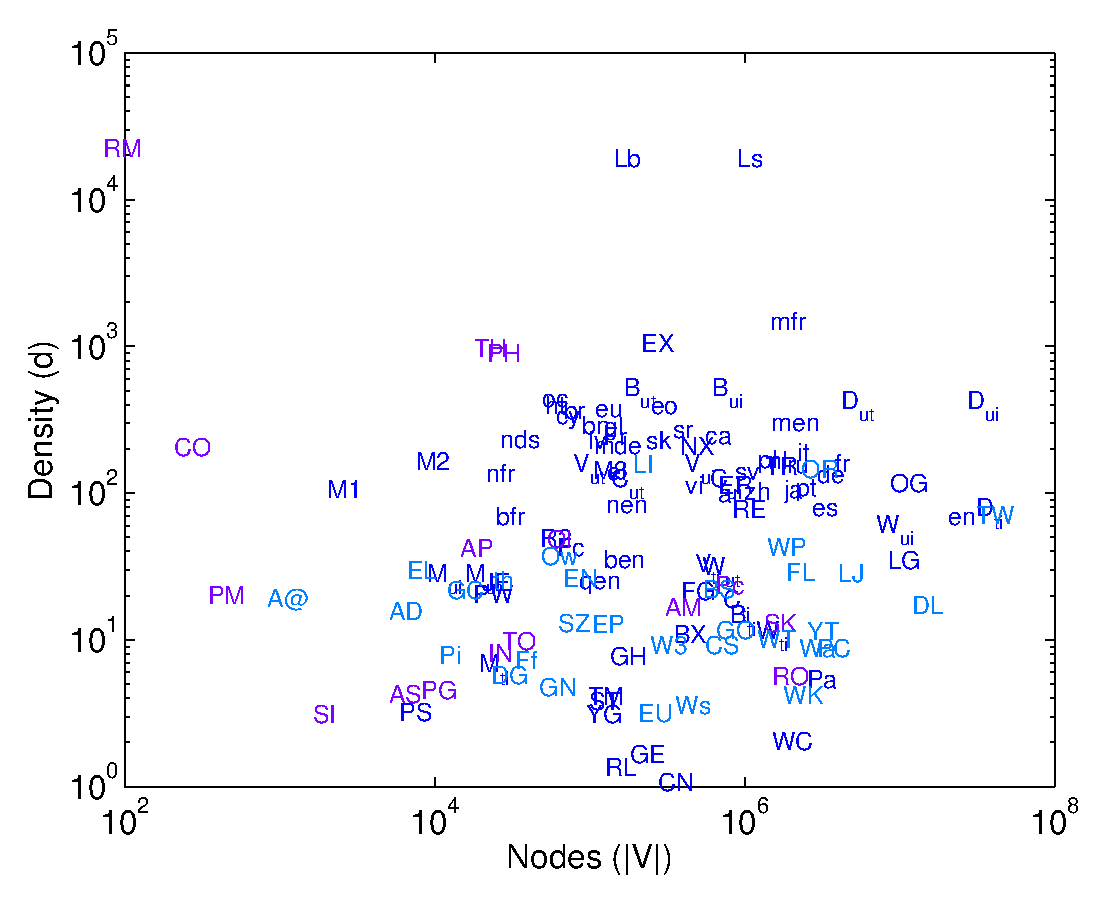
\includegraphics[width=\wTwo\textwidth] {img-st/scatter.density.a}
  }
  \subfigure[All bipartite networks by nodes]{
    \label{fig:scatter.entities}
    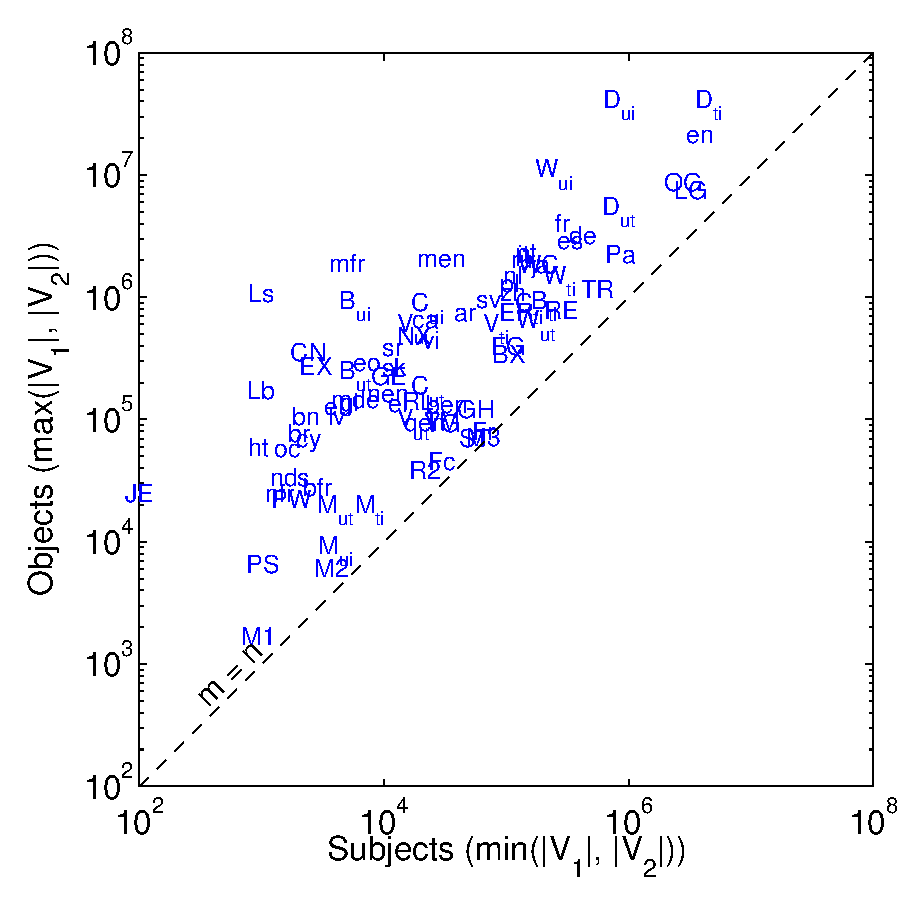
\includegraphics[width=\wTwo\textwidth] {img-st/scatter.entities.a}
  }
  \caption{
    An overview of the size of all datasets. (a)~All networks by the
    number of nodes and the density, defined as the mean number of
    neighbors for each node. (b)~All bipartite networks and bipartite
    subgraphs of folksonomies by the two node counts. 
  }
  \label{fig:scatter.relationships}
\end{figure}

Figure~\ref{fig:scatter.entities} shows all bipartite
datasets arranged by the count of both vertex types.  The most skewed
bipartite networks are Jester (\textsf{JE}) and the French Wiktionary
(\textsf{mfr}) with few items for many 
users, and last.fm (\textsf{Ls}, \textsf{Lb}), Delicious (\textsf{D}),
Twitter (\textsf{W})
and BibSonomy (\textsf{B}), with 
many items for few users.

\subsection{Network Models}
\label{sec:network-models}
In this section, we present a brief survey of common network models
applied to our network collection. 
Properties of networks can be summarized by \emph{characteristic
  numbers}, each one describing a specific aspect of the network.  In the
literature, characteristic numbers have often been used to validate
network models, i.e.\ patterns of network growth that lead to specific
values for these characteristic numbers. 
Using characteristic numbers, networks can be identified as scale-free
networks, small-world networks and evolving networks.  We review these
three models in turn. 

\subsubsection{Scale-free Networks}
\label{sec:scale-free}
\index{scale-free network}
Real-world networks are far from being random.  A random graph as
defined by Erdős and Rényi~\cite{b569} is a graph in which it is assumed
that each edge is present with a given probability independently of the
presence of other edges.  In random graphs, the number of neighbors of a
vertex follows a binomial distribution.  However, the degree
distributions of actual networks have been observed to \emph{not} follow
a binomial distribution, making the Erdős--Rényi model unsuitable for
the modeling of real networks.  Instead, many networks were observed by
Barabási and Albert to
follow power-law degree distributions~\cite{b439}.  Such networks are
called scale-free networks.  In this section, we verify whether the
networks under study can be qualified as scale-free.

The random graph and scale-free network models both arise from a network
growth process:  Random graphs can be generated by postulating that every
edge is present with 
probability $p$, and scale-free networks by assuming that the
probability of an edge being formed is proportional to the degree of
the two connected nodes, given a degree distribution. 

\begin{figure}[h!]
  \begin{tabular}{c c c c}
    \includegraphics[width=\wFourMinusTabular\textwidth]{img-st/degree.ux.epinions} &
    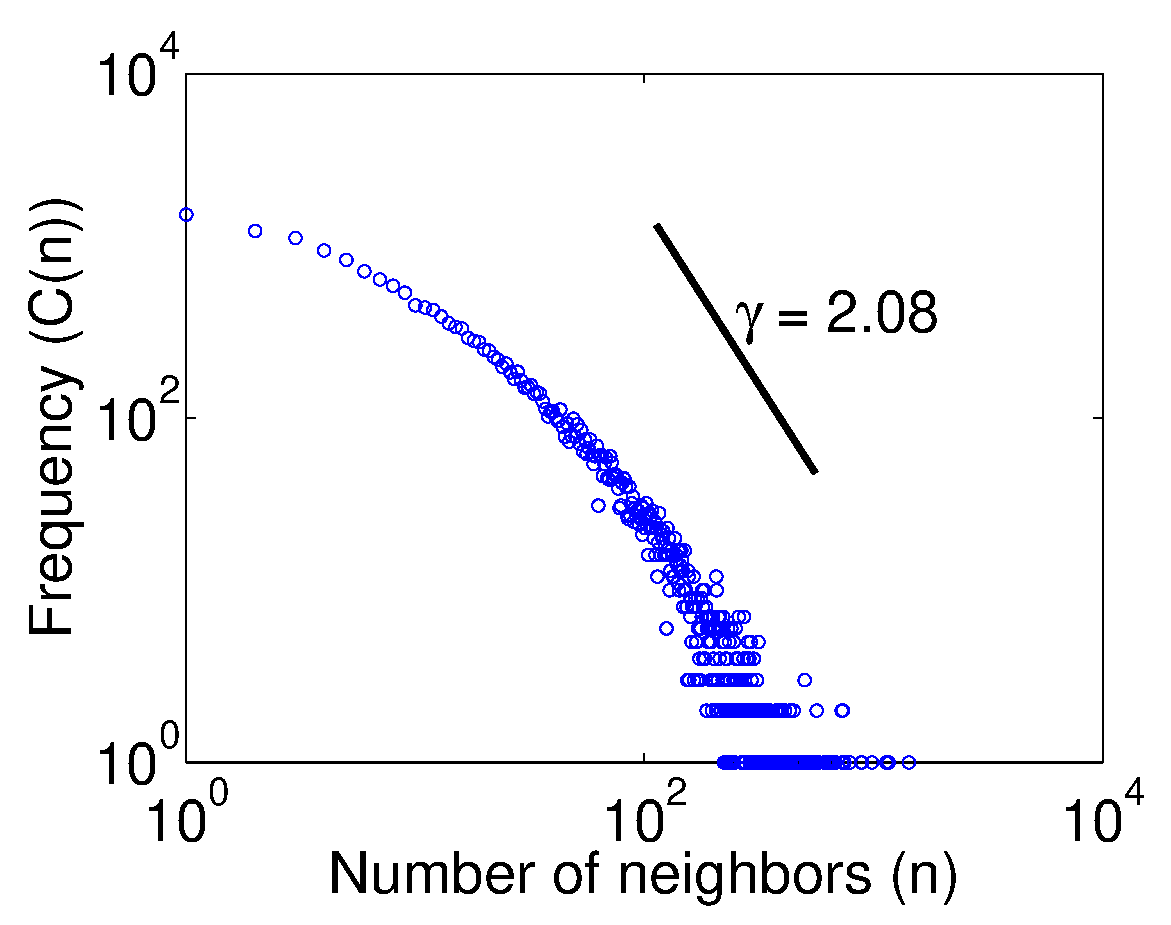
\includegraphics[width=\wFourMinusTabular\textwidth]{img-st/degree.ux.facebook-wosn-wall} &
    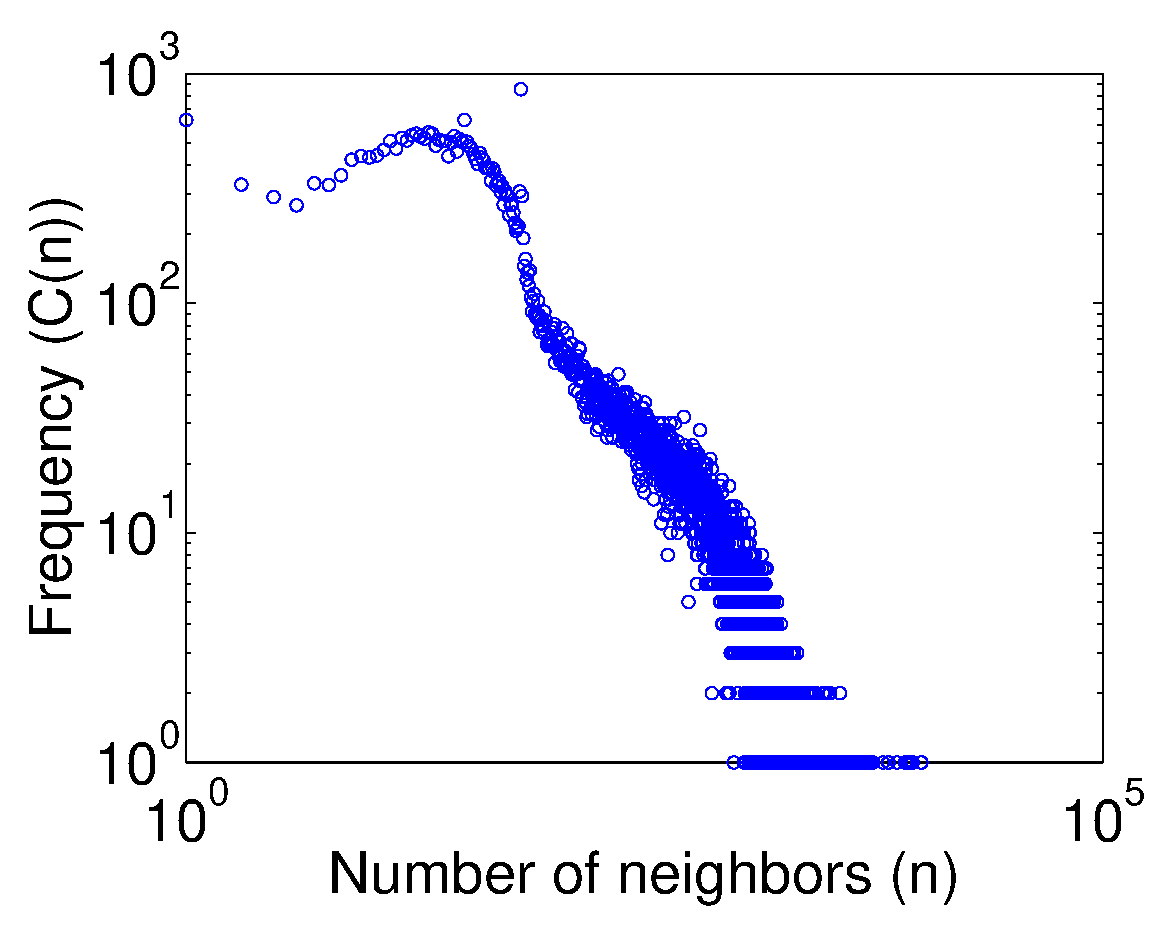
\includegraphics[width=\wFourMinusTabular\textwidth]{img-st/degree.u.filmtipset_rating} &
    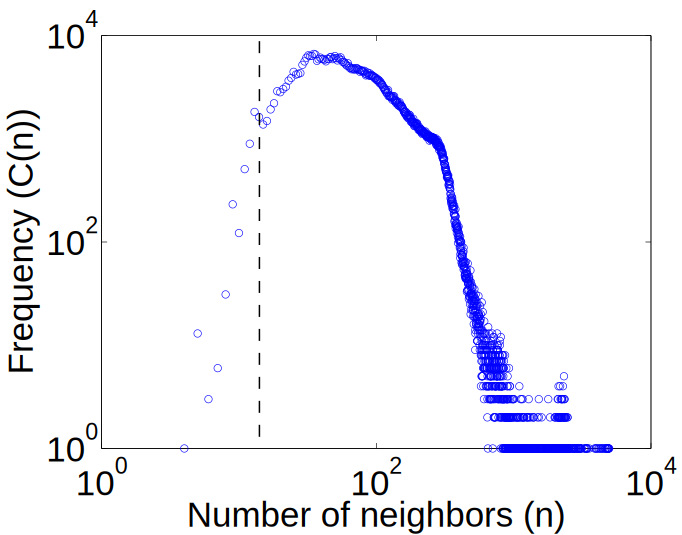
\includegraphics[width=\wFourMinusTabular\textwidth]{img-ns-svg/degree.u.reuters.limit} \\
    Epinions (\textsf{EP}) &
    Facebook (\textsf{Ow}) &
    Filmtipset (\textsf{Fr}) &
    Reuters (\textsf{RE}) \\
    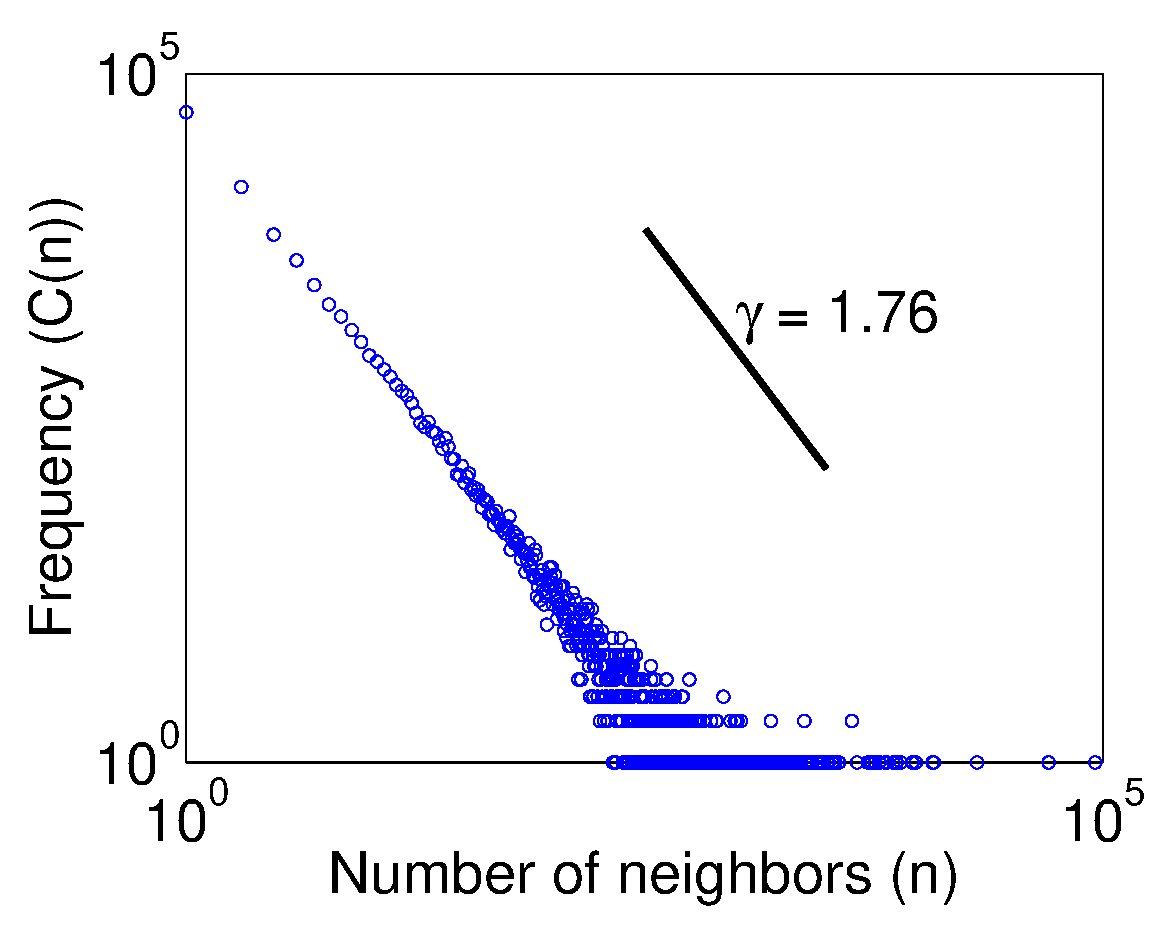
\includegraphics[width=\wFourMinusTabular\textwidth]{img-st/degree.ux.bibsonomy-2ti} &  
    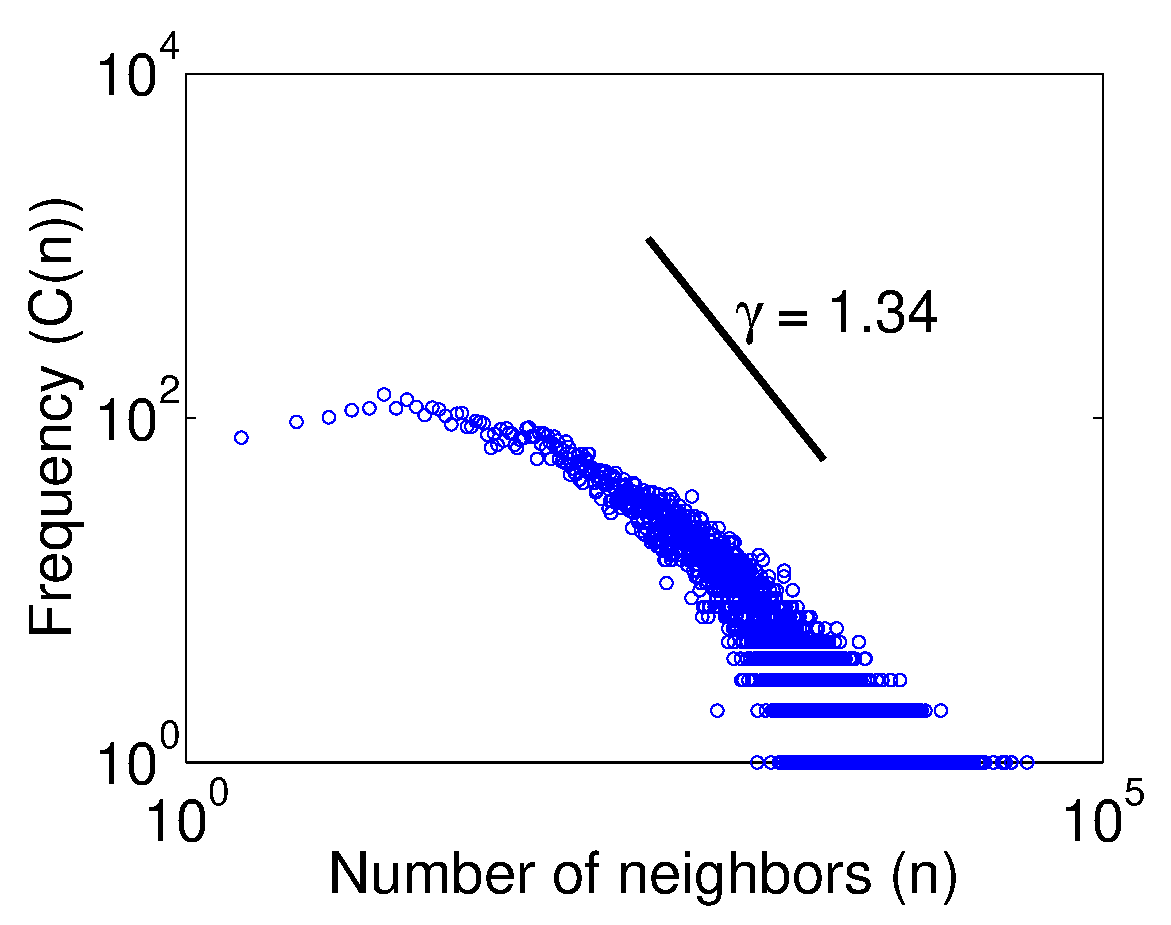
\includegraphics[width=\wFourMinusTabular\textwidth]{img-st/degree.ax.cit-HepPh} &
    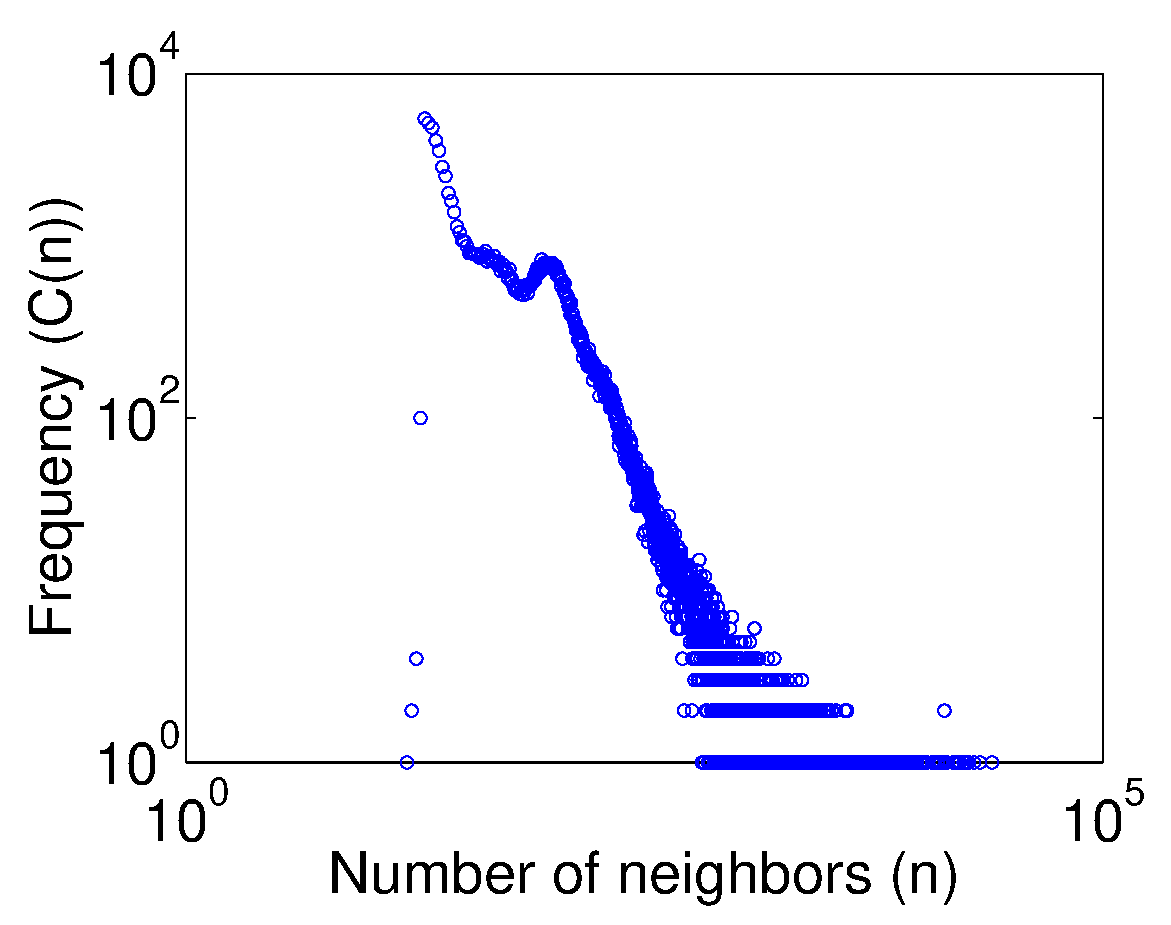
\includegraphics[width=\wFourMinusTabular\textwidth]{img-st/degree.u.libimseti} &
    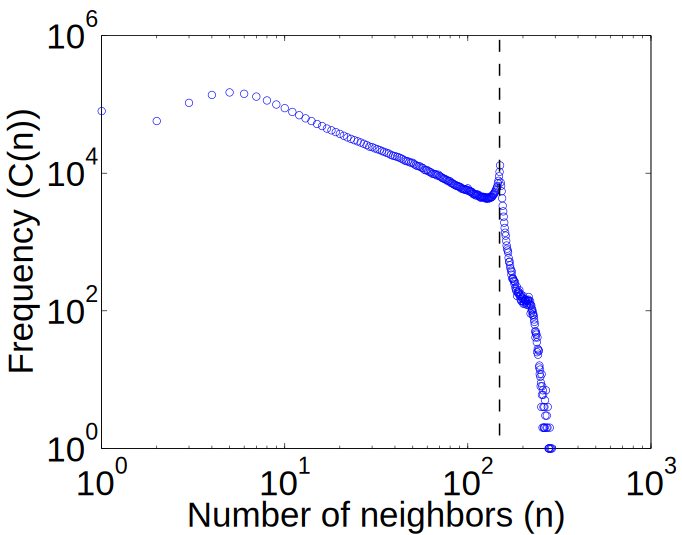
\includegraphics[width=\wFourMinusTabular\textwidth]{img-ns-svg/degree.u.livejournal-groupmemberships.limit} \\
    BibSonomy (\textsf{B$_\textsf{t}$}) &
    arXiv hep-ph (\textsf{PH}) & 
    Líbímseti.cz (\textsf{LI}) &
    LiveJournal (\textsf{LG}) \\
    \, \\
    (a) Power law &
    (b) Lognormal &
    (c) Mixtures &
    (d) Limits 
  \end{tabular}

  \caption[Diversity of degree distributions.]{
    Diversity of degree distributions observed in various networks.  
    The number of nodes $C(n)$ having exactly $n$ neighbors is
    plotted against $n$, on a double logarithmic scale. 
    The parameter $\gamma$ was estimated to fit $C(n) \sim n^{-\gamma}$
    using the method from~\cite{b408}.
    (a)~Power-law degree distributions.  
    (b)~Lognormal degree distributions.
    (c)~Mixed degree distributions.
    (d)~Degree distributions with lower and upper limits.
  }
  \label{fig:degree-distributions}
\end{figure}

Two distributions are typically studied: the distribution of vertex
degrees, and the distribution of edge multiplicities.  The degree
distribution in a scale-free network can be described by a power law,
stating that the number of nodes with $n$ neighbors is proportional to
$n^{-\gamma}$.  The constant $\gamma$ is
usually considered to characterize the preferential attachment
observed in a network, and represents an important graph characteristic.
Figure~\ref{fig:degree-distributions} shows degree
distributions for many networks, customarily drawn on a double
logarithmic scale, such that an exact power law is represented by a
line.  We observe a simple power law in many cases, but other
cases are more complex.  In certain networks, a power law is only observed for
a certain range of the distribution.  

Some degree distributions seem to
follow the discrete Gaussian exponential (DGX) model, which
corresponds to a discretized 
lognormal distribution, and is represented by an apparent squared
dependency on degree distribution plots~\cite{b319}.  In some networks,
the degree distribution seems to follow more complex patterns, which we
conjecture could be modeled as mixtures of DGX distributions.  We also
observe that \emph{passive} degree distributions are more likely to follow
power laws than \emph{active} degree distributions.  In a user--item rating
network for instance, the user degree distribution is active in the
sense that the user himself is active in giving ratings, and the item
degree distribution is passive.  We attribute this to the fact that 
active distributions are more dependent on the behavior of the
specific case.  
A unipartite example for this are citation
networks: 
In the DBLP citation dataset (\textsf{Pi}) for instance, the
distribution of the number of references peaks at 10,
whereas the number of
citations received by publications is scale-free.  
Some degree
distributions also contain artifacts of sampling, pruning methods or
limits in the number of allowed neighbors.

\begin{figure}[h!]
  \centering
  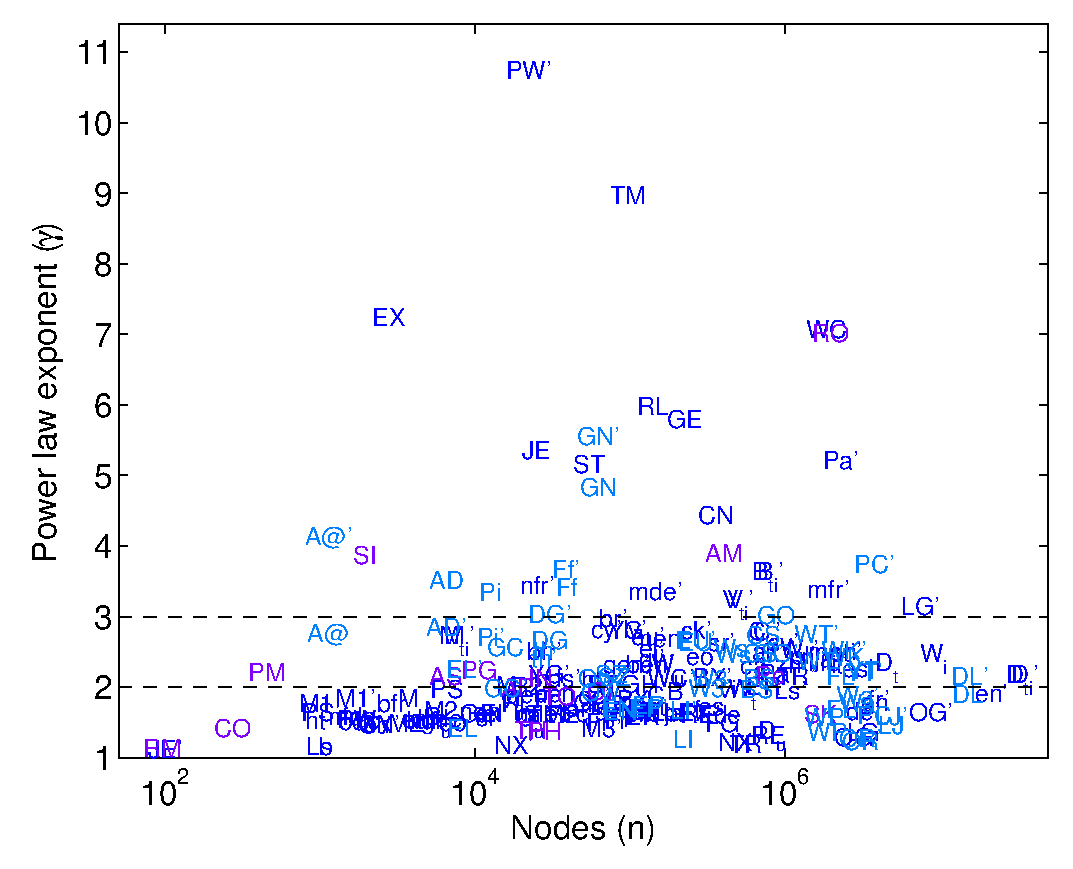
\includegraphics[width=\wTwo\textwidth]{img-st/scatter.power.a}
  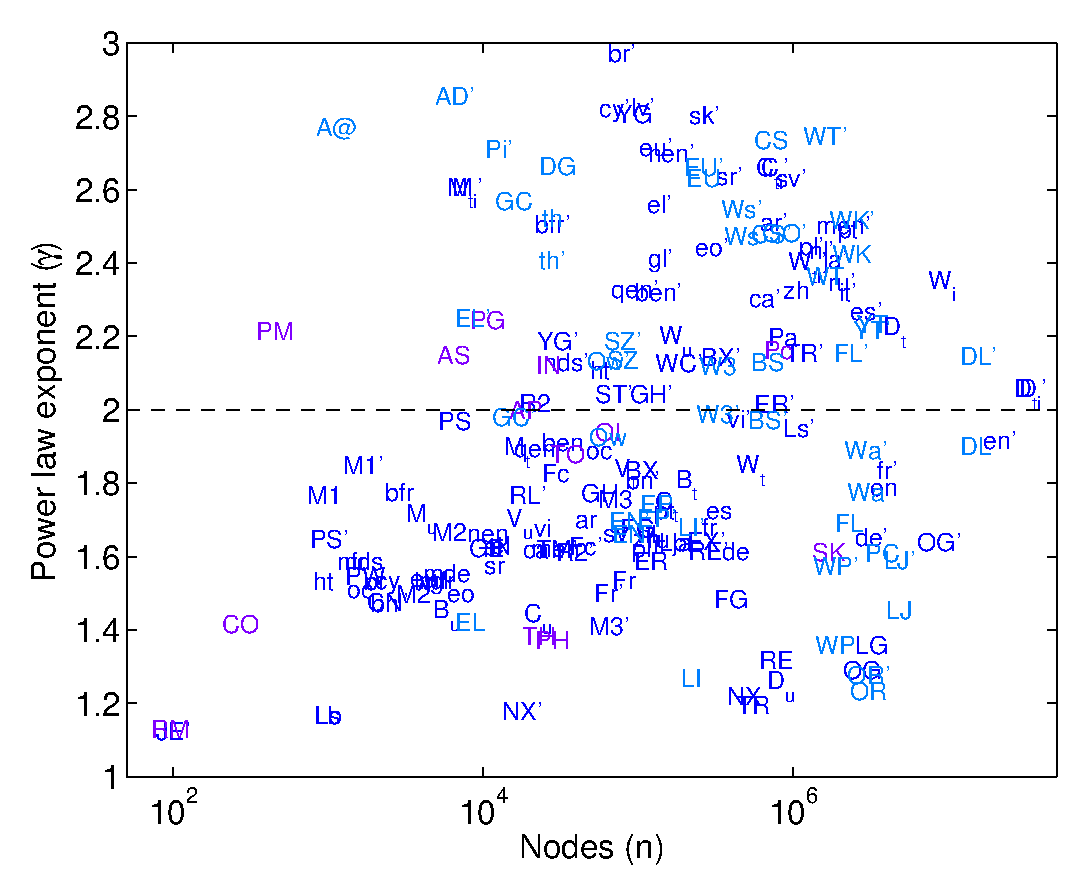
\includegraphics[width=\wTwo\textwidth]{img-st/scatter.power_detail.a}
  \caption{
    The datasets arranged by power law exponent $\gamma$.  Each
    bipartite dataset is represented twice, once for each node type.
    For object nodes in the second node set of bipartite networks, an
    apostrophe is appended to the name.  For folksonomies, the three
    exponents are marked with an index \textrm u, \textrm t or \textrm
    i.  The image on the right shows the plot restricted to $1.0 \leq
    \gamma \leq 3.0$.
  }
  \label{fig:scatter.power}
\end{figure}
If a degree distribution follows a power law, its exponent $\gamma$ can
be easily estimated~\cite{b462}.  In Figure~\ref{fig:scatter.power}, we
plot the estimated 
power law exponent $\gamma$ against the number of nodes for all unipartite
networks.  
We observe that the exponent $\gamma$ does not correlate with network
size. 
This makes the parameter $\gamma$ a scale-free network characteristic. 
Additionally, we observe that most values of $\gamma$ lie between $1.0$
and $2.0$.  This is surprising since a simple preferential attachment
model is characterized by a value of $\gamma=3.0$, and most extended
preferential attachment models predict a value in the interval~$[2.0,3.0]$. 
Most published values for $\gamma$ are also in this range, see for
instance Table~I in~\cite{b408}. 
On the other end of the scale, the listings of Prosper.com (\textsf{PW}) have numbers of
members that watch them following a power-law with exponent
$\gamma=10.7$.  In other words, only very few listing are watched by
many members and the very large majority of listings is watched by only a
few members. 

\begin{figure}[h!]
  \centering
  \begin{tabular}{c c c}
    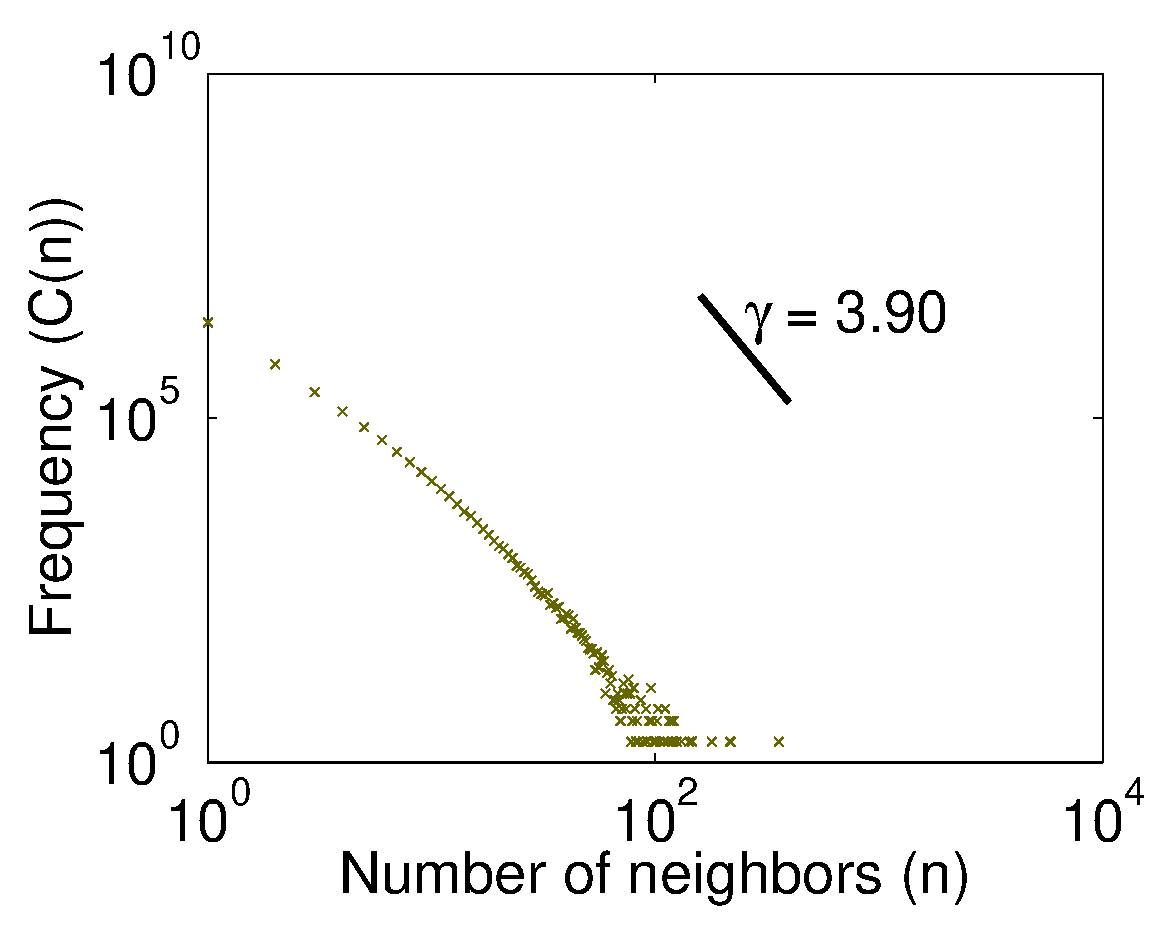
\includegraphics[width=\wThree\textwidth]{img-st/degree.weightx.dblp_coauthor} &
    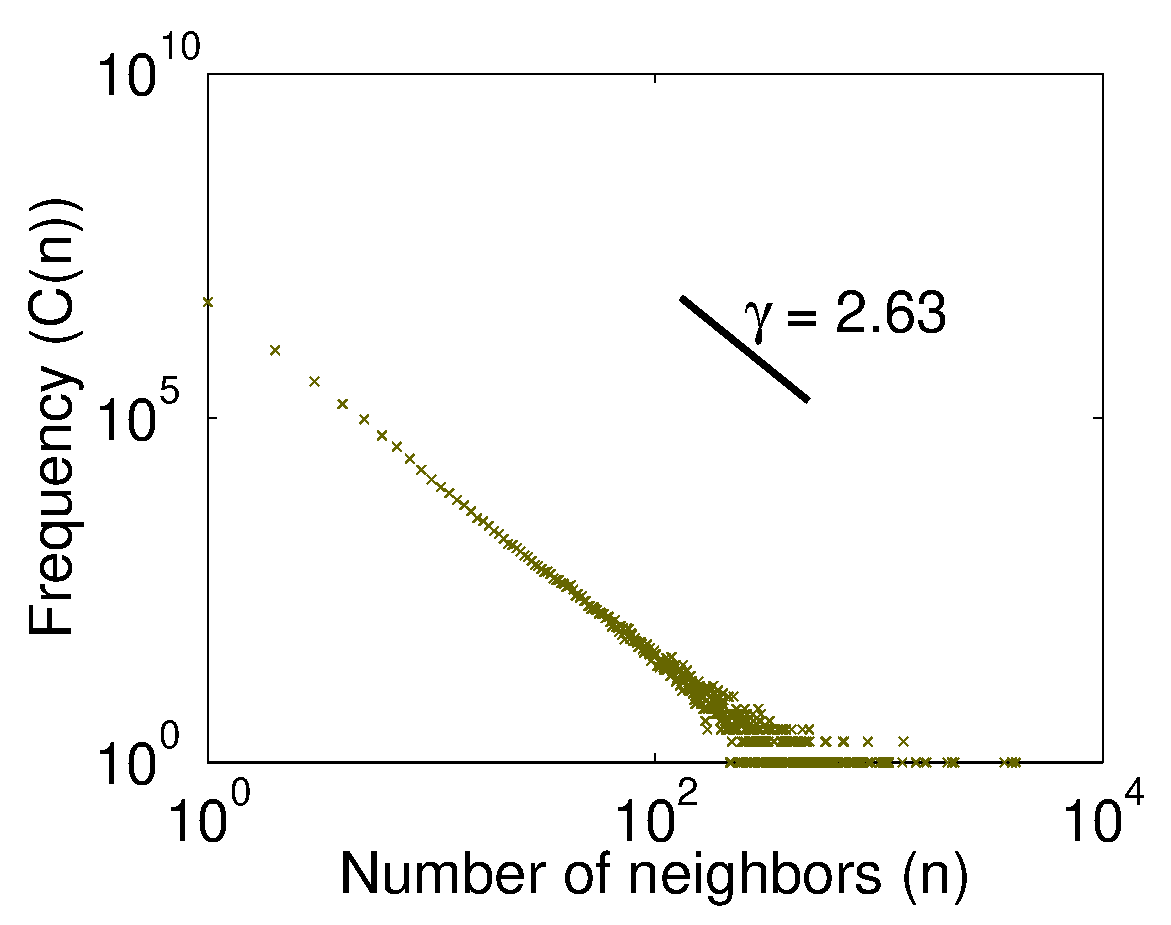
\includegraphics[width=\wThree\textwidth]{img-st/degree.weightx.edit-ptwiki} &
    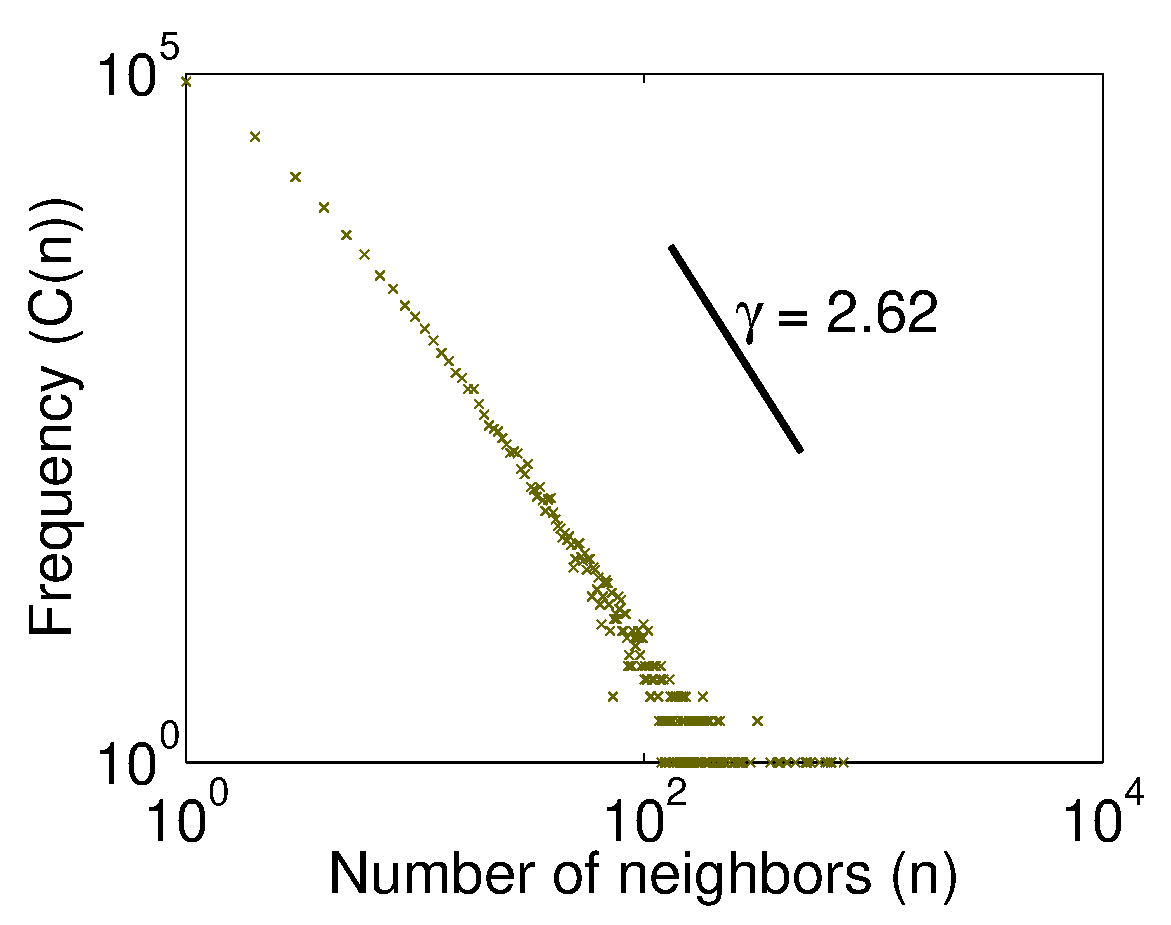
\includegraphics[width=\wThree\textwidth]{img-st/degree.weightx.facebook-wosn-wall} \\
    DBLP (\textsf{Pc}) &
    Portuguese Wikipedia (\textsf{pt}) &
    Facebook (\textsf{Ow})
  \end{tabular}
  \caption{
    Examples of edge multiplicity distributions.  
    In these plots, the number of edges having multiplicity $C(n)$ is
    plotted against $n$, on a double logarithmic scale. 
    The parameter $\gamma$ was estimated to fit $C(n) \sim n^{-\gamma}$
    using the method from~\cite{b408}.
  }
  \label{fig:multiplicity-distributions}
\end{figure}

Figure~\ref{fig:multiplicity-distributions} shows the distribution of
edge multiplicities. 
For unweighted networks with multiple edges between node pairs, we
observe edge multiplicity 
distributions to follow power laws closely, although some variations are
apparent. 
In datasets with weighted edges (of which none has multiple edges), the
distribution of edge weights is much less regular.  Although weighted
edges can be related to multiple edges by interpreting the number of
parallel edges as an edge weight, networks with natively weighted edges
apparently do not follow any consistent weight distribution. 

\subsubsection{Small-world Networks}
\label{sec:small-world}
\index{small-world network}
In the previous section, we measured the degree distribution in order to
characterize a network.  The degree distribution is however
only a \emph{local} metric, capturing single nodes and their neighborhood.
Most processes in networks are however 
\emph{global}, such as routing, link prediction, flow and diffusion.  To study
these phenomena, we must look at global properties of networks. 

Routing, flow and diffusion can be modeled as information being passed
from one node to the next along edges in the network.  To study their behavior on a
network-wide scale thus requires us to look at paths through the
network. We can thus consider two properties of paths:  Their length when they
span the whole network, and the probability of them being present.   
The typical length of paths across a network is made precise by the
\emph{network diameter}, 
which is defined as the maximum length of all shortest paths connecting
any two nodes. 
The probability of an edge appearing between
two nodes with a common neighbor is called the \emph{clustering
  coefficient}. 

In 1998, Watts and Strogatz~\cite{b228} inspected the characteristic
path length and  
clustering coefficient of several networks and made a surprising
observation:  The characteristic path length is much lower than
predicted, whereas
the clustering coefficient is much higher than predicted.  This
contradicted several previous random graph models, in particular those
where edges are randomly distributed and those that are completely
regular, forming a lattice.  By starting with a regular lattice and
randomly rewiring edges to connect random vertices, they were able to
reproduce networks with low characteristic path lengths (due to rewiring) and high
clustering coefficients (due to the initial lattice).  This model became
known as the small-world network model. 
The small-world phenomenon is most famously 
illustrated by the \emph{six degrees of separation}, made famous in
1967 by social psychologist Stanley Milgram~\cite{b567,b568}. 
Since then, six degrees of separation have been consistently reported in newer
studies for even the largest social networks~\cite{b418}.  

We can now estimate to what extent our datasets are small-world networks by
comparing their characteristic path lengths and clustering coefficients. 
Definitions of both measures vary slightly in the literature.
Here, we use the following definitions:

\paragraph{Effective Diameter}
\label{para:effective-diameter}
\index{diameter} 
\index{effective diameter}
\index{diameter}
To indicate the characteristic path length, we use the 90-percentile
effective diameter $\delta_{0.9}$, which denotes in how many steps one can reach,
on average, 90\% of all other nodes, and interpolating between adjacent
path length values.  The effective diameter can be considered a robust
extension of the actual diameter, which suffers from being skewed by
long chains~\cite{b242}.  
As an alternative, the mean shortest path
length between any two nodes is sometimes used.  

\paragraph{Clustering Coefficient} 
\index{clustering coefficient}
The clustering coefficient of a network is the probability that two
adjacent edges in that network are completed by a third edge to form a
triangle.  Let $G=(V,E)$ be an unweighted, undirected graph.  Then the
clustering coefficient is defined as:
\begin{align}
  c &= \frac
  {\left|\{ (i,j,k) \mid \{i,j\} \in E, \{j,k\} \in E, \{i,k\} \in E \}\right|}
  {\left|\{ (i,j,k) \mid \{i,j\} \in E, \{j,k\} \in E \}\right|}
\label{eq:clustering-coefficient}
\end{align}
Instead of the                  
clustering coefficient $c$, we use the relative clustering coefficient
$c_{\mathrm{rel}}$, equal to the clustering coefficient divided by
the fill of the 
network.  The fill of the network is the proportion of possible edges
that are present, and corresponds to the expected value of the
clustering coefficient when edges are distributed randomly as in the
Erdős--Rényi model. 
\begin{align}
  c_{\mathrm{rel}} &= \frac 1 {|E|/|V|^2} c
\end{align}
As a result, $c_{\mathrm{rel}}$ is larger than $1.0$
when the clustering coefficient is larger than expected in a random
graph.  
Due to the division by the fill, the relative clustering coefficients of
different networks can be compared even if the networks have different
sizes. 

The resulting scatter plot is shown
in Figure~\ref{fig:scatter.smallworldnorm}, where the more
\emph{small-world} networks are at the top-left. 
The plot shows that almost all datasets are small-world networks, but
some more than others.  This is the case for instance for the Wikipedia
talk network (\textsf{WK}). On the other hand, the Gnutella (\textsf{GN})
and Pretty Good Privacy (\textsf{PG}) networks are much less small-world
networks.  One network though is not a small-world network: the California road
network~(\textsf{RO}).  Since a road network is physically a mesh, its diameter is
very high (492), and the network is thus not a small world.  
The
second largest effective diameter is found in the DBpedia similarity
network (\textsf{SI}), and is about $16.0$. 
Then, the Berkeley/Stanford
hyperlink dataset (\textsf{BS}) has diameter around 10.5.  Generally, we find
hyperlink networks to have high diameters, in accordance with Albert et
al.~\cite{b396}, where a value of 11.2 is reported for a network of 800
million web pages.  The collaboration networks of arXiv (\textsf{PH}, \textsf{TH}) have a
small diameter, but also a small clustering coefficient.  In accordance
with the well-known \emph{six degrees of separation} observation, the
diameter of the social networks varies in the range $[5.0,7.0]$ except for
Advogato~(\textsf{AD}) and the English Wikipedia (\textsf{EL}), which have lower diameter.
We can also read from the plot that Líbímseti.cz (\textsf{LI}) and the metabolic
network (\textsf{PM}) have small-world characteristics near to a random graph,
and that the two hyperlink networks (\textsf{BS}, \textsf{WT}) are more lattice-like.

\begin{figure}[h!]
  \centering
  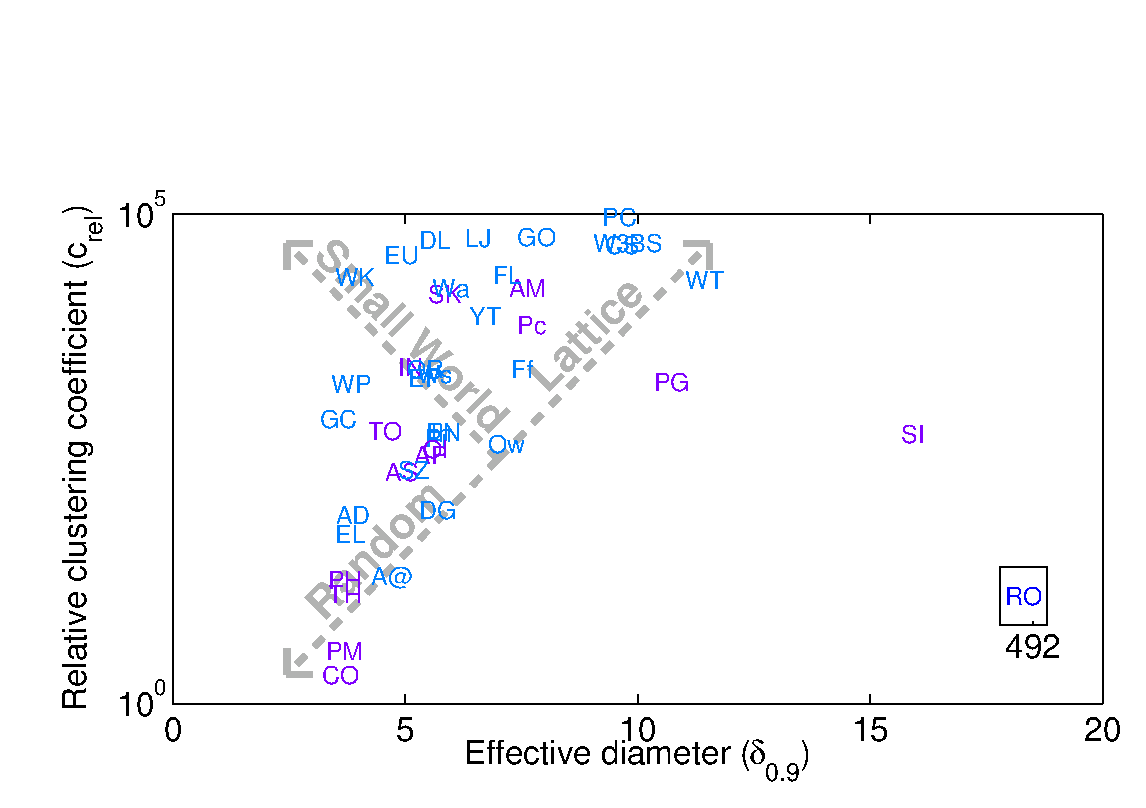
\includegraphics[width=\wOnePointFive\textwidth]{img-st/scatter.smallworldnorm.a}
  \caption{
    Verifying the small-world hypothesis:  The datasets arranged
    by diameter and relative clustering coefficient. 
    The California road network (\textsf{RO}) is outside of the main plot; its
    effective diameter $\delta_{0.9}$ is about 492.   
  }  
  \label{fig:scatter.smallworldnorm}
\end{figure}

\subsubsection{Evolving Networks}
Most networks are the result of an evolution process.  It is therefore
interesting to study the change of network characteristics over
time.  In addition to the rate of edge creation, several
non-trivial patterns have been observed in several types of networks, in
particular that 
the network density increases and the diameter decreases~\cite{b242}. 
Only for a subset of all datasets the edge creation times are known; 
Table~\ref{tab:datasets} gives the complete list. 

Network dynamics is an important aspect in network analysis because it directly
leads to link prediction algorithms in the following way:  If a certain
pattern is observed in the temporal dynamic of the networks,
extrapolating this pattern into the future directly gives a prediction
for the future appearance of edges.  Being able to predict links in a
network then allows one to implement virtually all types of recommender
systems. 

\begin{figure}[h!]
  \centering
  \begin{tabular}{cc}
    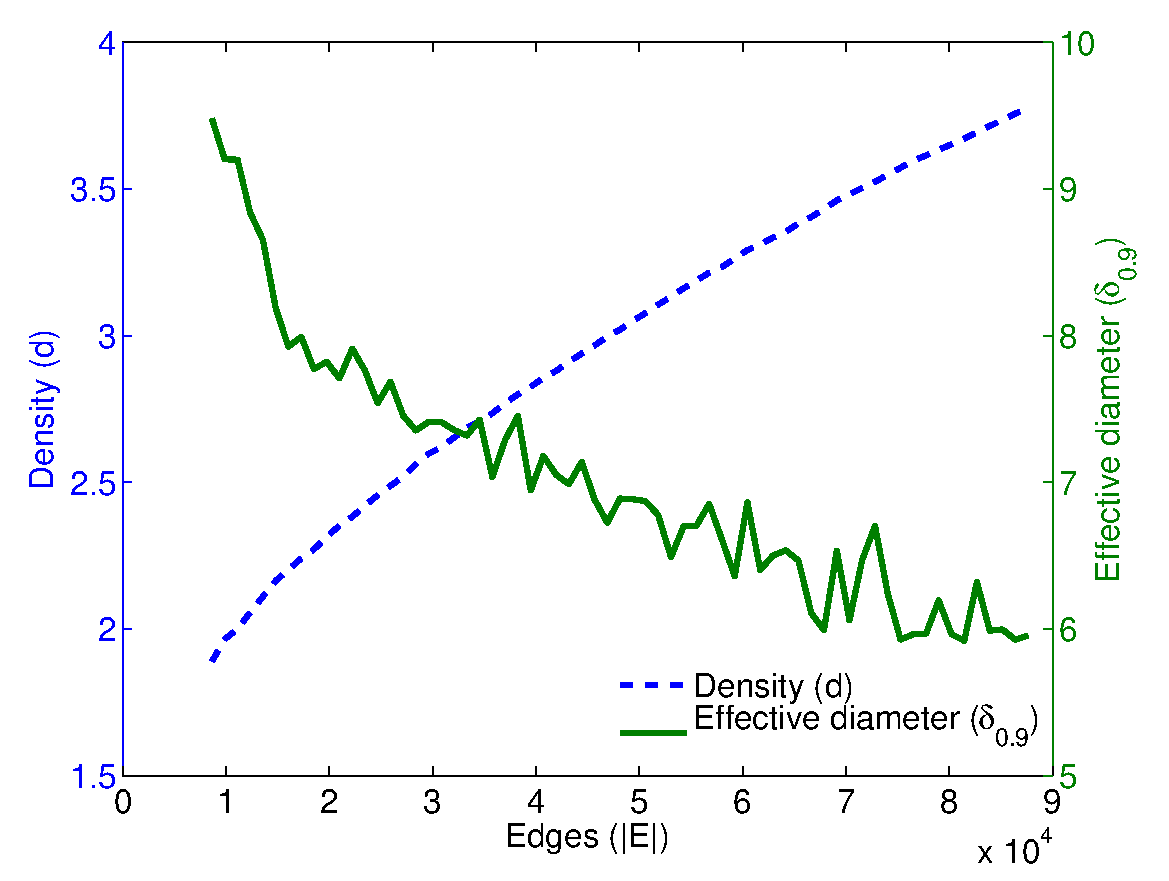
\includegraphics[width=\wTwo\textwidth]{img-st/diadens.munmun_digg_reply} &
    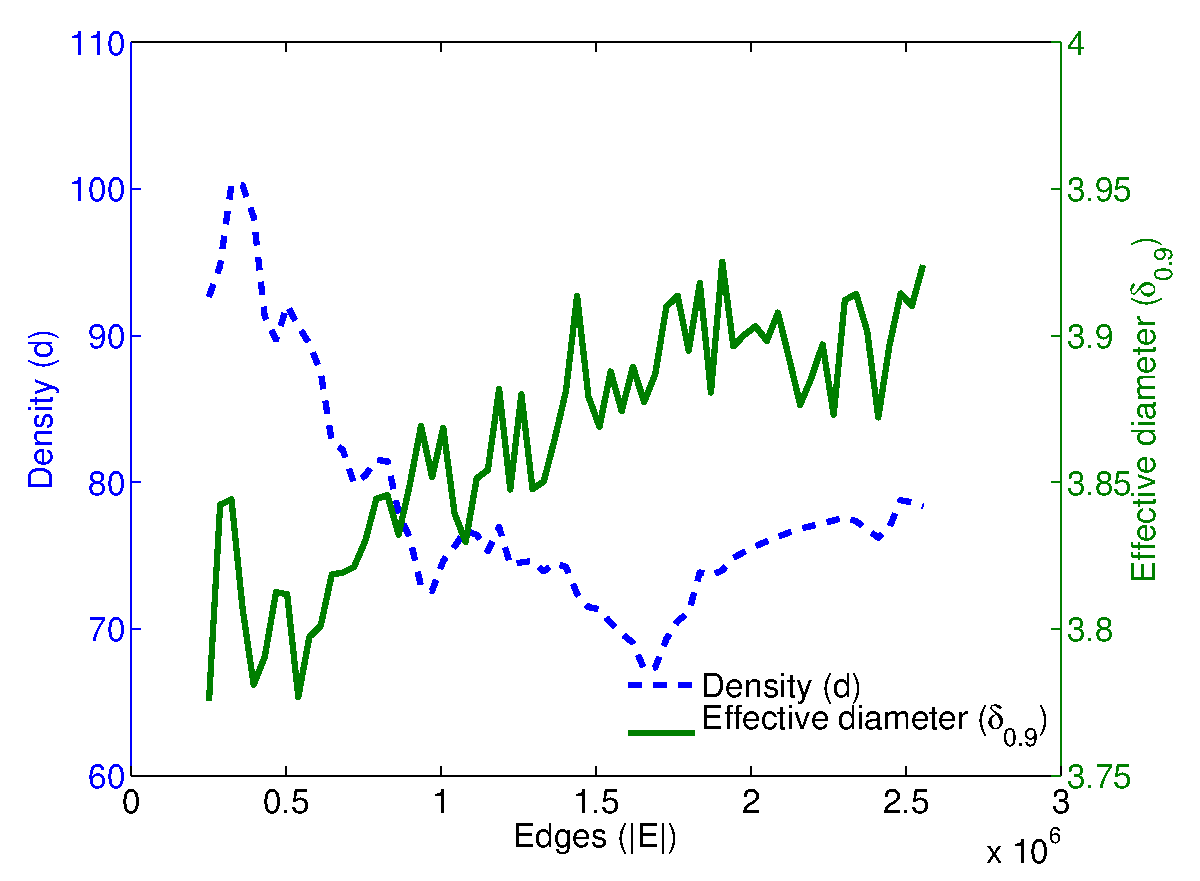
\includegraphics[width=\wTwo\textwidth]{img-st/diadens.bibsonomy-2ut} \\
    Digg (\textsf{DG}) &
    BibSonomy (\textsf{B$_{\mathrm{ut}}$})
  \end{tabular}

  \caption{
    Evolution of network characteristics over time.  For two networks,
    we show, in function of the number of edges $|E|$ in the network, the
    network's density $d$ and the effective diameter $\delta_{0.9}$. 
  }
  \label{fig:evolution}
\end{figure}

In~\cite{b242}, Leskovec et al. studied the evolution of network
characteristics over time and made the following observations: The
diameter of graphs seems to \emph{shrink} and the density to
\emph{grow}.  This result is surprising, since a scale-free model would
indicate at least the diameter to increase with network size.  We verify
this behavior for our datasets in Figures~\ref{fig:evolution}
and~\ref{fig:scatter.diadens}.  The behavior of the density and the
diameter in our datasets is generally as predicted in~\cite{b242}, where
it is derived from a graph growth model called \emph{forest fire}.  We
observe the Netflix (\textsf{NX}), Digg (\textsf{DG}), YouTube
(\textsf{YT}), Internet topology (\textsf{TO}), Facebook (\textsf{OI})
and Last.fm (\textsf{Ls}, \textsf{Lb}) networks to clearly show
shrinking diameters in conjunction with increasing density.  On the
other hand, Enron (\textsf{EN}) and BibSonomy (\textsf{B}) display the
opposite behavior.  We therefore observe that the forest fire model is
less universal than the scale-free and small-world models.  We also note
that there is no discernible correlation between the temporal evolution
of the diameter and density.  On another level, we confirm that
shrinking diameters and increasing density are also observed for
bipartite networks.

\begin{figure}[h!]
  \centering
  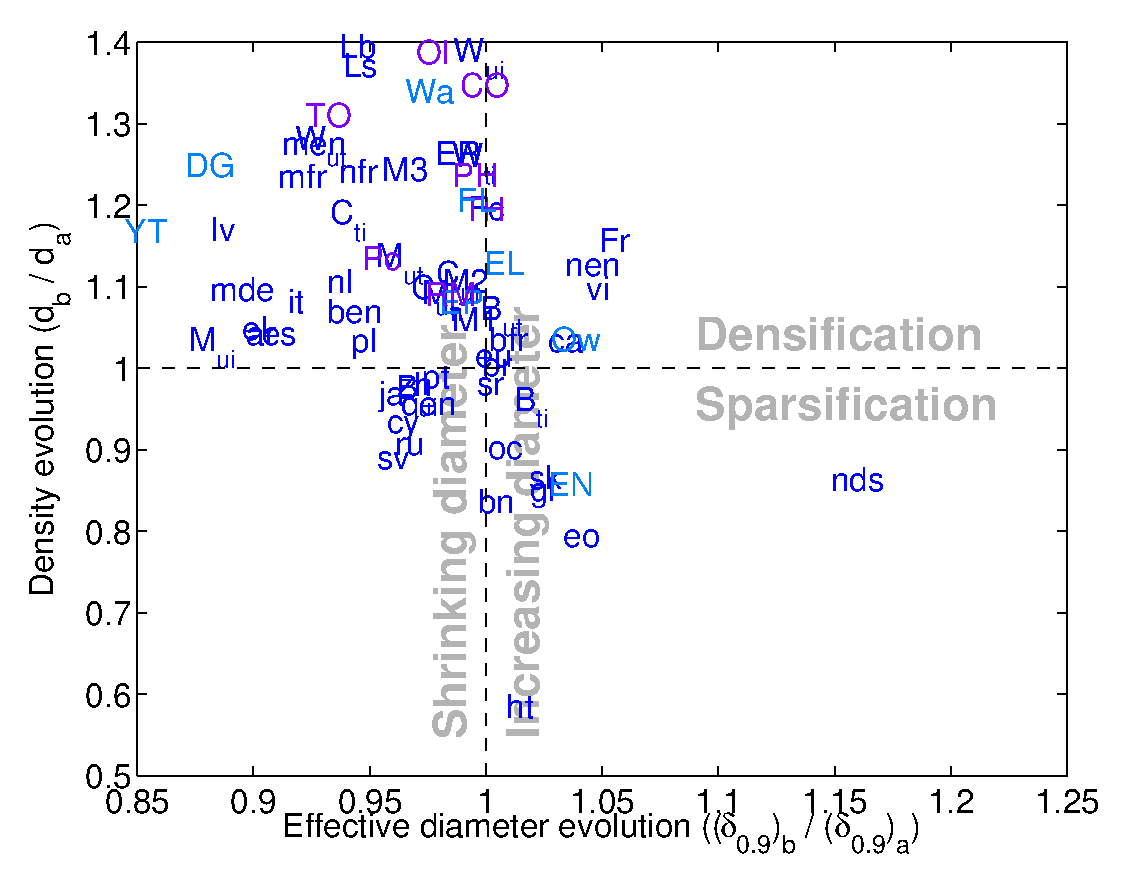
\includegraphics[width=\wTwo\textwidth]{img-st/scatter.diadens.a}
  \caption{
    The evolution of the diameter $\delta_{0.9}$ and density $d$ over time.
    This plot compares the ratio of the diameter and
    density of the complete networks ($(\delta_{0.9})_{\mathrm b}$ and
    $d_{\mathrm b}$) and of the network 
    containing half of all edges ($(\delta_{0.9})_{\mathrm a}$ and $d_{\mathrm
      a}$).  Only networks with 
    timestamps are shown.  
  }
  \label{fig:scatter.diadens}
\end{figure}

\subsection{The Slashdot Zoo}
\label{sec:zoo}
\index{Slashdot Zoo}
\index{friend and foe}

In addition to the numerous publically available network datasets listed
in Appendix~\ref{chap:datasets}, one network dataset was extracted
during the course of writing this thesis: the Slashdot Zoo~(\textsf{SZ}).
Slashdot\footnote{\href{http://slashdot.org/}{slashdot.org}} is a
technology news website founded in 1997.  It publishes stories written
by editors or submitted by users and allows users to comment on them.
In 2002, the site added the \emph{Zoo} feature, which lets users tag
other users as \emph{friends} and \emph{foes}.  In contrast to most
popular social networking services, Slashdot is one of the few sites
that also allows users to rate other users negatively.  
The Slashdot Zoo dataset is available
online\footnote{\href{http://dai-labor.de/IRML/datasets}{dai-labor.de/IRML/datasets}}.


The Slashdot Zoo network we extracted contains 77,985 users and 510,157
links.  Each link consists of a user who gave an endorsement and a user
who received the endorsement.  Endorsements can be either positive
(\emph{friend}) or negative (\emph{foe}).  Apart from this distinction, no
other information is available; in particular, the creation date of
endorsements is not known.
In addition to the terms \emph{friend} and \emph{foe}, Slashdot also uses the
terms \emph{fan} and \emph{freak}:  A user is always the fan of his friends
and the freak of his foes.  Figure~\ref{fig:ffff} summarizes these
relationships. 

\begin{figure}[h!]
  \centering
  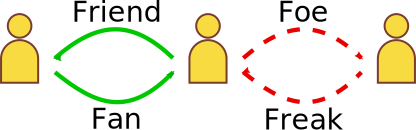
\includegraphics[width=\wTwo\textwidth]{img-svg/friends-foes}
  \caption{
    The two types of links allowed in the Slashdot Zoo (friend and foe)
    give rise to four kinds of relationships: friends, fans, foes and
    freaks.  A user is the fan of his friends and the freak of his foes.
  }
  \label{fig:ffff}
\end{figure}

Figure~\ref{fig:layout} is a graphical representation of the Slashdot
Zoo network.  The sign of an edge is represented by its color, with green
representing the \emph{friend} relationship and red representing the
\emph{foe} relationship.  The graph is centered at user \emph{CmdrTaco}, founder
of Slashdot and active editor. 
While most social network modeling approaches allow for weighted edges,
the weights are usually restricted to positive values.  However, some
relationships such as distrust and dislike are inherently negative.  In
such cases, the social network contains \emph{negative edge weights}.
This is the case for the Slashdot Zoo, and will be described in
Chapter~\ref{chap:signed}. 

\begin{SCfigure}
  \centering
  \includegraphics[width=\wTwo\textwidth]{img-eps/out2_gross__PERFECT_klein}
  \caption{
    The Slashdot Zoo network represented as a graph, where nodes
    represent users and edges indicate relationships.  The network
    contains 79,120 nodes and 515,581 edges.  \emph{friend} relationships
    are shown in green edges and \emph{foe} relationships in red; the
    orientation of edges is not shown.  The graph is centered at user
    \emph{CmdrTaco}. 
  }
  \label{fig:layout}
\end{SCfigure}

The dataset was crawled from \href{http://slashdot.org/}{slashdot.org}
between May and October 2008, and the dataset 
does not represent a true snapshot of the network, and may exhibit
anomalies.  For instance, 
because the Slashdot website does not indicate when a friend or foe was
added, 
some users in our dataset may have more than 400
friends or foes, although Slashdot generally limits the number of
friends and foes to 200 users and to 400 users for subscribers.

\index{troll}
Slashdot is known for both having very popular and prominent users on
the one hand, and rather unpopular users on the other hand.
Prominent and popular users of Slashdot include CmdrTaco (Rob Malda,
the founder of Slashdot and a popular editor), John Carmack (prominent
computer game programmer), Bruce Perens (prominent computer programmer
and open source advocate) and CleverNickName (Wil Wheaton, Star Trek
actor).  
In addition, Slashdot is well known for having a tradition of
\emph{trolling}, i.e.\ the posting of disruptive, false or offensive
information to fool 
and provoke readers.  
The high number of such trolls may explain why the \emph{foe} feature is
useful on Slashdot.  It allows for tagging known trolls and reducing
their visibility.   

\begin{figure}[h!]
  \centering
  \subfigure[Outdegree (friend and foes)]{
    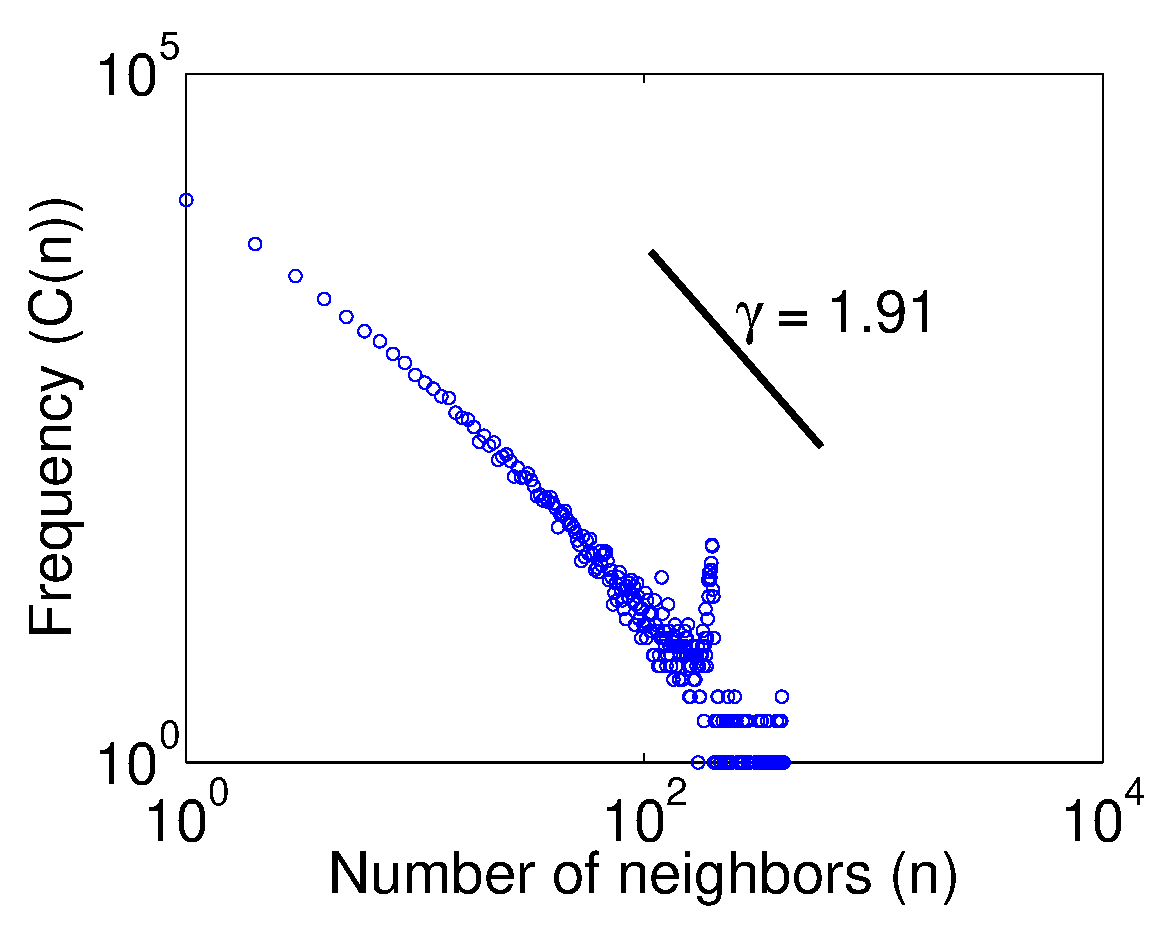
\includegraphics[width=\wTwo\textwidth]{img-st/degree.ux.slashdot-zoo}
  }
  \subfigure[Indegree (fans and freaks)]{
    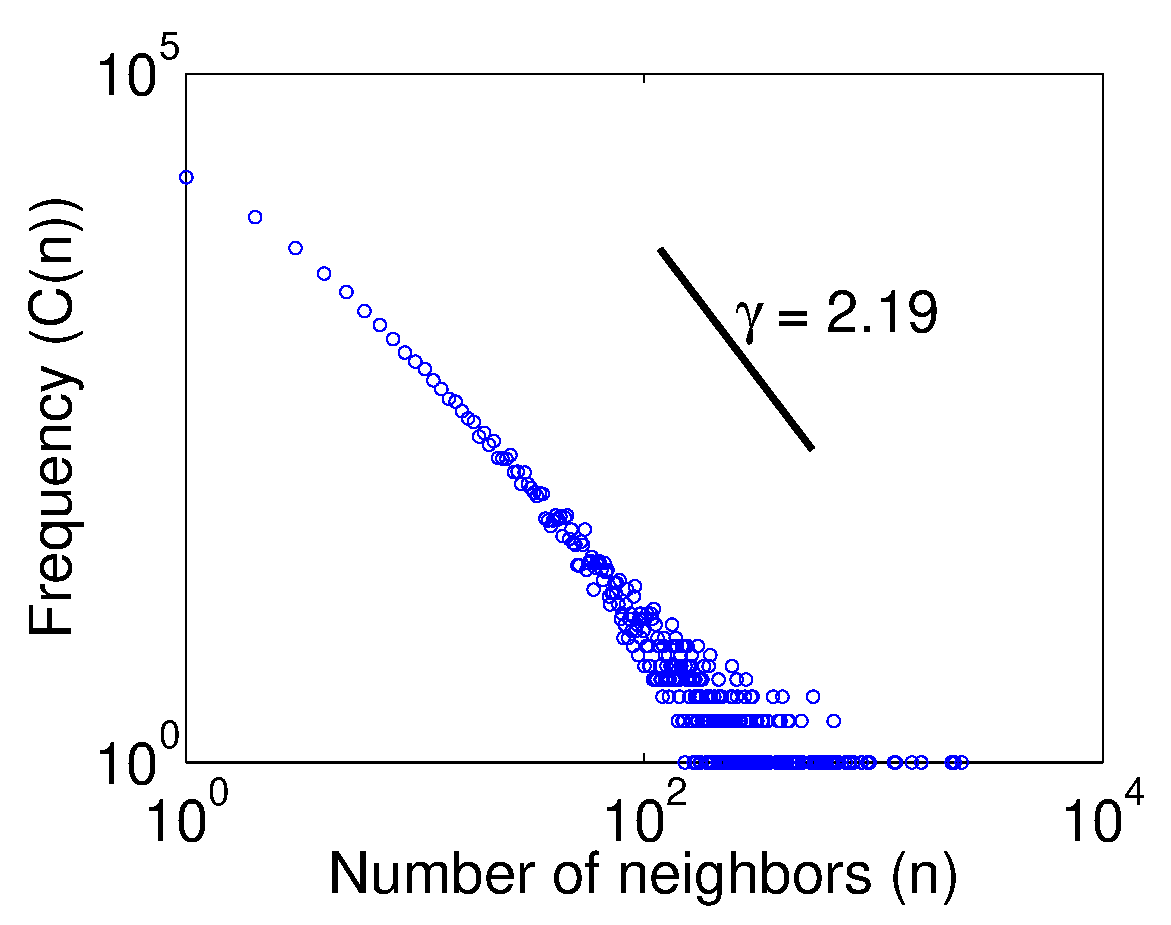
\includegraphics[width=\wTwo\textwidth]{img-st/degree.vx.slashdot-zoo}
  }
  \caption{
    Double logarithmic plot of the degree distributions in the Slashdot
    Zoo, showing that they follow a power law.  The limit of 200 friends
    and foes is visible for the outdegree plot~(a).
  }
  \label{fig:zoo-deg}
\end{figure}

Table~\ref{tab:zoo-stat} displays basic statistics of the dataset.
All distances were calculated without taking into account
the edge directions and signs.  
%% In parentheses, we show the average
%% distance.  
The measured average distance
is less than the average distance in a random graph, confirming that the
Slashdot Zoo is a small-world network.
Figure~\ref{fig:zoo-deg} shows the degree distributions in the Slashdot
Zoo.  As expected, the degree distribution in the Slashdot Zoo follows a
power law. 

\begin{table}
  \centering
  \caption{
    Statistics about the Slashdot Zoo.  The mean
    friend count and mean fan count are necessarily equal, as do the mean
    foe and freak counts.
    The sign and direction of edges was ignored
    in the calculation of the diameter and radius.
    In parentheses, we show the average distance in a random graph, as
    defined by Watts and Strogatz~\cite{b228}.
  }
  \label{tab:zoo-stat}
  \begin{tabular}{ l r }
    \toprule
    \textbf{Users} & 79,120 \\
    \midrule
    \textbf{Links} & 515,581 \\
    \textbf{Friend links} & 392,326 \\
    \textbf{Foe links} & 123,255 \\
    \midrule
    \textbf{Fill} & 0.000083884 \\
    \midrule
    \textbf{Diameter} & 6 \\
    \textbf{Radius}  & 3 \\
    \bottomrule
  \end{tabular}
  \qquad
  \begin{tabular}{lr}
    \toprule
    \textbf{Mean link count} & 6.542 \\
    \textbf{Mean friend/fan count} & 4.978 \\
    \textbf{Mean foe/freak count} &  1.564 \\
    \midrule
    \textbf{Median links} & 3 \\
    \textbf{Median friend count} & 1 \\
    \textbf{Median foe count} & 0 \\
    \textbf{Median fans count} & 1 \\
    \textbf{Median freaks count} & 1 \\
    \bottomrule
  \end{tabular}
\end{table}

\section{Summary}
Data from many diverse application areas can be modeled as networks. 
Whether they are
unipartite, bipartite, weighted, signed, directed or undirected, graphs
play a fundamental role in many disciplines because 
they can model many real-world interactions.  
We use as a testing ground in this thesis 
a collection of \input{number}network datasets. One of
these networks, the Slashdot Zoo, was specifically extracted for 
this thesis.  The Slashdot Zoo is 
a social network with positive and negative links, and will be the
basis for the analysis of 
signed networks in Chapter~\ref{chap:signed}.

\chapter{The Spectral Evolution Model}
\label{chap:spectral-evolution-model}
This chapter describes the \emph{spectral evolution model}, which
constitutes the main statement in this thesis.  The spectral evolution
model characterizes the change of a network in terms of the eigenvalue
decomposition of its adjacency matrix.  It states that over time,
eigenvalues change, while eigenvectors stay constant.  
The spectral evolution model 
is stated and verified empirically in this chapter for unweighted
undirected unipartite networks.  
The spectral evolution model serves as the basis for the two new link
prediction algorithms described in the next chapter.  
The case of 
weighted networks is described in Chapter~\ref{chap:signed} and that of
bipartite and directed networks in Chapter~\ref{chap:asymmetry}.  In the
examples of this chapter, we will also use directed networks,
but always ignore edge orientations for them.  

We begin this chapter in
Section~\ref{sec:spectral-evolution-model:definition} by deriving the
spectral evolution model from a simple link prediction model, the matrix
exponential kernel.  Then, in
Section~\ref{sec:spectral-evolution-model:verification}, we verify
the spectral evolution model empirically using our collection of network
datasets. 
After establishing that the spectral evolution model can be
observed in many networks, we show that it can be derived from
multiple models of graph growth in
Section~\ref{sec:spectral-evolution-model:explanations}, in particular
from many known graph kernels and from a generalization of the
preferential model attachment.  
These models will give intuitive and mathematical explanations for the
spectral evolution model. 
In Section~\ref{sec:spectral-evolution-model:control}, we
finally present two control tests to make sure that the spectral 
evolution model is specifically not implied by random graph models,
making the spectral evolution model a non-trivial property of real
networks.

\section{Overview}
\label{sec:spectral-evolution-model:definition}
\index{spectral evolution}
Many machine learning problems on networks can be described as link
prediction: finding movies a user might like, recommending friends, or
finding related topics in a collaboration graph.  In all these cases, a
given network is assumed to \emph{grow} over time and the task is to
predict where new edges will appear and, in some cases, to also predict
their weight.  On the other hand, any given link prediction algorithm
can be interpreted as a model of graph growth by assuming that networks
actually grow as the algorithm predicts.  In this work, we are concerned
with those link prediction algorithms that have an algebraic
description.  We show that they imply a network growth model that we
call \emph{spectral evolution}.  Our hypothesis states that in terms of
the eigenvalue decomposition of a network's adjacency matrix $\mathbf
A=\mathbf U\mathbf \Lambda\mathbf U^{\mathrm T}$, growth can be
described as a transformation of the spectrum $\mathbf \Lambda$, without
significant change in the eigenvectors~$\mathbf U$.

Each algebraic link prediction algorithm, including most graph
kernels, represents a specific assumption about network growth,
leading to a different spectral transformation function.  
Each of these link prediction functions can be applied in different
situations, depending on the assumptions made about the
network. Despite this, all algebraic link prediction algorithms are
of the same form: a change of the eigenvalues following a specific
function, without change in the eigenvectors.  Therefore, they are all
generalized by the spectral evolution model.  
Starting with a
network's adjacency matrix $\mathbf A$, we first compute its eigenvalue
decomposition 
$\mathbf A=\mathbf U\mathbf\Lambda \mathbf U^{\mathrm T}$.  It can then be shown
that many common link prediction 
algorithms can be expressed as $\mathbf U F(\mathbf\Lambda)\mathbf U^{\mathrm T}$,
where $F$ is a function 
that applies a real function $f(\lambda)$ to each diagonal
element of $\mathbf\Lambda$.

Consider the following example:
The matrix exponential of the adjacency matrix $\mathbf A$ is sometimes
used as a link prediction function~\cite{b156}.  The matrix exponential is
defined as $\exp(\mathbf A)=\sum_{k=0}^\infty \mathbf A^k/k!$, and can
be interpreted in the following way:  $\exp(\mathbf A)_{ij}$ equals a
weighted sum over all paths from the node $i$ to the node $j$ in the
network, where paths 
are weighted by the inverse of the factorial of their length. 
This description shows why the exponential of the adjacency matrix is a
suitable link prediction function:
\begin{itemize}
\item The link prediction score is higher when there are many paths
  between $i$ and $j$, because the powers of $\mathbf A$ count the
  number of paths.
\item The link prediction score is higher when these paths are short,
  because the weights $1/k!$ are decreasing. 
\end{itemize}
The matrix exponential can also be written in terms of the eigenvalue
decomposition $\mathbf A = \mathbf U \mathbf \Lambda \mathbf U^{\mathrm
  T}$ as
\begin{align*}
  \exp(\mathbf U\mathbf \Lambda \mathbf U^{\mathrm T}) &= \mathbf U \exp(\mathbf
  \Lambda) \mathbf U^{\mathrm T},
\end{align*}
where $\exp(\mathbf \Lambda)$ can be computed by applying the real exponential
function to $\mathbf \Lambda$'s diagonal elements.  
This shows that the matrix exponential is a spectral transformation of
the adjacency matrix $\mathbf A$.
We will see later that several other link prediction functions can be
expressed as spectral transformations in an analogous way.  First however, we state the
spectral evolution model.

\begin{mydef}[Spectral evolution model]
  A network that changes over time is said to follow the spectral
  evolution model when its spectrum evolves while its eigenvectors stay
  approximately constant. 
\end{mydef}

This definition is not mathematically strict.  Whether a network
conforms to the spectral evolution model depends on the interpretation
of when an eigenvectors stays \emph{approximately constant}.  This
fuzziness will be made 
precise in Section~\ref{sec:spectral-evolution-model:control}.  For now,
we will interpret the 
definition loosely, taking eigenvectors as approximately constant when
their change is small. 
The spectral evolution model is visualized schematically in
Figure~\ref{fig:sne-overview}:  In this simplified picture, a small network
to which edges are added consecutively has three different spectra at
three different times, but the same set of eigenvectors at all times. 

\begin{figure}[h!]
  \centering
  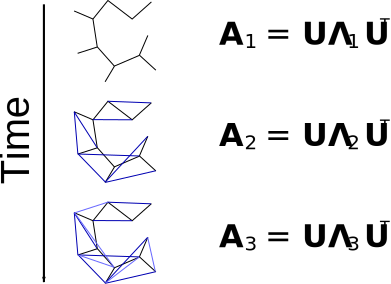
\includegraphics[width=\wTwo\textwidth]{img-svg/sne-overview}
  \caption{
    Illustration of the spectral evolution model. 
    As edges appear in a network, the eigenvalues of the network's
    adjacency matrix change, while the eigenvectors stay constant. 
  }
  \label{fig:sne-overview}
\end{figure}

To examine the validity of the spectral evolution model, we 
take three steps.  First, we verify it empirically in our collection
of datasets.  Then, we review existing link prediction functions that
imply the spectral evolution model and finally, we present control tests
to verify that the spectral evolution model does not arise from other
processes, such as random graph growth. 

\section{Empirical Verification}
\label{sec:spectral-evolution-model:verification}
Which network model does accurately describe the growth of real networks?  Given
a network, which link prediction function does best model its growth?  To answer these
questions, we examine the spectra of large, real-world networks and
observe their temporal evolution.
In the following sections, we look at the evolution of the
eigenvalue decomposition of the networks given in
Table~\ref{tab:datasets} in Appendix~\ref{chap:datasets}. 

For each network, we split the set of edges into $\totaltime=75$ bins by
edge creation 
time.  For each bin, we take the network as it was after the arrival of
that bin's edges, and compute the first $\syRank$ eigenvalues of
the resulting adjacency matrix. 
In the networks we study in this chapter, 
the creation times of edges are known.  
%% The set of edges is split into 
%% timeslices, and at 
%% each timeslice, the $\syRank$ dominant eigenvalues are computed.  
$\syRank$ is
chosen in function of network size to give reasonable runtimes.
We denote by $\mathbf A_{t}$ the adjacency matrix of all edges present
after time~$t$.  Thus $\mathbf A_{\totaltime}=\mathbf A$ is the full
adjacency matrix. 

Two representative datasets are used throughout this section:
\begin{itemize}
  \item The English Wikipedia hyperlink network, containing links between
    articles~(\textsf{WP}).  
  \item The Facebook user--user network of wall posts~(\textsf{Ow}). 
\end{itemize}
These two networks are unipartite, unweighted, undirected, and link
creation times are known for them.  The Facebook wall post network
has parallel edges, and the English Wikipedia hyperlink network does
not. In other words, multiple edges may connect the same 
vertex pair only in the Facebook graph. 

\subsection{Spectral Evolution}
\label{sec:spectral-evolution}
%\index{spectral evolution}
\index{eigenvalue evolution}
Figure~\ref{fig:spectral-evolution} shows the spectra of the two
networks as functions of time.  For each network, the plot shows the
top-$\syRank$ eigenvalues $\lambda_k$ by absolute value in function
of time.  The value $\syRank$ was chosen in function of the network size to
give acceptable runtimes.  The list of values by dataset is given in
Appendix~\ref{chap:datasets}. 

\begin{figure}[h!]
  \centering
  \begin{tabular}{ccc}
    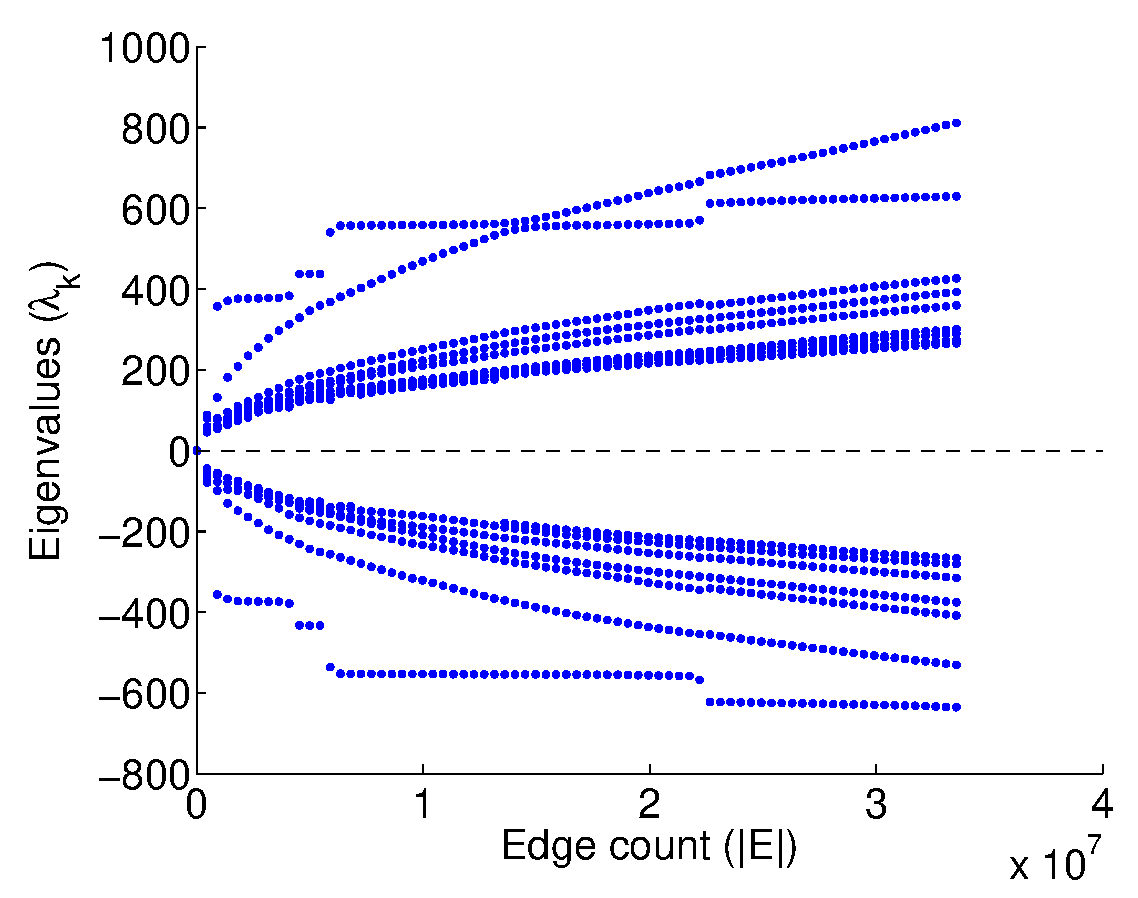
\includegraphics[width=\wTwo\textwidth]{img-st/time.spectrum-flat.sym.wikipedia-growth} &
    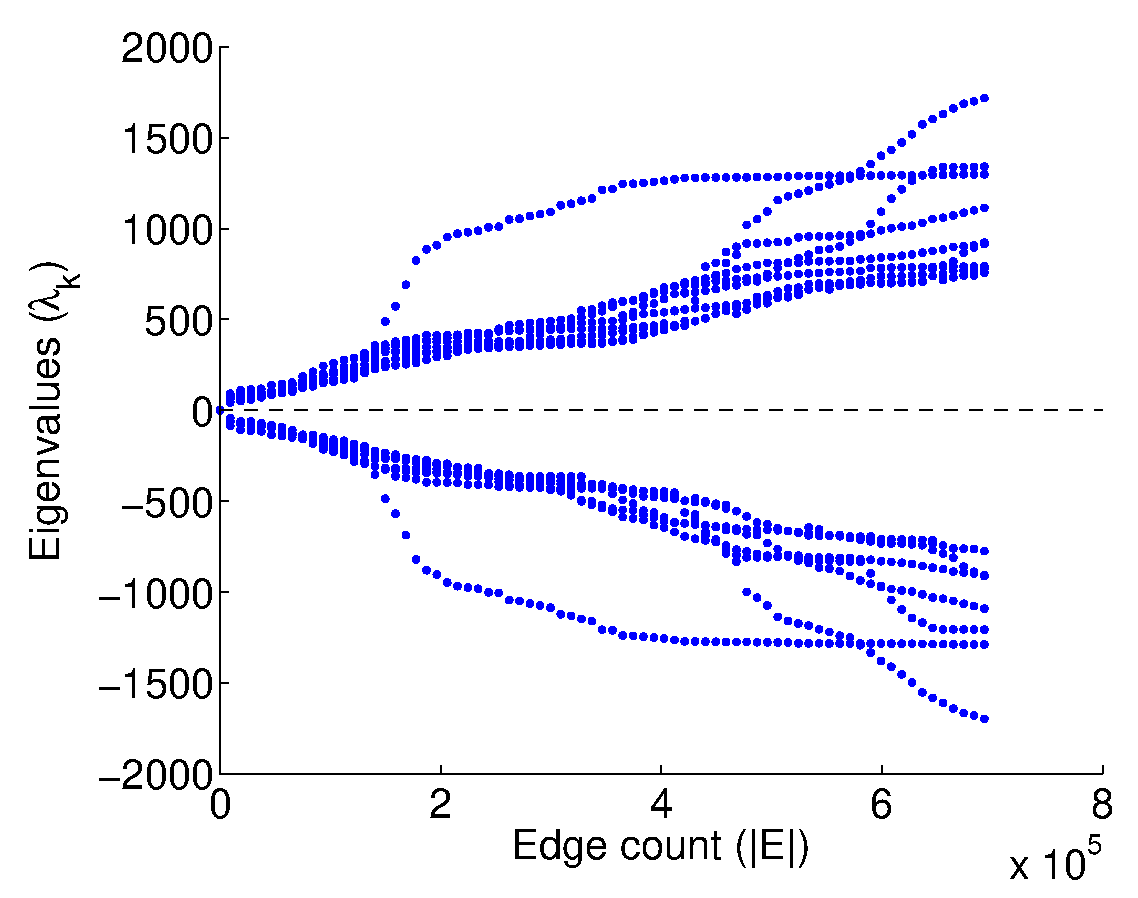
\includegraphics[width=\wTwo\textwidth]{img-st/time.spectrum-flat.sym.facebook-wosn-wall} \\
    Wikipedia hyperlinks (\textsf{WP}) &
    Facebook wall posts (\textsf{Ow}) 
  \end{tabular}
  \caption{
    The spectral evolution of large real-world networks in function of
    time.  At each time, the graphs shows the $\syRank$ dominant
    eigenvalues of the network.
  }
  \label{fig:spectral-evolution}
\end{figure}

A first inspection of these plots suggests that the eigenvalues and
singular values grow over time.   
The observed spectral growth of these networks is sometimes
regular, as in the case of Wikipedia, or irregular, as in the case of
Facebook.  By regular growth, we mean that all eigenvalues grow roughly
with the same speed.  If growth is irregular as for the Facebook
dataset, eigenvalues may overtake each other. 
In many datasets, the observed irregularity is only partial:  Growth of
eigenvalues as a whole does not seem to follow a specific pattern,
although the growth of each individual eigenvalue is smooth. 
This is a first indication of the irregularity of network growth,
and will be a justification later on for extrapolating the eigenvalue
growth into the future. 

We cannot however know at this point that two consecutive eigenvalues with
similar value are related to the same eigenvector.  In fact, any
continuous or small change to a matrix can lead to a small 
change in its spectrum.  
For the spectral evolution model to be valid, spectra must not only
grow, but eigenvectors corresponding to individual eigenvalues must be
stable.  This is inspected in the next test. 

\subsection{Eigenvector Evolution}
\label{sec:eigenvector-evolution}
\index{eigenvector evolution}
To verify whether the spectral evolution model describes the growth of
large, real networks, we compare for each time $t$ the eigenvectors of
$\mathbf A_{t}^{\phantom {\mathrm T}}=\mathbf U_{t}^{\phantom
  {\mathrm T}} \mathbf \Lambda_{t}^{\phantom {\mathrm T}} \mathbf
U_{t}^{\mathrm T}$ with the eigenvectors of $\mathbf
A_{\totaltime}^{\phantom {\mathrm T}}=\mathbf
U_{\totaltime}^{\phantom {\mathrm T}} \mathbf
\Lambda_{\totaltime}^{\phantom {\mathrm T}} \mathbf
U_{\totaltime}^{\mathrm T}$ in Figure~\ref{fig:eigenvector-evolution}.
In these plots, we rely on the eigenvectors to be ordered by their
corresponding eigenvalue.  The plots show one curve for each latent
dimension $k$, showing the number of edges $|E|$ on the X axis and the absolute dot
product of the $k$\textsuperscript{th} eigenvectors at times $t$ and
$\totaltime$ on the Y axis.  The similarity between eigenvectors is
computed as the cosine similarity in the following way:
\begin{align}
  \mathrm{sim}(k,l) &= \left| \mathbf
  (\mathbf U_{\totaltime})_{\bullet k} \cdot \mathbf
  (\mathbf U_{t})_{\bullet l} \right|  
  \label{eq:eigenvector-similarity}
\end{align}
The figure shows, for each $k$, the curve of
$\mathrm{sim}(k,k)$ in function of $t$. 
Eigenvectors corresponding to large eigenvalues are
shown in bright colors and those corresponding to smaller eigenvalues in
light colors.

The eigenvector evolution plots suggest the following interpretation. 
The general trend leaves the eigenvector similarity as measured by the
dot product near one for the lifetime of the network, with 
similarity being higher for those eigenvectors with larger eigenvalues.
In the Facebook network, the similarity of eigenvectors
suddenly drops to zero at specific points in time.  As we will see next,
this is due to eigenvectors changing places in the decomposition, or in other
words, the eigenvalues changing order.  The next test will inspect these
permutations.

\begin{figure}[h!]
  \centering
  \begin{tabular}{ccc}
    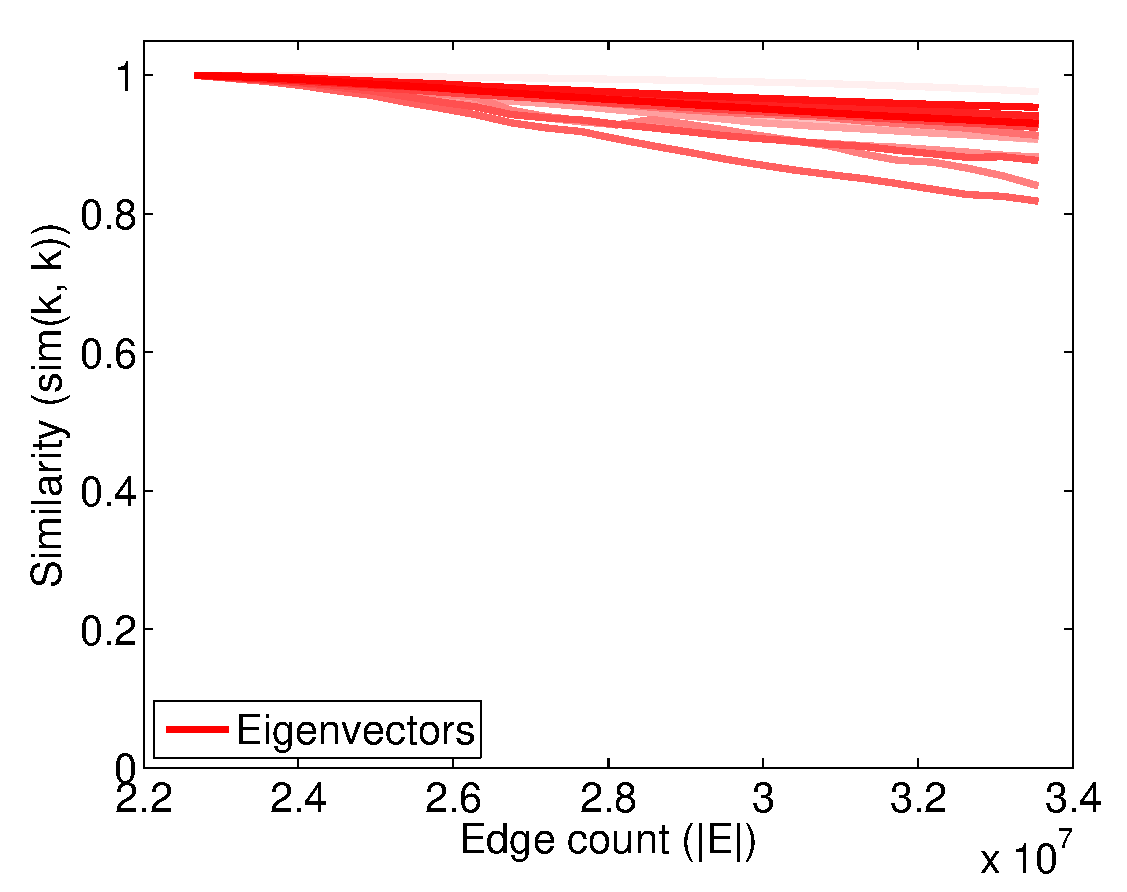
\includegraphics[width=\wTwo\textwidth]{img-st/time.eigenvalue_evolution.sym.wikipedia-growth} &
    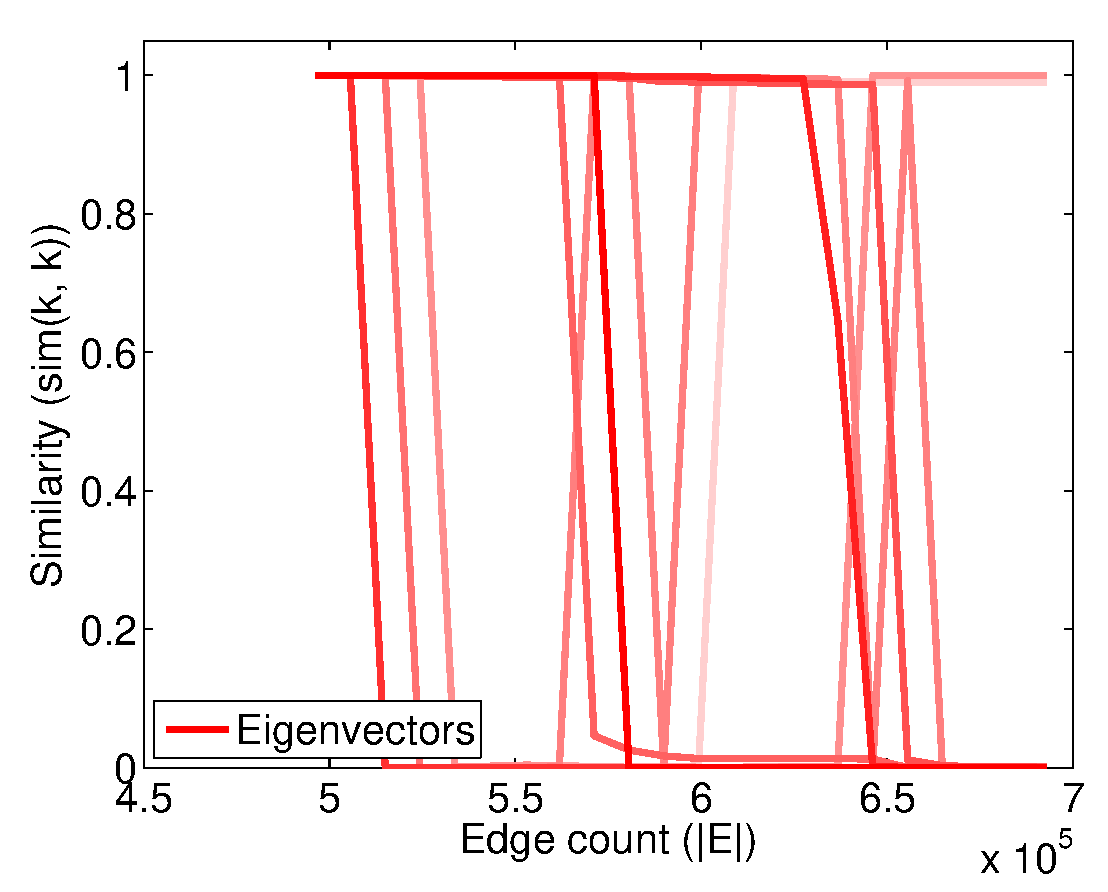
\includegraphics[width=\wTwo\textwidth]{img-st/time.eigenvalue_evolution.sym.facebook-wosn-wall} \\
    Wikipedia hyperlinks (\textsf{WP}) &
    Facebook wall posts (\textsf{Ow}) 
  \end{tabular}
  \caption{
    The evolution of eigenvectors:  The similarity between the
    eigenvectors of the full graph and the eigenvectors of partial
    graphs, by increasing number of missing edges.  Each eigenpair
    is represented by one curve, with brighter colors for dominant latent
    dimensions. 
  }
  \label{fig:eigenvector-evolution}
\end{figure}

\subsection{Eigenvector Stability}
How stable are eigenvectors over time?  To answer this question we
compare the eigenvectors at an intermediary time $t$ with the
eigenvectors at the last known time $T$.  In this test, we 
choose $t$ such that three quarters of all edges are present at time
$t$.  This 75\% split is consistent with the training/test split we
perform in the next chapter.  

We will consider $\mathbf A_{t}$, the adjacency matrix containing all
edges present up to time $t$ and $\mathbf A_{\totaltime}$, the adjacency
matrix of all edges.  We consider the following eigenvalue
decompositions:
\begin{align*}
  \mathbf A_{t}^{\phantom {\mathrm I}}&=\mathbf U_{t}^{\phantom
    {\mathrm I}}\mathbf \Lambda_{t}^{\phantom {\mathrm I}}\mathbf
  U_{t}^{\mathrm T} \\ 
  \mathbf A_{\totaltime}^{\phantom {\mathrm I}}&=\mathbf U_{\totaltime}^{\phantom
    {\mathrm I}}\mathbf \Lambda_{\totaltime}^{\phantom {\mathrm I}}\mathbf
  U_{\totaltime}^{\mathrm T} 
\end{align*}
We then compute $\mathrm{sim}(k,l)$
for all pairs of eigenvector indexes $(k,l)$.  We show the resulting matrices
using white for zero and black for one, and continuous shades in
between in Figure~\ref{fig:permutation}. 
These plots give an indication as to what extent eigenvectors are
preserved over time. 
If all eigenvalues are distinct and network evolution is purely
spectral, the matrices $\mathrm{sim}(k,l)$ are permutation 
matrices.  In addition, they are diagonal when the eigenvalues do
not overtake each other.  
The derivation from a diagonal matrix gives an indication to the
monotony of the underlying spectral transformation. 

Testing the eigenvector stability in this way has one drawback. 
If two eigenvalues are equal, an exchange between
their eigenvectors does not change the matrix.  
This case can be recognized on the eigenvector permutation plots of
Figure~\ref{fig:permutation} as sub-squares containing intermediate
values between zero and one. 
These sub-squares are in fact arbitrary orthogonal matrices, since any
orthogonal basis of the multidimensional eigenspace corresponding to a
multiple eigenvalue can be returned by the eigenvalue decomposition. 
To avoid this, the next test is designed to be robust against such multiple
eigenvalues.   

\begin{figure}[h!]
  \centering 
  \begin{tabular}{ccc}
    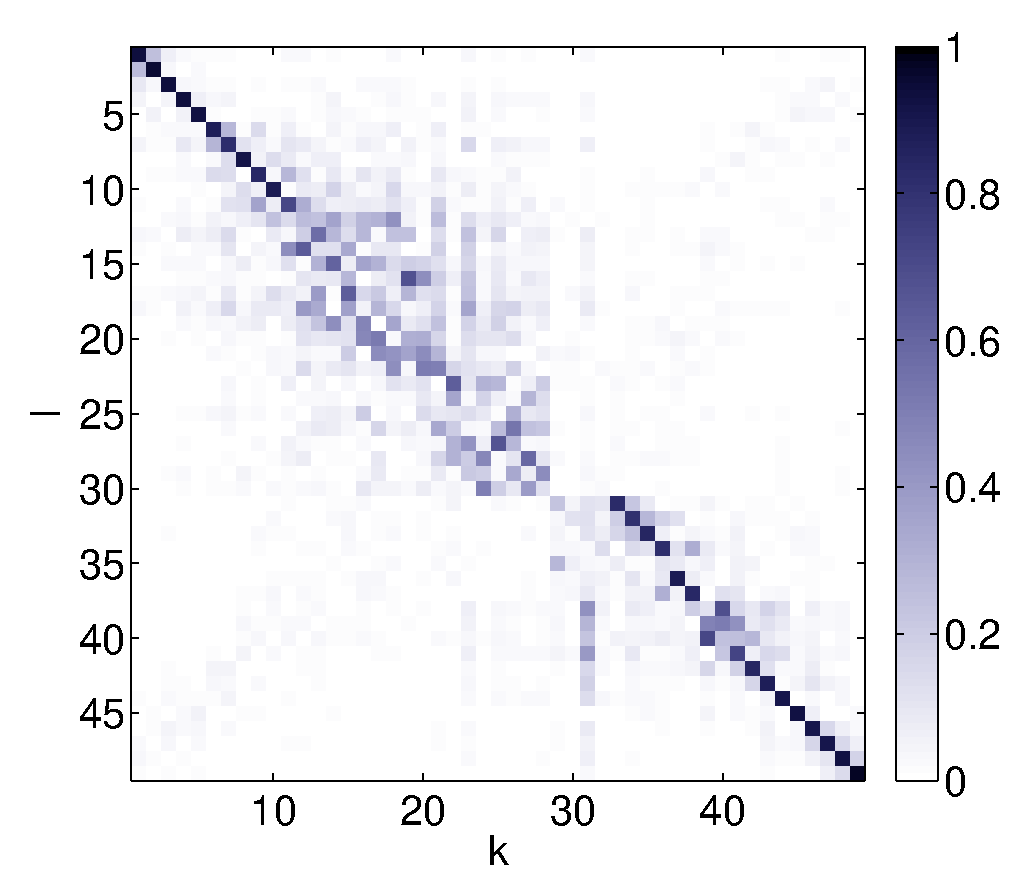
\includegraphics[width=\wTwo\textwidth]{img-st/evol.permutation_map.sym.wikipedia-growth.u} &
    \includegraphics[width=\wTwo\textwidth]{img-st/evol.permutation_map.sym.facebook-wosn-wall.u} \\
    Wikipedia hyperlinks (\textsf{WP}) &
    Facebook wall posts (\textsf{Ow}) 
  \end{tabular}
  \caption{
    The absolute dot product $\mathrm{sim}(k,l)=|\mathbf u_k \cdot
    \mathbf u_l|$ of all eigenvector pairs $(\mathbf u_k,   
    \mathbf u_l)$ at two times $t$ and $T$ in
    network evolution.  These plots show permutation matrices (with zero in
    white and one in black) when the network evolution is purely spectral
    and eigenvalues are simple.  The derivation from a diagonal matrix
    gives an indication to the monotony of the underlying spectral
    transformation.
  }
  \label{fig:permutation}
\end{figure}

\subsection{Spectral Diagonality Test}
\label{sec:spectral-diagonality-test}
\index{diagonality test}
\index{spectral diagonality test}
We now present a test of the amount of change in the eigenvectors which
we call the spectral diagonality test.  If
\begin{align*}
  \mathbf A_{t}^{\phantom{\mathrm{I}}} &= \mathbf
  U_{t}^{\phantom{\mathrm{I}}}\mathbf \Lambda_{t}^{\phantom{\mathrm
      I}} \mathbf U_{t}^{\mathrm T} 
\end{align*}
is the eigenvalue decomposition of a network's adjacency matrix $\mathbf
A_t$ at an intermediate time $t$, then at the final time $T$ it is
assumed to become
\begin{align*}
  \mathbf A_{\totaltime}^{\phantom {\mathrm I}}&=\mathbf U_{t}^{\phantom
    {\mathrm I}} (\mathbf  
  \Lambda_{t}^{\phantom {\mathrm I}}+\mathbf \Delta)\mathbf
  U_{t}^{\mathrm T},
\end{align*}
where $\mathbf \Delta$ should be diagonal.  
Because $\mathbf U_{t}$ has orthogonal columns, 
we can compute the best fit of $\mathbf \Delta$ in a least-squares
sense by
\begin{align}
  \mathbf \Delta &= \mathbf U_{t}^{\mathrm T} (\mathbf
  A_{\totaltime}^{\phantom {\mathrm I}} - \mathbf 
  A_{t}^{\phantom {\mathrm I}})\mathbf U_{t}^{\phantom
    {\mathrm I}}. \label{eq:diagonality}
\end{align}
The resulting matrix $\mathbf \Delta$ is intended to give an indication to what
extent growth is spectral.  Note that in this expression, $\mathbf
A_{\totaltime} - \mathbf A_{t}$ is the adjacency matrix containing all
edges that have appeared between times $t$ and $T$.  It is shown for the
two example networks in Figure~\ref{fig:diagonal}.  We can make
several observations: First, the two matrices are nearly diagonal.  In
fact, we make this observation for all datasets in our collection.
However, the deviation from a diagonal matrix is not equal for all
datasets.  For the Facebook wall posts network (\textsf{Ow}), the matrix
is very near to a diagonal one, and thus the growth is very nearly
spectral.  
For the Wikipedia hyperlink network (\textsf{WP}), the
deviation is larger.  This is a pattern that we observed in almost our
entire collection of datasets: Datasets where multiple edges are allowed
mostly have better spectral growth than those where only simple edges
exist.  A simple explanation can be given for communication networks
such as email networks: In these networks, an edge will appear between
already connected nodes with a certain probability, making growth more
spectral.  In fact, if edges appeared exactly with a frequency
proportional to the number of previously existing edges, the adjacency
matrix would simply be multiplied by a constant, and growth would thus
be spectral.

\begin{figure}[h!]
  \centering
  \begin{tabular}{ccc}
    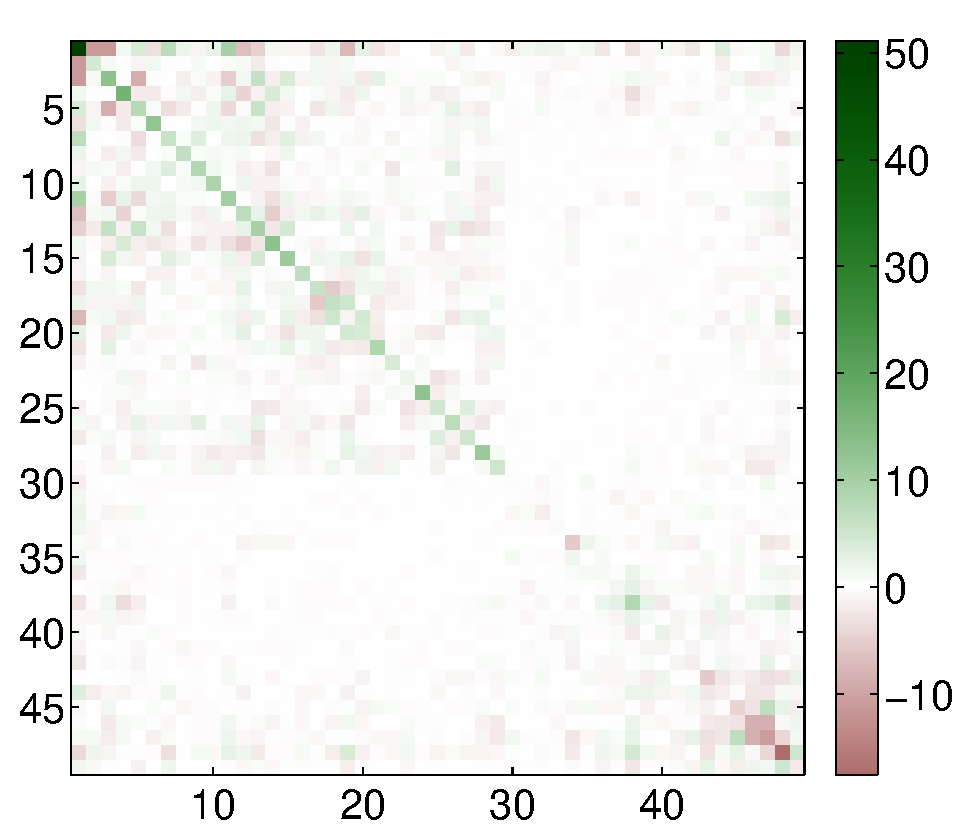
\includegraphics[height=0.40\textwidth]{img-st/comp_permutation_map.symf.wikipedia-growth.a} &
    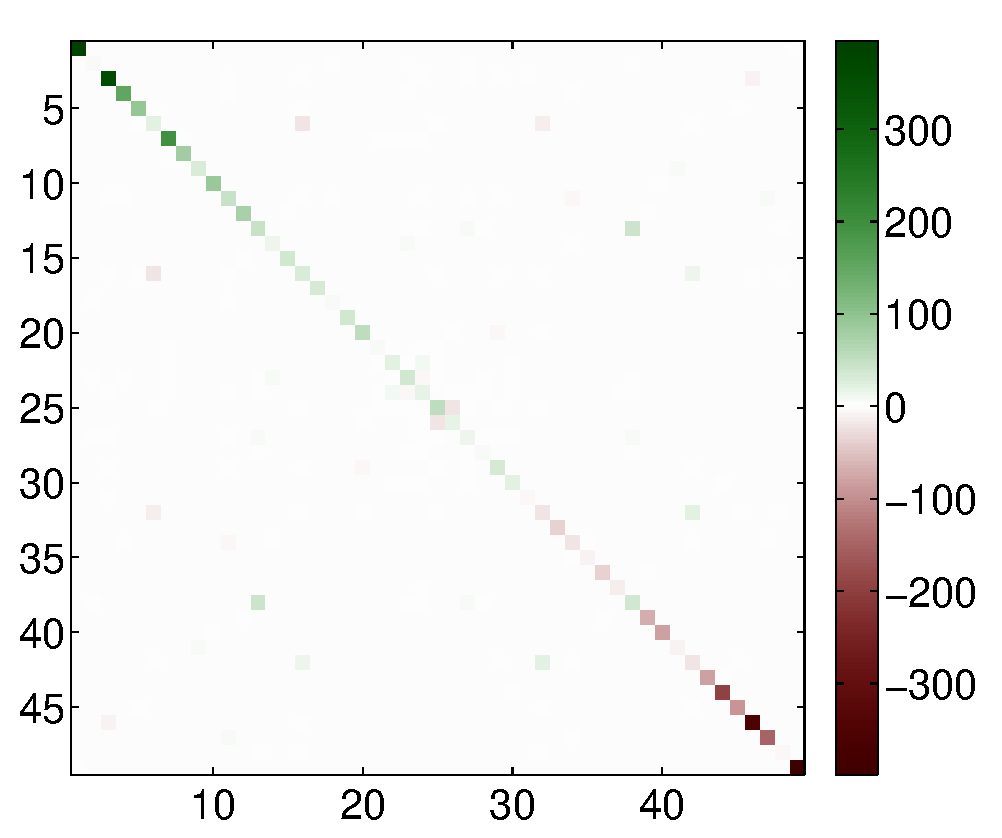
\includegraphics[height=0.40\textwidth]{img-st/comp_permutation_map.symf.facebook-wosn-wall.a} \\
    Wikipedia hyperlinks (\textsf{WP}) &
    Facebook wall posts (\textsf{Ow}) 
  \end{tabular}
  \caption{
    The spectral diagonality test of spectral network evolution.  If network
    evolution is perfectly spectral, the plots show a clean diagonal.
    These plots show the matrix $\mathbf \Delta$ as defined in
    Equation~\ref{eq:diagonality} for the two example datasets. 
  }
  \label{fig:diagonal}
\end{figure}

\section{Generalizing Other Models}
\label{sec:spectral-evolution-model:explanations}
In the previous section, we have observed that the spectral evolution model
holds in many large, real network datasets.  In this section, we will
derive the spectral evolution model from other, more specific graph
growth models. 
As we will see, 
many common graph growth models implicitly rely on spectral growth.  
In other words, the spectral evolution model can be understood as a
generalization of the models presented in this section. 
We will look at these models and study how they can be expressed as a
change of a network's eigenvalue decomposition. 

\subsection{Triangle Closing}
\label{sec:triangle-closing}
\index{triangle closing}
Arguably, the simplest graph growth model is the triangle closing
model.  This model predicts that in a graph, new edges will appear
between nodes that have common neighbors, thus forming (\emph{closing})
triangles.  In social networks, the triangle closing model is known as
the \emph{friend of a friend} model.  The triangle closing model is one
of the easiest to compute nontrivial link prediction methods, 
and is used in practice on very large datasets~\cite{b461}. 

Algebraically, this model can be
expressed as the square $\mathbf A^2$ of the adjacency matrix.  The
matrix $\mathbf A^2$ contains, for each vertex pair $(i,j)$, the number
of common neighbors of $i$ and $j$:
\begin{align}
  (\mathbf A^2)_{ij} &= \sum_k \mathbf A_{ik} \mathbf A_{jk} 
  \label{eq:triangle-closing}
\end{align}
The triangle closing model will thus predict those links that
complete the highest number of triangles.  
The square $\mathbf A^2$ can be expressed using the eigenvalue
decomposition $\mathbf A = \mathbf U \mathbf \Lambda \mathbf U^{\mathrm
  T}$ as
\begin{align*}
  \mathbf A^2 &= \mathbf U \mathbf \Lambda \mathbf U^{\mathrm T} \mathbf U \mathbf
  \Lambda \mathbf U^{\mathrm T} \\
  &= \mathbf U \mathbf \Lambda^2 \mathbf U^{\mathrm T}.
\end{align*}
Here, we use the fact that $\mathbf U$ is orthogonal and thus $\mathbf
U^{\mathrm T} \mathbf U = \mathbf I$.  
As we see, the eigenvalues $\mathbf \Lambda$ are replaced by their
squares $\mathbf \Lambda^2$.  The triangle closing model is thus a
spectral transformation. 
Note that this is also true when using the reduced eigenvalue
decomposition of $\mathbf A$. 
Since $\mathbf \Lambda$ is diagonal, its square can be computed by squaring each
of its diagonal element. 
This equation shows that the triangle closing model $\mathbf A^2$ is a
spectral transformation that corresponds to the real function
$f(\lambda) = \lambda^2$. 

\subsection{Path Counting}
\label{sec:path-counting}
\index{path counting}
The triangle closing model states that edges will appear between
nodes separated by a path of length two.  
In real networks however, we also may
expect edges
to connect two vertices that are more than two edges apart. 
We will thus suppose that new edges complete cycles
of any length, but give lower weight to longer cycles~\cite{b594}. 
The number of paths of a given length $k$ between any two
vertices of a graph can be expressed by the $k$\textsuperscript{th}
power of its adjacency 
matrix $\mathbf A$.  By the same argument as for $\mathbf A^2$,
we can derive that $\mathbf A^k$ is a spectral transformation of
$\mathbf A = \mathbf U \mathbf \Lambda \mathbf U^{\mathrm T}$:
\begin{align*}
  \mathbf A^k &= \mathbf U \mathbf \Lambda^k \mathbf U^{\mathrm T} 
\end{align*}
Thus, the $k$\textsuperscript{th} power of the adjacency matrix
corresponds to the spectral transformation $f(\lambda)=\lambda^k$.
Because matrix multiplication is distributive, a linear combination of
powers of $\mathbf A$ is also a spectral transformation.  In general,
every power series $p(\mathbf A)$ is a spectral transformation:
\begin{align}
  p(\mathbf A) &= \mathbf U p(\mathbf \Lambda) \mathbf U^{\mathrm
    T} \label{eq:path-counting} \\ 
  \alpha \mathbf A^2 + \beta \mathbf A^3 + \gamma \mathbf A^4 + \ldots &=
  \mathbf U (\alpha \mathbf \Lambda^2 + \beta \mathbf \Lambda^3 + \gamma
  \mathbf \Lambda^4 + \ldots  ) \mathbf U^{\mathrm T} \nonumber 
\end{align}
In particular, a power series $p(\mathbf A)$ can be used as a graph growth
model whenever its coefficients are nonnegative and decreasing,
i.e.\ if $\alpha > \beta > \gamma > \ldots \geq 0$.  Power series of this
form have two desirable properties of link prediction functions:
\begin{itemize}
\item Vertices connected by more paths are more likely to connect in the
  future (positivity of the coefficients). 
\item Vertices connected by shorter paths are more likely to connect in
  the future (ordering of the coefficients). 
\end{itemize}
Note that we do not consider the zeroth and first powers of $\mathbf A$:
They only contribute to an additive constant for all node pairs.

\subsection{Graph Kernels}
\label{sec:spectral-evolution-model:explanations:graph-kernels}
\index{graph kernel}
\index{adjacency kernel}
A kernel is a symmetric and positive-semidefinite function of two
variables that denotes a similarity or proximity between objects.  A graph
kernel is defined for a given graph, and denotes the similarity between any
two vertices of that graph.  Many graph kernels exist, most being derived from
specific graph models and typically applied to different
applications~\cite{b137,b152,b155,b156}. 
Since they denote a form of similarity between two vertices, graph
kernels can be used for link prediction.  

Note that the null space of a matrix $\mathbf A$, i.e.\ the set of
vectors $\mathbf x$ such that $\mathbf A \mathbf x=\mathbf 0$, is also called
the \emph{kernel} of $\mathbf A$.  This meaning of the word
\emph{kernel} is not used in this text.  
The phrase \emph{graph kernel} may also refer to a measure of
similarity between individual graphs.  This meaning too is not used
here. 

Many graph kernels are spectral transformations. 
Each of these graph kernels can be described
by a symmetric positive-definite matrix $K(\mathbf A)$ of the same size
as the 
graph's adjacency matrix $\mathbf A=\mathbf U\mathbf \Lambda \mathbf
U^{\mathrm T}$, and that can be written 
as $K(\mathbf A) = \mathbf U F(\mathbf
\Lambda)\mathbf U^{\mathrm T}$ for various functions 
$F(\mathbf \Lambda)$ which apply a real function $f(\lambda)$ to each
eigenvalue in $\mathbf \Lambda$.  In addition to being spectral
transformations, these graph kernels' functions $f(\lambda)$ are convex,
which implies that large eigenvalues grow quicker than smaller
eigenvalues.  By construction, these graph kernels can be computed
from the eigenvalue decomposition of $\mathbf A$. 
Because the graph kernels we describe here are based on the adjacency
matrix $\mathbf A$, we will call them \emph{adjacency kernels}.  Graph
kernels based on other matrices are introduced later in the next
chapter. 

\paragraph{Exponential Kernel}
\index{matrix exponential}
\index{exponential kernel}
The matrix exponential of the adjacency matrix is a graph kernel that
can be used as a link prediction function~\cite{b156}.  A scale
parameter $\alpha$ is typically inserted, to balance the relative weight
of short and long paths. 
\begin{align}
  K_{\mathrm{EXP}}(\mathbf A) &= \exp(\alpha \mathbf A) =
  \sum_{k=0}^\infty \frac {\alpha^k} {k!} \mathbf A^k 
  \label{eq:matrix-exponential}
\end{align}
It corresponds to the spectral transformation $f(\lambda)=e^{\alpha
  \lambda}$.  
When written as a power series, we see that paths are weighted by the
inverse factorial of their length. 
The matrix exponential has nonnegative decreasing coefficients, and is
therefore suited to link prediction. 
The matrix exponential is also called the exponential diffusion
kernel.  

\paragraph{Neumann Kernel}
\index{Neumann kernel}
The Neumann kernel is given by
\begin{align} 
  K_{\textrm{NEU}}(\mathbf A) &= (\mathbf I - \alpha \mathbf A)^{-1} 
  = \sum_{k=0}^\infty \alpha^k \mathbf A^k,
  \label{eq:neumann-kernel}
\end{align}
where $\alpha$ is chosen such that $\alpha^{-1} >
|\lambda_1|$, $|\lambda_1|$ being $\mathbf A$'s largest absolute eigenvalue,
or equivalently the graph's spectral norm~\cite{b263}.  The resulting
spectral transformation is 
$f(\lambda) = 1/(1 - \alpha \lambda)$. 
As the matrix exponential, the Neumann kernel can be written as a
power series with nonnegative decreasing coefficients, and is
therefore a suitable link prediction function.
The Neumann kernel takes its name from the Neumann series 
$\mathbf I + \mathbf A + \mathbf A^2 + \ldots = (\mathbf I - \mathbf 
A)^{-1}$~\cite{b664}, itself named after the German mathematician Carl
Gottfried Neumann. 
In many scientific publications, the Neumann kernel is
called the \emph{von Neumann kernel}.  
We are not aware of how the particle \emph{von} was introduced into this
name, and use the name without \emph{von} in this work.  
The Neumann kernel is sometimes called the Neumann diffusion
kernel~\cite{b152}. 
The link prediction function resulting from the Neumann kernel is
also called the Katz index~\cite{b145}. 

\paragraph{Example}
Using the small synthetic graph from Figure~\ref{fig:syn-graph}, the
following Figure~\ref{fig:syn-kernel} shows the exponential and 
Neumann graph kernels.  For each kernel $\mathrm X \in \{\mathrm{EXP},
\mathrm{NEU}\}$, each vertex $i$ is annotated with the value $K_{\mathrm
  X}(1, i)$, i.e.\ with the kernel's similarity values between each vertex
and vertex~$1$, the leftmost vertex on the graph's representation. 

\begin{figure}[h!]
  \subfigure[The exponential kernel $\exp(\alpha \mathbf A)$]{
    \centerline{
      \xymatrix@C=2cm@R=0.4cm{
        & 3.39  \ar@{-}[dd] \ar@{-}[rd] && 0.71 \ar@{-}[rd] \\
        3.19 \ar@{-}[ru] \ar@{-}[rd] && 2.79 \ar@{-}[dd] \ar@{-}[ru] && 0.15 \\
        & 3.76 \ar@{-}[ru] \ar@{-}[rd] && 0.47 \ar@{-}[rd] \\
        && 1.91 \ar@{-}[ru] && 0.09
      }
    }
  }
  \subfigure[The Neumann kernel $(\mathbf I - \alpha \mathbf A)^{-1}$]{
    \centerline{
      \xymatrix@C=2cm@R=0.4cm{
        & 0.59  \ar@{-}[dd] \ar@{-}[rd] && 0.11 \ar@{-}[rd] \\
        1.31 \ar@{-}[ru] \ar@{-}[rd] && 0.41 \ar@{-}[dd] \ar@{-}[ru] && 0.03 \\
        & 0.65 \ar@{-}[ru] \ar@{-}[rd] && 0.08 \ar@{-}[rd] \\
        && 0.28 \ar@{-}[ru] && 0.02
      }
    }
  }
  \caption{
    The exponential and Neumann kernels applied to the small
    synthetic example network.  The values are the similarity scores
    of each node to the leftmost node (node number~$1$).  The
    parameters are $\alpha =1$ for the exponential kernel and
    $\alpha=0.25$ for the Neumann kernel. 
  }
  \label{fig:syn-kernel}
\end{figure}

\paragraph{Other Graph Kernels}
Some graph kernels such as the commute-time kernel are the spectral
transformation of other 
characteristic graph matrices, such as the graph Laplacian $\mathbf L$
or the normalized
adjacency matrix $\mathbf N$.  These kernels
are however better suited for spectral clustering and less for link
prediction~\cite{b526}. 
We will come back to Laplacian graph kernels in the next chapter, when
applying them to signed graphs. 

\subsection{Rank Reduction}
\label{sec:rank-reduction}
\index{rank reduction}
For large graphs, the eigenvalue and singular value decompositions can
only be computed up to a small rank $\syRank$, in practice not larger than about
100.  The result is an approximation to the adjacency matrix $\mathbf A$
that uses only the $\syRank$ dominant eigenpairs. 
\begin{align}
  R_\syRank (\mathbf A) &= \mathbf U_{\bullet\,(1\ldots\syRank)}^{\phantom{\mathrm I}}
  \mathbf \Lambda_{(1\ldots\syRank)\,(1\ldots\syRank)}^{\phantom{\mathrm
      I}} \mathbf U_{\bullet\,(1\ldots\syRank)}^{\mathrm T}  
  \label{eq:rank-reduction}
\end{align}
where $\mathbf U_{\bullet\,(1\ldots\syRank)}$ and $\mathbf
\Lambda_{(1\ldots\syRank)\,(1\ldots\syRank)}$ are the 
corresponding eigenvector and eigenvalue 
matrices reduced to the largest $\syRank$ eigenvectors by absolute value,
assuming that the diagonal elements $\lambda_k = \mathbf \Lambda_{kk}$
are in 
decreasing order by absolute value, i.e.\ that $|\lambda_1| \geq \ldots
\geq |\lambda_n| $.  
This is the best rank-$\syRank$ approximation of $\mathbf A$ in a
least-squares sense.   

Reduction to a rank $\syRank$ can be interpreted as the spectral
transformation
\begin{align*}
  f(\lambda) &= \left\{ \begin{array}{ll} \lambda & \textnormal{ if }
    |\lambda| \geq |\lambda_\syRank| \\ 0 & \textnormal{ otherwise }
  \end{array} \right. 
\end{align*}
A theoretical ambiguity arises when several
eigenvalues have absolute value $|\lambda_\syRank|$, which is usually ignored
by ordering corresponding eigenvectors arbitrarily.  In practice, the
size of networks and the small value of $\syRank$ make that case very
unlikely. 
The values $\syRank$ we used in experiments for the various datasets are given
in Table~\ref{tab:results-stat} in Appendix~\ref{chap:datasets}.   
This $\syRank$ is chosen to yield a similar, reasonable runtime for each
dataset.  As a result, $\syRank$ is larger for smaller datasets. 

Although rank reduction appears to be a necessary but unwanted
approximation when doing link prediction using spectral methods, some
studies have used rank reduction itself as the link prediction method,
showing that a lower rank may result in more accurate link
prediction~\cite{b166,b140}.  To see how this is possible, consider the
entry $(i,j)$ in the adjacency matrix $\mathbf A$, which is zero if 
$i$ and $j$ are not connected.  
In the matrix $R_\syRank(\mathbf A)$ however, this entry is not zero, and can
be used as a link prediction score for the edge $\{i,j\}$.  
In methods such as latent Dirichlet allocation~\cite{b358} and
nonnegative matrix factorization~\cite{b393} where
a latent model is considered, rank reduction is
also implicit.  
%% Only $\syRank$ eigenpairs of the eigenvalue
%% decomposition can be computed due to the 
%% size of the problem, but computing all $n$ would produce an error-free
%% approximation of the original matrix $\mathbf A$, making any score for
%% non-edges equal to zero. 
In Chapter~\ref{chap:asymmetry}, we will apply rank reduction to
bipartite networks and show that it is equivalent to latent semantic
analysis (LSA) for text datasets. 

\subsection{Latent Preferential Attachment}
\label{sec:latent-preferential-attachment}
\index{latent preferential attachment}
Preferential attachment is a simple link prediction model based on the
idea that the probability of a new link being formed is proportional to
the degrees of the nodes it connects.  This idea can be extended to the
decomposition of a graph's adjacency matrix, resulting in the latent
preferential attachment model, which we describe here.  In this section,
we show that the latent preferential
attachment model is equivalent to the spectral evolution model. 

In a graph with adjacency matrix $\mathbf A$, 
the number                      
of neighbors of a node $i$ is called the degree of $i$ 
and can be written as $d(i) = \sum_j \mathbf A_{ij}$.  
In the preferential attachment model, the probability of an edge
appearing between the vertices $i$ and $j$ is proportional to both
$d(i)$ and $d(j)$.  In other words, links are formed with preference to
nodes that already have a high number of neighbors.  The preferential
attachment model leads to networks were few nodes have many neighbors
and many nodes have few neighbors.  The distributions of node degrees in
such networks can be described by \emph{power laws}, meaning that the
probability that a node has $n$ neighbors is proportional to
$n^{-\gamma}$ for a constant $\gamma > 1$.  Typical values for $\gamma$
are in the range $[2.0,3.0]$, although many other values larger than $1.0$
are observed in practice. 
Such networks are called scale-free networks~\cite{b439} and, as we
established in Section~\ref{sec:scale-free}, most real-world networks
are of this form. 

Now let us consider the eigenvalue decomposition of the adjacency matrix
$ \mathbf A = \mathbf U \mathbf \Lambda \mathbf U^{\mathrm T} $. 
This decomposition can be used to write $\mathbf A$ 
as a sum of rank-one matrices:
\begin{align*}
  \mathbf A &\approx \sum_{k=1}^\syRank \lambda_k^{\phantom{\mathrm I}} \mathbf
  u_k^{\phantom{\mathrm I}} \mathbf u_k^{\mathrm T}  
\end{align*}
where $\syRank$ is the rank of the decomposition, $\lambda_k = \mathbf
\Lambda_{kk}$ 
are the eigenvalues and $\mathbf u_k = \mathbf U_{\bullet k}$ are the
eigenvectors of $\mathbf A$. 
The usual interpretation of a matrix factorization is that each latent
dimension $k$ represents a \emph{topic} in the network.  Then $\mathbf
U_{ik}$ represents the importance of vertex $i$ in topic $k$, and
$\lambda_k$ represents the overall importance of topic $k$. 
Each rank-one matrix $\mathbf A^{(k)} = \lambda_k^{\phantom{\mathrm I}} \mathbf
u_k^{\phantom{\mathrm I}} \mathbf u_k^{\mathrm T}$ can
now be interpreted as the adjacency matrix of a weighted graph.  This
graph $G_k$ will be the complete graph on $n$ vertices, since $\mathbf u_k$ is
typically not sparse when the network is connected.  Therefore, all
information about this graph is 
contained in the weight of the edges.  
Now, assume that preferential attachment is happening in the network,
but restricted to the subgraph $G_k$.  Then the probability of the
edge $\{i,j\}$ appearing will be proportional to $d_k(i) d_k(j)$, where
$d_k(i)$ is the degree of node $i$ in the graph $G_k$.  This degree can
be written as the sum over edge weights in $G_k$:
\begin{align*}
  d_k(i) = \sum_l \mathbf A^{(k)}_{il} 
  = \sum_l \lambda_k \mathbf U_{ik} \mathbf U_{lk} 
  =  \mathbf U_{ik} \lambda_k \sum_l \mathbf U_{lk} 
  \sim \mathbf U_{ik}
\end{align*}
In other words, $d_k(i)$ is proportional to $\mathbf U_{ik}$ only, since
$\lambda_k \sum_l \mathbf U_{lk}$ is independent of $i$. 
Therefore, the preferential attachment value is proportional to the
corresponding entry in $\mathbf A^{(k)}$:
\begin{align*}
  d_k(i) d_k(j) &\sim \mathbf U_{ik} \mathbf U_{jk} 
\end{align*}
These values can be aggregated into a matrix $\mathbf P^{(k)}$ giving
the preferential 
attachment values for all pairs $(i,j)$:
\begin{align*}
  \mathbf P^{(k)} & \sim \mathbf u_k^{\phantom{\mathrm I}} \mathbf u_k^{\mathrm T}
\end{align*}

If we now assume that preferential attachment is happening for each
subgraph $G_k$ separately, with a weight $\varepsilon_k$ depending on the
topic $k$, then the overall preferential attachment prediction can be
written as:
\begin{align*}
  \mathbf P &= \sum_k \varepsilon_k^{\phantom{\mathrm I}} \mathbf
  u_k^{\phantom{\mathrm I}} \mathbf u_k^{\mathrm T} 
\end{align*}
Here, we replace proportionality by equality since the proportionally
constants are absorbed by the constants $\varepsilon_k$.  The matrix $\mathbf
P$ can then be written in the following form, giving its eigenvalue
decomposition:
\begin{align*}
  \mathbf P &= \mathbf U \mathbf E \mathbf U^{\mathrm T} 
\end{align*}
Where $\mathbf E$ is the diagonal matrix containing the individual topic
weights $\mathbf E_{kk} = \varepsilon_k$.  
This prediction matrix is a spectral transformation of the adjacency
matrix $\mathbf A$.  Under this model, network growth can be interpreted
as the replacement of the eigenvalues $\mathbf \Lambda$ by $\mathbf
\Lambda + \mathbf E$:
\begin{align*}
  \mathbf A + \mathbf P &= \mathbf U (\mathbf \Lambda + \mathbf E) \mathbf
  U^{\mathrm T}
\end{align*}

Since the values $\mathbf E$ are not modeled by the latent preferential
attachment model, every spectral transformation can be interpreted as
latent preferential attachment, and thus the latent preferential
attachment model is equivalent to the spectral evolution model. 

\subsection{Irregular Growth}
\index{irregular growth}
We have seen that the spectral evolution model is a generalization of
several graph growth models such as graph kernels.  If these existing
graph growth models already describe the growth of graphs, why do we
need to generalize them?  The answer to that question is that most
graph kernels and other growth models are only valid to a certain
extent.  
By inspecting the growth of actual networks, we can see why these graph
kernels cannot be universally applied for link prediction.
Several cases of observed
irregular spectral evolution are shown in 
Figure~\ref{fig:irregular-evolution}. 

\begin{figure}[h!]
  \centering
  \subfigure[Eigenvalue evolution]{
    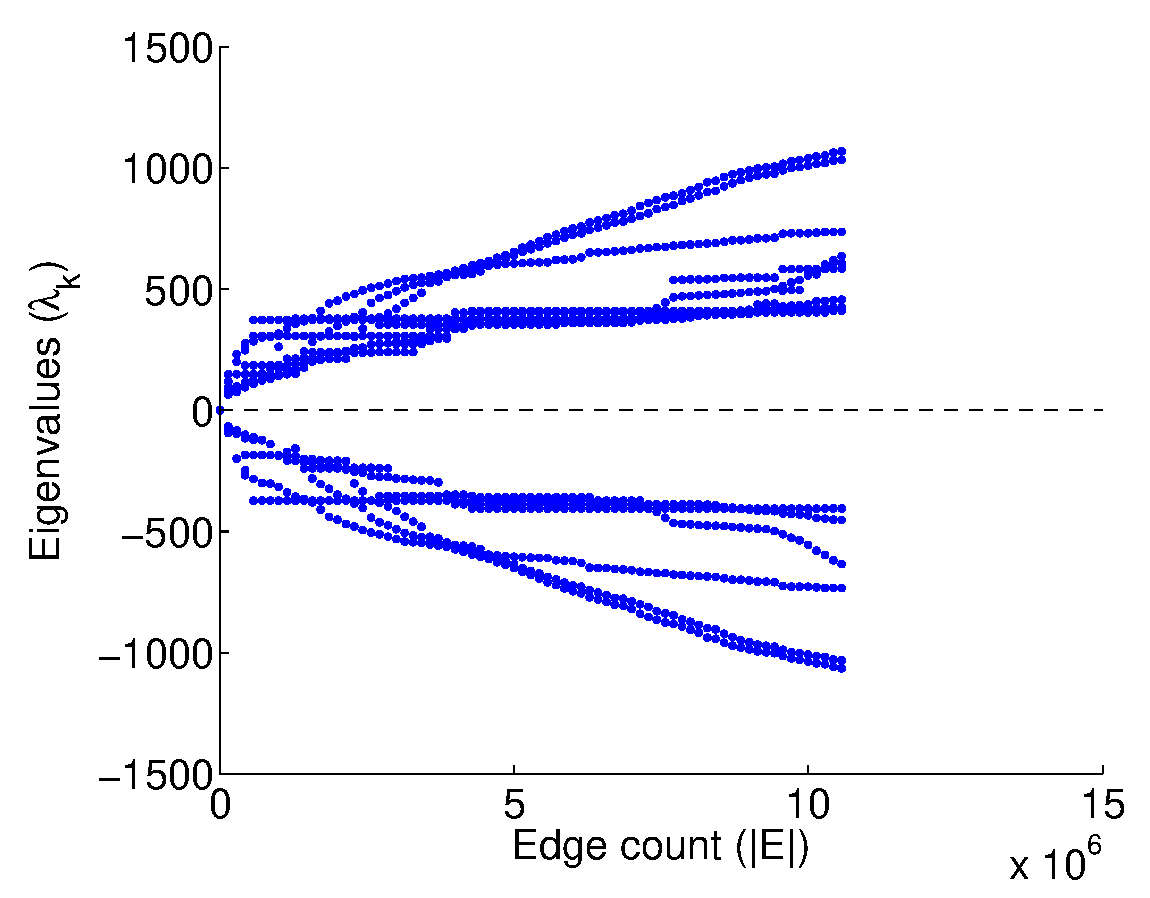
\includegraphics[width=\wTwo\textwidth]{img-st/time.spectrum-flat.sym.munmun_twitterex_at} }
  \subfigure[Spectral diagonality test]{
    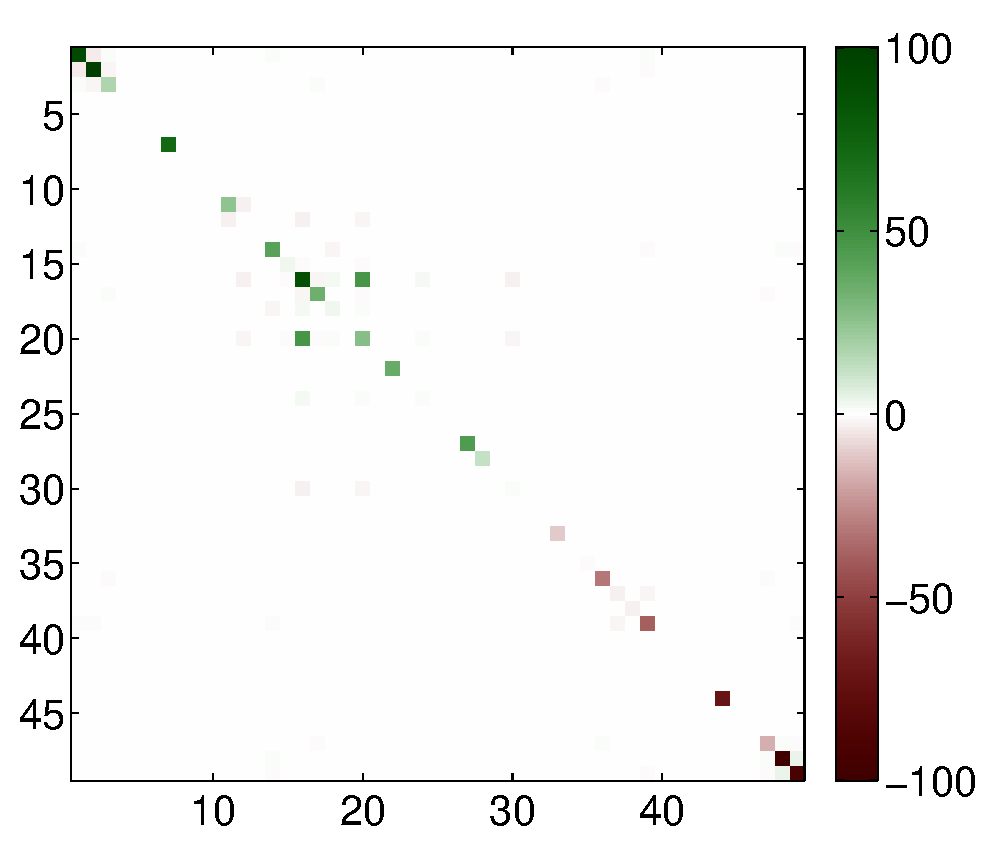
\includegraphics[width=\wTwo\textwidth]{img-st/eval_permutation_map.symf.munmun_twitterex_at.a} }
  \caption{
    Example of irregular but spectral network evolution in the Twitter
    user--user ``@name'' mention network (\textsf{Ws}). 
    (a)~The evolution of the network's eigenvalues over time,
    (b)~The spectral diagonality test applied to a 75\%/25\%
    split of the network. 
    Although the spectral diagonality tests show that growth is spectral in this
    case, this spectral growth is irregular.  The growth of this
    network can thus not be well described by any of the common graph
    kernels. 
  }
  \label{fig:irregular-evolution}
\end{figure}

In these plots, we see that every eigenvalue grows at its own speed.  As
a result, the spectral transformation function $f(\lambda)$ that gives
new eigenvalues as a function of old ones is not regular.
This kind of spectral growth cannot be well described by a function
$f$ that is monotonous like a graph kernel. 
Instead, each eigenvalue is observed to grow at a
specific speed.
Despite this, the evolution of these networks is still spectral. 
It is only the spectral transformation that is irregular. 

From this and other examples, we observe different possible behaviors of
eigenvalue evolution.  Some eigenvalues grow linearly, and others do not
grow.  In the same network, different eigenvalues may grow at different
speeds.  However, we did not encounter any case of an eigenvalue
shrinking over time.  
This behavior may have many explanations, which are usually hard to
guess. 
In most network datasets, nodes are not labeled, and so we cannot
inspect the eigenvectors in question to see which vertices have the
highest value in them. We may however conjecture that stagnating latent
dimensions correspond to communities that die out, or other aspects of
the network that do not grow anymore, for whatever reason. 
Although the reason for each eigenvalue's growth is unknown, it
can still be learned, as we will do later in this chapter.  In fact, these
properties make link prediction algorithms based on spectral
transformations more universal, since they do not rely on
domain-specific knowledge of the network. 

\subsection{Avoided Crossings}
\index{avoided crossing}

As observed in several examples, an eigenvalue can overtake another.
In these cases, our model predicts \emph{crossings} in the spectral
plot.  Looking at 
actual spectra, we however observe something slightly different:  The smaller,
growing eigenvalue slows down growth before it reaches the larger
eigenvalue, and the larger eigenvalue starts growing at about the same
rate.  We observe this behavior in the Wikipedia link network
(\textsf{WP}), as shown in Figure~\ref{fig:overtake-wikipedia}. 

\begin{figure}[h!]
  \centering
  \subfigure[Wikipedia links (\textsf{WP})]{
    \label{fig:overtake-wikipedia}
    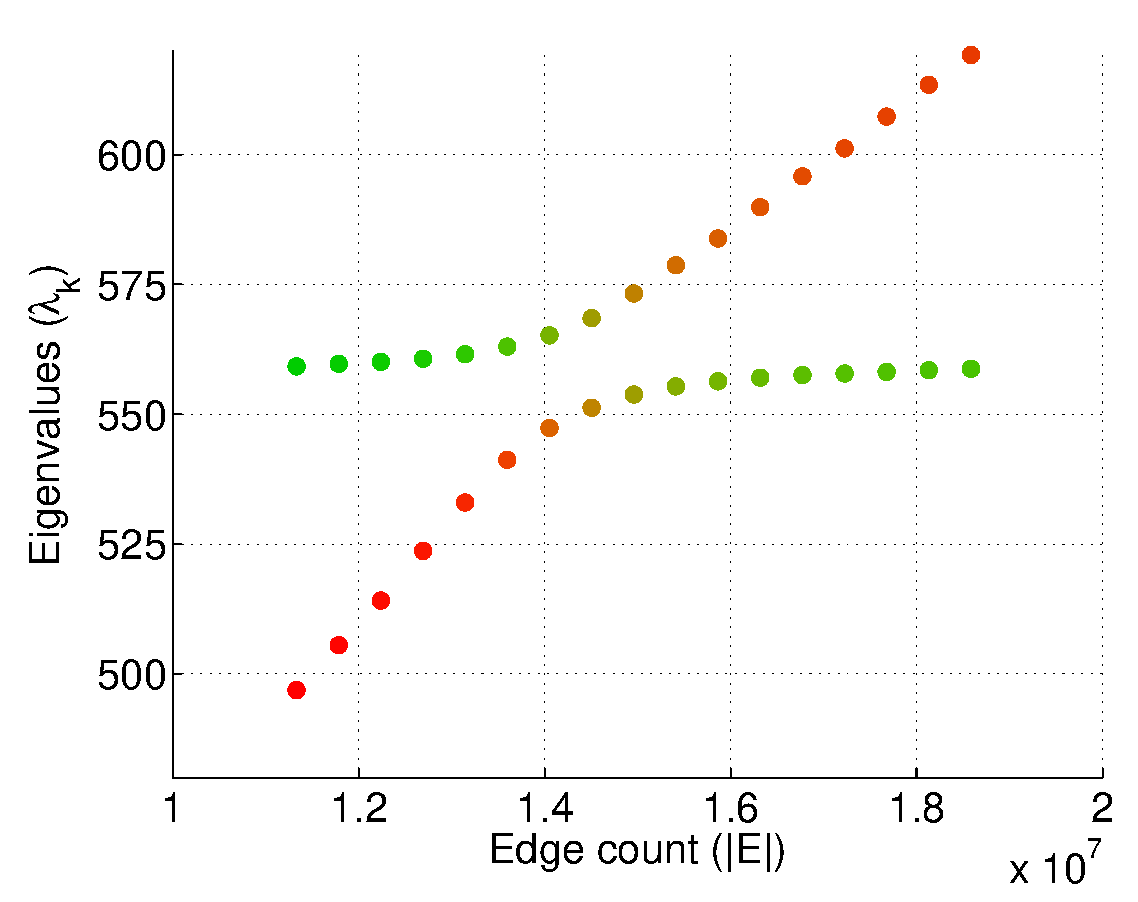
\includegraphics[width=\wTwo\textwidth]{img-st/crossing.sym.wikipedia-growth}}
  \subfigure[Rank-one simulation]{
    \label{fig:overtake-synthetic}
    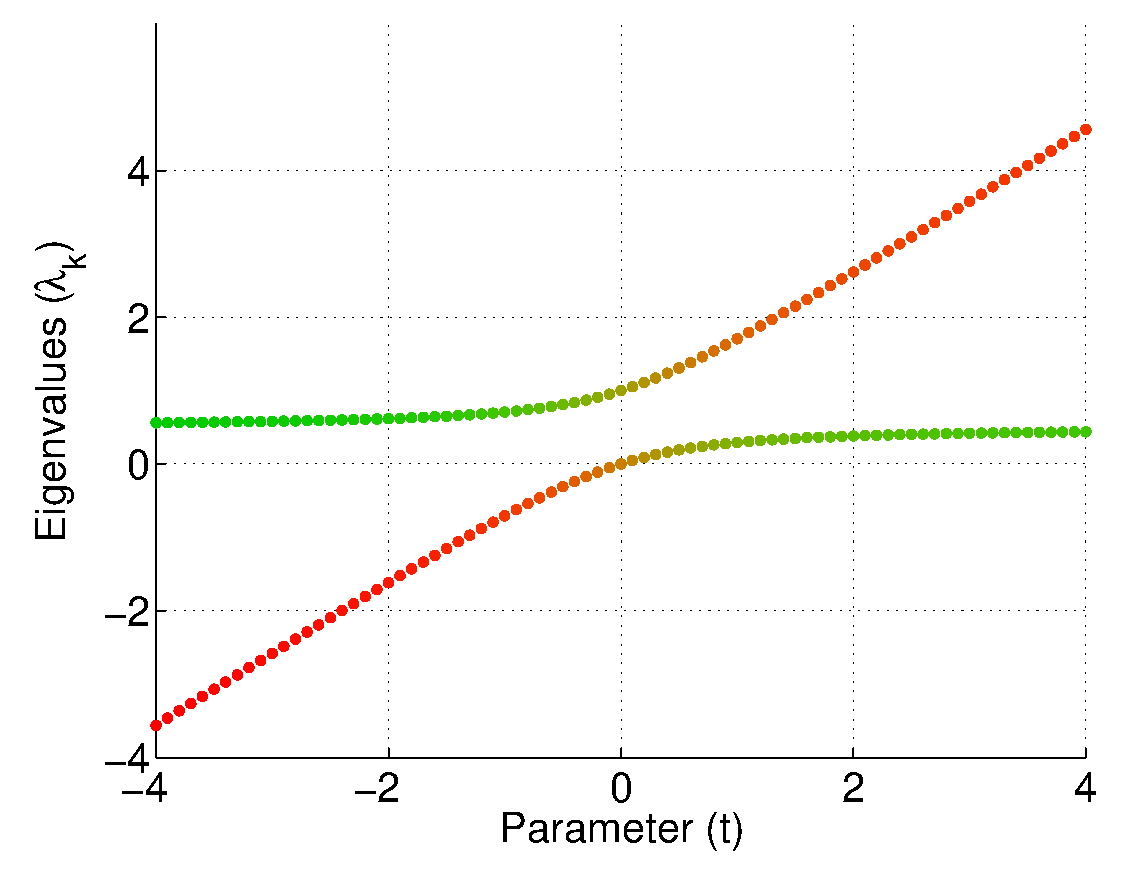
\includegraphics[width=\wTwo\textwidth]{img-st/crossing-col}} 
  \caption                      
      {
        An avoided crossing as observed in the growth of the Wikipedia hyperlink
        network's (\textsf{WP}) two dominant eigenvalues and eigenvectors in~(a), and in
        a rank-one model in~(b).
        The red and green color components of the points denote the
        cosine distance of eigenvectors to initial eigenvectors. 
      }
      \label{fig:overtake}
\end{figure}

This phenomenon is called an \emph{avoided crossing} and can be
explained as follows~\cite[8.5]{b516}.  To simplify the example, we will
assume that certain matrices have rank one, since we are only interested
in individual eigenvalues.  However, the example can be trivially
extended to larger ranks. 
Assume that at a time $t_0$, the adjacency matrix of a network is
$\mathbf A$. 
Now, assume that the growth of the network
around time $t_0$ can be described by a linear function.  Then there is
a matrix $\mathbf B$ such that at time $t$ near $t_0$, the adjacency
matrix of the network at time $t$ is $\mathbf A_t = \mathbf A+(t-t_0)\mathbf B$.  
In the case that $\mathbf A$ and $\mathbf B$ have rank one, the
eigenvalues of $\mathbf A_t$ display an avoided crossing
behavior in most cases. 

Let $\mathbf A=\alpha \mathbf a \mathbf a^{\mathrm T}$ and $\mathbf B = \beta
\mathbf b \mathbf b^{\mathrm T}$.  The matrices $\mathbf A$ and $\mathbf
B$ have as only eigenvectors of nonzero eigenvalue $\mathbf a$ and $\mathbf
b$, respectively. 
Then, $\mathbf a$ and $\mathbf b$ are also eigenvectors of $\mathbf A_t=\mathbf
A+(t-t_0)\mathbf B$ when $\mathbf a$ and $\mathbf 
b$ are collinear or orthogonal.  Otherwise, $\mathbf A_t$ has other
eigenvectors and
an avoided crossing is observed as in
Figure~\ref{fig:overtake-synthetic}. 
Thus, an avoided crossing indicates that a decomposition into
outer products of orthogonal vectors is not the natural representation
for some networks.  If the true decomposition using $\mathbf a$ and
$\mathbf b$ is used,
the crossing would be \emph{unavoided}.  Alternatively, an avoided crossing
may result from a perturbation of orthogonal eigenvectors in the
same manner. 

\section{Control Tests}
\label{sec:spectral-evolution-model:control}
\index{control test}
We have seen in the previous sections that spectral growth is observed
in actual networks, and that it can be explained by several common graph
growth models.  To make sure that the validity of the spectral evolution
model is in itself a 
nontrivial property of real networks, we have to verify that it does
\emph{not} follow from other, random processes.  
We will verify this for two fundamental random processes:  
The random addition of edges, and the random sampling of edges.  To show
that the spectral evolution model is not trivial, it must not be
observed in these trivial models. 
Note that the property of nontriviality is not observed for all graph
characteristics.  Some advanced characteristics such as the modularity,
a measure of the goodness of a node clustering, 
can be observed in the simplest of random graph models, the Erdős--Rényi
model~\cite{b641}. 

Another control tests concerns the choice of the characteristic graph
matrix.  Until now, we have analysed a graph's adjacency matrix.
However, we could equally compute the eigenvalue decomposition of the
Laplacian matrix, and ask whether its eigenvectors are stable.  As we
will see, this is not the case.  The spectral evolution model is only
observed for the adjacency matrix.  This result does not make the
Laplacian matrix useless. As we will see in the next chapter, the
Laplacian matrix can be used to predict links, by learning a mapping
from it to the adjacency matrix.  

\subsection{Random Graph Growth}
\index{random graph growth}
The first random growth model we investigate consists of adding edges 
randomly to a given graph. 
Let $\mathbf A_{t}=\mathbf U \mathbf
\Lambda \mathbf U^{\mathrm T}$ be the adjacency matrix of a network, and $\mathbf
A_{t+1} = \mathbf A_{t}+\mathbf E$ a perturbation of $\mathbf
A_{t}$ where $\left\| \mathbf E \right\|_F=\varepsilon$ is small and
$\mathbf E$ can be thought of as an edge of infinitesimal weight added to
the network.  
The eigenvalue
decomposition of $\mathbf A_{t+1}=\tilde {\mathbf U} \tilde {\mathbf
  \Lambda} \tilde {\mathbf U}^{\mathrm T}$ then has bounds of the
following order: 
\begin{align}
  \left\| \mathbf \Lambda - \tilde {\mathbf \Lambda} \right\|_{\mathrm F} &=
  O(\varepsilon^2) \\  
  \left|\mathbf U_{\bullet k} \cdot \tilde {\mathbf U}_{\bullet
    k}^{\phantom{\mathrm I}}\right| &= O(\varepsilon)
\end{align}
These results can be shown by a perturbation argument~\cite{b528}, and
ultimately can be derived from theorems by
Weyl~\cite{b632} and Wedin~\cite{b633}. 
As a result,
eigenvectors are expected to change faster than eigenvalues for random
additions to the adjacency matrix.  

We verify these theoretical results experimentally using our collection
of datasets.  We use the following methodology:  For each dataset, we
consider the network at time $t$, where 75\% of edges are present.
Then, we add edges randomly until the network has many edges as the
actual network at the final known time $T$.  This gives a new timeline
where the graph grows from 75\% to 100\% of edges.  The actual evolution
and the new, artificial evolution is then compared.  The results are shown
in Figure~\ref{fig:random}.  

\paragraph{Observations}
The first two tests compare the actual and artificial evolution of the
network's eigenvalue and eigenvectors, as done in
Sections~\ref{sec:spectral-evolution}
and~\ref{sec:eigenvector-evolution} on actual networks.  We observe that
in the artificial timeline, neither eigenvalues nor eigenvectors change
significantly (plots~\ref{fig:random:eigenvalue-evolution}
and~\ref{fig:random:eigenvector-evolution}).  The fact that eigenvalues
do not change is explained by the fact that adding edges randomly will,
over long times, only change the eigenvalue with eigenvector $\mathbf
1$, i.e.\ the vector containing only ones.  This means that the dominant
eigenvectors are almost orthogonal to the constant vector, which is
known to be true in high dimensions~\cite{b662}.  The only exception is
for the dominant eigenvector of unsigned networks, which is nonnegative
due to the Perron-Frobenius theorem, and therefore has positive dot
product with the vector $\mathbf 1$.  Additionally, we perform the
spectral diagonality test of Section~\ref{sec:spectral-diagonality-test}
in the plots~\ref{fig:random:random-permutation-map}
and~\ref{fig:random:actual-permutation-map}. The spectral diagonality
tests shows a non-diagonal matrix, implying that artificial growth is
not spectral.  We conclude that spectral growth of networks is not a
consequence of random graph growth, but an inherent property of actual
network growth.

\begin{figure}[h!]
  \centering
  \subfigure[Spectral evolution]{
    \label{fig:random:eigenvalue-evolution}
    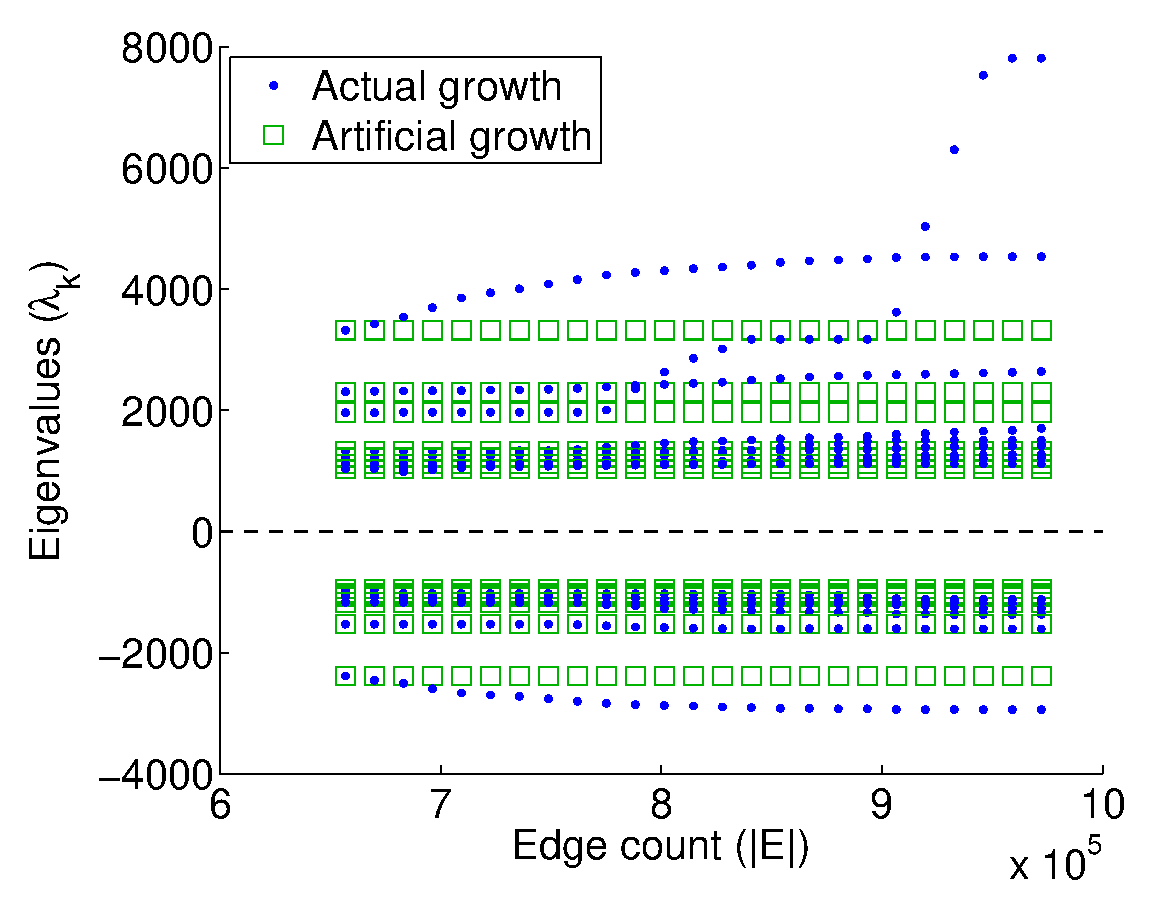
\includegraphics[width=\wTwo\textwidth]{img-st/random.eigenvalue_evolution.enron}
  }
  \subfigure[Eigenvector evolution]{
    \label{fig:random:eigenvector-evolution}
    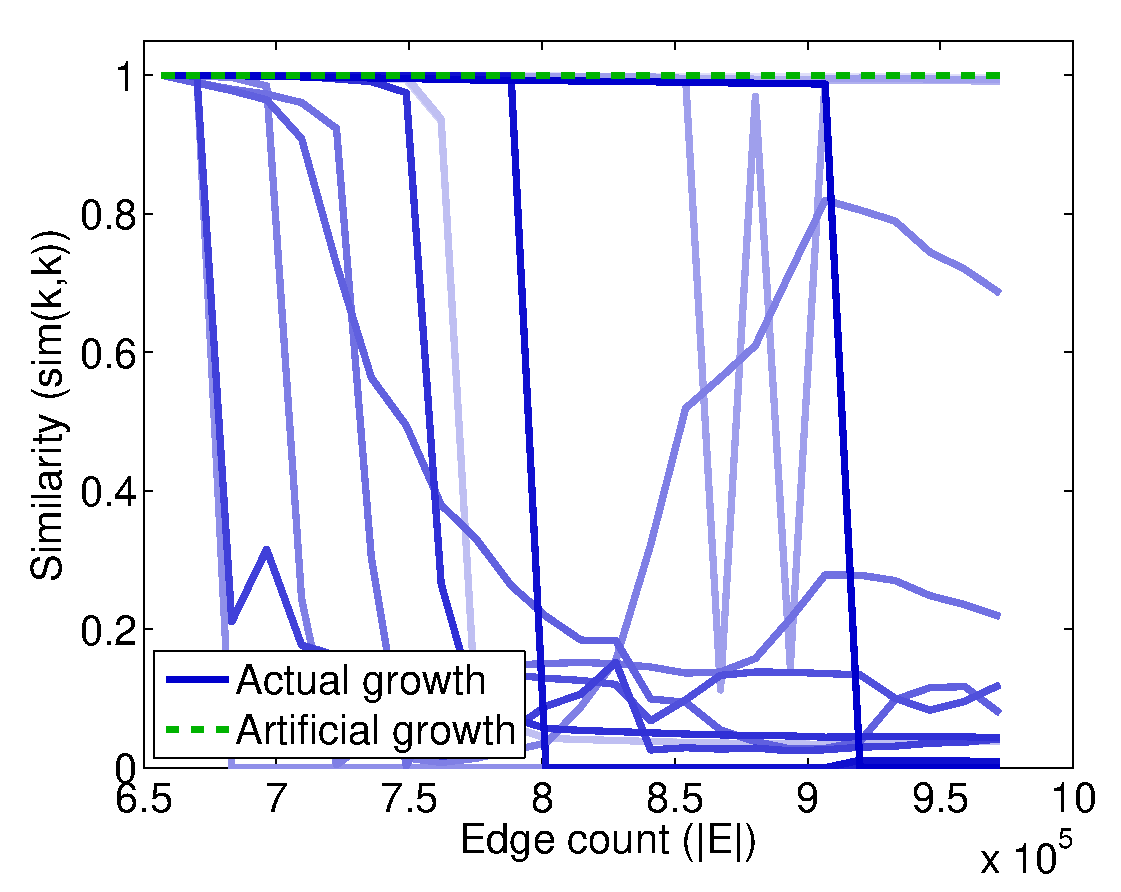
\includegraphics[width=\wTwo\textwidth]{img-st/random.eigenvector_evolution.enron}
  }
  \subfigure[Spectral diagonality test (artificial growth)]{
    \label{fig:random:random-permutation-map}
    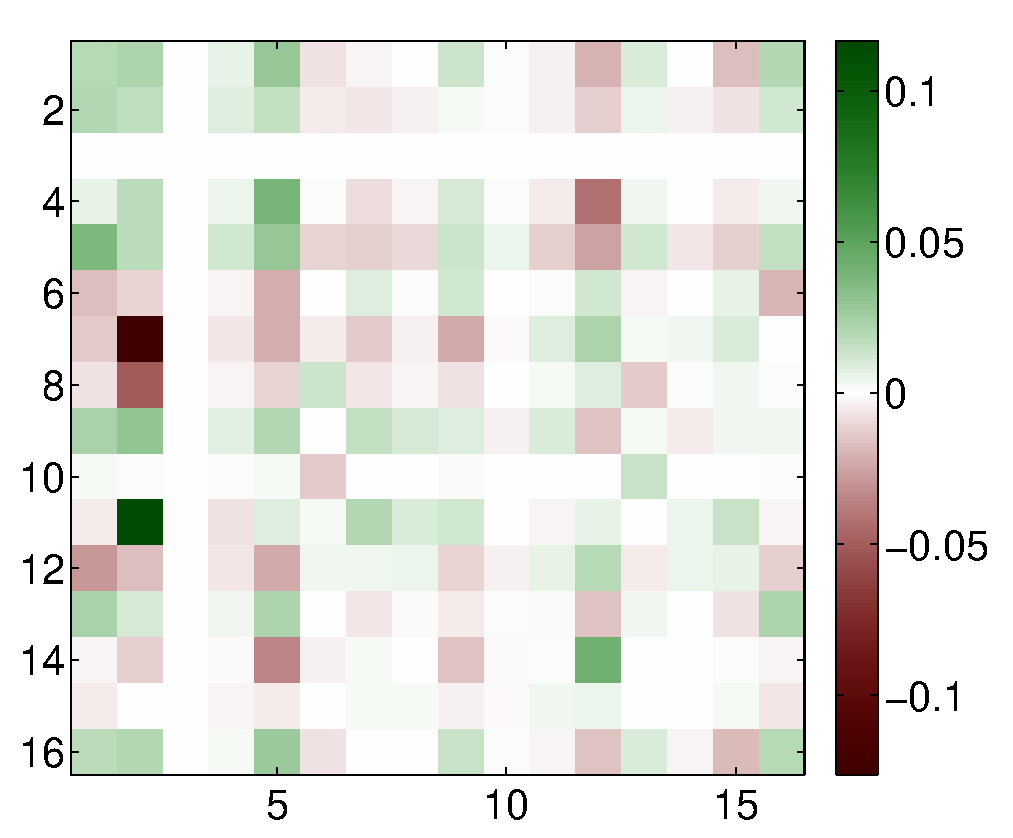
\includegraphics[height=6.3cm]{img-st/random.random_permutation_map.enron}
  }
  \subfigure[Spectral diagonality test (actual growth)]{
    \label{fig:random:actual-permutation-map}
    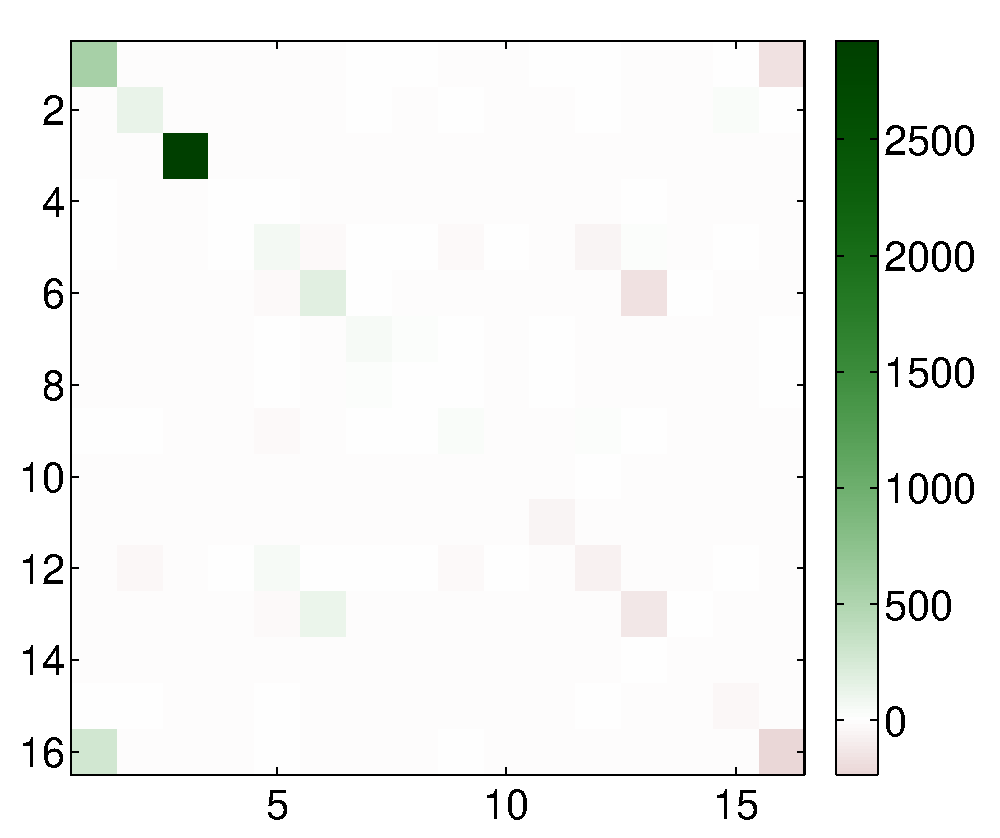
\includegraphics[height=6.3cm]{img-st/random.actual_permutation_map.enron}
  }
  \caption{
    Comparing actual and artificial graph growth.  These plots compare
    the actual growth of the Enron email dataset (\textsf{EN}) with a
    random graph growth model starting at the moment where 75\% of edges
    are present in the dataset. 
  }
  \label{fig:random}
\end{figure}

\subsection{Random Sampling}
\index{random sampling}
In this test, we generate an Erdős--Rényi random graph, and split its
edges randomly into two sets.  We then test how well a spectral
transformation maps one edge set to the other. 

We use the following setup:  Let $G=(V,E)$ be a randomly generated graph
with $|V|=1000$, and the probability of each possible existing edge is chosen
thus that each vertex has on average three neighbors.  
In other words, each edge $\{i,j\}$ is present in the graph with a
probability of $3/(|V|-1)$. 
We make a 75\%/25\% random split into vertex sets $E_{\mathrm a}$ and
$E_{\mathrm b}$ represented by 
the adjacency matrices $\mathbf A_{\mathrm a}$ and $\mathbf A_{\mathrm b}$.
These proportions 
correspond to the training/test split used in the experiments later in this
thesis.  We then compute the reduced eigenvalue decomposition $\mathbf
A_{\mathrm a}=\mathbf U\mathbf \Lambda\mathbf U^{\mathrm T}$
of rank 100. 

Figure~\ref{fig:randspec} shows the spectral diagonality test of
Section~\ref{sec:spectral-diagonality-test} applied to the random graph
$G$ and to the Facebook wall posts network (\textsf{Ow}).  The plots
show the matrix $\mathbf U^{\mathrm T}\mathbf A_{\mathrm b}\mathbf U$. 

\begin{figure}[h!]
  \centering
  \subfigure[Random sampling]{
    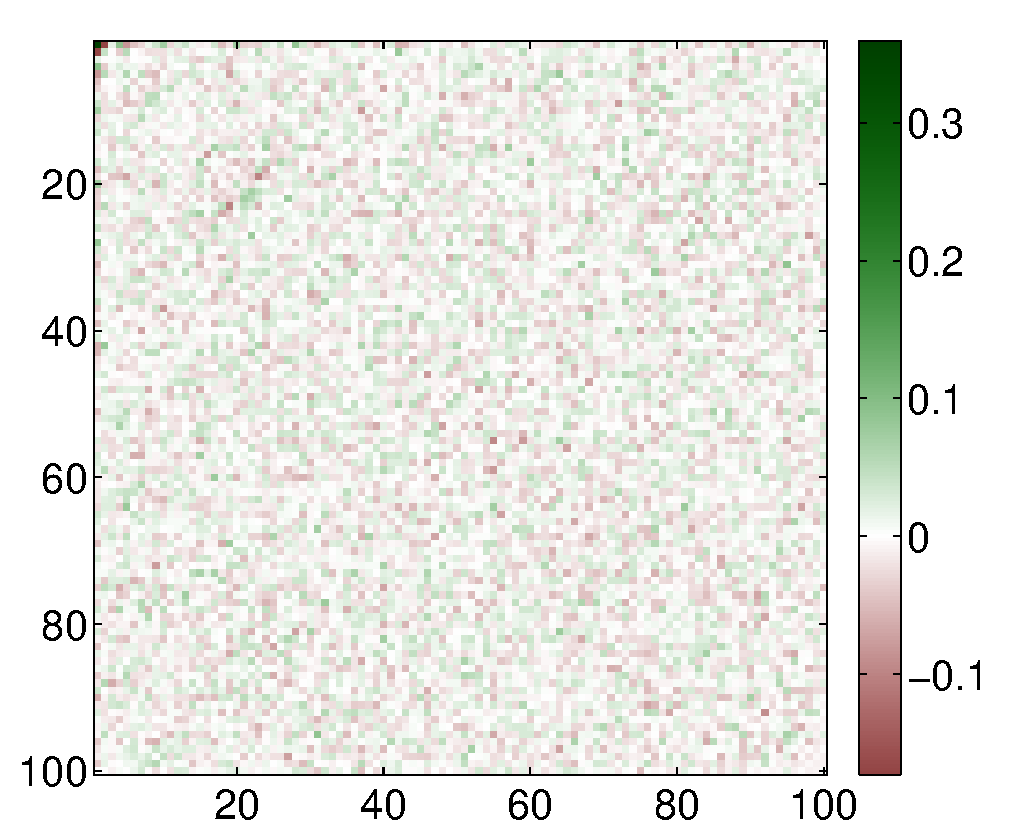
\includegraphics[width=\wTwoMinusLabel\textwidth]{img-eps/randspec}}
  \subfigure[Facebook wall posts (\textsf{Ow})]{
    \includegraphics[width=\wTwoMinusLabel\textwidth]{img-st/comp_permutation_map.symf.facebook-wosn-wall.a}}
  \caption{
    The spectral diagonality test of
    Section~\ref{sec:spectral-diagonality-test} applied to (a)~a random
    sampling from an Erdős--Rényi graph and (b)~the Facebook wall posts
    network (\textsf{Ow}).
    In these tests a diagonal matrix corresponds to a spectral
    transformation implying that only the Facebook network yields a
    spectral transformation. 
  }
  \label{fig:randspec}
\end{figure}

\paragraph{Observations}
In the spectral diagonality test matrix of the random graph (a), there
is clearly only one 
eigenvalue with a significant nonzero value.  This
single eigenpair can be interpreted as a form of preferential
attachment (see Section~\ref{sec:latent-preferential-attachment}), and
is explained by the fact that 
choosing edges at random will return edges adjacent to a node $i$
with probability proportional to the degree of $i$.  Apart from that, no
structure of the original network is preserved spectrally.  
By contrast, the spectral diagonality test for the Facebook wall post
network~(b) is clearly diagonal. 
See also Figure~\ref{fig:diagonal} for more examples of spectral diagonality tests
applied to actual networks. 
We conclude that a spectral transformation of rank greater than one is a
nontrivial emergent property of actual network growth, and cannot be
explained by the Erdős--Rényi random graph model. 

\subsection{Laplacian Spectral Evolution}
\label{sec:laplacian-spectral-evolution}
\index{Laplacian spectral evolution}
We observed previously that the eigenvalue decomposition of a network's
adjacency matrix $\mathbf A$ changes over time in a specific way:  the eigenvalues
grow, and the eigenvectors stay approximately constant.  Having defined
other characteristic graph matrices such as the Laplacian $\mathbf L$
and the normalized adjacency matrix $\mathbf N$, we can ask the question
whether the spectral evolution model can be applied to them. 

Given an unweighted undirected graph $G=(V,E)$ with adjacency matrix
$\mathbf A$, we recall 
that its normalized adjacency matrix $\mathbf N$ and its Laplacian
$\mathbf L$ are given by
\begin{align*}
  \mathbf N &= \mathbf D^{-1/2} \mathbf A \mathbf D^{-1/2} \\
  \mathbf L &= \mathbf D - \mathbf A 
\end{align*}
where $\mathbf D$ is the diagonal degree matrix in which $\mathbf
D_{ii}$ is the degree of vertex $i$.  Due to the relation $\mathbf
I-\mathbf N = \mathbf D^{-1/2} \mathbf L \mathbf D^{-1/2}$, the matrix
$\mathbf N$ is a spectral transformation of the normalized Laplacian
$\mathbf Z = \mathbf D^{-1/2} \mathbf L \mathbf D^{-1/2}$.  For this
reason, what we will say about $\mathbf N$ will also be true for the
normalized Laplacian $\mathbf Z$.  

Figure~\ref{fig:laplacian-evolution} shows the spectral and eigenvector
evolution of the matrices $\mathbf N$ and $\mathbf L$.  In these plots,
we consider the eigenvalue decompositions of the matrices $\mathbf N_t$
and $\mathbf L_t$ at time $t$, for all times $t$:
\begin{align}
  \mathbf N_t &= \mathbf U_t^{\phantom{\mathrm I}} \mathbf
  \Lambda_t^{\phantom{\mathrm I}} \mathbf U_t^{\mathrm T} \\  
  \mathbf L_t &= \mathbf U_t^{\phantom{\mathrm I}} \mathbf
  \Lambda_t^{\phantom{\mathrm I}} \mathbf U_t^{\mathrm T}  
\end{align}
For $\mathbf N$, we compute the top-$\syRank$ eigenvalues and corresponding
eigenvectors. 
For $\mathbf L$, we compute the smallest $\syRank$ eigenvalues and corresponding
eigenvectors.  This is necessary because the matrix $\mathbf L$ is usually
inverted when used (see e.g.\ Section~\ref{sec:laplacian-kernels}). 
The value $\syRank$ depends on the dataset and is chosen to give reasonable
runtimes. Values for $\syRank$ are listed in Appendix~\ref{chap:datasets}. 
We show two kinds of plots:  the spectral evolution as described in
Section~\ref{sec:spectral-evolution} and the eigenvector evolution as
described in Section~\ref{sec:eigenvector-evolution}. 

\paragraph{Observations}
We observe that for both $\mathbf N$ and $\mathbf L$, the eigenvalues
are constant most of the time, and, rarely, they change abruptly.  The
corresponding eigenvectors are not stable, and also change abruptly to
completely different values, indicated by a similarity of zero. 
We conclude that the spectral evolution of $\mathbf N$ and $\mathbf L$
is not smooth, and that the spectral evolution model does not apply to
them.
Even though the matrices $\mathbf N$ and $\mathbf L$ do not change
smoothly, they can be used for link prediction, by applying graph
kernels to them.  This will be explained in
Section~\ref{sec:learning-by-curve-fitting}.  

There is also an algebraic reason why the normalized adjacency and
Laplacian matrices do not grow spectrally.  
Consider the Laplacian $\mathbf L$ of an unweighted, undirected graph
$G=(V,E)$.  Now consider the graph $G'= (V, E\dunion \{i,j\})$,
i.e.\ the graph $G$ to which an edge $\{i,j\}$ has been added.
The Laplacian $\mathbf L'$ of $G'$ is given by 
\begin{align*}
  \mathbf L' &= \mathbf L + \mathbf E,
\end{align*}
where $\mathbf E$ is the matrix defined by $\mathbf E_{ij}=\mathbf
E_{ji}=-1$, $\mathbf E_{ii}=\mathbf E_{jj}=1$ and all other entries of
$\mathbf E$ are zero.  The matrix $\mathbf E$ can be written as 
\begin{align*}
  \mathbf E = \mathbf x \mathbf x^{\mathrm T}
\end{align*}
where the vector $\mathbf x$ is defined by $\mathbf x_i=+1$, $\mathbf
x_j=-1$ and $\mathbf x_k = 0$ for $k\neq i, j$.  Due to a well-known
theorem (see e.g.~\cite[p.~97]{b663}), adding $\alpha \mathbf x \mathbf
x^{\mathrm T}$ to a symmetric matrix will have the following effect on 
the spectrum of the matrix: If $\alpha>0$, then the eigenvalues can only
increase; if $\alpha<0$, the eigenvalues can only decrease. Therefore,
going from $\mathbf L$ to $\mathbf L'$ can only increase the
eigenvalues, not decrease them.  However, known link prediction methods
using the Laplacian as will be described in
Section~\ref{sec:laplacian-kernels} increase the inverse of the
Laplacian eigenvalues and thus would decrease the smallest Laplacian
eigenvalue.  Therefore, these kernels are not consistent with 
a spectral evolution of the Laplacian spectrum.  The same argument is
valid for $\mathbf Z$, making a spectral evolution of $\mathbf N=\mathbf
I - \mathbf Z$ unrealistic.

\begin{figure}[h!]
  \centering
  \begin{tabular}{rccc}
    \begin{sideways}(1) Normalized adjacency matrix $\mathbf N$ \end{sideways} &
    \includegraphics[width=\wTwoMinusLabel\textwidth]{img-st/time.spectrum-flat.sym-n.epinions} &
    \includegraphics[width=\wTwoMinusLabel\textwidth]{img-st/time.eigenvalue_evolution.sym-n.epinions}  \\
    \begin{sideways}(2) Laplacian matrix $\mathbf L$ \end{sideways} &
    \includegraphics[width=\wTwoMinusLabel\textwidth]{img-st/time.spectrum-flat.laps.epinions} &
    \includegraphics[width=\wTwoMinusLabel\textwidth]{img-st/time.eigenvalue_evolution.laps.epinions}  \\
    & (a) Eigenvalue evolution & (b) Eigenvector evolution 
  \end{tabular}
  \caption{
    The spectral evolution in the EU institution email network
    (\textsf{EU}).   
    (1)~the normalized adjacency matrix $\mathbf N$,
    (2)~the Laplacian matrix $\mathbf L$. 
    Two experiments are shown:
    (a)~the spectral evolution as defined in
    Section~\ref{sec:spectral-evolution},
    (b)~the eigenvector evolution as defined in
    Section~\ref{sec:eigenvector-evolution}. 
    In both cases, we observe that the largest eigenvalues of $\mathbf
    N$ and smallest eigenvalues of $\mathbf L$ stay constant. 
  }
  \label{fig:laplacian-evolution}
\end{figure}

\sectionX{Summary}{Summary:  The Spectral Evolution Model} 
The spectral evolution model states that in many real-world
networks, growth can be described by a change of the spectrum, while the
corresponding eigenvectors remain constant.  This assumption is true to
a large extent in most networks we analysed, based on the observation
of the change in eigenvalues and eigenvectors of networks over time.  A
more sophisticated test of the spectral evolution model is what we have
called the spectral diagonality test.  This test measures to what extent
a snapshot of the network at one point can be diagonalized by the
eigenvectors of the same network at another time.  The result is a
matrix that is diagonal exactly when growth is perfectly spectral.
When growth is not spectral, this matrix is not diagonal.  The degree to
which this matrix is diagonal can therefore be used as an indicator of
the spectrality of a network's growth. 
This matrix will be used again in the context of link prediction in the
next chapter, where
we will use it to learn a spectral transformation. 

The fact that the spectral evolution model can be observed in many
networks is not in contradiction to previous results in the literature.
In fact, a 
certain number of known link prediction methods result in network growth
that can be described by spectral transformations.  This class of link
prediction functions includes the triangle closing model, the weighted
path counting model, graph kernels based on adjacency matrix and rank
reduction approaches.  
Another explanation of the spectral evolution model is given by an
extension to the preferential attachment model, which we call the latent
preferential attachment model. 
As we showed, the latent preferential attachment model is equivalent
to the spectral evolution model, under the assumption that a
preferential attachment process happens for each eigenpair
separately.  

To make sure that spectral evolution is a characteristic of real networks and
not an artifact of sampling any network randomly, we performed two
control tests.  By adding edges randomly to an existing network and by
sampling a random network, we could not observe any spectral
growth. This indicates that the spectral evolution model is indeed a
nontrivial property of real-world networks. 

Having confirmed that the spectral evolution model applies to many real
networks,
we can now exploit it to predict links in these networks. 
In the next chapter, we will thus present two new link prediction methods
based on the spectral evolution model.  

\chapter{Learning Spectral Transformations}
\label{chap:learning}
\index{spectral transformation}
In the last chapter, we have observed network growth to follow the
\emph{spectral evolution model}. 
The spectral evolution model that we introduced explained the growth of
networks using the eigenvalue decomposition of their adjacency matrix, 
stating that only the eigenvalues of a network change over time, while
their eigenvectors stay constant. 
In this chapter, this observation is exploited to solve the problem
of link prediction:  Since only the eigenvalues of a network change over
time and not the eigenvectors, it suffices to predict new values for the
eigenvalues. 
We introduce two different methods for doing this.  One uses curve
fitting to learn a function mapping old to new eigenvalues; the
other uses extrapolation of eigenvalues.  

The link prediction problem is fundamental in that it applies to
virtually all types of networks, and can be used to implement
recommender systems and similar applications.  In a social network for
instance, the task of recommending new friends can be viewed, from the
point of view of the recommender system, as the problem of predicting
which edges will appear in the network's future evolution, and
recommending them immediately.  In the physical network of connections
between Internet
hosts, the prediction of new connections is crucial for planning and
optimization.  Similar examples exist for all networks in our
collection, and justify the choice of the link prediction problem as the
main application of the spectral evolution model in this thesis. 

The main idea for link prediction under the spectral evolution model
consists in predicting future values of a network's eigenvalues, and
retaining its eigenvectors. 
The first method we present takes the approach that graph kernels are
correct descriptions of network growth, and learns the parameters of
these graph kernels using curve fitting.  
The second method assumes that the growth of eigenvalues does not follow
any specific pattern, and therefore known link prediction functions
cannot give accurate link 
prediction results.  Instead, the second method extrapolates the change
of eigenvalues into the future for each eigenvalue separately.  
This chapter describes both methods for unweighted, undirected, unipartite
networks.  The case of signed, directed and bipartite networks is
described in the two following chapters. 

We begin the chapter in Section~\ref{sec:link-prediction} by introducing
the link prediction problem formally.  Then, the two new spectral link
prediction methods based on curve fitting and spectral extrapolation are
described in Sections~\ref{sec:learning-by-curve-fitting} 
and~\ref{sec:extrapolation}.  Experimental results for both methods are
given in Section~\ref{sec:learning-experiments}, along with a discussion
of the relative performance of the different graph kernels and of the
different characteristic graph matrices.  Finally, 
Section~\ref{sec:spectral-transformation:related} reviews similar but
unrelated methods used in other areas of data mining on graphs. 

\section{Link Prediction}
\label{sec:link-prediction}
\index{link prediction}
An important class of applications using networks are recommender
systems.  In recommender systems, the task can usually be formulated as
a problem of link prediction. 
In a general sense, \emph{link prediction} denotes the problem 
of predicting links in a network.  
In a broad sense, link prediction is
a very general type of problem that can be formulated on
networks, and is typically hard to solve. 
As examples, recommender systems in the scope of this work are found in
many data mining applications: 
\begin{itemize}
\item A search engine finds documents matching a query.  By modeling
  documents and the words they contain as a bipartite network, 
  matching documents to a query corresponds to finding highly-scored
  links between the query words and documents. 
\item A recommender system can be modeled as a network containing both
  users and items.  Recommendations are then found by predicting links
  from users to items.  The recommender network may connect users and
  items directly such as with ratings, or indirectly, e.g.\ through
  topics, categories, user history, sensors, etc.  
\item Context-aware recommender systems additionally include a context
  for each query, which can be modeled as links between the query and
  the contextual elements.  The task is then to find links between the
  query and entities to recommend. 
\item Rating prediction is a special case of link prediction, where
  edges are weighted.  An important application is collaborative
  filtering, with users rating items. 
\item Finding related items can be achieved by predicting links between items
  connected to a network, even if there are no direct links between the
  items. 
\item To recommend new friends in a social network, some recommender
  systems must find similar nodes in the network. 
  In this case edges are unweighted, and the links
  to be predicted describe the similarity between nodes. 
\item To predict whether a user will like a given movie or not, 
  a recommender system must predict edge weights.
  In this case the network is a bipartite
  rating graph, and missing links in the network have to be predicted. 
\item To predict future interactions, for instance emails or scientific
  coauthorship, link prediction must be performed in a
  network with multiple edges. 
\end{itemize}
For all these problems, there is a network optionally weighted by real
numbers, and the problem consists of predicting future edges.
In particular, we can distinguish the following types of link
prediction:  
\begin{itemize}
\item Given a network, predict which edges will appear 
  (link detection or link completion~\cite{b606}).
\item Given a network and a specific node, predict to which other nodes
  it will connect (recommendation~\cite{b142}).
\item Given a network and a pair of unconnected nodes, determine whether
  it will be connected (link prediction proper~\cite{b256}).
\item Given a weighted network and two unconnected nodes, determine the
  weight of an edge connecting them, knowing that an edge will appear
  between them (collaborative filtering~\cite{b25}, predicting
  trust~\cite{b325}, link sign prediction~\cite{kunegis:slashdot-zoo}). 
\end{itemize}

These problems can be solved by considering link prediction functions:
functions of node pairs returning a numerical score.  The different machine
learning problems given above can then be distinguished by the way these
numbers are 
interpreted, and how they are compared to the actual networks.  Computed
scores for a node pair can be used as prediction values directly, or be
used to find a ranking, which is then compared with the actual known
ranking.

\subsection{Local Link Prediction Methods}
\label{sec:basic-link-prediction-methods}
\index{local link prediction function}
This section describes several simple link prediction methods 
that do not make use of spectral graph theory. 
Due to their simplicity, these methods are very widely used, and will
serve as a baseline against which complex link prediction methods are
evaluated. 
These link prediction functions compute a link prediction score for a
node pair using only information about the immediate neighborhood
of the two nodes.
We will therefore call these functions local \emph{link prediction
  functions}.
All these link prediction functions can be found in~\cite{b256}.   

Let $i$ and $j$ be two nodes in the graph for which a link prediction
score is to be computed.  To compute a link prediction score for the
edge $\{i,j\}$, local link prediction functions depend only on
the neighbors of $i$ and $j$.  
In contrast to this, the spectral link prediction methods described in
the main part of this work take into account the whole network.
In other words, they are global. 

\paragraph{Common Neighbors}
\index{common neighbors}
The number of common neighbors can be used in itself as a link
prediction function~\cite{b256}.  In the example of social
recommendations in a user-user network, this implements the \emph{friend
  of a friend} principle, and is equivalent to
recommending non-friends that have the highest number of common friends:
\begin{align}
  p_{\mathrm{CN}}(i,j) &= |\{ k \mid k \sim i \land k \sim j \}|
  \label{eq:common-neighbors}
\end{align}

The number of common neighbors is a spectral transformation.  It is
equivalent to the triangle closing model described in
Section~\ref{sec:triangle-closing}. 

\paragraph{Preferential Attachment}
\index{preferential attachment}
Taking only the degree of $i$ and $j$ into account for link prediction
leads to the \emph{preferential attachment} model~\cite{b439}, which can
be used as a model for more complex methods such as modularity
kernels~\cite{b401,b413}.
If $d(i)$ is the number of neighbors of node $i$, the preferential
attachment model gives a prediction for an edge between $i$ and $j$ of 
\begin{align}
  p_{\mathrm{PA}}(i,j) &= \frac 1 {2|E|}  d(i) d(j).
  \label{eq:preferential-attachment}
\end{align}
The factor $1/(2|E|)$
normalizes the sum of predictions for a vertex to its degree. 
As we saw in~\ref{sec:latent-preferential-attachment}, a generalization
of the preferential attachment 
model is equivalent to the spectral evolution model. 

\paragraph{Jaccard}
The Jaccard coefficient measures the amount of common neighbors
divided by the number of neighbors of either vertex~\cite{b256}: 
\begin{align}
  p_{\mathrm{JAC}}(i,j) &= \frac {|\{ k \mid k \sim i \land k \sim j \}|}  {|\{ k
    \mid k \sim i \lor k \sim j \}|}  
  \label{eq:jaccard}
\end{align}
The Jaccard coefficient too can be considered a weighted variant of the
common neighbors model. 
In networks with multiple edges, the Jaccard coefficient can be extended
by using multisets in the definition, containing a node $k$ multiple
times when it is connected to $i$ or $j$ multiple times.  

\paragraph{Adamic--Adar}
\index{Adamic--Adar}
The measure of Adamic and Adar~\cite{b475} counts the number of
neighbors, weighted by the inverse logarithm of each neighbor $k$'s
degree $d(k)$: 
\begin{align}
  p_{\mathrm{AA}}(i,j) &= \sum_{k \sim i \wedge k \sim j} \frac 1 {\log(d(k))} 
  \label{eq:adamic-adar}
\end{align}
This can be interpreted as a weighted variant of the common neighbors
model.  

\subsection{Normalization}
\label{sec:normalization}
\index{normalization}
Both local and global link prediction algorithms usually benefit from
normalization.  Normalization consists of applying a
transformation to the data before applying a link prediction
algorithm. 
A typical example of normalization is performed for
rating prediction:  The overall mean rating is subtracted from all
ratings.  After predictions have been computed, the overall mean is
then added to all predicted ratings.  We will call this type of
procedure \emph{additive normalization}.  

In Section~\ref{sec:spectral-graph-theory}, we showed that the
adjacency matrix $\mathbf 
A$ can be replaced by $\mathbf D^{-1/2}\mathbf A\mathbf
D^{-1/2}$ to alleviate the effects of skewed degree distributions. 
This amounts to replacing each entry $\mathbf A_{ij}=1$ by
$1/\sqrt{d(i)d(j)}$.  We will call this procedure \emph{multiplicative 
  normalization}. 
Both types of normalization can be applied to almost all link prediction
algorithms.  In fact, they can even be applied to the trivial link
prediction algorithm that always predicts $1$ or to the trivial rating
prediction algorithm that always predicts $0$:
\begin{itemize}
\item Always predicting $1$ in combination with multiplicative
  normalization leads to the preferential attachment model:  Predict
  $d(i)d(j)$ for the edge $\{i,j\}$.
\item Always predicting $0$ in combination with additive normalization
  leads to the global mean prediction:  Always predict the global mean
  rating. 
\end{itemize}

In this work, additive normalization is always used implicitly for all
weighted networks.  Multiplicative normalization is explicitly used by
using the normalized matrices $\mathbf N$ and $\mathbf M$ instead of
$\mathbf A$ and $\mathbf B$. 

\subsection{Evaluating Link Prediction Methods}
\label{sec:evaluation}
\index{split}
To evaluate a link prediction algorithm, we must know which links
actually appeared in a network and compare them to the links that were
predicted.  In networks where we know the time at which each edge has
appeared, we can split the set of edges by creation time.  We can then
apply a given link prediction algorithm on the training set, use it to
predict links, and compare the predicted links with the test set.

Each of the link prediction algorithms that we introduce in this work
is based on a spectral transformation.  This spectral transformation is
specific to each dataset, and therefore it has to be learned separately
for each dataset.  Thus, we split the training set again by edge
creation time, and use this split to learn a spectral transformation,
which is then applied to the whole test set.  
Finally, the predicted edges are compared with the edges in the test
set. 
Figure~\ref{fig:split} gives a summary of the method we use.

\begin{figure}[h!]
  \centering
  \includegraphics[width=\wOnePointFive\textwidth]{img-pdf/split}
  \caption{
    The three-way split used in all experiments.  The dataset is first split
    into a training and test set by edge creation time.  Then, the
    training set is a again split into a source and target set of
    edges.  Then, a spectral transformation is learned from the source
    to the target set.  This spectral transformation is then applied to
    the training set.  Finally, the predicted edges are compared with
    the edges in the test set. 
  }
  \label{fig:split}
\end{figure}

The split is performed in the following way. First, the training/test
split is made, using 75\% of all edges in the training set and 25\% of
all edges in the test set.  This split is done by edge creation times:
Every edge in the training set is older than every edge in the test
set.  At the time where the split occurs, the network contains all
edges in the training set, and nothing more.  
The training set is then split into a source and target set, also of
sizes 75\% and 25\%. 

Then, the giant connected component is found in the source set, and all
vertices not in the giant component are removed in the source, target
and test sets.  The rationale here is the following:  If an
edge in the test or target set connects two vertices that are not connected by a
path in the
source set, then there is no point in trying to learn this edge.  By
only keeping the giant connected component in the source set, we make
sure that edges in the test and target sets are indirectly connected in
the source
set. This pruning however results in splits that are not
exactly of size 75\%/25\% for all datasets.  If a dataset does not have a
connected component in the source set of at least 10\% of all edges,
then we exclude the dataset from our collection. 

We use the following notation to denote the source, target and test
sets.  In the graph $G=(V,E)$, the set of edges is partitioned as $E =
E_{\mathrm a} \dunion E_{\mathrm b} \dunion E_{\mathrm c}$, where
$E_{\mathrm a}$ is the source set, $E_{\mathrm b}$ is the target set and
$E_{\mathrm c}$ is the test set.  Together, $E_{\mathrm a}$ and
$E_{\mathrm b}$ are the training set.  The adjacency matrix $\mathbf A$
is then decomposed as $\mathbf A = \mathbf A_{\mathrm a} + \mathbf
A_{\mathrm b} + \mathbf A_{\mathrm c}$, where the indexes $\mathrm a,
\mathrm b, \mathrm c$ represent the source, target and test set
respectively.

\subsection{Measuring Link Prediction Accuracy}
\label{sec:map}
\index{mean average precision}
\index{link prediction accuracy}
To compare the experimental results of link prediction algorithms, a
measure of link prediction accuracy has to be used.  Several such
measures are used in the literature, of which we only mention the mean
average precision (MAP)~\cite{b272}, the area under the curve
(AUC)~\cite{b366} and the 
normalized discounted cumulated gain (NDCG)~\cite{b160}.  These measures
of accuracy 
are similar to each other, and our tests indicate that they are
interchangeable for our purpose. Therefore, we will only report
prediction accuracy using a single one of these measures, the mean average
precision, which we now define. 

The mean average precision is based on the ranking implied by link
prediction scores.  In other words, given predicted scores for all
edges, we find the actual edges among them and then their ranking
determines a mean average precision value.  Since the total number of
possible edges is quadratic in the vertex count, this cannot be computed in
practice.  Instead, we generate a \emph{zero test set}, i.e.\ a set of
edges of the same size as the test set, containing only edges not contained
in the original networks.  We call this zero test set $E_{\bar c}$.  

Let $E_{\mathrm c\mathrm{\bar c}} = E_{\mathrm c} \dunion
E_{\mathrm{\bar c}}$ be the total test set of 
edges with $|E_{\mathrm c\mathrm{\bar c}}|=s$. 
For each test edge $e \in E_{\mathrm c\mathrm{\bar c}}$, $\mathbf A_{e}
= (\mathbf A_{\mathrm c})_e$  
is the actual 
edge weight in the test set, and $p_e$ the computed link prediction
value. 
The average precision is then defined in terms of rankings:  Edges
are ranked by their predicted weight, and evaluated by their actual
weight. 
For each edge in $E_{\mathrm c}$, we compute the precision of the results up to
that edge.  The average of these precision values then gives the average
precision.  The average precision is therefore in the range $[0,1]$, and
the value $1$ denotes perfect prediction. 

Let $R(k)$ be the edge of rank $k$ defined such that $p_{R(k)} \leq
p_{R(l)}$ if $k < l$.  Then the average precision is defined as
\begin{align}
  \mathrm{ap}(p) &= \left( \sum_{k=1}^s \left[ \mathbf A_{R(k)}
    \right]_0^1 \right)^{-1} 
  \sum_{k=1}^s \left(\left[ \mathbf A_{R(k)}\right]_0^1 \frac 1 k \sum_{l=1}^k
  \left[ \mathbf A_{R(l)} \right]_0^1 \right), 
\end{align}
where $\left[x\right]_0^1 = 1$ if $x>1/2$ and $\left[x\right]_0^1=0$ otherwise. 

The mean average precision is then given by the mean of average
precision values computed over each node separately~\cite{b521}.  
Let $\mathrm{ap}_i(p)$ be the average precision computed only over all
edges adjacent to vertex $i$.  Then the mean average precision is given
by
\begin{align}
  \mathrm{map}(p) &= \frac 1 {|V|} \sum_{i\in V} \mathrm{ap}_i(p). 
\end{align}
In information retrieval, the average precision is averaged over all
queries.  Here, we consider each vertex in the test set a
query, and consider the prediction of its incident edges a query.  Both
definitions are equivalent. 

\section{Learning by Curve Fitting}
\label{sec:learning-by-curve-fitting}
We now describe a general learning technique for estimating the
parameters of any graph kernel or other link prediction function that
can be expressed as a spectral 
transformation.  This method works by reducing the 
learning problem to a one-dimensional curve-fitting problem.  
As mentioned in
Section~\ref{sec:spectral-evolution-model:explanations}, a
certain number of graph kernels and other link prediction methods 
can be expressed as spectral transformations, 
confirming the spectral evolution model.   
Our contribution in this section is a method for learning the parameters
of these link prediction functions by reducing  
the resulting high-dimensional parameter learning problem to
a one-dimensional curve fitting problem, which can be solved efficiently.
The runtime of this method only depends on the chosen reduced rank, and
is independent of the original network size.  

We show that this generalization is possible under the assumption that
the chosen training and test sets are simultaneously diagonalizable,
an assumption which, as described in
Section~\ref{sec:spectral-evolution-model:explanations}, is implicit in
the spectral evolution model. 
The method presented in this section
can be used to learn the parameters of these kinds of link prediction
functions. 
This includes not only the parameters of graph kernels such as the
matrix exponential, but also the reduced rank in rank reduction methods
and weights used for individual path lengths in path-counting methods. 
Since we reduce the parameter
estimation problem to a one-dimensional curve fitting problem that can
be plotted and inspected visually to compare the different prediction
algorithms, an informed choice can be made about them without having to
evaluate each algorithm on a test set separately.

Let $\mathbf A$ be the adjacency matrix of an undirected, unweighted, unipartite
graph, and $\mathbf A = \mathbf U \mathbf \Lambda \mathbf U^{\mathrm T}$ its
eigenvalue decomposition.  Then the spectral evolution model states that
new links can be predicted by computing a spectral transformation
$F(\mathbf A)= \mathbf U F(\mathbf \Lambda) \mathbf U^{\mathrm T}$.  As
described in Section~\ref{sec:spectral-evolution-model:explanations},
several link prediction functions are of this form, in
particular all graph kernels based on the adjacency matrix such as the
matrix exponential 
$F(\mathbf A) = \exp(\alpha \mathbf A)$.  Most of these graph kernels
have parameters, for instance $\alpha$ for the matrix exponential.  
This section will describe a way to learn these parameters,
and at the same time give a simple method for comparing different graph
kernels in more depth than simply comparing their performances at link
prediction.

Other graph kernels than those presented in
the last chapter 
are not spectral transformations of the adjacency 
matrix $\mathbf A$, but of the Laplacian matrix $\mathbf L$, or the normalized
adjacency matrix~$\mathbf N$.  The method described in this section can
also be applied to these graph kernels, as we will show. 

\subsection{Link Prediction as an Optimization Problem}
Given a graph $G=(V,E)$, we want to find a spectral transformation $F$ that
performs well at link prediction for this particular graph.  
To that end, we divide the set of edges 
$E$ into a training set $E_{\mathrm a}$ and a test set $E_{\mathrm b}$, and then look for a
function $F$ that maps the training set to the test set with minimal error. 

Formally, let $\mathbf A_{\mathrm a}$ and $\mathbf A_{\mathrm b}$ be the
adjacency matrices of the source and target set respectively, such that
$\mathbf A_{\mathrm a}+ \mathbf A_{\mathrm b}$ is the complete known
adjacency matrix of $G$.  In other words, we know $\mathbf A_{\mathrm
  a}$ and want to find a function that maps $\mathbf A_{\mathrm a}$ to
$\mathbf A_{\mathrm b}$.  We will call $\mathbf A_{\mathrm a}$ the
source matrix and $\mathbf A_{\mathrm b}$ the target matrix.  Let
$\mathcal S$ be the set of all spectral transformations from
$\mathbb{R}^{|V|\times |V|}$ to $\mathbb{R}^{|V|\times |V|}$.  The
solution to the following optimization problem then gives the optimal
spectral transformation for the task of predicting the edges in the test
set.
\begin{problem}
  \label{pb:1}
  Let $\mathbf A_{\mathrm a}, \mathbf A_{\mathrm b} \in \mathbb{R}^{|V|\times |V|}$ 
  be two symmetric adjacency matrices over the same vertex set $V$.  
  A spectral transformation that
  maps $\mathbf A_{\mathrm a}$ to $\mathbf A_{\mathrm b}$ with minimal error is given by a
  solution to
  \begin{align}
    \min_F \quad & \left\| F(\mathbf A_{\mathrm a}) - \mathbf A_{\mathrm b} \right\|
    _{\mathrm F}  \label{eq:min-spectral-transformation-error} \\
    \textnormal{s.t.} \quad &  F \in \mathcal S \nonumber
  \end{align}
\end{problem}
The Frobenius norm $\left\|\, \cdot\, \right\|_{\mathrm F}$ corresponds
to the root mean squared error (RMSE) of the mapping from $\mathbf A_{\mathrm a}$
to $\mathbf A_{\mathrm b}$.   
While the root mean squared error is common in link prediction problems,
other error 
measures exist, but give more complex solutions to our problem, making
it impossible to solve the resulting problem efficiently.  We will therefore
restrict ourselves to the Frobenius norm in the rest of the section.  

Problem~\ref{pb:1} can be solved by computing the eigenvalue
decomposition $\mathbf A_{\mathrm a}=\mathbf U\mathbf \Lambda \mathbf U^{\mathrm
  T}$ and using the fact that the Frobenius norm 
is invariant under multiplication by an orthogonal matrix. 
\begin{align}
  &  \big\| F(\mathbf A_{\mathrm a})-\mathbf A_{\mathrm b}\big\|_{\mathrm F} \label{eq:min}  \\
  =& \big\| \mathbf U F(\mathbf \Lambda)\mathbf U^{\mathrm T} - \mathbf
  A_{\mathrm b}\big\|_{\mathrm F} \nonumber \\
  =& \big\| F(\mathbf \Lambda) - \mathbf U^{\mathrm T} \mathbf A_{\mathrm b} \mathbf
  U\big\|_{\mathrm F}  \nonumber
\end{align}
The Frobenius norm in Expression~(\ref{eq:min}) can be decomposed into
the sum of squares of off-diagonal entries of $F(\mathbf
\Lambda)-\mathbf U^{\mathrm T}\mathbf A_{\mathrm b}\mathbf U$, which is independent of $F$,
and into the sum of squares of its diagonal entries.  This leads to the
following least-squares problem equivalent to Problem~\ref{pb:1}:

\begin{problem}
  If $\mathbf U\mathbf \Lambda \mathbf U^{\mathrm T}$ is the eigenvalue
  decomposition of $\mathbf A_{\mathrm a}$, then the solution to Problem~\ref{pb:1} is
  given by $F(\mathbf \Lambda)_{kk}=f(\mathbf \Lambda_{kk})$, where $f(\lambda)$
  is a solution to the following minimization problem.
  \begin{align}
    \min_f \quad & \sum_k \left(f(\mathbf \Lambda_{kk}^{\phantom{\mathrm
        I}}) - \mathbf 
    U^{\mathrm T}_{\bullet
      k}\mathbf A_{\mathrm b}^{\phantom{\mathrm I}}\mathbf U^{\phantom{\mathrm I}}_{\bullet
      k}\right)^2  \label{eq:curve-fitting} 
  \end{align}
\end{problem}
This is a one-dimensional least-squares curve fitting problem of size
$n$.
Since each function $F(\mathbf A_{\mathrm a})$ corresponds to a function
$f(\lambda)$, we can 
choose a link prediction function $F$ and learn its parameters
by inspecting the corresponding curve fitting problem.  
As an example, Figure~\ref{fig:curve-fitting-bare} shows a plot of
$\lambda_k = \mathbf \Lambda_{kk}^{\phantom{\mathrm I}}$ against
$f(\lambda_k) = \mathbf U^{\mathrm
  T}_{\bullet k}\mathbf A_{\mathrm b}^{\phantom{\mathrm I}}\mathbf
U^{\phantom{\mathrm I}}_{\bullet k}$ for the University Rovira
i Virgili email dataset (\textsf{A@}). 

\begin{figure}[h!]              
   \centering
   \includegraphics[width=\wTwo\textwidth]{img-st/curve-bare.symf.arenas-email.a} 
   \caption[
     The one-dimensional least-squares problem used to learn spectral
     transformations by curve fitting.
   ]{
     The one-dimensional least-squares problem used to learn spectral
     transformations by curve fitting.  The values $\lambda_k = \mathbf
     \Lambda_{kk}^{\phantom{\mathrm I}}$ plotted against $f(\lambda_k) =
     \mathbf U^{\mathrm T}_{\bullet k}\mathbf A_{\mathrm
       b}^{\phantom{\mathrm I}}\mathbf U^{\phantom{\mathrm I}}_{\bullet
       k}$ for the University Rovira i Virgili email dataset
     (\textsf{A@}).
   }
   \label{fig:curve-fitting-bare}
\end{figure}

\subsection{Curve Fitting}
\label{sec:curve-fitting}
\index{curve fitting}
We have reduced the general matrix regression
problem~(\ref{eq:min-spectral-transformation-error}) to a 
one-dimensional least-squares curve fitting problem of size $n$.  In
practice, computing the full eigenvalue decomposition $\mathbf A
= \mathbf U \mathbf \Lambda \mathbf U^{\mathrm T}$ is not possible,
first because the decomposition has runtime $O(n^3)$, but also 
because the dense $n
\times n$ matrix $\mathbf U$ would take too much memory to store, 
i.e.\ $O(n^2)$.  
Instead, the
rank-reduced eigenvalue decomposition $\mathbf A \approx \mathbf {\tilde U}
\mathbf {\tilde \Lambda} \mathbf {\tilde U}^{\mathrm T}$ of rank $\syRank$ can be computed.  The
result is that in Equation~(\ref{eq:curve-fitting}), the curve fitting
problem goes only over $\syRank$ points.  Since $\syRank$ is usually much smaller
than $n$ (see Table~\ref{tab:results-stat} in
Appendix~\ref{chap:datasets} for values), this curve 
fitting problem is computationally very easy to solve.  

We now take each spectral link prediction function $F(\mathbf A)$ described in
Section~\ref{sec:spectral-evolution-model:explanations} and, for each
one, derive its underlying real 
function $f(\lambda)$ that applies to every eigenvalue separately.  Most
of the link prediction functions have parameters, e.g.\ the parameter
$\alpha$ in the exponential kernel $\exp(\alpha \mathbf A)$.  These
parameters are kept in the real function.  
Additionally, we insert a multiplicative parameter $\beta > 0$ into
every real function $f(\lambda)$, giving $\beta f(\lambda)$, 
that is to be learned along with the other parameters. 
Although this parameter will not change the relative link prediction
scores and therefore has no influence on the final link prediction
accuracy, including it allows the learned curves to better fit the
observed eigenvalues, and thus results in more sensible values for the
other parameters. 
The resulting functions are summarized in Table~\ref{tab:functions}.  

\begin{table}[h!]
  \centering
  \caption{
    Link prediction functions based on the adjacency matrix and their
    corresponding real functions. 
    The outer multiplicative coefficient $\beta$ (see explanation in the
    text) is not shown, for clarity.
  }
  \label{tab:functions}
  \scalebox{0.93}{
    \begin{tabular}{ l l l l }
      \toprule
      \textbf{Method} & \textbf{Matrix function} & \textbf{Real function}
      \\
      \midrule
      Triangle closing & $\mathbf A^2$ & $f(\lambda) = \lambda^2$ & Eq.~\ref{eq:triangle-closing} \\
      Path counting & $p(\mathbf A) = \sum_{k=0}^\infty \alpha_k \mathbf A^k $ & $f(\lambda) =
      \sum_{k=0}^\infty \alpha_k \lambda^k$ & Eq.~\ref{eq:path-counting} \\ 
      Exponential kernel & $K_{\mathrm{EXP}}(\mathbf A) = \exp(\alpha
      \mathbf A)$ & $f(\lambda) =  e^{\alpha \lambda}$ & Eq.~\ref{eq:matrix-exponential} \\ 
      Neumann kernel & $K_{\mathrm{NEU}}(\mathbf A) = (\mathbf I - \alpha \mathbf A)^{-1}$
      & $f(\lambda) = 1 / (1-\alpha \lambda)$ & Eq.~\ref{eq:neumann-kernel} \\
      Rank reduction & 
      $  R_\syRank (\mathbf A) = \mathbf U_{\bullet\,(1\ldots\syRank)}^{\phantom{\mathrm I}}
      \mathbf \Lambda_{(1\ldots\syRank)\,(1\ldots\syRank)}^{\phantom{\mathrm I}} \mathbf
      U_{\bullet\,(1\ldots\syRank)}^{\mathrm T} $
      &
      $f(\lambda) = \left\{ \begin{array}{ll} \lambda & \textnormal{ if }
        |\lambda| \geq |\lambda_\syRank| \\
        0 & \textnormal{ otherwise } \end{array} \right. $ 
      & Eq.~\ref{eq:rank-reduction} \\
      \bottomrule
    \end{tabular}
  }
\end{table}

Since both $\mathbf \Lambda$ and $\mathbf U^{\mathrm T}\mathbf
A_{\mathrm b}\mathbf U$ are 
available after having computed the eigenvalue decomposition of $\mathbf
A_{\mathrm a}$, the
main computational part of our method lies in the rank-reduced eigenvalue
decomposition of $\mathbf A_{\mathrm a}$.
Additionally, 
the computation of $\mathbf U^{\mathrm T} \mathbf A_{\mathrm b} \mathbf
U$ has runtime complexity 
$O(\syRank |E|)$ and the curve 
fitting runtime is only dependent on $\syRank$.  
By rank reduction, the final least-squares problem has only size $\syRank$,
and the runtime complexity of computing $\mathbf U^{\mathrm T} \mathbf
A_{\mathrm b} \mathbf U$ is 
$O(\syRank n^2)$.  
Since the rank-reduced eigenvalue decomposition of $\mathbf A_{\mathrm a}$ is
computed anyway for spectral link prediction methods and because $r \ll
n \ll n^2$ since $\mathbf A_{\mathrm b}$ is sparse, it follows that
this curve fitting method has only negligible overhead. 

A related idea is to use $\mathbf A_{\mathrm a}+\mathbf A_{\mathrm b}$
instead of $\mathbf 
A_{\mathrm b}$ as the target matrix for optimization, 
in the assumption that a link prediction algorithm should
return high values for known edges.  With this modification, we compute
$\mathbf U^{\mathrm T}(\mathbf A_{\mathrm a} + \mathbf A_{\mathrm
  b})\mathbf U$ instead of 
$\mathbf U^{\mathrm T} \mathbf A_{\mathrm b} \mathbf U$.  Our tests showed that
this variant gave worse results in almost all cases.  We therefore do
not consider this idea any further. 

Finally, we must consider the problem of scaling of eigenvalues.  
The function $F$ is trained on the source matrix $\mathbf A_{\mathrm a}$ and
applied on the target matrix $\mathbf A_{\mathrm b}$.
Since the target adjacency matrix describes more edges than the source
matrix, the corresponding spectra of the two matrices will be different:
The eigenvalues of $\mathbf A_{\mathrm b}$ are
larger than those of $\mathbf A_{\mathrm a}$. Therefore, we propose to
scale the function $F$ in a way that makes it independent of the largest
eigenvalue of the target matrix.  Let $\lambda_{\mathrm a}$ be the
largest absolute eigenvalue of $\mathbf A_{\mathrm a}$ and
$\lambda_{\mathrm b}$ the largest absolute eigenvalue of
$\mathbf A_{\mathrm b}$.  Then the normalized
spectral transformation $F'$ is given by
\begin{align}
  F'(\mathbf \Lambda) &= F\left(\frac {|\lambda_{\mathrm
      a}|}{|\lambda_{\mathrm b}|} \mathbf \Lambda\right).
\end{align}

Figure~\ref{fig:individual-curves} shows our curve fitting method
applied to individual combinations of base matrices and graph kernels for
the University Rovira i Virgili email (\textsf{A@}).  
In this example, a look at the fitted curves suggests that path
counting fits the data well; the matrix exponential fits less well; and
the Neumann kernel and rank reduction fit badly.  We will test in
Section~\ref{sec:learning-experiments} whether this behavior correlates
with high and low prediction accuracy as we would expect. 

\begin{figure}[h!]
  \subfigure[Path counting]{
    \includegraphics[width=\wThree\textwidth]{img-svg/curve.symf.arenas-email.a.poly}} 
  \subfigure[Nonnegative path counting]{
    \includegraphics[width=\wThree\textwidth]{img-svg/curve.symf.arenas-email.a.polyn}} 
  \subfigure[Exponential kernel]{
    \includegraphics[width=\wThree\textwidth]{img-svg/curve.symf.arenas-email.a.exp}} 
  \subfigure[Neumann Kernel]{
    \includegraphics[width=\wThree\textwidth]{img-svg/curve.symf.arenas-email.a.neu}} 
  \subfigure[Rank reduction]{
    \includegraphics[width=\wThree\textwidth]{img-svg/curve.symf.arenas-email.a.dim_lin}} 
  \caption{
    Curve fitting with individual functions of the adjacency matrix $\mathbf
    A$, using the University Rovira i Virgili email network (\textsf{A@}).  
  }
  \label{fig:individual-curves}
\end{figure}

\subsection{Normalized and Laplacian Kernels}
\label{sec:normalized-and-laplacian-kernels}
\index{normalized kernel}
The method of learning a link prediction kernel by curve fitting 
also applies to the Laplacian and normalized adjacency matrices.
Instead of using the non-normalized adjacency 
matrix $\mathbf A$ as the source matrix, we use 
the normalized adjacency matrix $\mathbf N$, 
the Laplacian $\mathbf L$, 
or the normalized Laplacian $\mathbf Z$ 
as the source
matrix.  Here, the matrices $\mathbf N$, $\mathbf L$ and $\mathbf Z$
are understood to be computed
over the source edge set $E_{\mathrm a}$. 

\paragraph{Normalized Kernels}
The exponential and Neumann graph kernels as presented in
Section~\ref{sec:spectral-evolution-model:explanations:graph-kernels}
are spectral transformations of the non-normalized 
adjacency matrix $\mathbf A$.  If instead we use the normalized
adjacency matrix $\mathbf N = \mathbf D^{-1/2} \mathbf A \mathbf
D^{-1/2}$, we arrive at the normalized adjacency graph kernels:
\begin{align}
  K_{\mathrm{EXP}}(\mathbf N) &= \exp(\alpha \mathbf N) 
  = \sum_{k=0}^\infty \frac {\alpha^k}{k!} \mathbf
  N^k \label{eq:normalized-matrix-exponential} \\ 
  K_{\mathrm{NEU}}(\mathbf N) &= (\mathbf I - \alpha \mathbf N)^{-1} 
  = \sum_{k=0}^\infty \alpha^k \mathbf N^k \label{eq:normalized-neumann-kernel}
\end{align}
For the normalized exponential kernel, any positive value can be
used for the parameter $\alpha>0$. 
For the normalized Neumann kernel, the constraint on the parameter
is $0 < \alpha < 1$, because the largest eigenvalue of $\mathbf N$ is
one.  As shown in the next section, the two normalized graph kernels are
both equivalent to graph kernels over the normalized Laplacian matrix
$\mathbf Z = \mathbf D^{-1/2}\mathbf L\mathbf D^{-1/2} = \mathbf I -
\mathbf N$. 

Similarly to the non-normalized case, we can consider path counts on the
graph with normalized edge weights.  The result are power series of the
matrix $\mathbf N$:
\begin{align}
  p(\mathbf N) &= \sum_{k=0}^\infty \alpha_k \mathbf N^k 
  \label{eq:normalized-path-counting} 
\end{align}
A power series of the normalized adjacency matrix $\mathbf N$ in an
unweighted network can be interpreted as the same power series of the
non-normalized adjacency matrix of the weighted network in which each
edge $\{i,j\}$ is given the weight $1/\sqrt{d(i)d(j)}$, with $d(i)$
being the degree of node $i$. 
As in the non-normalized case, good link prediction functions are
expected when the coefficients are
nonnegative and decreasing, i.e.\ $\alpha_0 \geq \alpha_1 \geq \ldots
\geq 0$.  

\paragraph{Laplacian Kernels}
\label{sec:laplacian-kernels}
\index{Laplacian kernel}
Instead of adjacency matrices, we can also use Laplacian matrices to
define graph kernels. 
%% The Laplacian matrix of an undirected, unipartite graph with $n$ vertices
%% is an $n \times n$ 
%% matrix that characterizes the connections between vertices in the graph.
$ \mathbf L = \mathbf D - \mathbf A$ is the non-normalized Laplacian of
the graph, and $\mathbf Z = \mathbf I-\mathbf N = \mathbf
D^{-1/2}\mathbf L\mathbf D^{-1/2}$ is the normalized Laplacian.  The
Laplacian matrices are symmetric and positive-semidefinite.
When the network is unweighted, the multiplicity of eigenvalue zero of
$\mathbf L$ and 
$\mathbf Z$ equals the number of connected components in the network.
The Laplacian matrices are thus singular for nonempty networks.  
The eigenvalues of the normalized Laplacian matrix $\mathbf Z$ lie in
the interval $[0, 2]$. 

Using the eigenvalue decomposition of the Laplacian, several Laplacian
graph kernels can be computed.  
These Laplacian graph kernels are known in the literature 
and have also be used for link prediction~\cite{b155}. 
Spectral transformations of the Laplacian matrix have been used for
semi-supervised learning~\cite{b550}, where they are called transfer
functions.  In this setting, the labels of unlabeled nodes are learned in
a graph where only few nodes are labeled. 
In these studies, only polynomials and stepwise linear
transfer functions are considered. 
These graph kernels are all spectral transformations of the Laplacian,
and therefore they can be learned using curve fitting.  

\paragraph{Moore--Penrose Pseudoinverse}
\label{para:pseudoinverse}
\index{pseudoinverse}
\index{Moore--Penrose pseudoinverse}
Before we introduce commute-time kernels, we first need to introduce the
Moore--Penrose pseudoinverse.  The Moore--Penrose pseudoinverse (or
simply \emph{pseudoinverse}) is a generalization of the matrix inverse
which applies also to matrices that do not have a regular inverse,
including rectangular matrices.  We will only need the 
Moore--Penrose pseudoinverse for square symmetric matrices, and will
therefore only give a definition for these kinds of matrices. 
Recall that a square matrix $\mathbf A$ is invertible when there is a
matrix $\mathbf A^{-1}$ such that
\begin{align*} 
  \mathbf A \mathbf A^{-1} &= \mathbf I. 
\end{align*}
If such an $\mathbf A^{-1}$ exists, then
we have $\mathbf A \mathbf A^{-1} = \mathbf A^{-1} \mathbf A=
\mathbf I$.  Matrices that do not have an inverse are called
\emph{singular}.  While singular matrices do not have an inverse, we can
define a weaker form of inverse called the Moore--Penrose
pseudoinverse.  For any matrix $\mathbf A$, there is a unique $\mathbf
A^+$ such that
\begin{align*}
  \mathbf A \mathbf A^+ \mathbf A &= \mathbf A.
\end{align*}
Such an $\mathbf A^+$ always exists and is called the Moore--Penrose
pseudoinverse of $\mathbf A$.  
If $\mathbf A$ is invertible, then $\mathbf A^+ = \mathbf A^{-1}$. 
If $\mathbf A$ is square and symmetric, then $\mathbf A^+$ can be
expressed as a spectral transformation of $\mathbf A$ as
\begin{align*}
  \mathbf A &= \mathbf U \mathbf \Lambda \mathbf U^{\mathrm T} \\
  \mathbf A^+ &= \mathbf U \mathbf \Lambda^+ \mathbf U^{\mathrm T} 
\end{align*}
where $\mathbf \Lambda^+$ is the diagonal matrix defined by
\begin{align*}
  ( \mathbf \Lambda^+)_{ii} &= 
  \left\{ 
  \begin{array}{ll} \mathbf \Lambda_{ii}^{-1} & \textnormal{ if } \mathbf
    \Lambda_{ii} \neq 0 \\ 0 & \textnormal{ if } \mathbf \Lambda_{ii} =
    0 \end{array} 
  \right. 
\end{align*}
In other words, the Moore--Penrose pseudoinverse is the spectral
transformation that inverts all nonzero eigenvalues and keeps all zero
eigenvalues.  As an example, the Moore--Penrose pseudoinverses of the
zero matrix $\mathbf 0$ and of the identity matrix $\mathbf I$ are
\begin{align*}
  \mathbf 0^+ &= \mathbf 0, \\
  \mathbf I^+ &= \mathbf I^{-1} = \mathbf I. 
\end{align*}
As another example, the Moore--Penrose of the following symmetric
$2\times 2$ matrix is given by its eigenvalue decomposition:
\begin{align*}
  \left[ \begin{array}{cc} 1.6 & 1.2 \\ 1.2 &
      0.9 \end{array}\right]^{\phantom +}
  &=^{\phantom +} \left[ \begin{array}{cc} 0.8 & -0.6 \\ 0.6 & 0.8 \end{array}\right]^{\phantom +}
  \left[ \begin{array}{cc} 2.5 & 0 \\ 0 & 0 \end{array} \right]^{\phantom +}
  \left[ \begin{array}{cc} 0.8 & -0.6 \\ 0.6 &
      0.8 \end{array}\right]^{\mathrm T} \\
  \left[ \begin{array}{cc} 1.6 & 1.2 \\ 1.2 & 0.9 \end{array}\right]^+
  &=^{\phantom +} \left[ \begin{array}{cc} 0.8 & -0.6 \\ 0.6 & 0.8 \end{array}\right]^{\phantom +}
  \left[ \begin{array}{cc} 2.5 & 0 \\ 0 & 0 \end{array} \right]^+
  \left[ \begin{array}{cc} 0.8 & -0.6 \\ 0.6 &
      0.8 \end{array}\right]^{\mathrm T} \\
  &=^{\phantom +} \left[ \begin{array}{cc} 0.8 & -0.6 \\ 0.6 & 0.8 \end{array}\right]^{\phantom +}
  \left[ \begin{array}{cc} 0.4 & 0 \\ 0 & 0 \end{array} \right]^{\phantom +}
  \left[ \begin{array}{cc} 0.8 & -0.6 \\ 0.6 &
      0.8 \end{array}\right]^{\mathrm T} \\
  &=^{\phantom +} \left[ \begin{array}{cc} 0.256 & 0.192 \\ 0.192 & 0.144 \end{array}\right]
\end{align*}

\paragraph{Commute-time Kernels}
\index{commute-time kernel}
\index{normalized commute-time-kernel}
\index{resistance distance}
\index{regularized Laplacian kernel}
\index{normalized regularized Laplacian kernel}
Since the Laplacian matrix is positive-semidefinite, 
its Moore--Penrose pseudoinverse is also
positive-semidefinite and can be used as a graph kernel~\cite{b644}. 
The commute-time kernel can be applied to both the non-normalized
Laplacian $\mathbf L = \mathbf D - \mathbf A$ and to the normalized
Laplacian $\mathbf Z = \mathbf D^{-1/2} \mathbf L \mathbf D^{-1/2}$:
\begin{align}
  K_{\mathrm{COM}}(\mathbf L)  &= \mathbf L^+ \label{eq:commute-time-kernel} \\
  K_{\mathrm{COM}}(\mathbf Z) &= \mathbf
  Z^+  \label{eq:normalized-commute-time-kernel} 
\end{align}
This kernel is sensible because the most significant eigenvectors of the
Laplacian matrices are those with smallest nonzero eigenvalue, which
are mapped to the largest eigenvalues in the Moore--Penrose
pseudoinverse.  The eigenvalue zero however remains at zero with the
Moore--Penrose pseudoinverse.  This is what we want, since the
corresponding eigenvector is the constant vector and would contribute
only a constant term to the link prediction values. 

The pseudoinverse $\mathbf L^+$ can be used to derive a metric:
\begin{align}
  d(i,j) &= (\mathbf L^+)_{ii} + (\mathbf L^+)_{jj} - (\mathbf L^+)_{ij}
  - (\mathbf L^+)_{ji}
  \label{eq:resistance-distance}
\end{align}
This metric has two interpretations.  If the network is interpreted as
an electrical network where each edge is a resistor, this metric gives the
equivalent resistance between any two nodes~\cite{b101}.  The kernel
$\mathbf L^+$ is thus known as the resistance distance kernel and
$\mathbf L$ as the 
Kirchhoff matrix.  When
considering a random walk on the graph $G$, the average commute
time between any two node equals the resistance distance.  
The equivalence between the two formalisms is studied in~\cite{b19}. 
Note that the resistance defined in
Equation~\ref{eq:resistance-distance} can be interpreted as a squared
Euclidean distance in the following way:  If $\mathbf L = \mathbf U
\mathbf \Lambda \mathbf U^{\mathrm T}$ is the eigenvalue decomposition
of the matrix $\mathbf L$, then let $\mathbf W = \mathbf U 
(\mathbf \Lambda^+)^{1/2}$.  Then, interpret each row $\mathbf W_{i\bullet}$ of
$\mathbf W$ as the coordinate of vertex $i$ in a space of dimension
$n$. Then, the squared Euclidean distance between vertices in this
spaces equals the resistance distance.  For every pair $(i,j)$, we have: 
\begin{align*}
  (\mathbf W_{i\bullet} - \mathbf W_{j\bullet})^2 
  &= \mathbf W_{i\bullet}^{\phantom{\mathrm I}} \mathbf
  W_{i\bullet}^{\mathrm T} 
  + \mathbf W_{j\bullet}^{\phantom{\mathrm I}} \mathbf W_{j\bullet}^{\mathrm T} 
  - \mathbf W_{i\bullet}^{\phantom{\mathrm I}} \mathbf
  W_{j\bullet}^{\mathrm T} 
  - \mathbf W_{j\bullet}^{\phantom{\mathrm I}} \mathbf
  W_{i\bullet}^{\mathrm T} \\ 
  &= \mathbf U_{i\bullet}^{\phantom{\mathrm I}} \mathbf \Lambda^+ \mathbf U_{i\bullet}^{\mathrm T}
  +  \mathbf U_{j\bullet}^{\phantom{\mathrm I}} \mathbf \Lambda^+ \mathbf U_{j\bullet}^{\mathrm T}
  -  \mathbf U_{i\bullet}^{\phantom{\mathrm I}} \mathbf \Lambda^+ \mathbf U_{j\bullet}^{\mathrm T}
  -  \mathbf U_{j\bullet}^{\phantom{\mathrm I}} \mathbf \Lambda^+ \mathbf
  U_{i\bullet}^{\mathrm T} \\
  &= (\mathbf L^+)_{ii} + (\mathbf L^+)_{jj} - (\mathbf L^+)_{ij} -
  (\mathbf L^+)_{ji}  \\
  &= d(i,j)
\end{align*}

To impose smoothness on Laplacian graph kernels, they can be regularized
by adjusting specific spectral transformations to them~\cite{b155}.  In
particular, we will call the following kernels the regularized Laplacian
kernels: 
\begin{align}
  K_{\mathrm{REG}}(\mathbf L)  &= (\mathbf I+\alpha \mathbf L)^{-1} 
  = \sum_{k=0}^\infty (-\alpha)^k\mathbf L^k 
  \label{eq:regularized-laplacian-kernel} \\
  K_{\mathrm{REG}}(\mathbf Z) &= (\mathbf I+\alpha \mathbf Z)^{-1} 
  = \sum_{k=0}^\infty (-\alpha)^k\mathbf Z^k
  \label{eq:normalized-regularized-laplacian-kernel} 
\end{align}
The parameter $\alpha$ must be larger than zero in both cases. 
For the infinite series representation to be defined, $\alpha$ must be
less than the inverted largest eigenvalue of $\mathbf L$ and $\mathbf
Z$, i.e.\ $\alpha < 1/2$ for $\mathbf Z$.  Otherwise, the kernel is
still defined, but does not have a series expansion. 
The regularized Laplacian kernels characterize the proximity of two
vertices by the number of ways they can be connected by random
forests~\cite{b190}.  For this reason, they are also called random forest
kernels. 
The normalized regularized Laplacian is equivalent to the normalized 
Neumann kernel by noting that $(\mathbf I+\alpha \mathbf Z)^{-1}
=(1+\alpha)(\mathbf I-\alpha\mathbf N)^{-1}$.  This is true because we
have $\mathbf Z=\mathbf D^{-1/2} \mathbf L \mathbf D^{-1/2} = \mathbf
D^{-1/2} (\mathbf D - \mathbf A)\mathbf D^{-1/2}=\mathbf I-\mathbf N$. 

\paragraph{Heat Diffusion}
\index{heat diffusion}
\index{normalized heat diffusion}
By considering a process of heat diffusion on the network, a Laplacian heat
diffusion kernel can be derived~\cite{b137}: 
\begin{align}
  K_{\mathrm{HEAT}}(\mathbf L)  &= \exp(-\alpha \mathbf
  L) \label{eq:heat-diffusion} \\ 
  K_{\mathrm{HEAT}}(\mathbf Z) &= \exp(-\alpha \mathbf Z) 
  \label{eq:normalized-heat-diffusion}
\end{align}
The normalized heat diffusion kernel is equivalent to the normalized exponential
kernel given by $\exp(-\alpha \mathbf Z) = e^{-\alpha} \exp(\alpha \mathbf
N)$ \cite{b155}.
The heat diffusion kernel is also known as the Laplacian exponential
diffusion kernel~\cite{b152}. 

The normalized Laplacian can be derived from the normalized
adjacency matrix by the spectral transformation $\mathbf Z =
F(\mathbf N)=\mathbf I -\mathbf N$ corresponding to the real function $f(\lambda) =
1-\lambda$.  Thus, the normalized commute-time kernel reduces to the
normalized Neumann kernel and the heat diffusion kernel reduces to
the normalized exponential kernel.  

\paragraph{Generalized Laplacian Kernels}
\index{generalized Laplacian kernel}
\index{generalized normalized Laplacian kernel}
The Laplacian graph kernels described above are all spectral
transformations of $\mathbf L$ or $\mathbf Z$.  This can be generalized
to any inverted power series $p(\lambda)$:
\begin{align}
  K_{\mathrm{GEN}}(\mathbf L) &= p(\mathbf L)^+ = \left(
  \sum_{k=0}^\infty \alpha_k \mathbf L^k \right)^+
  \label{eq:generalized-laplacian-kernel} \\ 
  K_{\mathrm{GEN}}(\mathbf Z) &= p(\mathbf I - \mathbf Z) =
  \sum_{k=0}^\infty \alpha_k (\mathbf I - \mathbf Z)^k 
  \label{eq:generalized-normalized-laplacian-kernel} \\
\end{align}
As shown in Section~\ref{sec:path-counting}, power series are spectral
transformations 
and therefore the generalized Laplacian kernels are spectral
transformations of $\mathbf L$ and $\mathbf Z$.  
We represent generalized Laplacian kernels as inverted Laplacians
because it allows us to formulate two requirements:  the spectral
transformation must have nonnegative eigenvalues for the kernel to be
positive-semidefinite, and the spectral transformation function should
be decreasing, because eigenvectors with smaller eigenvalues should have
more weight in the resulting kernel.  These two requirements can be
achieved by using inverted power series with nonnegative
coefficients. Therefore, we require that $\alpha_k\geq 0$ for all $k$. 
These kernels generalize the previously defined Laplacian graph
kernels, because their respective inverse spectral transformations can be
represented as Taylor series. 
The generalized normalized Laplacian kernel can be written as a spectral
transformation of a power series of the normalized adjacency matrix
$\mathbf N$ due to the equality $\mathbf Z = \mathbf I - \mathbf N$:
\begin{align*}
  p(\mathbf I - \mathbf Z) &= p(\mathbf N)
\end{align*}
Therefore, the generalized normalized Laplacian kernel is equivalent to
path counting with normalized edge weights. 

\paragraph{Summary}
Table~\ref{tab:laplacian-real-function} shows the underlying real
functions for the normalized and Laplacian graph kernels. 
A larger set of Laplacian kernels is described in~\cite{b152}, most of
which contain additional parameters. 
Note that the Laplacian kernels are all decreasing spectral
transformations $f(\lambda)$ of the Laplacian matrices $\mathbf L$ and
$\mathbf Z$. 
As a result,
the dominant eigenvectors of Laplacian graph kernels
are the eigenvectors of the smallest nonzero eigenvalue of $\mathbf L$ or
$\mathbf Z$.  Since we compute only $\syRank$ eigenvectors and eigenvalues of the
Laplacian matrices, we have to make sure that we find the smallest $\syRank$
eigenvalues and their eigenvectors.  This is possible with standard
linear algebra packages, as described in
Appendix~\ref{chap:decomposing}.  

\begin{table}
  \centering
  \caption{
    Normalized and Laplacian link prediction functions and their
    corresponding real functions.  
    The methods marked with $\dagger$, $\ddagger$ and $\diamond$ represent classes of
    graph kernels that are equivalent up to a shift and scaling of
    eigenvalues, as described in the text. 
  }
  \scalebox{0.92}{
    \begin{tabular}{ l l l l }
      \toprule
      \textbf{Method} & \textbf{Matrix function} & \textbf{Real function}
       \\
      \midrule
      \begin{tabular}{ll} \hspaceleft Normalized \\ 
        \hspaceleft \;\; exponential
        kernel~$\dagger$\end{tabular}
      & $K_{\mathrm{EXP}}(\mathbf N) = \exp(\alpha
      \mathbf N)$ & $f(\lambda) =  e^{\alpha \lambda}$ 
      & Eq.~\ref{eq:normalized-matrix-exponential}\\ 
      \begin{tabular}{ll} \hspaceleft Normalized \\ \hspaceleft \;\; Neumann
        kernel~$\ddagger$ \end{tabular}
      & $K_{\mathrm{NEU}}(\mathbf N) = (\mathbf I - \alpha \mathbf N)^{-1}$
      & $f(\lambda) = 1 / (1-\alpha \lambda)$ 
      & Eq.~\ref{eq:normalized-neumann-kernel} \\
      \begin{tabular}{ll} \hspaceleft Normalized path \\ \hspaceleft \;\;
        counting~$\diamond$ \end{tabular}
      & $p(\mathbf N) = \sum_{k=0}^\infty \alpha_k \mathbf N^k $ & $f(\lambda) =
      \sum_{k=0}^\infty \alpha_k \lambda^k$ & Eq.~\ref{eq:normalized-path-counting} \\ 
      Commute-time kernel & $K_{\mathrm{COM}}(\mathbf L) = \mathbf L^+$ &
      $f(\lambda)= 
      \left\{ \begin{array}{ll} \lambda^{-1} & \textnormal{ if } \lambda > 0 \\
        0 & \textnormal{ otherwise } \end{array} \right. $  
      & Eq.~\ref{eq:commute-time-kernel} \\
      \begin{tabular}{ll} \hspaceleft Normalized \\ \hspaceleft \;\; commute-time
        kernel \end{tabular}
      & $K_{\mathrm{COM}}(\mathbf Z) = \mathbf Z^+$ &
      $f(\lambda)= 
      \left\{ \begin{array}{ll} \lambda^{-1} & \textnormal{ if } \lambda > 0 \\
        0 & \textnormal{ otherwise } \end{array} \right. $  
      & Eq.~\ref{eq:normalized-commute-time-kernel} \\
      \begin{tabular}{ll} \hspaceleft Regularized \\ \hspaceleft \;\; Laplacian
        kernel \end{tabular} & $K_{\mathrm{REG}}(\mathbf L) = 
      (\mathbf I+\alpha \mathbf L)^{-1}$ & $f(\lambda) =  1 /
      (1+\alpha \lambda)$  
      & Eq.~\ref{eq:regularized-laplacian-kernel} \\ 
      \begin{tabular}{ll} \hspaceleft Normalized regularized \\ \hspaceleft \;\; Laplacian
        kernel~$\ddagger$ \end{tabular} & $K_{\mathrm{REG}}(\mathbf Z) = 
      (\mathbf I+\alpha \mathbf Z)^{-1}$ & $f(\lambda) =  1 /
      (1+\alpha \lambda)$  
      & Eq.~\ref{eq:normalized-regularized-laplacian-kernel} \\ 
      Heat diffusion & $K_{\mathrm{HEAT}}(\mathbf L) = \exp(-\alpha 
      \mathbf L)$ & $f(\lambda) = e^{-\alpha \lambda}$  
      & Eq.~\ref{eq:heat-diffusion} \\ 
      \begin{tabular}{ll} \hspaceleft Normalized heat \\ \hspaceleft \;\;
        diffusion~$\dagger$ \end{tabular}
      & $K_{\mathrm{HEAT}}(\mathbf Z) = \exp(-\alpha 
      \mathbf Z)$ & $f(\lambda) = e^{-\alpha \lambda}$  
      & Eq.~\ref{eq:normalized-heat-diffusion} \\ 
      \begin{tabular}{ll} \hspaceleft Generalized Laplacian \\ 
        \hspaceleft \;\; kernel \end{tabular}
      & $p(\mathbf L)^+ = \left( \sum_{k=0}^\infty \alpha_k \mathbf L^k \right)^+$ 
      & $f(\lambda) = \left(\sum_{k=0}^\infty \alpha_k \lambda^k\right)^{-1}$ 
      & Eq.~\ref{eq:generalized-laplacian-kernel} \\
      \begin{tabular}{ll} \hspaceleft Generalized normalized
        \\ \hspaceleft \;\; Laplacian kernel~$\diamond$ \end{tabular}
      & $p(\mathbf I - \mathbf Z) = \sum_{k=0}^\infty \alpha_k (\mathbf I - \mathbf Z)^k $ 
      & $f(\lambda) = \sum_{k=0}^\infty \alpha_k (1 - \lambda)^k$ 
      & Eq.~\ref{eq:generalized-normalized-laplacian-kernel} \\
      \bottomrule
    \end{tabular}
  }
  \label{tab:laplacian-real-function}
\end{table}

\section{Learning by Spectral Extrapolation}
\label{sec:extrapolation}
\index{spectral extrapolation}
\index{evolution kernel}
We now derive another method for link prediction based on the spectral
evolution model.   
According to the spectral evolution model established in the previous
chapter, the spectrum of a 
network evolves over time, while the eigenvectors remain constant.  We saw
that this assumption is true to a certain point in large real-world
networks and used it in the last section to reduce the link prediction
problem to a simple curve-fitting problem.  To do this, we chose a time
in the past and learned a mapping from the network's structure in the
past to the network's structure in the present.  Instead, we will now
consider infinitesimal changes in the present network, and extrapolate
them into the future.  

According to the spectral evolution model, only the eigenvalues of a
network change
significantly over time.  Therefore, we 
will look at the change in eigenvalues of a network and extrapolate it
into the future.  Because we consider each eigenvalue separately, this
method is suitable for cases where eigenvalues of a single network grow
at very different speeds.  In such a case, graph kernels as learned in
the previous section are not accurate, since they assume all eigenvalues
to grow according to a single real function, the spectral transformation
function. 
The method presented here can therefore be considered as an extension of
graph kernels to irregular growth patterns, while still being conformant
to the spectral evolution model. 

Link prediction functions such as the matrix exponential assume there is a real
function $f(\lambda)$ that applies to all eigenvalues.  In the link prediction
functions described in
Section~\ref{sec:spectral-evolution-model:explanations}, this function
is very regular, i.e.\ it is positive and grows monotonically.  Observed
spectral transformations such as the one in
Figure~\ref{fig:regcomp:irreg}
are however irregular, and
no simple function solves the curve fitting problem well.  This is
explained by the fact that eigenvalues may cross each other, indicating
that a non-monotonous function is needed.  Note that the irregularity here
is only observed in the growth of eigenvalues.  The overall growth is
still spectral, and eigenvectors are nearly constant. 

\begin{figure}[h!]
  \centering
  \subfigure[Regular growth]{
    \label{fig:regcomp:reg}
    \includegraphics[width=\wTwo\textwidth]{img-st/time.spectrum-flat.sym.topology} 
  }
  \subfigure[Irregular growth]{
    \label{fig:regcomp:irreg}
    \includegraphics[width=\wTwo\textwidth]{img-st/time.spectrum-flat.sym.munmun_twitterex_at}
  }

  \caption{
    Examples of (a)~regular and (b)~irregular spectral growth.  In the
    first case, the eigenvalues grow regularly, and a graph kernel can
    be used to model network evolution.  In the second case, spectral
    growth is irregular and graph kernels are not suitable.  In both
    cases, growth is spectral.  (a)~Internet topology (\textsf{TO}),
    (b)~Twitter user--user ``@name'' mentions (\textsf{Wa}). 
  }
  \label{fig:regcomp}
\end{figure}

For these reasons, we must consider the growth of each eigenpair
separately.  
If we knew that eigenvalues did not cross each other, we
could compare the $k$\textsuperscript{th} eigenvalue at two points in time and
extrapolate a third value.  But because eigenvalues pass each other, we
must first learn the relation between new and old eigenvalues.

\subsection{Method}
Given the set of edges sorted by creation time, we define the following 
timestamps: $t_{\mathrm a}$ is the time of split between the source
and target sets, and
$t_{\mathrm b}$ is the time of split between the training and the
test set. 

Let $\mathbf A_{\mathrm a}$ be the adjacency matrix containing all edges in the
source set and $\mathbf A_{\mathrm b}$ the adjacency matrix containing all edges
in the target set.  The adjacency matrix of the training set is then $\mathbf
A_{\mathrm a} + \mathbf A_{\mathrm b}$. 
We now compute the eigenvalue decompositions of the adjacency matrices
at times $t_{\mathrm a}$ and $t_{\mathrm b}$:
\begin{align*}
  \mathbf A_{\mathrm a}^{\phantom{\mathrm T}} &= \mathbf U_{\mathrm a}^{\phantom{\mathrm T}} \mathbf
  \Lambda_{\mathrm a}^{\phantom{\mathrm T}} \mathbf U_{\mathrm a}^{\mathrm T}  \\
  \mathbf A_{\mathrm a}^{\phantom{\mathrm T}} + \mathbf A_{\mathrm b}^{\phantom{\mathrm T}}
  &= \mathbf U_{\mathrm b}^{\phantom{\mathrm T}} \mathbf 
  \Lambda_{\mathrm b}^{\phantom{\mathrm T}} \mathbf U_{\mathrm b}^{\mathrm T} 
\end{align*}
To find out which eigenpair $k$ at time $t_{\mathrm a}$ corresponds to eigenpair
$l$ at time $t_{\mathrm b}$, we compute a mean of eigenvalues at time $t_{\mathrm a}$,
weighted by the similarity between the two eigenpairs at time
$t_{\mathrm a}$ and at time
$t_{\mathrm b}$.  As a similarity measure, we use the absolute dot product
between the corresponding normalized eigenvectors of index $k$ and $l$ at times
$t_{\mathrm a}$ and $t_{\mathrm b}$, as used previously in
Equation~\ref{eq:eigenvector-similarity}.  Additionally, we also try out
the square of that dot product as another similarity measure.  This
gives two similarity measures:
\begin{align}
  \mathrm{sim}_{\mathrm{abs}}(k,l) &=
  \left|(\mathbf U_{\mathrm a})_{\bullet k} \cdot (\mathbf
  U_{\mathrm b})_{\bullet l}\right|
  \label{eq:extrapolation-abs}
  \\
  \mathrm{sim}_{\mathrm{squ}}(k,l) &=
  \left( (\mathbf U_{\mathrm a})_{\bullet k} \cdot (\mathbf
  U_{\mathrm b})_{\bullet l} \right)^2
  \label{eq:extrapolation-squ}
\end{align}
Thus if $(\mathbf\Lambda_{\mathrm b})_{ll}$ is an eigenvalue of $\mathbf
A_{\mathrm a} + \mathbf A_{\mathrm b}$ 
at time $t_{\mathrm b}$, its conjectured previous value at time
$t_{\mathrm a}$ is given by
\begin{align*}
  (\mathbf{\hat \Lambda}_{\mathrm a})_{ll} &= 
  \left( \sum_k 
  \mathrm{sim}(k,l)
  \right)^{-1} 
  \sum_k 
  \mathrm{sim}(k,l)
  (\mathbf\Lambda_{\mathrm a})_{kk},
\end{align*}
where $(\mathbf\Lambda_{\mathrm a})_{kk}$ is the $k$\textsuperscript{th} eigenvalue 
at time $t_{\mathrm a}$.
Note that this expression only depends on the eigenvectors at time
$t_{\mathrm a}$ and not on the eigenvalues at time $t_{\mathrm b}$.
This is because we estimate the value of the $l$\textsuperscript{th}
eigenvalue at time $t_{\mathrm a}$, and the eigenvectors at time
$t_{\mathrm b}$ are only used for the extrapolation itself in the next
step. 
We then perform linear extrapolation to predict an eigenvalue
$(\mathbf{\hat\Lambda}_{\mathrm c})_{ll}$ in the future, i.e. at a time $t_{\mathrm c} =
2t_{\mathrm b} - t_{\mathrm a}$.
\begin{align}
  (\mathbf{\hat\Lambda}_{\mathrm c})_{ll} &= 2 (\mathbf\Lambda_{\mathrm
    b})_{ll} - (\mathbf{\hat\Lambda}_{\mathrm a})_{ll} 
\end{align}
Using the matrix $\mathbf{\hat\Lambda}_{\mathrm c}$,
the predicted edge weights are then $\mathbf U_{\mathrm b}^{\phantom{\mathrm I}}
\mathbf{\hat\Lambda}^{\phantom{\mathrm I}}_{\mathrm c} \mathbf U_{\mathrm b}^{\mathrm T}$.
Note that the computed eigenvalues 
$(\mathbf{\hat\Lambda}_{\mathrm c})_{ll}$ are not necessarily ordered, which is not a problem for
link prediction scores. 

The extrapolation defined in this way is linear, i.e.\ we only use a
linear approximation to the observed growth to predict future
eigenvalues.  A simple extension of this method takes into account
higher-order terms.  For instance, we could observe the change in the
growth itself instead of just growth in the eigenvalues and extrapolate
that into the future.  Our observations however 
indicate that this will not make the predictions more accurate.
Instead, it would make the predictions less accurate because of
overfitting.  The linear extrapolation method itself is already
susceptible to learn growth patterns that are not present in the data,
due to the high number of parameters it contains (one for each latent
dimension).  Higher-order extrapolation methods have more parameters and
would therefore be even less well-behaved. 

\section{Experiments}
\label{sec:learning-experiments}
We will now compare both new link prediction methods experimentally with
each other, and against baseline algorithms. First, we recall the basic
differences in the two methods in the following table.
\begin{table}[h]
  \centering
  \caption{Comparison of the two learning methods.}
  \begin{tabular}{p{.42\textwidth} p{.42\textwidth}}
    \toprule
    \textbf{Curve fitting} & \textbf{Extrapolation} \\
    \midrule
    Uses any characteristic matrices & Uses only the adjacency matrix \\
    Considers only two timepoints & Considers all timepoints \\
    Works well when growth is regular & Works well when growth is irregular
    \\ 
    \bottomrule
  \end{tabular}
  \label{tab:comparison-learning}
\end{table}

To evaluate the performance of the two link predictions methods, we use
the unipartite, unweighted networks of 
Table~\ref{tab:datasets} in Appendix~\ref{chap:datasets}, and compute
the link prediction accuracy  
using the mean average precision as defined in Section~\ref{sec:map}.  

All decompositions are computed only up to a rank $\syRank$ which depends on
the dataset.  Values for all datasets are given in
Table~\ref{tab:results-stat} in Appendix~\ref{chap:datasets}.  
We apply the curve fitting methods and spectral extrapolation methods
described in the previous sections to 
the source and target edge sets of each network, learning several link
prediction functions. 
We then apply these link prediction
functions to the training set of each network to compute predictions for
the edges in the test set. 
Since the networks in these experiments are unweighted, the test set
contains edges and non-edges, representing the zero test set as
described in Section~\ref{sec:evaluation}. 
As a baseline, we use the local link prediction functions described in 
Section~\ref{sec:basic-link-prediction-methods}.

The complete list of link prediction methods is given in
Table~\ref{tab:all-link-prediction}.  In comparison to the previous,
theoretical definitions of the graph kernels, this table gives the
actual variants we used for evaluation.  They differ in that we chose a
maximal path length in the path counting method, resulting in a polynomial of
the corresponding degree.  We also implement nonnegative polynomials.
Also, the triangle closing method is augmented with a constant and a
linear term, giving a polynomial of degree two.  The Laplacian graph
kernels from Equations~\ref{eq:normalized-regularized-laplacian-kernel},
\ref{eq:normalized-heat-diffusion}
and~\ref{eq:generalized-normalized-laplacian-kernel} are equivalent to
normalized graph kernels (\textrm{N-NEU}, \textrm{N-EXP}) and normalized
path counting (\textrm{N-POLY}) as noted in
Table~\ref{tab:laplacian-real-function}, and are only given once, using
their name as normalized kernels.  The common neighbors measure from
Equation~\ref{eq:common-neighbors} is subsumed by triangle closing
(\textrm{A-TRI}), and is therefore omitted.

\begin{table}
  \centering
  \caption{
    The complete list of link prediction methods used in the
    evaluation.  All parameters $\alpha, \beta, \gamma$ are required to
    be positive, except for path counting and the generalized Laplacian
    kernel. 
  }
  \begin{tabular}{ l l @{\qquad} l @{\qquad} l }
    \toprule
    & \textbf{Method} & \textbf{Definition}  \\
    \midrule
    \multicolumn{4}{l}{\textbf{Local link prediction methods}} \\
    \textrm{P-PA} & Preferential attachment &
    $p_{\mathrm{PA}}(i,j)$ & Eq.~\ref{eq:preferential-attachment} \\
    \textrm{P-JAC} & Jaccard & $p_{\mathrm{JAC}}(i,j)$ & Eq.~\ref{eq:jaccard} \\
    \textrm{P-AA} & Adamic--Adar 
    & $p_{\mathrm{AA}}(i,j)$ & Eq.~\ref{eq:adamic-adar} \\
    \midrule
    \multicolumn{4}{l}{\textbf{Curve fitting with $\mathbf A$}} \\
    \textrm{A-TRI} & Triangle closing & $\alpha \mathbf I + \beta \mathbf
    A + \gamma \mathbf A^2$ & Eq.~\ref{eq:triangle-closing} \\
    \textrm{A-POLY} & Path counting & $\sum_{k=1}^4 \alpha_k \mathbf A^k$ &
    Eq.~\ref{eq:path-counting}  \\
    \textrm{A-POLYN} & Nonnegative path counting & $\sum_{k=1}^7 \alpha_k
    \mathbf A^k, \alpha_k \geq 0$ &
    Eq.~\ref{eq:path-counting} \\
    \textrm{A-EXP} & Exponential kernel & $\beta\exp(\alpha \mathbf A)$
    & Eq.~\ref{eq:matrix-exponential} \\
    \textrm{A-NEU} & Neumann kernel & $\beta(\mathbf I - \alpha
    \mathbf A)^{-1}$ & Eq.~\ref{eq:neumann-kernel} \\
    \textrm{A-RR} & Rank reduction & $\beta R_\syRank(\mathbf A)$ &
    Eq.~\ref{eq:rank-reduction} \\ 
    \midrule
    \multicolumn{4}{l}{\textbf{Curve fitting with $\mathbf N$}} \\
    \textrm{N-POLY} & Normalized path counting
    & $\sum_{k=0}^4 \alpha_k \mathbf N^k$ 
    & Eq.~\ref{eq:normalized-path-counting} \\
    \textrm{N-POLYN} & Normalized nonnegative path counting
    & $\sum_{k=0}^7 \alpha_k \mathbf N^k, \alpha_k \geq 0$ 
    & Eq.~\ref{eq:normalized-path-counting} \\
    \textrm{N-EXP} & Normalized exponential kernel & $\beta \exp(\alpha
    \mathbf N)$ & Eq.~\ref{eq:normalized-matrix-exponential} \\
    \textrm{N-NEU} & Normalized Neumann kernel &$\beta (\mathbf I -
    \alpha \mathbf N)^{-1}$& Eq.~\ref{eq:normalized-neumann-kernel} \\
    \textrm{N-COM} & Normalized commute-time kernel & $\beta \mathbf
    (\mathbf I - \mathbf N)^+$ & Eq.~\ref{eq:normalized-commute-time-kernel} \\
    \midrule
    \multicolumn{4}{l}{\textbf{Curve fitting with $\mathbf L$}} \\
    \textrm{L-COM} & Commute-time kernel & $\beta \mathbf L^+$ &
    Eq.~\ref{eq:commute-time-kernel} \\ 
    \textrm{L-REG} & Regularized Laplacian kernel & $\beta (\mathbf I
    +\alpha\mathbf L)^{-1}$ &
    Eq.~\ref{eq:regularized-laplacian-kernel} \\ 
    \textrm{L-HEAT} & Heat diffusion & $\beta\exp(-\alpha\mathbf L)$ &
    Eq.~\ref{eq:heat-diffusion} \\ 
    \textrm{L-POLY} & Generalized Laplacian kernel
    & $\left(\sum_{k=0}^\infty \alpha_k \mathbf L^k \right)^{-1}$ 
    & Eq.~\ref{eq:generalized-laplacian-kernel} \\
    \midrule
    \multicolumn{4}{l}{\textbf{Spectral extrapolation}} \\
    \textrm{X-ABS} & Absolute similarity weights 
    & $\left|(\mathbf U_{\mathrm a})_{\bullet k} \cdot (\mathbf
    U_{\mathrm b})_{\bullet l}\right|$ 
    & Eq.~\ref{eq:extrapolation-abs}\\
    \textrm{X-SQU} & Squared similarity weights  
    & $\left( (\mathbf U_{\mathrm a})_{\bullet k} \cdot (\mathbf
    U_{\mathrm b})_{\bullet l} \right)^2$ 
    & Eq.~\ref{eq:extrapolation-squ}\\
    \bottomrule 
  \end{tabular}
  \label{tab:all-link-prediction}
\end{table}


\paragraph{Best Performing Link Prediction Methods}
The best performing link prediction methods for a selection of
unipartite, undirected, unweighted datasets are shown in 
Table~\ref{tab:bestcurve-base}.  
Whenever the best-performing method is a spectral transformation
learned by curve fitting or spectral extrapolation, we give the best
transformation used, along with the method. 
The full list of best-fitting curves is
given in Appendix~\ref{chap:full-results}.  
From the list of best-performing link prediction methods in this table
and in the appendix, we conclude that there is no overall best link
prediction method, but that
a certain number of link
prediction methods are best for different datasets.  All these link
prediction functions are best for at least one dataset:  (normalized)
(nonnegative) path counting 
(\mbox{\textrm{A-POLY}}, \mbox{\textrm{A-POLYN}}, \textrm{N-POLY}, \textrm{N-POLYN}),
the matrix exponential (\textrm{A-EXP}) and the normalized commute-time
kernel (\textrm{N-COM}). 

\begin{table}[h!]
  \centering
  \caption{
    The best performing spectral transformation for a sample of datasets. 
    For each dataset, we show the source and target matrices, the curve
    fitting model and the link prediction method that performs best. 
  }
  \begin{tabular}{ lllll }
    \toprule
    
\textbf{Dataset} & \textbf{Best transformation} &  \textbf{Best method} & \textbf{MAP} \\

    \midrule
    Haggle (\textsf{CO}) & $\mathbf A_{\mathrm a}^{\phantom{\mathrm I}} + \mathbf A_{\mathrm a}^{\mathrm T} \rightarrow \mathbf A_{\mathrm b}^{\phantom{\mathrm I}} + \mathbf A_{\mathrm b}^{\mathrm T}$ & \textrm{A-NEU} & 0.738 \\
arXiv astro-ph (\textsf{AP}) & $\mathbf A_{\mathrm a}^{\phantom{\mathrm I}} + \mathbf A_{\mathrm a}^{\mathrm T} \rightarrow \mathbf A_{\mathrm b}^{\phantom{\mathrm I}} + \mathbf A_{\mathrm b}^{\mathrm T}$ & \textrm{A-POLY} & 0.690 \\
Pretty Good Privacy (\textsf{PG}) & $\mathbf L_{{\mathrm a}} \rightarrow \mathbf A_{\mathrm b}^{\phantom{\mathrm I}}$ & \textrm{L-REG} & 0.990 \\
{\it{Caenorhabditis elegans}} (\textsf{PM}) & $\mathbf N_{\mathrm a}^{\phantom{\mathrm I}} + \mathbf N_{\mathrm a}^{\mathrm T} \rightarrow \mathbf A_{\mathrm b}^{\phantom{\mathrm I}} + \mathbf A_{\mathrm b}^{\mathrm T}$ & \textrm{A-TRI} & 0.940 \\
CAIDA (\textsf{IN}) & $\mathbf N_{\mathrm a}^{\phantom{\mathrm I}} + \mathbf N_{\mathrm a}^{\mathrm T} \rightarrow \mathbf A_{\mathrm b}^{\phantom{\mathrm I}} + \mathbf A_{\mathrm b}^{\mathrm T}$ & \textrm{N-COM} & 0.984 \\
Route Views (\textsf{AS}) & $\mathbf L_{\mathrm a}^{\phantom{\mathrm I}} \rightarrow \mathbf A_{\mathrm a}^{\phantom{\mathrm I}} + \mathbf A_{\mathrm b}^{\phantom{\mathrm I}}$ & \textrm{L-COM} & 0.954 \\
U. Rovira i Virgili (\textsf{A@}) & $\mathbf A_{\mathrm a}^{\phantom{\mathrm I}} + \mathbf A_{\mathrm a}^{\mathrm T} \rightarrow \mathbf A_{\mathrm b}^{\phantom{\mathrm I}} + \mathbf A_{\mathrm b}^{\mathrm T}$ & \textrm{A-POLYN} & 0.972 \\

    \bottomrule
  \end{tabular}			
  \label{tab:bestcurve-base}
\end{table}

\paragraph{Spectral Extrapolation}
Figure~\ref{fig:extrapolating} shows the extrapolation method applied to
the English Wikipedia hyperlink graph~(\textsf{WP}).

\begin{figure}[h!]
  \centering
  \subfigure[Flickr friends (\textsf{FL})]{
    \includegraphics[width=\wTwo\textwidth]{img-st/time.sne.sym.flickr-growth}
  }
  \subfigure[Facebook wall posts (\textsf{Ow})]{
    \includegraphics[width=\wTwo\textwidth]{img-st/time.sne.sym.facebook-wosn-wall}
  }
  \caption{
    The result of applying spectral extrapolation to the Flickr (\textsf{FL})
    and Facebook~(\textsf{Ow}) networks.
    Spectral extrapolation is computed using only the decompositions at
    the split points between the source, target and test sets. 
    Individual dots denote actual growth, whereas the dashed lines
    represent the predicted growth of the eigenvalues. 
  }
  \label{fig:extrapolating}
\end{figure}

\paragraph{Comparison of Methods}
The mean average precision is given for six unipartite, undirected,
unweighted datasets in Figures~\ref{fig:results-base-a},
\ref{fig:results-base-n} and \ref{fig:results-base-l}.  
The mean average precision for one representative algorithm from each
category is given for the same datasets in
Figure~\ref{fig:results-base-best}. 
The complete results for four datasets are given in
Figure~\ref{fig:evaluation-four-datasets}. 

\begin{figure}[h!]
  \centering
  \includegraphics[width=\wFull\textwidth]{img-eps/resultsbar-base_a}
  \caption{
    The mean average precision for curve fitting methods based on the
    adjacency matrix~$\mathbf A$ evaluated on six unipartite,
    unweighted, undirected datasets. 
  }
  \label{fig:results-base-a}
\end{figure}

\begin{figure}[h!]
  \centering
  \includegraphics[width=\wFull\textwidth]{img-eps/resultsbar-base_n}
  \caption{
    The mean average precision for curve fitting methods based on the
    normalized adjacency matrix~$\mathbf N$ evaluated on six unweighted, undirected
    datasets. 
  }
  \label{fig:results-base-n}
\end{figure}

\begin{figure}[h!]
  \centering
  \includegraphics[width=\wFull\textwidth]{img-eps/resultsbar-base_l}
  \caption{
    The mean average precision for curve fitting methods based on the
    Laplacian matrix~$\mathbf L$ evaluated on six unweighted, undirected
    datasets. 
  }
  \label{fig:results-base-l}
\end{figure}

\begin{figure}[h!]
  \centering
  \includegraphics[width=\wFull\textwidth]{img-eps/resultsbar-base_best}
  \caption{
    A comparison of one link prediction function from each category
    (local methods, curve fitting with the adjacency matrix, curve
    fitting with the normalized adjacency matrix, curve fitting with the
    Laplacian, extrapolation). 
  }
  \label{fig:results-base-best}
\end{figure}

\begin{figure}[h!]
  \subfigure[{\it{Caenorhabditis elegans}} (\textsf{PM})]{
    \includegraphics[width=\wTwo\textwidth]{img-st/results.bar.arenas-meta}}
  \subfigure[CAIDA (\textsf{IN})]{
    \includegraphics[width=\wTwo\textwidth]{img-st/results.bar.as-caida20071105}}
  \subfigure[Route Views (\textsf{AS})]{
    \includegraphics[width=\wTwo\textwidth]{img-st/results.bar.as20000102}}
  \subfigure[University Rovira i Virgili (\textsf{A@})]{
    \includegraphics[width=\wTwo\textwidth]{img-st/results.bar.arenas-email}}
  \caption{
    All evaluation results for four unipartite, unweighted, undirected
    networks. 
  }
  \label{fig:evaluation-four-datasets}
\end{figure}

To find out which link prediction method has the better overall
prediction accuracy, we perform pairwise statistical comparisons between
individual methods. For a given pair
of link prediction methods, we compare their mean average precisions on
all network datasets.  We use Student's $t$-test to determine
whether a link prediction method performs significantly better than
another one.  For instance, we find that the exponential kernel
\mbox{\textrm{A-EXP}} performs significantly better than the Neumann kernel
\textrm{A-NEU}.  
Student's $t$-test works as follows:  Let
$\mathrm{map}_G(p_{\textrm{X}})$ be the mean average precision of the
link prediction algorithm \textrm X on the network dataset $G$.  Say, we
want to compare the link prediction accuracy of the link prediction
methods \textrm X and \textrm Y, and let $\mathcal G$ be the set of all
network datasets.  Then, we define the mean difference $\mu_{\textrm{XY}}$ and
standard deviation of differences $\sigma_{\textrm{XY}}$ of MAP values as
\begin{align}
  \Delta_{\textrm{XY}}(G) &= \mathrm{map}_G(p_{\textrm{X}}) -
  \mathrm{map}_G(p_{\textrm{Y}}) \\ 
  \mu_{\textrm{XY}} &= \frac 1 {|\mathcal G|} \sum_{G \in \mathcal G}
  \Delta_{\textrm{XY}}(G) \\ 
  \sigma_{\textrm{XY}} &= \sqrt{\frac 1 {|\mathcal G|-1} \sum_{G \in
      \mathcal G} (\Delta_{\textrm{XY}}(G) - \mu_{\textrm{XY}})^2} 
\end{align}
Then, we compute the $t$ value as
\begin{align}
  t_{\textrm{XY}} &= \mu_{\textrm{XY}} \frac {\sqrt{|\mathcal G|}} {\sigma_{\textrm{XY}}}
\end{align}
We consider method \textrm X to be statistically better performing than
method \textrm Y when $t_{\textrm{XY}}$ is larger than the
95\textsuperscript{th} percentile of Student's $t$-distribution
with degree-of-freedom parameter equal to $|\mathcal G|-1$. 
We show individual scatter plots of link prediction method pairings in
Figure~\ref{fig:exper}.  In these plots, each dataset is represented as
one point, drawn at the coordinates of the performance of two link
prediction methods on it. 

\begin{figure}[h!]
  \subfigure[\textrm{N-COM} vs \textrm{L-COM}]{
    \includegraphics[width=\wTwo\textwidth]{img-st/scatter.symf.n.lap,lapsf.l.lres,MAP.a}
  }
  \subfigure[\textrm{A-NEU} vs \textrm{A-RR}]{
    \includegraphics[width=\wTwo\textwidth]{img-st/scatter.symf.a.neu,symf.a.dim_lin,MAP.a}
  }
  \subfigure[\textrm{A-EXP} vs \textrm{X-SQU}]{
    \includegraphics[width=\wTwo\textwidth]{img-st/scatter.symf.a.exp,sym.a.sne_squ,MAP.a}
  }
  \subfigure[\textrm{N-COM} vs \textrm{N-NEU}]{
    \includegraphics[width=\wTwo\textwidth]{img-st/scatter.symf.n.lap,symf.n.rat,MAP.a}
  }
  \caption{
    Pairwise comparisons of link prediction methods by their mean
    average precision on all datasets.  We show only comparisons in
    which one method is significantly more accurate than the other. 
  }
  \label{fig:exper}
\end{figure}


\paragraph{Observations}
We make the following observations:
\begin{itemize}
\item Among the functions of the adjacency matrix $\mathbf A$,
  nonnegative path counting 
  (\textrm{A-POLYN}) has the best prediction accuracy, closely followed
  by the exponential kernel (\textrm{A-EXP}) and path counting
  (\textrm{A-POLY}).  Triangle closing (\textrm{A-TRI}), the Neumann
  kernel (\textrm{A-NEU}) and rank reduction (\textrm{A-RR}) all have
  significantly worse prediction accuracy.  
\item The best functions of the normalized adjacency matrix $\mathbf N$
  are normalized path counting (\textrm{N-POLY} and \textrm{N-POLYN}) and the
  normalized commute-time kernel (\textrm{N-COM}).  The normalized
  exponential kernel and the normalized Neumann kernel have
  significantly worse prediction accuracy. 
\item The best function of the adjacency matrix (\textrm{A-POLYN}) and the best
  function of the normalized adjacency matrix (\textrm{N-COM}) have
  comparable link prediction accuracy.  
\item Spectral transformations of the Laplacian $\mathbf L$ have
  significantly worse link prediction accuracy than functions of
  $\mathbf A$ and $\mathbf N$.  This result is consistent with the
  absence of Laplacian spectral evolution observed in
  Section~\ref{sec:laplacian-spectral-evolution}, and also with the
  result from~\cite{b526} that the resistance distance (which is based
  on the matrix $\mathbf L$) is meaningless for large random geometric
  graphs.  Among functions of $\mathbf L$, the regularized Laplacian
  kernel (\textrm{L-REG}) performs best, but not significantly. 
\item The spectral extrapolation methods (\textrm{X-ABS} and
  \textrm{X-SQU}) perform worse than the curve fitting methods.  
\item Among local link prediction functions, the Jaccard coefficient
  (\textrm{P-JAC}) and the Adamic--Adar measure (\textrm{P-AA})
  correlate to a high degree.  They both have a prediction
  accuracy comparable to that of preferential attachment
  (\textrm{P-PA}). 
  All local link prediction methods perform significantly worse than the
  best curve fitting methods. 
\end{itemize}

As an overall conclusion, we recommend using curve fitting to learn
nonnegative path counting (\textrm{A-POLYN}) and the normalized
commute-time kernel (\textrm{N-COM}) as candidates for link prediction
applications. 
However, we recommend to generate the curve fitting plot described in
Section~\ref{sec:curve-fitting} in any case to catch eventual new
spectral transformations patterns. 
Also, we recommend to perform the spectral diagonality test described in
Section~\ref{sec:spectral-diagonality-test} beforehand, to catch those
datasets where spectral transformations do not work. 

\section{Related Learning Methods}
\label{sec:spectral-transformation:related}
Several previous attempts have been made at learning spectral
transformations.  These attempts have been restricted to specific
datasets and problem types, and did not consider the validity of the
spectral evolution model. 

\paragraph{Joint Diagonalization}
\index{joint diagonalization}
Simultaneously diagonalizable matrices have been considered in the
context of \emph{joint diagonalization}, where given a set of matrices
$\{\mathbf A_i\}$, a matrix $\mathbf U$ is searched that makes the
matrices $\{\mathbf U\mathbf A_i\mathbf U^{\mathrm T}\}$ as diagonal as possible
according to a given matrix norm, as described e.g.\ in~\cite{b350}.  
Joint diagonalization methods have been used for link
prediction before~\cite{b515}.  
By construction, the predicted network evolution is spectral, since the
same eigenvector matrix $\mathbf U$ is used at each timepoint. 
However, a high number of timepoints must be considered, whereas both
methods we have introduced only need to consider two timepoints. 
Equivalently, this can be described as the decomposition of the
vertex-vertex-time tensor~\cite{spiegel:time-tensor}. 
In fact, our spectral evolution model provides a justification for
these advanced methods, since joint diagonalization implies
constant or near-constant eigenvectors. 

\paragraph{Linear and Quadratic Programming}
\index{spectral transform}
In~\cite{b657}
and~\cite{b564},
spectral transformations of the
Laplacian matrix are  
considered, where they are called \emph{spectral transforms}. 
The spectral transformations in that work are learned using
quadratically constrained quadratic programming (QCQP). 
A similar technique is used in~\cite{b464}. 
In~\cite{b636}, a spectral transformation of the Laplacian matrix is
learned using linear programming. 

\sectionX{Summary}{Summary:  Learning Spectral Transformations}
We have presented two methods for learning link prediction
functions in large networks.  The first method uses spectral curve
fitting and the second one spectral extrapolation. Both methods make
different assumptions:  The curve fitting method learns a spectral
mapping from one matrix to another, and therefore can also be applied to
matrices other than the adjacency matrix, such as the Laplacian matrix.
The spectral extrapolation method on the other hand considers
infinitesimal changes in the adjacency matrix's spectrum.  It is
therefore suited for network datasets where exact edge creation times
are known.  However, it cannot be applied to the Laplacian matrix or
other characteristic graph matrices other than the adjacency matrix,
since it presupposes spectral evolution, which we did not observe for
Laplacian matrices. 

The spectral extrapolation method suffers from the case where
eigenvalues are very near each 
other.  In practice, this is not common, but can be observed in very
decentral networks, i.e.\ networks without a clear core component, such
as road networks. 

We also found that if a dataset is so big that only few eigenvectors and
-values can be computed, the resulting points are not numerous enough to
make a meaningful distinction between the performance of the different
curve fitting models.  This can be interpreted as a case of overfitting:
Using only two or three eigenpairs, a linear function of the spectrum is
probably the best prediction we can make.  By comparing the results with
various types of network datasets, we found that the various link
prediction methods in current use are justified in specific cases.  We
hope that the methods presented here can help make an informed choice as
to the right method.  The advantage of the curve fitting method lies in
the fact that we do not have to rely on the mean average precision of a
link prediction function.  Instead, we can look at its curve fitting
plot and come up with new spectral transformations, if necessary.

Our link prediction experiments on \input{number}datasets showed that
a consistently high prediction accuracy is achieved by our curve fitting
method based on the non-normalized and normalized adjacency matrices
($\mathbf A$ and $\mathbf N$).  In particular, we recommend nonnegative
path counting (\textrm{A-POLYN}) and the normalized commute-time kernel
(\textrm{N-COM}). 

In the networks we tested, the spectral extrapolation method provides
more accurate link prediction in many cases, in particular in networks
with irregular---but still spectral---growth.  For networks with very
regular growth, regular graph kernels perform better however.  Across
all datasets, the performance of our methods is better than any single
link prediction method.  Our new extrapolation method is also parameter
free: Not only are there no parameters, as in various graph kernels, but
our methods make the choice of a specific spectral growth model
unnecessary.

\chapter{Signed Networks}
\label{chap:signed}
\index{signed network}
\index{must-link and must-not-link}
As we saw in previous chapters, many graph-theoretic data mining
problems can be solved by spectral 
methods which consider matrices associated with a given
network and compute their eigenvalues and eigenvectors.  Common
examples are spectral clustering, graph drawing and graph kernels used
for link prediction and link weight prediction.  In the usual setting,
only graphs with unweighted or positively weighted edges are supported.
Some data mining problems however apply to signed graphs, i.e.\ graphs
that contain positively and negatively weighted edges.  In this chapter,
we extend our spectral machine learning methods to
the signed case using specially-defined characteristic matrices.

Intuitively, a positive edge in a graph denotes proximity or similarity.
Analogously, a negative edge may denote dissimilarity or distance.  Negative
edges are found in many types of networks: social networks may contain
not just \emph{friend} but also \emph{foe} links, and connections between users
and products may denote \emph{like} and \emph{dislike}.  In other cases, negative
edges may be introduced explicitly, as in the case of constrained
clustering, where some pairs of points \emph{must} or \emph{must~not} be
in the same cluster.  These problems can all be modeled with signed
graphs.
In order to do this, we define variants of the Laplacian and related
matrices that result in signed variants of
spectral clustering, prediction and visualization methods.

A main contribution in this chapter is the definition of the Laplacian
matrix for signed networks, and therefore this chapter puts a larger
emphasis on the Laplacian matrix than other chapters.  
The second contribution of this chapter is a verification of the
multiplication rule summarized as \emph{The enemy of
my enemy is my friend}, which amounts to multiplying weights of
adjacent edges.  As we will see, using both the adjacency and the
Laplacian matrix of  
signed graphs assumes this multiplication rule. 
In this chapter,
we will consider only undirected signed graphs.  Directed and bipartite signed graphs
are introduced in the next chapter. 
Other contributions in this chapter are a new spectral graph drawing
algorithm for signed graphs, the definition of the algebraic conflict
$\xi$, the introduction of signed spectral clustering, the application
of Laplacian graph kernels to link sign prediction and the signed
resistance distance. 

We begin by a short review of related work in Section~\ref{sec:signed-background}.
Then, we introduce the Laplacian matrix of signed graphs by considering
the problem of graph drawing in Section~\ref{sec:signed:drawing}. 
Section~\ref{sec:signed:def} then gives precise mathematical definitions
related to signed graphs.
A theoretical analysis of the spectrum of the Laplacian matrix of signed
graphs is given in Section~\ref{sec:signed:analysis}. 
The related problem of spectral clustering in signed graphs is described
in Section~\ref{sec:signed:clustering}.
Section~\ref{sec:signed:kernel} then reviews link prediction functions
for signed networks, and presents experimental results of the methods
presented in the previous chapter for signed graphs. 
Section~\ref{sec:interpretation} then introduces the concepts of
conflict and centrality in signed networks. 
Section~\ref{sec:alternative-signed} gives alternative
derivations of the Laplacian matrix for signed graphs. 
Finally, Section~\ref{sec:signed-related} reviews related approaches
that are not otherwise covered in the chapter. 

\section{Background}
\label{sec:signed-background}
Negative edges can be found in many types of networks. 
Applications use unipartite signed graphs to model either
enmity in addition to friendship, distrust in addition
to trust, or positive and negative ratings between users. 
Early uses of signed graphs can be found
in anthropology, where negative edges have been used to denote
antagonistic relationships between tribes~\cite{b323}. 
In this context, the sociological notion of balance is defined as the
absence of negative cycles, i.e.\ the absence of cycles with an odd
number of negative edges~\cite{b355,b284}.  
Other sociological applications of signed networks include student
relationships~\cite{b493} and voting processes~\cite{b551}. 

Recent studies~\cite{b270}
describe the social network extracted from Essembly, an ideological
discussion site that allows users to mark other users as \emph{friends},
\emph{allies} and \emph{nemeses}, and discuss the semantics of the three
relation types.  These works model the different types of edges by means
of three subgraphs.  
Other recent work considers the task of
discovering communities from social networks with negative
edges~\cite{b233}.   

In trust networks, nodes represent persons or other entities, and links
represent trust relationships. 
To model distrust, negative edges are then used. 
Work in that field has mostly focused on defining global trust measures
using path lengths or adapting PageRank~\cite{b235,b325,b236,b234,b237}. 

In applications where users can rate each other, we can model ratings as
\emph{like} and \emph{dislike}, giving rise to positive and negative
edges.  In practice, ratings are given on a scale with more than two
levels, and signed edge weights are derived by subtracting the overall
mean rating from each edge weight, i.e.\ by additive normalization.  As
an example, consider the
the Líbímseti.cz dating site, where users can rate each other on a scale from
$1$ to $10$.  By subtracting the mean rating $5.9$ from every
rating, all ratings in the range $\{1, \ldots, 5\}$ result in negative
edge weights. 

Mathematically, a signed graph can be defined as $G = (V,E,\sigma)$,
where $V$ is the vertex set, $E$ is the edge set, and $\sigma: E
\rightarrow \{+, -\}$ is the sign function~\cite{b324}.  
The sign function $\sigma$ assigns a positive or negative sign to each
edge.  In this work, we 
will identify a signed graph $G = (V, E, \sigma)$ with a weighted graph
$G = (V, E, w)$ in which the weight function is given by $w(i,j) = +1$ when
$\sigma(\{i,j\}) = +$ and $w(i,j) = -1$ when $\sigma(\{i,j\}) = -$.  In
fact, we can model weighted signed graphs as weighted graphs in which we
allow any real value for the weight $w(i,j)$.  In the rest of this
chapter, all networks will therefore be considered to be weighted and
signed.
A synthetic example of a signed network is given in
Figure~\ref{fig:synthetic-signed-graph}.  In all drawings of signed graphs,
we will show positive edges as solid green lines and negative
edges as dashed red lines. 

\begin{figure}[h!]
  \includegraphics[width=\wFull\textwidth]{img-pdf/graph-signed}
  \caption{
    An example of an undirected signed graph, with positive edges
    represented as solid green lines and negative edges
    represented as dashed red lines.  
    All signed networks considered in this chapter are undirected such
    as this one. 
  }
  \label{fig:synthetic-signed-graph}
\end{figure}

As for unsigned graphs, the adjacency matrix $\mathbf A$ is defined
using $\mathbf A_{ij} = w(i,j)$ when $\{i,j\}\in E$ and $\mathbf A_{ij} =
0$ otherwise. 
$\mathbf A$ is symmetric. 
The diagonal degree matrix $\mathbf D$ for a signed graph is defined
using $\mathbf D_{ii} = \sum_j |\mathbf A_{ij}|$, i.e.\ as the sum of
the absolute weights of incident edges.  If all edge weights are in
$\{+1, -1\}$, $\mathbf D_{ii}$ is simply the number of nodes adjacent to
the node $i$, regardless of edge signs.  
The Laplacian matrix of a signed graph is then defined as $\mathbf L =
\mathbf D - \mathbf A$. 
The reason for using the
absolute value in the definition of $\mathbf D$ will be made clear in the next
section, when we will derive the signed Laplacian matrix $\mathbf
L=\mathbf D-\mathbf A$ in the context
of graph drawing. 

The spectrum of the signed Laplacian matrix $\mathbf
L=\mathbf D-\mathbf A$ is studied in~\cite{b351}, where it
is established that the signed Laplacian is positive-definite when each
connected component of a graph contains a cycle with an odd number of
negative edges. 
Basic properties of the Laplacian matrix for signed graphs are given
in~\cite{b356}. 

\section{Signed Graph Drawing}
\label{sec:signed:drawing}
\index{graph drawing}
\index{signed graph drawing}
To motivate signed spectral graph theory, we consider the problem of
drawing signed graphs, and show how it naturally leads to the signed
normalized Laplacian.  Complete definitions of all terms are given in
the next section.  
We will begin by showing how the signed Laplacian matrix arises
naturally in the task of drawing graphs with negative edges when one
tries to place each node near to its positive neighbors and opposite to
its negative neighbors, extending a standard method of graph drawing in
the presence of only positive edges.  

The Laplacian matrix turns up in
graph drawing when we try to find an embedding of a graph into a plane in
a way that adjacent nodes are drawn near to each other~\cite{b287}.
In the literature, signed graphs have been drawn using eigenvectors of
the signed adjacency matrix~\cite{b400}.  
Instead, our approach consists of using the Laplacian to draw signed
graphs, in analogy with the unsigned case. 
To do this, we will stipulate that negative edges should be drawn as far
from each other as possible.
First however, we review the derivation of the Laplacian matrix of
unsigned graphs using the problem of graph drawing. 

\subsection{Unsigned Graphs}
We now describe the general method for generating an embedding of the
nodes of an unsigned graph into the plane using the Laplacian matrix.
Let $G=(V,E)$ be a connected unsigned graph with adjacency matrix
$\mathbf A$. 
We want to find a two-dimensional drawing of $G$
in which each vertex is drawn near to its neighbors.  This requirement
gives rise to the following vertex equation, which states that every
vertex is placed at the mean of its neighbors' coordinates, weighted by
the weight of the connecting edges.  Let $\mathbf X \in
\mathbb{R}^{n\times 2}$ be a matrix whose columns are the coordinates of
all nodes in the drawing, then we have for each node $i$: 
\begin{align}
  \mathbf X_{i \bullet} &= \left(\sum_{\{i,j\}\in E} \mathbf A_{ij}\right)^{-1}
  \sum_{\{i,j\}\in E}
  \mathbf A_{ij} \mathbf X_{j \bullet} \label{eq:mean}
\end{align}
Rearranging and aggregating the equation for all $i$ we arrive at
\begin{align}
  && \mathbf D \mathbf X &= \mathbf A \mathbf X  & \label{eq:dx_ax} \\
  &\Leftrightarrow& \mathbf L \mathbf X &= \mathbf 0 & \nonumber
\end{align}
where $\mathbf D$ is the diagonal matrix defined by $\mathbf D_{ii} =
\sum_j \mathbf A_{ij}$ and
$\mathbf L=\mathbf D-\mathbf A$ is the non-normalized Laplacian of $G$.
In other words, the columns of $\mathbf X$
should belong to the null space\footnote{The null space of $\mathbf L$, i.e.\ the set of
  vectors $\mathbf x$ such that $\mathbf L \mathbf x=\mathbf 0$, is also called
  the \emph{kernel} of $\mathbf L$.  
  In this work, we however use the word \emph{kernel} only to refer to
  positive-semidefinite functions of two variables.}
of $\mathbf L$, which leads to the degenerate
solution of $\mathbf X_{i \bullet} = \mathbf 1$ for all $i$, i.e.\ each
$\mathbf X_{i \bullet}$ having
all components equal, as $\mathbf 1$ is an
eigenvector of $\mathbf L$ with eigenvalue zero.  To exclude that solution, we
require additionally that the columns $\mathbf X$ be orthogonal to the
all-ones vector
$\mathbf 1$.
Additionally, to avoid the degenerate solution $\mathbf X_{
  i\bullet}=\mathbf X_{j \bullet}$
for $i \neq j$, and require that all columns of $\mathbf X$ be
orthogonal. 
This leads to $\mathbf X_{i \bullet}$ being the
eigenvectors associated with the two smallest eigenvalues
of $\mathbf L$ different from
zero.  This solution results in a well-known satisfactory embedding of
positively weighted graphs.  Such an embedding is related to the resistance
distance (or commute-time distance) between nodes of the
graph~\cite{b287}.

Note that Equation~(\ref{eq:dx_ax}) can also be transformed to $\mathbf X
= \mathbf D^{-1} \mathbf A\mathbf X$, leading to the eigenvectors of the
asymmetric matrix $\mathbf D^{-1} \mathbf A$.  This alternative
derivation is not investigated here. 

\subsection{Signed Graphs}
\label{subsec:general-weighted-graphs}
\index{antipodal proximity}
We now extend the graph drawing method described in the previous section
to graphs with positive and negative edge weights.  
To adapt Expression~(\ref{eq:mean}) to negative edge weights, we interpret a
negative edge as an indication that two vertices should be placed on
opposite sides of the drawing.  
Therefore, we take the opposite coordinates $-\mathbf X_{j \bullet}$ of vertices $j$
adjacent to $i$ through a negative edge,
and use the absolute value of edge weights to compute the mean, as
pictured in Figure~\ref{fig:mean}.  We will call this construction
\emph{antipodal proximity}. 

\begin{figure}[h!]
  \centering
  \subfigure[Unsigned graph]{
    \includegraphics[width=\wThree\textwidth]{img-svg/mean-unsigned}
  }
  \subfigure[Signed graph]{
    \includegraphics[width=\wThree\textwidth]{img-svg/mean-signed}
  }
  \caption{
    Drawing the vertex $i$ at the mean coordinates of its neighbors
    $j_1, j_2, j_3$ by
    proximity and antipodal proximity.
    (a)~In unsigned graphs, a vertex $i$ is placed at the mean of its 
    neighbors $j_1, j_2, j_3$.
    (b)~In signed graphs, a vertex $i$ is
    placed at the mean of 
    its positive neighbors $j_1, j_2$
    and antipodal points $-j_3$ of its negative neighbors. 
  }
  \label{fig:mean}
\end{figure}

This leads to the vertex equation 
\begin{align}
  \mathbf X_{i \bullet} &= \left( \sum_{\{i,j\}\in E} |\mathbf A_{ij}|\right)^{-1}
  \sum_{\{i,j\}\in E}
  \mathbf A_{ij} \mathbf X_{j \bullet} \label{eq:signed-mean}
\end{align}
resulting in a signed Laplacian matrix $\mathbf L= \mathbf D-\mathbf A$
in which we  
define $\mathbf D_{ii} = \sum_j |\mathbf A_{ij}|$:
\begin{align}
  && \mathbf D \mathbf X &= \mathbf A \mathbf X  & \label{eq:bdx_ax} \\
  &\Leftrightarrow& \mathbf L \mathbf X &= \mathbf 0 & \nonumber
\end{align}
This definition of the degree matrix $\mathbf D$ for signed graphs reduces
to the definition without the absolute value for unsigned graphs. 
As we will see in the next section, $\mathbf L$ is always
positive-semidefinite, and is positive-definite for graphs
that are unbalanced, i.e.\ graphs that contain cycles with an odd number of
negative edges.
To obtain a graph drawing from $\mathbf L$, we can thus distinguish three cases,
assuming that $G$ is connected:
\begin{itemize}
\item If all edges are positive, then $\mathbf L$ has one eigenvalue
  zero, and the eigenvectors of the two smallest nonzero eigenvalues can be
  used for graph drawing. 
\item If the graph is unbalanced, $\mathbf L$ is positive-definite and
  we can use the eigenvectors of the two smallest eigenvalues as
  coordinates.  
\item If the graph is balanced, 
  its spectrum is equivalent to that of the
  corresponding unsigned Laplacian matrix, up to signs of the
  eigenvector components.  Using the eigenvectors of the two smallest
  eigenvalues (including zero), we arrive at a graph drawing with all
  points being placed on two parallel lines, reflecting the perfect
  2-clustering present in the graph. 
\end{itemize}


\subsection{Synthetic Examples}
Figure~\ref{fig:toy} shows four small synthetic signed graphs drawn
using the eigenvectors of three characteristic graph matrices.
For each synthetic signed graph, let $\mathbf A$ be its signed adjacency
matrix, $\mathbf L = \mathbf D - \mathbf A$ its signed Laplacian matrix,
and $\mathbf{\bar L} = \mathbf{\bar D} - \mathbf{\bar A}$ the Laplacian matrix of the
corresponding unsigned graph $\bar G=|G|$, i.e.\ the same graph as $G$, only
that all edges are positive. 
For $\mathbf A$, we use the
eigenvectors corresponding to the two largest absolute eigenvalues. For
$\mathbf L$ and $\mathbf{\bar L}$, we use the eigenvectors of the two smallest
nonzero eigenvalues. 
These small synthetic examples are chosen to display
the basic spectral properties of these three matrices.
All edges have weight $\pm 1$, and all graphs
contain cycles with an odd number of negative edges. 
Column~(a) shows all graphs drawn using the eigenvectors of the
two largest eigenvalues of the adjacency matrix $\mathbf A$.  The
eigenvectors of largest absolute eigenvalues are taken of $\mathbf A$ in
analogy with graph kernels based on $\mathbf A$, where the largest
eigenvalue is mapped to the largest value. 
Column~(b) shows the unsigned Laplacian embedding of the graphs by
setting all edge weights to $+1$.
Column~(c) shows the signed Laplacian embedding.
The embedding given by the eigenvectors of $\mathbf A$ is clearly not
satisfactory for graph drawing.  As expected, the graphs drawn using the
ordinary Laplacian matrix place nodes connected by a negative edge near
to each other.
The signed Laplacian matrix produces a graph embedding where
negative links span large distances across the drawing, as required. 

\begin{figure}[h!]
  \centering
  \begin{tabular}{rccc}

    \raisebox{\raiseToy}{(1)} &
    \includegraphics[width=\wToy\textwidth]{img-sgd/toy.9.a} &
    \includegraphics[width=\wToy\textwidth]{img-sgd/toy.9.m} &
    \includegraphics[width=\wToy\textwidth]{img-sgd/toy.9.l} \\

    \raisebox{\raiseToy}{(2)} &
    \includegraphics[width=\wToy\textwidth]{img-sgd/toy.10.a} &
    \includegraphics[width=\wToy\textwidth]{img-sgd/toy.10.m} &
    \includegraphics[width=\wToy\textwidth]{img-sgd/toy.10.l} \\

    \raisebox{\raiseToy}{(3)} &
    \includegraphics[width=\wToy\textwidth]{img-sgd/toy.5.a} &
    \includegraphics[width=\wToy\textwidth]{img-sgd/toy.5.m} &
    \includegraphics[width=\wToy\textwidth]{img-sgd/toy.5.l} \\

    \raisebox{\raiseToy}{(4)} &
    \includegraphics[width=\wToy\textwidth]{img-sgd/toy.3.a} &
    \includegraphics[width=\wToy\textwidth]{img-sgd/toy.3.m} &
    \includegraphics[width=\wToy\textwidth]{img-sgd/toy.3.l} \\
    
    & (a) $\mathbf A$ & (b) $\mathbf{\bar L}$ & (c) $\mathbf L$
  \end{tabular}

  \caption{
    Four small synthetic signed graphs [(1)--(4)] drawn using the
    eigenvectors of three graph matrices. 
    (a) the adjacency matrix~$\mathbf A$,  (b) the Laplacian
     $\mathbf{\bar L} = \mathbf{\bar D}-\mathbf{\bar A}$ of the underlying unsigned
    graph $\bar G$,  (c) the Laplacian $\mathbf 
    D-\mathbf A$. 
    All graphs shown contain
    negative cycles, and their signed Laplacian matrices are 
    positive-definite. 
    Edges with weights $+1$ are shown as solid green lines and
    those with weight $-1$ as red dashed lines. 
  }
  \label{fig:toy}
\end{figure}

\section{Definitions}
\label{sec:signed:def}
In this section, we give the definition of the combinatorial and
normalized signed Laplacian matrices of 
a graph and derive their basic properties.
The combinatorial Laplacian matrix of a signed graph with edge weights
restricted to ${\pm 1}$ is described in~\cite{b351} where it is called
the Kirchhoff matrix (of a signed graph).  

Let $G = (V, E, w)$ be an undirected graph with vertex set $V$, edge set
$E$, and nonzero edge weights $w$ described by the adjacency matrix $\mathbf
A \in
\mathbb{R}^{|V| \times |V|}$.  
If $\{i,j\}$ is not an edge of the graph, we set $\mathbf A_{ij} = 0$.
Otherwise, $\mathbf A_{ij}>0$ denotes a positive edge and $\mathbf
A_{ij}<0$ denotes a 
negative edge.  Unless otherwise noted, we assume $G$ to be connected.

\paragraph{Unsigned Laplacian Matrix}
Given a graph $G$ with only positively weighted edges, its ordinary
Laplacian matrix is a symmetric $|V| \times |V|$ matrix that, in a general
sense, captures relations between individual nodes of the graph.
The Laplacian matrix is positive-semidefinite, and its Moore--Penrose
pseudoinverse as defined in Section~\ref{sec:laplacian-kernels} can be
interpreted as a forest count~\cite{b191} and 
can be used to compute the
resistance distance between any two nodes~\cite{b101}.  

\begin{mydef}
  The Laplacian matrix $\mathbf L \in \mathbb{R}^{|V| \times |V|}$ 
  of a graph $G$ with nonnegative adjacency matrix $\mathbf A$
  is given by 
  \begin{align}
    \mathbf L &= \mathbf D - \mathbf A, \label{eq:laplacian}
  \end{align}
  with the diagonal degree matrix $\mathbf D \in \mathbb R^{|V| \times
    |V|}$ given by  
  \begin{align}
    \mathbf D_{ii} &= \sum_{\{i,j\}\in E} \mathbf A_{ij}.
  \end{align}
\end{mydef}

This definition is only valid for graph without negatively weighted
edges.  If negatively weighted edges are present, this definition must
be extended. 

\paragraph{Signed Laplacian Matrix}
\index{signed Laplacian matrix}
If applied to signed graphs, the Laplacian as defined in 
Equation~(\ref{eq:laplacian}) results in an indefinite matrix, and thus
cannot be used as the basis for graph kernels~\cite{b365}. 
Therefore, we use a modified degree matrix $\mathbf D$ containing the
sum of absolute edge weights~\cite{b351}.  

\begin{mydef}
  \label{def:signed-laplacian}
  The Laplacian matrix $\mathbf L\in \mathbb R^{|V| \times |V|}$ of
  a signed graph $G$ with adjacency matrix $\mathbf A$ is
  given by
  \begin{align}
    \mathbf L &= \mathbf D - \mathbf A,
  \end{align}
  where the signed degree matrix $\mathbf D \in \mathbb{R}^{|V| \times |V|}$ is
  the diagonal matrix given by
  \begin{align}
    \mathbf D_{ii} &= \sum_{\{i,j\}\in E} |\mathbf A_{ij}|. \label{eq:signed-degree}
  \end{align}
\end{mydef}

We prove in Section~\ref{sec:signed:analysis} that the signed
Laplacian matrix is positive-semidefinite. 
Note that for unsigned graphs, the two definitions are equivalent. 

\paragraph{Normalized Laplacians}
\index{random walk}
Two different matrices are usually called the normalized Laplacian, and
both can be extended to signed graphs.  One is the matrix $\mathbf Z =
\mathbf D^{-1/2}\mathbf L \mathbf D^{-1/2}$ as used in the rest of this
thesis; the other one is $\mathbf D^{-1}\mathbf A$.  The normalized
Laplacian matrix $\mathbf Z = \mathbf D^{-1/2} \mathbf L
\mathbf D^{-1/2}$ as defined previously in
Equation~\ref{eq:normalized-laplacian-matrix} is 
related to the normalized adjacency matrix $\mathbf N$ by $\mathbf Z =
\mathbf I - \mathbf N$.  Alternatively, one can use the random walk
Laplacian as defined in~\cite{b304}.  When modeling random walks on an
unsigned graph $G$, the transition probability between node $i$ to $j$
is given by entries of the stochastic matrix $\mathbf D^{-1}\mathbf A$.
This matrix also arises from Equation~(\ref{eq:dx_ax}) as the eigenvalue
equation $\mathbf u = \mathbf D^{-1}\mathbf A \mathbf u$.  The matrix
$\mathbf I-\mathbf D^{-1}\mathbf A$ is called the random walk Laplacian
and is positive-semidefinite.  The random walk normalized Laplacian
arises when considering random walks~\cite{b19}, but also when drawing
graphs and when clustering using normalized cuts, as explained in
Section~\ref{sec:signed:clustering}.

The normalized Laplacian matrices can be used instead of the
combinatorial Laplacian matrices in most settings, with 
good results reported for graphs with very skewed degree
distributions~\cite{b320}. 

\section{Signed Spectral Analysis}
\label{sec:signed:analysis}
For an unsigned graph, the Laplacian $\mathbf L$ is positive-semidefinite,
i.e.\ it has only nonnegative eigenvalues.  It can 
therefore be used as a kernel.  To use the Laplacian $\mathbf
L$ as a kernel when a graph has negative edges, we have to show that it is
positive-semidefinite, too. 
In this section, we prove that the Laplacian matrix $\mathbf L$ of a
signed graph
is indeed positive-semidefinite, characterize the graphs for which it is
positive-definite, and give the relationship between the eigenvalue
decomposition of the signed Laplacian matrix and the eigenvalue
decomposition of the corresponding unsigned Laplacian matrix.  Our
characterization of the smallest eigenvalue of $\mathbf L$ in
terms of graph balance is based on~\cite{b351}.

\subsection{Positive-semidefiniteness}
\label{sec:signed-laplacian-positive-semidefinite}
\begin{theorem}
  \label{theo:l-positive-semidefinite}
  The Laplacian matrix $\mathbf L=\mathbf D-\mathbf A$ of a signed graph
  $G$ is positive-semidefinite. 
\end{theorem}
\begin{proof}
  We write the Laplacian matrix as a sum over the edges of $G$:
  \begin{align}
    \mathbf L = \sum_{\{i,j\} \in E} \mathbf L^{\{i,j\}}
  \end{align}
  where $\mathbf L^{\{i,j\}} \in \mathbb{R}^{|V| \times |V|}$ contains the four
  following nonzero entries: 
  \begin{align}
    \mathbf L^{\{i,j\}}_{ii} = \mathbf L^{\{i,j\}}_{jj} &= |\mathbf
    A_{ij}| 
    \label{eq:single-edge-laplacian} \\
    \mathbf L^{\{i,j\}}_{ij} = \mathbf L^{\{i,j\}}_{ji} &= -\mathbf
    A_{ij} \nonumber
  \end{align}
  Let $\mathbf x \in \mathbb{R}^{|V|}$ be a vertex vector. 
  By considering the bilinear form $\mathbf x^{\mathrm T} \mathbf
  L^{\{i,j\}} \mathbf x$,  
  we see that $\mathbf L^{\{i,j\}}$ is positive-semidefinite:
  \begin{align}
    \mathbf x^{\mathrm T} \mathbf L^{\{i,j\}} \mathbf x &= |\mathbf
    A_{ij}| \mathbf x_i^2 + |\mathbf
    A_{ij}| \mathbf x_j^2 -2 \mathbf A_{ij} \mathbf x_i
    \mathbf x_j \nonumber \\ 
    &= |\mathbf A_{ij}| (\mathbf x_i - \mathrm{sgn}(\mathbf A_{ij}) \mathbf
    x_j)^2 \nonumber   \\
    &\geq 0  \label{eq:bilinear}
  \end{align}
  We now consider the bilinear form $\mathbf x^{\mathrm T} \mathbf L
  \mathbf x$: 
  \begin{displaymath}
    \mathbf x^{\mathrm T}\mathbf L \mathbf x = \sum_{\{i,j\}\in E}
    \mathbf x^{\mathrm T} \mathbf L^{\{i,j\}} \mathbf x \ge 0
  \end{displaymath}
  It follows that $\mathbf L$ is positive-semidefinite. 
\end{proof}

\newcommand{\Eta}{H}

Another way to prove that $\mathbf L$ is positive-semidefinite consists of
expressing it using the incidence matrix of $G$.  Assume that for each
edge $\{i,j\}$ an arbitrary orientation is chosen.  Then we define the
incidence matrix $\mathbf \Eta \in \mathbb{R}^{|V| \times |E|}$ of $G$ as
\begin{align}
  \mathbf \Eta_{i \{i,j\}} &= +\sqrt{|\mathbf A_{ij}|} \\
  \mathbf \Eta_{j \{i,j\}} &= -\mathrm{sgn}(\mathbf A_{ij})\sqrt{|\mathbf A_{ij}|}.
\end{align}
Here, the letter $\mathbf \Eta$ is the uppercase greek letter
Eta, as used in e.g.~\cite{b651}.  
We now consider the product $\mathbf \Eta \mathbf \Eta^{\mathrm T} \in
\mathbb{R}^{|V| \times |V|}$: 
\begin{align*}
  (\mathbf \Eta \mathbf \Eta^{\mathrm T})_{ii} &= \sum_{\{i,j\}\in E}
  |\mathbf A_{ij}| \\ 
  (\mathbf \Eta \mathbf \Eta^{\mathrm T})_{ij} &= - \mathbf A_{ij}
\end{align*}
for diagonal and off-diagonal entries, respectively. 
Therefore $\mathbf \Eta \mathbf \Eta^{\mathrm T} = \mathbf L$, and it follows that
$\mathbf L$ is
positive-semidefinite.  This result is independent of the orientation
chosen for~$\mathbf \Eta$.   

\subsection{Positive-definiteness}
\label{subsec:positive-definiteness}
We now show that, unlike the ordinary Laplacian matrix, the signed
Laplacian matrix is strictly positive-definite for some graphs, including most
real-world networks.
The theorem presented here can be found in~\cite{b356}, and also follows
directly from an earlier result in~\cite{b647}.  

As with the ordinary Laplacian matrix, the spectrum of the signed
Laplacian matrix of a disconnected graph is the union of the spectra of
its connected components. 
This can be seen by noting that the Laplacian matrix of an unconnected
graph has block-diagonal form, with each diagonal entry being the
Laplacian matrix of a single component.  
Therefore, we will restrict ourselves to connected graphs.
We begin the analysis by defining the balance of a graph. 

\begin{mydef}[Harary \cite{b355}]
  A connected graph with nonzero signed edge weights is balanced when its
  vertices can be partitioned into two groups such that all positive edges
  connect vertices within the same group, and all negative edges connect
  vertices of the two different groups.
\end{mydef}

Figure~\ref{fig:balance} shows a balanced graph partitioned into two
vertex sets.  Equivalently, unbalanced graphs can be defined as those
graphs containing a cycle with an odd number of negative edges,
as shown in Figure~\ref{fig:conflict}. 
To prove that the balanced graphs are exactly those that do not
contain cycles with an odd number of edges, consider that any cycle in a
balanced graph has to cross sides an even number of times.  On
the other hand, any balanced graph can be partitioned into two
vertex sets by depth-first traversal while assigning each vertex to 
a partition such that the balance property is fulfilled.  Any
inconsistency that arises during such a labeling leads to a cycle with
an odd number of negative edges. 

\begin{figure}[h!]
  \centering
  \includegraphics[width=\wTwo\textwidth]{img-svg/balance}
  \caption{
    The nodes of a graph without negative cycles
    can be partitioned into two sets such that all edges
    inside of each group are positive and all edges between the two
    groups are negative. 
    We call such a graph balanced, and the eigenvalue decomposition
    of its signed Laplacian matrix $\mathbf L$ can be expressed as the modified
    eigenvalue decomposition of the corresponding unsigned graph's
    Laplacian $\mathbf{\bar L}$. 
  }
  \label{fig:balance}
\end{figure}

\begin{figure}[h!]
  \centering
  \includegraphics[width=\wTwo\textwidth]{img-svg/conflict}
  \caption{
    An unbalanced graph contains 
    a cycle with an odd number of negatively weighted edges.  Negatively
    weighted edges are shown as dashed red lines, positively weighted
    edges are shown 
    as solid green lines, and edges that are not part of the cycle in black. 
    The presence of such cycles results in a positive-definite
    Laplacian matrix $\mathbf L$. 
  }
  \label{fig:conflict}
\end{figure}

Using this definition, we can characterize the graphs for which the
signed Laplacian matrix is positive-definite.
\begin{theorem}
  \label{theo:one}
  The signed Laplacian matrix of an unbalanced graph is positive-definite.   
\end{theorem}

\begin{proof}
  We show that if the bilinear form $\mathbf x^{\mathrm T} \mathbf L
  \mathbf x$ is zero for some vector $\mathbf x \neq 0$, then a 
  bipartition of the vertices as described above exists.

  Let $\mathbf x^{\mathrm T} \mathbf L \mathbf x = 0$.  
  We have seen that for every $\mathbf L^{\{i,j\}}$ as defined in
  Equation~\ref{eq:single-edge-laplacian} and any $\mathbf   
  x$, $\mathbf x^{\mathrm T} \mathbf L^{\{i,j\}} \mathbf x \geq 0$.
  Therefore, we have for every edge $\{i,j\}$:
  \begin{align*}
    && \mathbf x^{\mathrm T} \mathbf L^{\{i,j\}} \mathbf x &= 0 \\
    &\Leftrightarrow& |\mathbf A_{ij}| (\mathbf x_i -\mathrm{sgn}(\mathbf
    A_{ij})\mathbf x_j)^2 &= 0 & \\
    &\Leftrightarrow& \mathbf x_i &= \mathrm{sgn}(\mathbf A_{ij})\mathbf x_j &
  \end{align*}
  In other words, two components of $\mathbf x$ are equal if the corresponding
  vertices are connected by a positive edge, and opposite to each other if
  the corresponding vertices are connected by a negative edge.  
  Because the graph is connected, it follows that all $|\mathbf x_i|$ must be
  equal.  
  We can exclude the solution $\mathbf x_i = 0$ for all $i$ because
  $\mathbf x$ is not
  the zero vector.
  Without loss of generality, we assume that $|\mathbf x_i|=1$ for all $i$. 

  Therefore, $\mathbf x$ gives a bipartition into vertices with $\mathbf x_i = +1$ and
  vertices with $\mathbf x_i = -1$, with the property that two vertices with the
  same value of $\mathbf x_i$ are in the same partition and two vertices with
  opposite sign of $\mathbf x_i$ are in different partitions, and therefore $G$ is
  balanced. 
  Equivalently, the signed Laplacian matrix $\mathbf L$ of a 
  connected unbalanced signed graph is positive-definite. 
\end{proof}

For a general signed graph that need not be connected, we can therefore make
the following statement:  The multiplicity of the eigenvalue zero equals
the number of balanced connected components in $G$~\cite{b651}.  

\subsection{Balanced Graphs}
\index{balance}
\index{conflict}
We now show how the spectrum and eigenvectors of the signed Laplacian of
a balanced graph arise from the spectrum and the eigenvalues of the
corresponding unsigned graph by multiplication of eigenvector
components with $\pm 1$. 

Let $G = (V, E, w)$ be a balanced graph with positive and
negative edge weights
and $\bar G = (V, E, \bar w)$ the corresponding graph with
positive edge weights given by 
$\bar w(e) = |w(e)|$ for all edges $e\in E$. 
%$\mathbf{\bar A}_{ij} = |\mathbf A_{ij}|$.
Let $\mathbf A$ and $\mathbf{\bar A}$ be the adjacency matrices of $G$
and $\bar G$.  
Since $G$ is balanced, there is a vector $\mathbf x \in \{-1,+1\}^{|V|}$ such
that for all edges $\{i,j\}$, $\mathrm{sgn}(\mathbf A_{ij}) = \mathbf x_i \mathbf x_j$. 

\begin{theorem}
  \label{theo:two}
  If $\mathbf L$ is the signed Laplacian matrix of the balanced graph
  $G$ with bipartition $\mathbf x$ and eigenvalue
  decomposition $\mathbf L = \mathbf U \mathbf \Lambda \mathbf U^{\mathrm T}$, 
  then the eigenvalue decomposition of the Laplacian matrix $\mathbf{\bar L}$
  of $\bar G$
  of the corresponding unsigned graph $\bar G$ of $G$ is given by 
  $\mathbf{\bar L} = \mathbf{\bar U} \mathbf \Lambda 
  \mathbf{\bar U}^{\mathrm T}$  where
  \begin{align}
    \mathbf{\bar U}_{ik} &= \mathbf x_i \mathbf U_{ik}.
  \end{align}
\end{theorem}
\begin{proof}
  To see that $\mathbf{\bar L} = \mathbf{\bar U} \mathbf \Lambda 
  \mathbf{\bar U}^{\mathrm T}$, note that for
  diagonal elements, we have $\mathbf{\bar U}_{i\bullet}^{\phantom{\mathrm
      I}} \mathbf \Lambda \mathbf{\bar U}_{i\bullet}^{\mathrm T} = 
  \mathbf x_i^2 \mathbf U_{i\bullet}^{\phantom{\mathrm I}}
  \mathbf \Lambda \mathbf U_{i\bullet}^{\mathrm T} = \mathbf
  U_{i\bullet}^{\phantom{\mathrm I}} \mathbf \Lambda \mathbf
  U_{i\bullet}^{\mathrm T} = \mathbf L_{ii} = \mathbf{\bar L}_{ii}$.  
  For off-diagonal elements, we have $\mathbf{\bar
    U}_{i\bullet}^{\phantom{\mathrm I}} \mathbf \Lambda 
  \mathbf{\bar U}_{j\bullet}^{\mathrm T} = \mathbf x_i \mathbf x_j \mathbf
  U_{i\bullet}^{\phantom{\mathrm I}} \mathbf \Lambda \mathbf
  U_{j\bullet}^{\mathrm T} = \mathrm{sgn}(\mathbf A_{ij}) 
  \mathbf L_{ij} =
  - \mathrm{sgn}(\mathbf A_{ij}) \mathbf A_{ij} = -|\mathbf A_{ij}| = -
  \mathbf{\bar A}_{ij} = 
  \mathbf{\bar L}_{ij}$.  

  We now show that $\mathbf{\bar U} \mathbf \Lambda 
  \mathbf{\bar U}^{\mathrm T}$ is an eigenvalue
  decomposition of $\mathbf{\bar L}$ by showing that $\mathbf{\bar U}$
  is orthogonal. 
  To see that the columns of $\mathbf{\bar U}$ are indeed orthogonal, note that for any
  two column indexes $k \neq l$, we have $\mathbf{\bar U}_{\bullet k}^{\mathrm T}
  \mathbf{\bar U}_{\bullet l}^{\phantom{\mathrm I}} =
  \sum_{i \in V} \mathbf{\bar U}_{ik} \mathbf{\bar U}_{il} = \sum_{i \in V} \mathbf x_i^2
  \mathbf U_{ik} \mathbf U_{il} =
  \mathbf U_{\bullet k}^{\mathrm T} \mathbf U_{\bullet
    l}^{\phantom{\mathrm I}} = 0$ because $\mathbf U$ is orthogonal. 
  Changing signs in $\mathbf U$ does not change the norm of each column vector,
  and thus $\mathbf{\bar L} = \mathbf{\bar U} \mathbf \Lambda 
  \mathbf{\bar U}^{\mathrm T}$ is the
  eigenvalue decomposition of $\mathbf{\bar L}$.
\end{proof}

As shown in Section \ref{subsec:positive-definiteness}, the Laplacian
matrix of an unbalanced
graph is positive-definite and therefore its spectrum is different
from that of the corresponding unsigned graph. 
Aggregating Theorems~\ref{theo:one} and~\ref{theo:two}, we arrive at our
main result.

\begin{theorem}
  The signed Laplacian matrix of a connected graph is positive-definite if and only
  if the graph is unbalanced.
\end{theorem}
\begin{proof}
  From Theorem~\ref{theo:one} we know that every unbalanced connected
  graph has a positive-definite Laplacian matrix.
  Theorem~\ref{theo:two} implies that every balanced graph has the same
  Laplacian spectrum as its corresponding unsigned graph.  Since the
  unsigned Laplacian is always singular, the signed Laplacian of a
  balanced graph is also singular.  
  Together, these imply that the signed Laplacian matrix of a connected
  graph is positive-definite if and only if the graph is unbalanced. 
\end{proof}

\begin{figure}[h!]
  \subfigure[Slashdot Zoo (\textsf{SZ})]{
    \includegraphics[width=\wTwo\textwidth]{img-st/spectrum.full.slashdot-zoo.l.lap}}
  \subfigure[Epinions (\textsf{EP})]{
    \includegraphics[width=\wTwo\textwidth]{img-st/spectrum.full.epinions.l.lap}}
  \subfigure[English Wikipedia (\textsf{EL})]{
    \includegraphics[width=\wTwo\textwidth]{img-st/spectrum.full.elec.l.lap}}

  \caption{
    The Laplacian spectra of three signed networks.  
    These plots show the eigenvalues $\lambda_1 \leq \lambda_2 \leq
    \ldots$ of the matrix $\mathbf L = \mathbf D - \mathbf A$. 
  }   
  \label{fig:spectra}
\end{figure}

The spectra of several large unipartite signed networks
are plotted in Figure~\ref{fig:spectra}.  

\subsection{Algebraic Conflict}
\label{sec:algebraic-conflict}
\index{algebraic conflict}
The smallest eigenvalue of the Laplacian $\mathbf L$ of a signed graph
characterizes the amount of conflict present in the graph.  We will call
this number the \emph{algebraic conflict} of the graph and denote
it~$\xi$.   

Let $G=(V,E,w)$ be a connected signed graph with adjacency matrix $\mathbf A$,
degree matrix $\mathbf D$ and Laplacian $\mathbf L = \mathbf D
- \mathbf A$. 
Let $\lambda_1 \leq \lambda_2 \leq \ldots \leq \lambda_{|V|}$ be the
eigenvalues of $\mathbf L$.  
Because $\mathbf L$ is positive-semidefinite
(Theorem~\ref{theo:l-positive-semidefinite}), we have $\lambda_1 \geq 0$.
According to Theorem~\ref{theo:one}, $\lambda_1$ is zero exactly when $G$ is
balanced.  Therefore, the value $\lambda_1$ can be used as an
invariant of signed graphs that characterizes the conflict due to
unbalanced cycles, i.e.\ cycles with an odd number of negative edges.  
We will call $\xi = \lambda_1$ the \emph{algebraic conflict} of the network. 
The algebraic conflict is discussed in~\cite{b351}
and~\cite{kunegis:signed-kernels}, without being given a specific name.   

The algebraic conflict $\xi$ for several signed network datasets is
compared in 
Table~\ref{tab:smallest}. 
All these large networks are unbalanced, and we
can for instance observe that the social networks of the Slashdot Zoo
(\textsf{SZ}) and Epinions (\textsf{EP}) are more balanced than
the vote network on the English Wikipedia~(\textsf{EL}). 

\begin{table}
  \centering
  \caption{
    The algebraic conflict $\xi$ for several signed unipartite networks.
    Smaller values indicate a more balanced network; larger values
    indicate more conflict.
  }
  % Values are taken from dat/eval.laps.NETWORK.l
  \begin{tabular}{ l l c }
    \cmidrule{1-2}
    \textbf{Network} &  $\xi$ \\ 
    \cmidrule{1-2}
    English Wikipedia (\textsf{EL})  & $0.008318$
    & Conflict \\
    Slashdot Zoo (\textsf{SZ}) & $0.006183$
    & $\updownarrow$ \\
    Epinions (\textsf{EP}) & $0.004438$ & Balance \\
    \cmidrule{1-2}
  \end{tabular}
  \label{tab:smallest}
\end{table}

Figure~\ref{fig:scatter.radius-lu_sparsity} plots the algebraic conflict
of the signed networks against the network size, including signed
bipartite networks.  The number of signed
datasets is small, and we cannot make out a correlation between $\xi$
and network size, indicating that the algebraic conflict is a meaningful
measure of conflict and does not have to be normalized.  This conclusion
is however not very strong due to the fact that only seven signed
networks were available to us.

\begin{figure}[h!]
  \centering
  \includegraphics[width=\wTwo\textwidth]{img-st/scatter.radius_ls.a}
  \caption{
    The algebraic conflict $\xi$, i.e.\ the smallest eigenvalues of the matrix
    $\mathbf L = \mathbf D - \mathbf A$ in
    signed networks.  This plot shows the algebraic conflict and the
    size of signed networks.
  }
  \label{fig:scatter.radius-lu_sparsity}
\end{figure}

From the definition of the algebraic conflict $\xi$, we can derive a
simple theorem stating that adding an edge of any weight to a signed
graph can only increase the algebraic conflict, not decrease it. 
\begin{theorem}
  Let $G = (V, E, w)$ be an undirected weighted signed graph and $i,j\in V$ two vertices
  such that $\{i,j\} \notin E$, and $\lambda_1$ the smallest eigenvalue
  of the Laplacian matrix $\mathbf L$ of $G$.
  Furthermore, let $G' = (V, E \cup \{i,j\}, w')$ with
  $w'(e)=w(e)$ when $e\in E$ and $w(\{i,j\})=w$ otherwise be the graph $G$ to
  which an edge with weight $w$ has been added. 
  Then, let $\lambda_1'$ be
  the smallest eigenvalue of the Laplacian matrix $\mathbf L'$ of
  $G'$. Then, $\lambda_1^{\phantom '} \leq \lambda'_1$. 
\end{theorem}
\begin{proof}
  We make use of a theorem stated e.g.\ in~\cite[p.~97]{b663}.  This
  theorem states that when adding a 
  positive-semidefinite matrix $\mathbf E$ of rank one to a given
  symmetric matrix $\mathbf A$ 
  with eigenvalues $\lambda_1 \leq \lambda_2 \leq \ldots \leq
  \lambda_n$, the new matrix $\mathbf A' = \mathbf A + \mathbf E$ has
  eigenvalues $\lambda'_1 \leq \lambda'_2 \leq \ldots \leq
  \lambda'_n$ which interlace the eigenvalues of $\mathbf A$:
  \begin{align*}
    \lambda_1^{\phantom '} \leq \lambda'_1 \leq \lambda_2^{\phantom '} \leq \lambda'_2 \leq \ldots 
    \leq \lambda_n^{\phantom '} \leq \lambda'_n
  \end{align*}

  The Laplacian $\mathbf L'$ of $G'$ can be written as $\mathbf L' =
  \mathbf L + \mathbf E$, where $\mathbf E \in \mathbb R^{|V| \times
    |V|}$ is the matrix defined by  
  $\mathbf E_{ii}=\mathbf E_{jj} = |w|$ and $\mathbf E_{ij}=\mathbf E_{ji}
  = -w$, and $\mathbf E_{ij} = 0 $ for all other entries. 
  Then let $\mathbf e \in \mathbb R^{|V|}$ be the vector defined by
  $\mathbf e_i = \sqrt{|w|}$, $\mathbf e_j = -\mathrm{sgn}(w)\sqrt{|w|}$
  and $\mathbf e_k = 0$ for all other entries.  We have $\mathbf E =
  \mathbf e \mathbf e^{\mathrm T}$, and therefore $\mathbf E$ is
  positive-semidefinite.  

  Now, due to the interlacing theorem mentioned above, adding a
  positive-semidefinite matrix to a given symmetric matrix can only
  increase each eigenvalue, but not decrease it.  Therefore, $\lambda_1
  \leq \lambda'_1$. 
\end{proof}

\subsection{Practical Considerations}
An eigenvalue of zero may or may not be useful depending on the
application.  When choosing two eigenvalues of $\mathbf L$ to draw a
signed graph for instance, we can distinguish two cases depending on the
balance of the network:

\begin{itemize}
\item Case 1: 
  If the graph is balanced, the smallest eigenvalue of $\mathbf L$ is
  zero.  Unlike 
  unsigned graphs however, the corresponding eigenvector is not constant
  but contains values $\{\pm 1\}$ describing the split into two partitions.
  If we use that eigenvector to draw the graph, the resulting drawing
  will place all vertices on two lines.  Such an embedding may be
  satisfactory in cases where the perfect balance of the graph is to be
  visualized.  If however positive edges among each partition's vertices
  are also to be visible, the eigenvector corresponding to the third smallest
  eigenvalue can be added with a small weight to the first eigenvector,
  resulting in a two-dimensional representation of a 3-dimensional
  embedding.  
  The resulting three methods are illustrated in
  Figure~\ref{fig:balanced-solution}.  
\item Case 2: 
  If the graph is unbalanced, all eigenvalues are strictly positive, and
  the eigenvectors corresponding to the two smallest eigenvalues give an
  adequate two-dimensional embedding.  
\end{itemize}

\begin{figure}[h!]
  \centering
  \subfigure[$(\lambda_1, \lambda_2)$]{
    \includegraphics[width=\wThree\textwidth]{img-sgd/toy.balanced.p}
  }
  \subfigure[$(\lambda_2, \lambda_3)$]{
    \includegraphics[width=\wThree\textwidth]{img-sgd/toy.balanced.l}
  }
  \subfigure[$(\lambda_1+0.3\lambda_3, \lambda_2)$]{
    \includegraphics[width=\wThree\textwidth]{img-sgd/toy.balanced.lx}
  }
  \caption{
    Three methods for drawing a balanced signed graph, using a small
    artificial example network.  
    (a) Using the eigenvector corresponding to the smallest eigenvalue
    $\lambda_1 = 0$, intra-cluster structure is lost.  
    (b) Ignoring the first eigenvalue misses important information about
    the clustering.  
    (c) Using a linear combination of both methods gives a good
    compromise.  
  }
  \label{fig:balanced-solution}
\end{figure}

In practice, large graphs are almost always unbalanced as shown in
Figure~\ref{fig:spectra} and Table~\ref{tab:smallest}, and the two
smallest eigenvalues give a satisfactory embedding. 
Figure~\ref{fig:large} shows large signed networks drawn using the two
eigenvectors of the smallest eigenvalues of the Laplacian matrix
$\mathbf L$ for three signed networks. 

\begin{figure}[h!] 
  \centering
  \subfigure[Slashdot Zoo (\textsf{SZ})]{
    \includegraphics[width=\wThree\textwidth]{img-st/map.slashdot-zoo.lu}}
  \subfigure[Epinions (\textsf{EP})]{ 
    \includegraphics[width=\wThree\textwidth]{img-st/map.epinions.lu}}
  \subfigure[English Wikipedia (\textsf{EL})]{
    \includegraphics[width=\wThree\textwidth]{img-st/map.elec.lu}}
  \caption{
    Signed spectral embedding of large networks.  For each network, every
    node is represented as a point whose coordinates are the
    corresponding values in the eigenvectors of the signed Laplacian
    $\mathbf L$ corresponding to the two smallest eigenvalues. 
  }
  \label{fig:large}
\end{figure}

\section{Signed Spectral Clustering}
\label{sec:signed:clustering}
\index{signed spectral clustering}
One of the main application areas of the graph Laplacian are clustering problems.
In spectral clustering, the eigenvectors of matrices associated with a
graph are used to partition the vertices of the graph into
well-connected groups.  In this section, we show that in a graph with
negatively weighted edges, spectral clustering algorithms correspond to
finding clusters of vertices connected by positive edges, but not
connected by negative edges. 

Spectral clustering algorithms are usually derived by formulating a
minimum cut problem which is then
relaxed~\cite{b148,b246,b304,b452,b453}.  The choice of the cut 
function results in different spectral clustering algorithms.  In all
cases, the vertices of a given graph are mapped into the space spanned
by the eigenvectors of a matrix associated with the graph. 

In this section we derive a signed extension of the ratio cut, which
leads to clustering 
with the signed Laplacian $\mathbf L$.  Analogous derivations
are possible for the normalized Laplacians.  We restrict our proofs to
the case of clustering vertices into two groups.  Higher-order
clusterings can be derived analogously.

\subsection{Unsigned Graphs}
We first review the derivation of the ratio cut in unsigned graphs, which
leads to a clustering based on the eigenvectors of $\mathbf L$. 
Let $G = (V,E)$ be an unsigned graph with adjacency matrix $\mathbf A$.
A cut of $G$ is a partition of 
the vertices $V$ into the nonempty sets $V_1$ and $V_2$, whose weight is
given by 
%% The
%% weight of a cut is given by 
\begin{align}
  \mathrm{Cut}(V_1,V_2)=\sum_{i\in V_1, j \in V_2} \mathbf A_{ij}.  
\end{align}
The cut measures how
well the two clusters are connected.  Since we want to find two distinct
groups of vertices, the cut must be minimized.  Minimizing
$\mathrm{Cut}(V_1,V_2)$ however leads in most cases to solutions separating
very few vertices from the rest of the graph.  Therefore, the cut is
usually divided by the size of the clusters, giving the ratio cut:
\begin{align}
  \mathrm{RatioCut}(V_1,V_2) = 
  \left( \frac 1 {|V_1|} + \frac 1 {|V_2|} \right)
  \mathrm{Cut}(V_1,V_2) 
\end{align}
To get a clustering, we then solve the following optimization problem: 
\begin{align}
  \min_{V_1 \subset V} \quad & \mathrm{RatioCut} (V_1, V \setminus V_1)
\end{align}
Let $V_2 = V \setminus V_1$. Then
this problem can be solved by expressing it in terms of the 
characteristic vector $\mathbf u\in \mathbb R^{|V|}$ of $V_1$ defined by:
\begin{align}
  \mathbf u_i &= \left\{ \begin{array}{ll}  +\sqrt{|V_2|/|V_1|} & \textnormal{ if }
    i \in V_1 \\
    -\sqrt{|V_1|/|V_2|} & \textnormal{ if } i \in V_2 \end{array} \right. 
  \label{eq:unsigned-clustering} 
\end{align}
We observe that $\mathbf u \mathbf L \mathbf u^{\mathrm T} = 2 |V| \cdot
\mathrm{RatioCut}(V_1,V_2)$, and that $\sum_i 
\mathbf u_i = 0$, i.e.\ $\mathbf u$ is orthogonal to the constant
vector.  Denoting by 
$\mathcal U$ the vectors $\mathbf u$ of the form given in
Equation~(\ref{eq:unsigned-clustering}) we 
have 
\begin{align}
  \min_{\mathbf u \in \mathbb R^{|V|}} \quad & \mathbf u \mathbf L \mathbf u^{\mathrm T} \\
  \textnormal{s.t.} \quad & \mathbf u \cdot \mathbf 1 = 0, \mathbf u \in
  \mathcal U \nonumber
\end{align}
This can be relaxed by removing the constraint $\mathbf u \in \mathcal U$,
giving as solution the eigenvector of $\mathbf L$ having the smallest nonzero
eigenvalue~\cite{b304}.  
%% The next subsection gives an analogous
%% derivation for signed graphs.

\subsection{Signed Graphs}
We now give a derivation of the ratio cut for signed graphs.  
Let $G=(V,E,w)$ be a signed graph with adjacency matrix $\mathbf A$.  
We write $\mathbf A^\oplus$ and $\mathbf A^\ominus$ for
the adjacency matrices containing only the weights of positive and
negative edges.  In 
other words, $\mathbf A^\oplus_{ij} = \max(0, \mathbf A_{ij})$, $\mathbf A^\ominus_{ij} =
\max(0,-\mathbf A_{ij})$ and $\mathbf A = \mathbf A^\oplus - \mathbf A^\ominus$. 

For convenience we define positive and negative cuts that only count
positive and negative edges respectively:
\begin{align}
  \mathrm{Cut}^\oplus(V_1,V_2) &= \sum_{i \in V_1, j \in V_2} \mathbf A^\oplus_{ij} \\
  \mathrm{Cut}^\ominus(V_1,V_2) &= \sum_{i \in V_1, j \in V_2} \mathbf A^\ominus_{ij}
\end{align}
In these definitions, we allow $V_1$ and $V_2$ to be overlapping. 
For a vector $\mathbf u\in \mathbb{R}^{|V|}$, we consider the bilinear
form $\mathbf u^{\mathrm T}
\mathbf L\mathbf u$.  As shown in Equation~(\ref{eq:bilinear}), this can be written
in the following way:
\begin{displaymath}
  \mathbf u^{\mathrm T} \mathbf L \mathbf u = \sum_{\{i,j\}\in E}
  |\mathbf A_{ij}| (\mathbf u_i - \mathrm{sgn}(\mathbf A_{ij}) \mathbf u_j)^2
\end{displaymath}
For a given partition $V = V_1 \dunion V_2$, let $\mathbf u \in \mathbb R^{|V|}$ be the following
vector:
\begin{align}
  \mathbf u_i &= \left\{ \begin{array}{ll} +\frac 1 2 \left( \sqrt
    \frac{|V_1|}{|V_2|} + \sqrt 
    \frac{|V_2|}{|V_1|} \right) & \textnormal{ if } i \in V_1 \\
    -\frac 1 2 \left( \sqrt \frac{|V_1|}{|V_2|} + \sqrt
    \frac{|V_2|}{|V_1|} \right) & \textnormal{ if } i \in V_2 
  \end{array} \right. 
  \label{eq:signed-clustering} 
\end{align}
The corresponding bilinear form then becomes: 
\begin{align*}
  \mathbf u^{\mathrm T}\mathbf L\mathbf u &= \sum_{\{i,j\}\in E}
  |\mathbf A_{ij}| \left(\mathbf u_i -
  \mathrm{sgn}(\mathbf A_{ij})\mathbf u_j\right)^2 \\
  &= |V| 
  \left(\frac 1 {|V_1|} +\frac 1 {|V_2|}\right)
  \left(2 \cdot \mathrm{Cut}^\oplus(V_1,V_2) + \mathrm{Cut}^\ominus(V_1,V_1)
  + \mathrm{Cut}^\ominus(V_2,V_2) \right) 
\end{align*}
This leads us to define the following signed cut of $(V_1,V_2)$:
\begin{align}
  \mathrm{SignedCut}(V_1,V_2) &= 2 \cdot \mathrm{Cut}^\oplus(V_1,V_2) +
  \mathrm{Cut}^\ominus(V_1,V_1)  + \mathrm{Cut}^\ominus(V_2,V_2) 
\end{align}
and to define the signed ratio cut as follows:
\begin{align}
  \mathrm{SignedRatioCut}(V_1,V_2) = 
  \left(\frac 1 {|V_1|} +\frac 1 {|V_2|}\right) 
  \mathrm{SignedCut}(V_1,V_2)
\end{align}
Therefore, the following minimization problem solves the signed
clustering problem:
\begin{align}
  \min_{V_1 \subset V} \quad & \mathrm{SignedRatioCut}(V_1, V \setminus V_1) 
\end{align}
We can now express this minimization problem using the signed Laplacian,
where $\mathcal U$ denotes the set of vectors of the form given 
in Equation~(\ref{eq:signed-clustering}): 
\begin{align}
  \min_{\mathbf u \in \mathbb R^{|V|}} \quad & \mathbf u\mathbf L
  \mathbf u^{\mathrm T} \\
  \textnormal{s.t.} \quad & \mathbf u \in \mathcal U \nonumber
\end{align}
Note that we lose the orthogonality of $\mathbf u$ to the constant vector.  This
can be explained by the fact that if $G$ contains negative edges, the
smallest eigenvector can always be used for clustering:  If $G$ is
balanced, the smallest eigenvalue is zero and its eigenvector equals
$(\pm 1)$ and gives the two clusters separated by negative edges.  If $G$
is unbalanced, then the smallest eigenvalue of $\mathbf L$ is larger
than zero by Theorem~\ref{theo:one}, and the constant vector is not an
eigenvalue. 

The signed cut $\mathrm{SignedCut}(V_1,V_2)$ counts the number of positive edges that
connect the two groups $V_1$ and $V_2$, and the number of negative edges
that remain in each of these groups.  Thus, minimizing the signed cut
leads to clusterings where two groups are connected by few positive
edges and contain few negative edges inside each group. 
This signed ratio cut generalizes the ratio cut of unsigned graphs and
justifies the use of the signed Laplacian $\mathbf L$ for spectral
clustering of signed graphs. 

\subsection{Signed Clustering using Other Matrices}
When instead of normalizing with the number of vertices $|V_1|$ we
normalize with the number of edges $\mathrm{vol}(V_1)$, the result is a
spectral clustering algorithm based on the eigenvectors of
$\mathbf D^{-1}\mathbf A$ introduced by Shi and Malik~\cite{b452}.  The
cuts normalized 
by $\mathrm{vol}(V_1)$ are called normalized cuts. 
In the signed case, the eigenvectors of $\mathbf D^{-1}\mathbf A$ lead to the
signed normalized cut:
\begin{align}
  \mathrm{SignedNormalizedCut}(V_1,V_2) &=
  \left(\frac 1 {\mathrm{vol}(V_1)}+\frac 1 {\mathrm{vol}(V_2)}\right) 
  \mathrm{SignedCut}(V_1,V_2)
\end{align}

A similar derivation can be made for normalized cuts based on $\mathbf N
= \mathbf
D^{-1/2}\mathbf A\mathbf D^{-1/2}$, generalizing the spectral
clustering method of 
Ng, Jordan and Weiss~\cite{b453}.
The dominant eigenvector of the signed adjacency matrix $\mathbf A$ can
also be used for signed clustering~\cite{b661}.  As in the unsigned
case, this method is not suited for very sparse graphs, and does not
have an interpretation in terms of cuts. 
The following section gives an example of clustering a small, signed
graph. 

\subsection{Anthropological Example}
\index{tribal group}
As an application of signed spectral clustering to real-world data, we
show the dataset of~\cite{b322}.  
This dataset describes the relations between sixteen tribal groups of
the Eastern Central Highlands of New Guinea~\cite{b323}.
Relations between tribal groups in the Gahuku--Gama alliance structure
can be friendly (\emph{rova}) or antagonistic (\emph{hina}).
We model the dataset as a graph with edge weights 
$+1$ for friendship and $-1$ for enmity. 

The resulting graph contains cycles with an odd number of negative edges, and
therefore its signed Laplacian matrix is positive-definite.
We use the eigenvectors of the two smallest eigenvalues ($\lambda_1 = 1.04$ and
$\lambda_2 = 2.10$) to embed the graph into the plane.  The result is shown in
Figure~\ref{fig:gama}. 
We observe that indeed the positive (green) edges are short, and the
negative (red) edges are long.
Looking at only the positive edges, the drawing makes the two connected
components easy to see.
Looking at only the negative edges, we recognize that the tribal groups
can be clustered into three groups, with no negative edges inside 
any group. 
These three groups correspond indeed to a higher-order grouping in the
Gahuku--Gama society~\cite{b323}.  An example on a larger network is shown
in the next section, using the genre of movies in a user--item graph
with positive and negative ratings. 

\begin{figure}[h!]
  \centering
  \includegraphics[width=\wOnePointFive\textwidth]{img-svg/gama} 
  \caption{
    The tribal groups of the Eastern Central Highlands of New Guinea
    from the study of Read~\cite{b322} drawn using signed Laplacian graph embedding. 
    Individual tribes are shown as vertices of the graphs, with friendly
    relations shown as green edges and antagonistic relations shown as
    red edges.  
    The three higher-order groups as described by Hage~\& Harary in~\cite{b323} are
    linearly separable. 
  }
  \label{fig:gama}
\end{figure}

% TODC also add the monastery data as another example. 

\section{Link Sign Prediction}
\label{sec:signed:kernel}
\index{link sign prediction}
In this section, we introduce the link sign prediction problem, and show how
it can be solved using the signed
adjacency matrix $\mathbf A$ and the signed Laplacian matrix $\mathbf
L$.  
Since a signed network contains two types of edges, we will not look at
the problem of link prediction, but at the problem of link sign
prediction.  In the link sign prediction problem, a network of signed
edges is given, along with a set of edges for which the sign must be
predicted.  Thus, the task is not to predict which edge is going to
appear in a network, but what kind of edge will appear between two given
nodes.  

%% As introduced in
%% Section~\ref{sec:spectral-evolution-model:explanations:graph-kernels}, 
%% a kernel is a function of two variables $k(x,y)$ that is symmetric,
%% positive-semidefinite, and represents a measure of similarity in
%% the space of its arguments.  
%% Graph kernels are defined on the vertices of a given graph, and
%% are used for link prediction, classification and other machine
%% learning problems.  A graph kernel on the graph $G = (V,E, w)$ with
%% adjacency matrix $\mathbf A$
%% can be expressed as a function $F(\mathbf A) \in \mathbb R^{|V| \times
%%   |V|}$ with value $K(\mathbf A)_{ij} = k(i,j)$. 

The adjacency kernels defined in
Section~\ref{sec:spectral-evolution-model:explanations:graph-kernels}
and the Laplacian kernels defined in
Section~\ref{sec:laplacian-kernels}
were introduced there for unsigned graphs.  We will now extend these to
signed graphs. 

\subsection{Functions of the Signed Adjacency Matrix}
The signed adjacency matrix $\mathbf A \in \mathbb R^{|V|\times
  |V|}$ can be used to define link sign prediction functions. 
The interpretation is then similar to that of the unsigned case:  a
weighted sum over all paths between two nodes.  However, in the signed
case, paths are additionally weighted by their sign, defined as the
product of edge weights.  

We will first define the weight of a path as the product of its edge
weights.  The weight of a $n$-path $p = (i_1, i_2, \ldots,
i_{n+1})$ is $w(p) = \prod_{k=1}^{n} \mathbf A_{i_k i_{k+1}}$.  Since edge
weights are positive and negative, the weight of a path can be positive
or negative in accordance with the multiplication rule described at the
beginning of this chapter. 
Consider the square $\mathbf A^2$.  Its entries are given by
\begin{align*}
  (\mathbf A^2)_{ij} &= \sum_k \mathbf A_{ik} \mathbf A_{kj}
\end{align*}
In other words, $(\mathbf A^2)_{ij}$ 
contains a sum over 2-paths
between $i$ and $j$, weighted by their path weight.  In the simple case
of edge weights in $\{-1, +1\}$, $(\mathbf A^2)_{ij}$ equals the number
of positive 2-paths minus the number of negative 2-paths between $i$ and
$j$.  This extends the triangle closing model as a link prediction method to
signed networks. 

Analogously, the power $\mathbf A^k$ contains the sum of all $k$-paths
between any node pair, weighted by path weights.  Since the
spectral transformations of $\mathbf A$ that we consider 
can be expressed as a power sum over $\mathbf A$, they can be
interpreted as a sum of all paths between any two nodes, weighted by the
product of their path weight and a function of their length.  
This extends path counting as a link prediction method to signed
networks. 
As in the unsigned case, it follows that any power series
with nonnegative and nonincreasing coefficients is a suitable link
prediction function.  We present two special cases:

\paragraph{Signed Exponential Kernel} 
As for unsigned graphs, the matrix exponential is a special case of path
counting, and can be used as a graph kernel. 
\begin{align}
  K_{\mathrm{EXP}}(\mathbf A) &= \exp(\alpha \mathbf A) 
  = \sum_{k=0}^\infty \frac {\alpha^k} {k!} \mathbf A^k 
\end{align}
$\alpha > 0$ is a
parameter that has to be learned using the curve-fitting method described
in Section~\ref{sec:learning-by-curve-fitting}.  

\paragraph{Signed Neumann Kernel}
The Neumann kernel is defined analogously to the
unsigned case:
\begin{align}
  K_{\mathrm{NEU}}(\mathbf A) &= ( \mathbf I - \alpha \mathbf A)^{-1} 
  = \sum_{k=0}^\infty \alpha^k \mathbf A^k
\end{align}
As in the exponential kernel, $\alpha$ is a parameter that can be
learned by curve fitting.  For the Neumann kernel to be well-defined 
we must require $\alpha^{-1} > |\lambda_1|$, where $|\lambda_1|$ is the
largest absolute eigenvalue of $\mathbf A$. 
Otherwise, the underlying spectral transformation function $1/(1 -
\alpha \lambda)$ would result in negative values for the largest
eigenvalues. 

\subsection{Functions of the Normalized Adjacency Matrix}
Analogously, all functions of the normalized adjacency matrix $\mathbf
N$ given in Section~\ref{sec:spectral-evolution-model:explanations} can
be applied to signed networks. 
The normalized version of the signed exponential and Neumann kernels
are given by:
\begin{align}
  K_{\mathrm{EXP}}(\mathbf N) &= \exp(\alpha \mathbf N) 
  = \sum_{k=0}^\infty \frac {\alpha^k}{k!} \mathbf
  N^k \label{eq:signed-normalized-matrix-exponential} \\ 
  K_{\mathrm{NEU}}(\mathbf N) &= (\mathbf I - \alpha \mathbf N)^{-1} 
  = \sum_{k=0}^\infty \alpha^k \mathbf N^k 
  \label{eq:signed-normalized-neumann-kernel}
\end{align}

A power series of $\mathbf N$ corresponds to normalized path counting: 
\begin{align}
  p(\mathbf N) &= \sum_{k=0}^\infty \alpha_k \mathbf N^k 
  \label{eq:signed-normalized-path-counting} 
\end{align}

\subsection{Signed Laplacian Kernels}
We can apply the Laplacian kernels as defined in
Section~\ref{sec:normalized-and-laplacian-kernels} to 
signed graphs, giving signed Laplacian kernels.  These kernels are all
functions of the Laplacian matrix $\mathbf L$ and extend readily to
signed graphs by using the signed Laplacian matrix $\mathbf L$ as
given in Definition~\ref{def:signed-laplacian}.  The normalized
versions of these 
kernels also exist, and are based on the matrix $\mathbf Z$. 
As shown in Section~\ref{sec:signed-laplacian-positive-semidefinite},
the signed Laplacian matrix 
$\mathbf L$ is positive-definite and can therefore be used as the
basis of kernels.  
\begin{align}
  K_{\mathrm{COM}}(\mathbf L) &= \mathbf L^+  
  \label{eq:signed-commute-time-kernel}
  \\
  K_{\mathrm{COM}}(\mathbf Z) &= \mathbf
  Z^+  \label{eq:signed-normalized-commute-time-kernel} 
\end{align}
As noted in
Section~\ref{sec:signed:analysis}, $\mathbf L$ is  
positive-definite for unbalanced signed graphs, in which case the pseudoinverse
reduces to the ordinary matrix inverse, because all eigenvalues of
$\mathbf L$ are then different from zero. 
The signed Laplacian graph kernel $\mathbf L^+$ can also be interpreted as the signed
resistance distance kernel~\cite{kunegis:netflix-srd}. 
A separate derivation of the signed resistance distance kernel is given
in the next section. 

By regularization of the commute-time kernels we arrive at
the signed regularized Laplacian kernels: 
\begin{align}
  K_{\mathrm{REG}}(\mathbf L) &= (\mathbf I+\alpha \mathbf L)^{-1} 
  = \sum_{k=0}^\infty (-\alpha)^k\mathbf L^k
  \label{eq:signed-regularized-laplacian-kernel} 
  \\ 
  K_{\mathrm{REG}}(\mathbf Z) &= (\mathbf I+\alpha \mathbf Z)^{-1} 
  = \sum_{k=0}^\infty (-\alpha)^k\mathbf Z^k
  \label{eq:signed-normalized-regularized-laplacian-kernel} 
\end{align}

We extend the heat diffusion kernel to signed graphs giving
\begin{align}
  K_{\mathrm{HEAT}}(\mathbf L)  &= \exp(-\alpha \mathbf
  L) 
  = \sum_{k=0}^\infty \frac {(-\alpha)^k} {k!} \mathbf L^k
  \label{eq:signed-heat-diffusion} 
  \\ 
  K_{\mathrm{HEAT}}(\mathbf Z) &= \exp(-\alpha \mathbf Z) 
  = \sum_{k=0}^\infty \frac {(-\alpha)^k} {k!} \mathbf Z^k
  \label{eq:signed-normalized-heat-diffusion}
\end{align}

By considering power series of $\mathbf L^+$ and $\mathbf I - \mathbf
Z$, we 
arrive and the signed generalized Laplacian kernels:
\begin{align}
  K_{\mathrm{GEN}}(\mathbf L) &= p(\mathbf L)^+ = \left(
  \sum_{k=0}^\infty \alpha_k \mathbf L^k \right)^{-1}
  \label{eq:signed-generalized-laplacian-kernel} \\ 
  K_{\mathrm{GEN}}(\mathbf Z) &= p(\mathbf I - \mathbf Z) =
  \sum_{k=0}^\infty \alpha_k (\mathbf I - \mathbf Z)^k 
  \label{eq:signed-generalized-normalized-laplacian-kernel} 
\end{align}

\subsection{Experiments}
The signed graph kernels can be used for link prediction analogously to
the unsigned kernels, implementing the multiplication rule for edge
weights.  To evaluate their performance at link prediction, we use the
signed unipartite networks in our network collection. 
Four networks in our collection are signed and unipartite:
\begin{itemize}
\item The Slashdot Zoo (\textsf{SZ}) is a social network consisting of the
  relationships \emph{friend} and \emph{foe}.  These relations are
  directed and their opposites are called \emph{fan} and
  \emph{freak}~\cite{kunegis:slashdot-zoo}.  
\item Epinions (\textsf{EP}) is a signed trust network, containing directed trust and
  distrust links~\cite{b367}. 
\item Líbímseti.cz (\textsf{LI}) is a dating community where users can rate each
  other's profile.  Ratings range from 1 to 10.  We subtract the
  overall mean rating giving positive and negative ratings~\cite{b311}. 
\item The English Wikipedia (\textsf{EL}) votes consists of users that vote for
  and against each other in administration votes~\cite{b551}. 
\end{itemize}

As the task for evaluation, we choose the prediction of link sign.  
The setup is the same as in the unsigned case described in
Section~\ref{sec:evaluation}, with the difference
that we do not try to
predict whether a node is present in the test set, but only its
weight.  
In previous evaluations using unsigned networks, we used a test set of
edges known to be present in the network and a \emph{zero test set} of
node pairs known to not correspond to any edges.
These can also be called \emph{non-edges}. 
Scores are then computed for all edges and non-edges in the test and
zero test sets.  The mean average precision is then used to compare the
computed scores to each edge's or non-edge's membership in the test set
and zero test set. 
Because in the signed case edges are already weighted, we do not need a zero test
set of non-edges.
Instead, we split the test set of edges into positive and negative edges
by their weight, and use the mean average precision to compare the
computed scores to each test edge's original sign. 
In networks with weighted edges that do not assume negative values such
as the ten point rating scale ($\{1, \ldots, 10\}$) of
Líbímseti.cz~(\textsf{LI}), we count an edge as positive when its weight is
above or equal to the overall mean edge weight, and as negative
otherwise. 
As link prediction functions, we use the adjacency and Laplacian kernels
described in Table~\ref{tab:all-link-prediction}, using the signed
variants of the graph characteristic matrices $\mathbf A$, $\mathbf N$,
$\mathbf L$ and $\mathbf Z$. 

Figure~\ref{fig:signed-spectral-transformation} gives an example of
the curve fitting method for signed graphs. 
The evaluation results are summarized in
Figure~\ref{fig:results-sign}, and full evaluation results are given in
Appendix~\ref{chap:full-results}.  
The best performing spectral
transformations for all unipartite signed network datasets is given in
Table~\ref{tab:bestcurve-signed}. 

\begin{figure}[h!]
  \centering
  \includegraphics[width=\wTwo\textwidth]
                  {img-svg/curve.symf.slashdot-zoo.a.clean}
  \caption{
    Curve fitting in networks with signed edge weights.  The plot
    represents the curve fitting problem described in
    Section~\ref{sec:curve-fitting}, applied to the signed network of the
    Slashdot Zoo~(\textsf{SZ}) using the adjacency matrix~$\mathbf A$.  
  }
  \label{fig:signed-spectral-transformation}
\end{figure}

\begin{table}[h!]
  \centering
  \caption{
    The best performing link prediction functions for the signed
    unipartite datasets.  
    For each dataset, we show the source and target matrices, the curve
    fitting model and the link prediction method that performs best. 
  }
  \begin{tabular}{ lllll }
    \toprule
    
\textbf{Dataset} & \textbf{Best transformation} &  \textbf{Best method} & \textbf{MAP} \\

    \midrule
    Slashdot Zoo (\textsf{SZ}) & $\mathbf A_{\mathrm a}^{\phantom{\mathrm I}} + \mathbf A_{\mathrm a}^{\mathrm T} \rightarrow \mathbf A_{\mathrm b}^{\phantom{\mathrm I}} + \mathbf A_{\mathrm b}^{\mathrm T}$ & \textrm{A-POLYN} & 0.397 \\
Epinions (\textsf{EP}) & $\mathbf A_{\mathrm a}^{\phantom{\mathrm I}} + \mathbf A_{\mathrm a}^{\mathrm T} \rightarrow \mathbf A_{\mathrm b}^{\phantom{\mathrm I}} + \mathbf A_{\mathrm b}^{\mathrm T}$ & \textrm{A-POLY} & 0.305 \\
Líbímseti.cz (\textsf{LI}) & $\mathbf A_{\mathrm a}^{\phantom{\mathrm I}} + \mathbf A_{\mathrm a}^{\mathrm T} \rightarrow \mathbf A_{\mathrm b}^{\phantom{\mathrm I}} + \mathbf A_{\mathrm b}^{\mathrm T}$ & \textrm{A-POLY} & 0.636 \\
English Wikipedia (\textsf{EL}) & $\mathbf A_{\mathrm a}^{\phantom{\mathrm I}} + \mathbf A_{\mathrm a}^{\mathrm T} \rightarrow \mathbf A_{\mathrm b}^{\phantom{\mathrm I}} + \mathbf A_{\mathrm b}^{\mathrm T}$ & \textrm{A-EXP} & 0.828 \\

    \bottomrule
  \end{tabular}			
  \label{tab:bestcurve-signed}
\end{table}

\begin{figure}[h!]
  \centering
  \includegraphics[width=\wFull\textwidth]{img-eps/resultsbar-sign}
  \caption{
    The mean average precision of link signed prediction methods on
    unipartite, signed networks.  This figure shows a selection of link
    sign prediction methods, one representative method for each group. 
  }
  \label{fig:results-sign}
\end{figure}

\paragraph{Observations}
Due to the small number of signed unipartite networks available in this
study, we cannot make any statistically significant statement about
which link sign prediction performs best.  However, an examination of
the results of Figure~\ref{fig:results-sign} suggests that the various link
prediction methods applied to unweighted networks perform similarly at
the task of link sign prediction in signed networks. 

\section{Interpretation of Conflict and Centrality}
\label{sec:interpretation}
In this section, we argue that a signed spectral drawing confers
information about the conflict as well as about the centrality of a
network, and propose a method
to visualize the conflict information independently of the centrality
information. 

In unsigned networks, spectral drawings show the centrality of nodes:
Vertices connected to many other vertices by short paths are placed
centrally, whereas badly connected nodes are placed near the edge of the
drawing.    
On the other hand, conflict networks often contain clusters of
users connected by negative edges. 
In order to separate these clusters visually, they should be placed at a
certain distance from each other, as illustrated in Figure~\ref{fig:two}. 
These two requirements are in opposition to each other when we consider
users that could be called extreme, i.e.\ those that have many
negative incident edges:  They should be placed centrally according to
the first requirement, and decentrally according to the second
requirement.  

Observing the actual embedding produced by using the signed Laplacian
$\mathbf L$
in Figure~\ref{fig:two}, we see that both requirements are
implemented by our signed spectral graph drawing method:  The decentral
node $i$ is drawn at the edge of the plot, and two antagonistic
groups of users $A$ and $B$ are visible.  However, the two groups are
placed more centrally than $i$, being better connected with the graph
as a whole.  If our goal is to visualize the conflict, these two
clusters should be placed further from the center of the drawing.  For
these reasons, we propose to project all points onto the unit circle,
discarding the centrality information, and only retaining the
conflict information. 
The resulting drawings are shown in Figure~\ref{fig:cos}.  We 
observe some graphs to have two, three, four or no main clusters in
conflict with each other. 

\begin{figure}[h!]
  \centering
  \subfigure[Centrality]{
    \includegraphics[width=\wThree\textwidth]{img-sgd/toy.8.m}
  }
  \subfigure[Conflict]{
    \includegraphics[width=\wThree\textwidth]{img-sgd/toy.3.o}
  }
  \subfigure[Combination]{
    \includegraphics[width=\wThree\textwidth]{img-svg/wiki.Toilets_in_Japan.q.graph.ABi}
  }
  \caption{
    Two conflicting requirements leading to suboptimal drawings:  
    (a) Badly-connected vertices placed at the periphery of the
    drawing (artificial network), using eigenvectors of the Laplacian
    $\mathbf{\bar L}$ of the underlying unweighted graph $\bar G$.
    (b)  Large distance between main conflict cluster (artificial
    network), using eigenvectors of the Laplacian $\mathbf L$. 
    (c) Result:  Distance between conflict clusters is less than
    between outliers (Collaboration network of Wikipedia article
    \emph{Toilets in Japan}~\cite{b390}), using eigenvectors of the
    Laplacian $\mathbf L$.  This last network contains only negative
    edges. 
  }
  \label{fig:two}
\end{figure}

\begin{figure}[h!]
  \centering
  \subfigure[This Charming Man]{
    \includegraphics[width=\wThree\textwidth]{img-sgd/wiki.This_Charming_Man.r.graph}
  }
  \subfigure[Multiculturalism]{
    \includegraphics[width=\wThree\textwidth]{img-sgd/wiki.Multiculturalism.r.graph}
  }
  \subfigure[Criticism of Prem Rawat]{
    \includegraphics[width=\wThree\textwidth]{img-sgd/wiki.Criticism_of_Prem_Rawat.r.graph}
  }
  \caption{
    Drawing signed graphs by projecting points on the unit circle,
    showing networks with (a) two, (b) three and (c) four
    conflict clusters.  
    Each plots shows the 
    collaboration network of a single article of the English Wikipedia, as
    described in~\cite{b390}. 
  }
  \label{fig:cos}
\end{figure}

\section{Alternative Derivations}
\label{sec:alternative-signed}
This section presents two alternative derivations of the signed Laplacian
matrix, using electrical networks and Markov random fields.  The purpose
of these derivations is to demonstrate that the Laplacian
$\mathbf L$ of a signed graph arises naturally in multiple independent ways. 

\subsection{Signed Resistance Distance}
\label{sec:signed:elec}
\index{electrical network}
\index{signed resistance distance}
The unsigned resistance distance and heat diffusion kernels
are justified by physical interpretations.  In the
presence of signed edge weights, these interpretations are still valid using
the following formalism, which we describe in terms of electrical
resistance networks.

A positive electrical resistance indicates that the potentials
of two connected nodes will tend to each other:  The smaller the
resistance, the more both potentials approach each other.  Therefore, an
edge with positive weight $w$ can be represented as a resistor with
a resistance value of $1/w$. 
If the edge has negative weight $-w$, we can interpret the connection as
consisting of a resistor of the corresponding positive weight $1/w$ in series
with an \emph{inverting amplifier} that guarantees its ends to have
opposite voltage, as depicted in Figure~\ref{fig:elec}.  In other
words, two nodes connected by a negative 
edge will tend to opposite voltages. 

\begin{figure}[h!]
  \centering
  \includegraphics[width=\wOnePointFive\textwidth]{img-svg/elec}
  \caption{ 
    An edge with a negative weight is interpreted as a positive
    resistor in series with an inverting component. 
  }
  \label{fig:elec}
\end{figure}

Thus, a positive edge with weight $+w$ is modeled by a resistor of
resistance $1/w$ and a negative edge with weight $-w$ is modeled by a
resistor of resistance $1/w$ in series with a (hypothetical) electrical
component that assures its ends have opposite electrical potential.
Electrical networks with such edges can be analysed in the following
way: In an electrical network with adjacency matrix $\mathbf A$, let
$\mathbf u_i$ be the electric potential of node $i$.  For
each $i$, we can write $\mathbf u_i$ as a mean of the potentials of
$i$'s neighbors, weighted by edge weights.
\begin{displaymath}
  \mathbf u_i = 
  \left(\sum_{\{i,j\}\in E} \mathbf A_{ij}\right)^{-1}
  \sum_{\{i,j\}\in E} \mathbf A_{ij} \mathbf u_j 
\end{displaymath}
If edges have negative weights, the inversion of potentials results in
the following equation:
\begin{displaymath}
  \mathbf u_i = 
  \left(\sum_{\{i,j\}\in E} |\mathbf A_{ij}|\right)^{-1}
  \sum_{\{i,j\}\in E} \mathbf A_{ij} \mathbf u_j 
\end{displaymath}
Thus, electrical networks give the equation $\mathbf D \mathbf u =
\mathbf A \mathbf u$ and the 
matrices $\mathbf D^{-1}\mathbf A$ and $\mathbf D -\mathbf A$. 
Because such an inverting amplifier needs the definition of a specific
value of zero voltage, the resulting model loses one degree of freedom,
explaining that in the general case the Laplacian $\mathbf L$ has rank
one greater than the Laplacian $\mathbf{\bar L}$ of the underlying unsigned
graph. 
This is reflected in the fact that zero is not an eigenvalue of $\mathbf
L$ for signed graphs in general. 

\subsection{Markov Random Fields}
\index{Markov random field}
It is possible to derive the signed Laplacian matrix by
considering Markov random fields over bipartite, signed graphs. 
A Markov random field is a network of random variables with the property that
each random variable is directly dependent only on its immediate neighbors~\cite{b96,b95}.
Markov random fields are used for instance in computer graphics for image segmentation, image
enhancement and reconstruction of missing image parts~\cite{b89}.  

In general, Markov random fields can be used whenever a graph or network
is given and a prediction has to be made for missing values.  The graph 
underlying a Markov random field is called a Markov network. 
Let $X= \{X_1, \ldots, X_n\}$ be a set of random variables.
A Markov random field is given by: 
\begin{itemize}
\item A graph $G=(X, E)$ where the vertices are the random variables and
  edges represent dependencies between the random variables. 
\item The set $C$ of all cliques of maximal size in $G$.
  A clique in $G$ is a subset of
  $X$ with an edge between all pairs of vertices.  A clique is maximal if no
  vertex can be added retaining the clique property. 
\item For each maximal clique $c \in C$, a potential function $\varphi_c$ only
  dependent on the random variables corresponding to the vertices in $c$.  
  $\varphi_c$ is an indicator of the coherence of the global state:
  A global state is more likely if the potential functions have high values.  
\end{itemize}
The global joint probability distribution of the Markov random field is 
given by: 
\begin{align}
  P(X = x) &= \left( \sum_y \exp \sum_{c\in C} \varphi_c(y)\right)^{-1}
  \exp \sum_{c\in C} \varphi_c(x)
\end{align}

An alternative definition moves the exponential inside the sum turning
it into a product.  The potentials $\varphi_c$ may take on negative
values.  A set of random variables whose joint probability can be
expressed in this way is a Markov random field.  The corresponding graph
is the Markov network.  In the typical prediction scenario, some nodes
have known values, and the values of others must be predicted.  Finding
a global optimum for the assignments of the variables $X$ is hard, and
one therefore resorts to stochastic relaxation~\cite{b96,b95}.
Correspondingly, the search for an optimal assignment of unknown ratings
is done using an iterative algorithm: At each step, the value of each
variable is updated to maximize the joint probability of the global
assignment.  The iteration stops once the assigned values reach a stable
state where no single-node update can increase the joint probability.

Algorithm~\ref{algo:iterative} described below represents the basic
method used to find a global state having high probability.
The algorithm will 
stop when the joint probability cannot be increased by local changes to
single node states.   

\begin{algorithm}
  \begin{algorithmic}
    \REQUIRE a  graph $G=(X, E)$ with given clique potentials
    \ENSURE an assignment $x$ of states to nodes in $X$
    \STATE initialize all $x_i$ for all random variables $X_i$
    \REPEAT
    \FORALL{unknown nodes $x_i$}
    \STATE Update $x_i$ in function of adjacent node states and of incident
    clique potential functions
    \ENDFOR
    \UNTIL{$x$ converges}
  \end{algorithmic}
  \caption{
    An iterative algorithm used to find a probable global state of a
    Markov network.
  }
  \label{algo:iterative}
\end{algorithm}

\subsubsection{The Markov Network of Ratings}
As an application of Markov random fields, assume a signed, bipartite
graph of ratings between users and items. 
In this section, we will depart from the notational conventions used
elsewhere in this thesis and use the notation that is usual for random
variables. 
We define two sets of random variables, those
corresponding to users and those corresponding to items:
\begin{align}
  X &= \{ U_1, \ldots, U_m, I_1, \ldots, I_n \} 
\end{align}
Given a starting user $U_1$, we let each variable $X_i\in X$
represent the 
agreement between user $U_1$'s taste and $X_i$.  
If $X_i$ is a user vertex, the state of $X_i$ represents the
correlation between $U_1$'s and $X_i$'s tastes.
For an item $I_j$, the value of the corresponding random variable
represents the rating $U_1$ would give to $I_j$.  

Ratings in collaborative filtering databases are usually constrained to a set
of numbers with the highest value representing a good rating and the
smallest value represents a bad rating.  
We will assume the ratings are scaled to the range $[-1, +1]$. 
From this interval, a finite set $K \subset [-1, +1]$ of values is
chosen as possible states of the random variables.  
We first perform the
calculation as if the variables were continuous in $[-1, +1]$ and then show how
to map values back to discrete states.  
The random variable corresponding to $U_1$ is assigned the
fixed value of $+1$, representing maximal agreement.  

In a bipartite rating graph, the set of maximum cliques corresponds exactly to
the set of edges.  Each maximal clique contains two adjacent vertices.
For each edge $\{i,j\}$, a potential function $\varphi_{\{i,j\}}$ must
be given.  The potential function is an 
indicator of the probability for adjacent vertices of taking specific values in
function of the edge rating.  If users would not only rate items but also other
users, we could analyse known rating patterns probabilistically and design a
potential function that models available data accurately.
However, because user ratings of other users are not available,
we will formulate a list of requirements a potential function must
fulfill and then find a suitable function.  
\begin{itemize}
\item The potential must only depend on the edge it covers and the two
  random variables whose vertices are incident to the edge.  The edge will be
  represented here only by its rating value.  
\item The potential should be proportional to the absolute value of the rating.
  Extremal ratings of value $+1$ and $-1$ are considered stronger than
  neutral or near-neutral ratings. 
\item The potential should decrease with the absolute value of the node
  differences if the rating is positive and increase with it if the rating
  is negative. 
\end{itemize}
Let $w$ be the rating of an edge, and $a$ and $b$ the value of the two adjacent
random variables.  
If $w=1$, then a suitable potential function is given by the negated
square difference 
$-(a-b)^2$.  If $w=-1$, taking the sum instead of the difference gives the
compliant expression  $-(a+b)^2$.  Both cases can be merged into the potential
function $-\left(a- \mathrm{sgn}(w) \cdot b\right)^2$.  Considering the second
requirement, we finally arrive at a form that also covers the case $w=0$:
\begin{align}
  \varphi_w (a, b) &= -|w| \left(a - \mathrm{sgn}(w) \cdot b\right)^2 
\end{align}
Note that $\varphi_w(a, b) = \varphi_w (b, a)$.
As we will see below, taking the square will simplify 
later calculations.  
At each iteration, we search an assignment $x_i'$ to the random variable $X_i$
that maximizes the joint probability of $X$.   
\begin{align*}
  x_i'&= \mathrm{argmax}_{x_i} P(X = x)  \\
  &= \mathrm{argmax}_{x_i} \left( \sum_y \exp \sum_{c\in C}
  \varphi_c(y)\right)^{-1} \exp \sum_{c\in C} \varphi_c(x)  \\ 
  &= \mathrm{argmax}_{x_i} \sum_{c \in C} \varphi_c(x)  \\
  &= \mathrm{argmax}_{x_i} \sum_{j} -|w_{ij}| (x_i - 
  \mathrm{sgn}(w_{ij}) \cdot x_j )^2  \\
  &= \mathrm{argmin}_{x_i} x_i^2 \sum_j |w_{ij}| - 2 x_i \sum_j w_{ij}
  x_j + |w_{ij}|\sum_j x_j^2  
\end{align*}
This is a polynomial of the form $ax_i^2 + b x_i^{\phantom 2} +c$.  Its
coefficient $a$
is only zero if all ratings attached to $x_i$ are neutral, in which case
the node cannot be part of the calculation.  Otherwise, $a$ is strictly
positive, and the polynomial takes its global minimum at $-b/2a$, which
gives 
\begin{align}
  x'_i &= \frac{\sum_j w_{ij} x_j}{\sum_j |w_{ij}|}.
  \label{eq:noround}
\end{align}
This expression corresponds to a weighted sum of the values $x_j$, with
weights $w_{ij}$.  This weighted sum includes negative weights $w_{ij}$
for some pairs $\{i,j\}$, and uses the sum of absolute weights in the
denominator.  
As a result, Equation~(\ref{eq:noround}) corresponds to multiplication of
$x$ with the matrix $\mathbf D^{-1}\mathbf A$, since $\mathbf D$ itself
is defined using the sums of absolute edge weights.  Therefore this
algorithm converges 
to the dominant eigenvector of $\mathbf D^{-1}\mathbf A$. 
%% or
%% equivalently of $\mathbf D^{-1}\mathbf L$, the signed
%% random walk Laplacian.  
This result justifies the definition of the degree matrix $\mathbf D$
using the sum of absolute edge weights. 

\section{Related Work}
\label{sec:signed-related}
The degree matrix $\mathbf D$ of a signed graph is defined in this
chapter using $\mathbf D_{ii} = \sum_j |\mathbf A_{ij}|$.  In some
contexts, an alternative degree matrix $\mathbf D_{\mathrm{alt}}$ is defined
without the absolute value:  
\begin{align}
  (\mathbf D_{\mathrm{alt}})_{ii} &= \sum_j \mathbf A_{ij}
\end{align}
The leads to an alternative Laplacian matrix $\mathbf L_{\mathrm{alt}} =
\mathbf D_{\mathrm{alt}}-\mathbf A$ 
for signed graphs that is not positive-semidefinite.
This Laplacian is used in the context of knot theory~\cite{b365}, 
to draw graphs with negative edge weights~\cite{b357}, 
and to implement constrained clustering, i.e.\ clustering with \emph{must-link}
and \emph{must-not-link} edges~\cite{b558}. 
Since $\mathbf L_{\mathrm{alt}}$ is not positive-semidefinite in the general
case, it cannot be used as a kernel. 

If all edges of a graph have negative weights, the matrix $\mathbf
D+\mathbf A$ may be considered, and corresponds to the Laplacian of the
underlying unsigned graph~\cite{b362}.  However, all large real-world
networks contain both positive and negative edges, making this approach
only suitable for small isolated networks such as the revert network of
individual Wikipedia articles~\cite{b390}. 

Expressions of the form $(\sum_i |\mathbf w_i|)^{-1} \sum_i \mathbf w_i
\mathbf x_i$ appeared several times in the 
preceding sections.  These types of expressions represent a weighted mean of the
values $\mathbf x_i$, supporting negative values of the weights $\mathbf w_i$. 
In fact, these expressions have been used for some
time in the collaborative filtering literature without being connected
to the signed Laplacian~\cite{b132}.

\sectionX{Summary}{Summary:  Signed Graphs}
\label{sec:signed::conclusion}
In this chapter, we have introduced the Laplacian matrix $\mathbf L$ for signed
graphs and used it 
for building graph kernels, for solving the signed spectral clustering
problem, and for drawing signed graphs.  We have shown that the signed
Laplacian arises naturally in multiple unrelated areas, justifying its
importance. 

The various applications presented in this chapter show that signed graphs
appear in many diverse spectral graph mining applications, and that they
can be approached by defining the Laplacian matrix~$\mathbf L$ for
signed graphs.  
This signed Laplacian does not only exist for the combinatorial
Laplacian $\mathbf L$ 
but also for the normalized Laplacian matrix $\mathbf Z = \mathbf
D^{-1/2}\mathbf L\mathbf D^{-1/2}$. 

We used the signed Laplacian to derive a new drawing algorithm for
signed graphs, in which negative edges are interpreted to denote
\emph{antipodal proximity}, i.e.\ the proximity of one node to the
opposite position of the other node. 
We also showed that spectral clustering of signed graphs is possible using the
intuitive measure of cut which counts positive edges between two
clusters and negative edges inside each cluster.  As for unsigned
spectral clustering, the different Laplacian matrices correspond to
ratio cuts and normalized cuts. 
For link prediction, we saw that the signed Laplacians can be used as kernels
(since they are positive-semidefinite), and can replace graph kernels
based on the adjacency matrix.  This is especially true if the sign of
edges is to be predicted.  
Finally, we have derived that in the signed Laplacian $\mathbf L = \mathbf D -
\mathbf A$, $\mathbf D$ must be defined using the sum of absolute
edge weights.  We showed that this definition of $\mathbf D$ and
$\mathbf L$ is natural since it arises in signed graph drawing, signed
spectral clustering, the signed resistance distance and Markov random
fields used for link sign prediction. 
These derivations should confirm that this definition of $\mathbf D$ and
$\mathbf L$ is to be preferred over one that omits the absolute
value. 

In all cases, we observed that if a graph is not balanced, zero is not
an eigenvalue of its Laplacian matrix and thus its eigenvectors can be used
directly unlike the unsigned case if the eigenvector of least
eigenvalue is trivial and can be ignored.  For graph drawing, this
results in the loss of translational invariance of the drawing, i.e.\ the
drawing is placed relative to a point zero.  

All these various applications of algebraic graph theory to signed graph
are a justification of the multiplication rule \emph{The enemy of my
  enemy is my friend}, since they are all based on it.  We conclude that
this rule is valid in general, even though it is not universal, as shown
e.g.\ in~\cite{b527}. 

\chapter{Bipartite and Directed Networks}
\label{chap:asymmetry}
The previous chapters described networks that are unipartite and
undirected. In this chapter, the spectral evolution model is applied to the
special cases 
of bipartite and directed networks.  These two cases lead to asymmetry
in the data, which can be handled by replacing the eigenvalue
decomposition with the singular value decomposition.  As we will show,
the spectral evolution model can then be used analogously. 

While at first bipartite networks and directed networks seem to be two
completely different classes of networks, 
there is a relation between them:  Both types of network are
\emph{asymmetric}. 
In directed networks, the links themselves are asymmetric, resulting in
directed arcs instead of edges. 
In bipartite networks, the global structure of the network is
asymmetric, containing two node types.
Both types of asymmetry are related:
For instance, 
Twitter was described as news media rather than a social network due
to the strong asymmetry of the \emph{follow} relation~\cite{b545}, which
would indicate that users of Twitter can be partitioned into news
writing users and news reading users.  
In other words, the directed network of \emph{follow} relations is nearly
bipartite. 
On the other hand, every bipartite network can be made directed simply
by orienting each edge from the first vertex partition to the second. 

Table~\ref{tab:asymmetry} gives an overview of the network types
considered in this thesis. 
The network types described in this chapter are shown in the
middle and right columns, whereas the first column covers the networks
used in the previous chapters.  Note that this classification is
independent of edge weights, and therefore we also cover signed bipartite
and signed directed networks in this chapter. 

\begin{table}[h!]
  \caption{
    Network types considered in this work by structure of the edges,
    independently of edge weights.
    This chapter describes the columns labeled \textbf{Directed} and
    \textbf{Bipartite}.   
  }
  \centering
  \begin{tabular}{  l | c | c | c | }
    \cline{2-4}
    & \textbf{Undirected} & \textbf{Directed} & \textbf{Bipartite} \\
    \hline
    \multicolumn{1}{|l|}{\multirow{2}{*}{\textbf{Graph type}}} & \multicolumn{2}{c|}{Unipartite} & Bipartite \\
    \cline{2-4}
    \multicolumn{1}{|l|}{}& Undirected & Directed & Undirected \\
    \hline
    \multicolumn{1}{|l|}{\multirow{2}{*}{\textbf{Matrix type}}} & \multicolumn{2}{c|}{Square} & Rectangular \\
    \cline{2-4}
    \multicolumn{1}{|l|}{}& Symmetric & \multicolumn{2}{c|}{Asymmetric} \\
    \hline
  \end{tabular}
  \label{tab:asymmetry}
\end{table}

Our contributions in this chapter are the definition of the hyperbolic
sine and odd Neumann pseudokernels. 
The chapter is structured by the type of networks considered:  
We begin by extending the spectral evolution model to
bipartite networks (Section~\ref{sec:bipartite:bipartite}), then to signed
bipartite networks in which the link prediction problem corresponds to
the problem of collaborative filtering
(Section~\ref{sec:signed-bipartite-network}) and finally to directed networks
(Section~\ref{sec:asymmetry:directed}). 
Section~\ref{sec:near-bipartite} introduces a spectral method for
detecting networks that are nearly bipartite. 

\section{Bipartite Networks}
\label{sec:bipartite:bipartite}
Many networks contain edges between two types of entities, for instance
item rating graphs, authorship graphs and document--feature networks.
These graphs are called bipartite~\cite{b531,b612}. 
An example is drawn in Figure~\ref{fig:work-genre}:  the bipartite
network of musical artists and 
their genres from DBpedia~(\textsf{GE}). 

\begin{figure}[h!]
  \centering
  \includegraphics[width=\wTwo\textwidth]{img-pdf/genres}
  \caption[A small extract of the DBpedia entity--genre dataset.]{
    A small extract of the DBpedia entity--genre dataset~(\textsf{GE}). 
    This network is unweighted, unsigned, undirected and bipartite.  It contains
    musical artists and genres, 
    and each edge connects one artist with one genre. 
    The data was retrieved from the DBpedia project~\cite{b642}, which in
    turn extracted it from articles in the English
    Wikipedia. 
    In drawings of
    bipartite networks such as this one, each group of nodes is
    typically placed on one side of the plot. 
  }
  \label{fig:work-genre}
\end{figure}

Although bipartite graphs are a special case of general graphs, link prediction methods
cannot be applied to them.  As we show in
Section~\ref{sec:bipartite:bipartite-link-prediction}, this is the case
for all link prediction functions based on the triangle closing model,
as well as all positive-semidefinite graph kernels.
Instead, we will see that odd spectral transformations 
must be used on them in Section~\ref{sec:asymmetry:bipartite:pseudokernels}.   
For each spectral transformation defined in
Section~\ref{sec:spectral-evolution-model:explanations}, we 
derive the corresponding odd spectral transformation.  One example 
is the exponential graph kernel $\exp(\alpha \mathbf A)$.  Its odd component is
$\sinh(\alpha \mathbf A)$, the hyperbolic sine.  We also introduce the bipartite
Neumann pseudokernel, and study the bipartite versions of
power series with only odd powers.  We show experimentally (in
Section~\ref{sec:bipartite:experiments}) how these odd pseudokernels
perform on the task of link prediction in bipartite networks in
comparison to their positive counterparts, and give an overview of their
relative performances.  
%% We also sketch their usage for detecting
%% near-bipartite graphs.

Given an undirected graph $G=(V,E)$ with vertex set $V$ and edge set
$E$, its adjacency matrix $\mathbf A\in \mathbb R^{|V| \times |V|}$ is
defined as $\mathbf A_{ij}=1$ if $(i,j)\in E$ and $\mathbf A_{ij}=0$
otherwise.  For a bipartite graph $G=(V_1 \dunion V_2, E)$, the adjacency matrix
can be written as A$= \left[ \mathbf 0 \, \mathbf B; \mathbf B^{\mathrm
    T} \, \mathbf 0 \right] $,
where $\mathbf B \in \mathbb R^{|V_1| \times |V_2|}$ is the biadjacency matrix
of $G$.

\subsection{Bipartite Link Prediction}
\label{sec:bipartite:bipartite-link-prediction}
\index{bipartite link prediction}
The link prediction problem is usually defined on unipartite graphs, where
common link prediction algorithms make several assumptions~\cite{b461}:  
\begin{itemize}
\item Triangle closing:  New edges tend to form triangles. 
\item Clustering: Nodes tend to form well-connected clusters in
  the graph.   
\end{itemize}
In bipartite graphs these assumptions are not true, since triangles and
larger cliques cannot appear.  Other assumptions have therefore to be
used.  While a unipartite link prediction algorithm technically applies
to bipartite graphs, it will not perform well.  Methods based on common
neighbors of two vertices will for instance not be able to predict
anything in bipartite graphs, since two vertices that would be connected
(from different clusters) do not have any common neighbors.
Note however that preferential attachment as defined in
Equation~\ref{eq:preferential-attachment} can be used as a link
prediction function even in bipartite graphs. 

Several important classes of networks are bipartite: authorship
networks, group membership networks, rating networks, features such as
country of origin and genre, and many more.
Many unipartite networks (such as coauthorship networks) can be
reinterpreted as bipartite networks when edges or cliques are modeled as
vertices.  In these cases, special bipartite link prediction
algorithms are necessary.  
%% Out of the basic link prediction methods given
%% in~\ref{sec:basic-link-prediction-methods}, only 
%% preferential attachment applies to bipartite graph.  The reason is that
%% all other methods such as the Jaccard coefficient are based on the
%% number of common neighbors between two nodes, which is always zero for
%% nodes from different partitions of a bipartite graph.

\begin{figure}[h!]
  \centering
  \subfigure[Unipartite network]{\includegraphics[width=\wTwo\textwidth]{img-svg/uni}}
  \subfigure[Bipartite network]{\includegraphics[width=\wTwo\textwidth]{img-svg/bip}}
  \caption{
    A sketch of link prediction methods in unipartite and bipartite
    networks.   
    The brightness of blue nodes indicates a possible link prediction
    score between that node and the yellow node. 
    In the unipartite case, all paths are used.  In the
    bipartite case, only paths of odd length need to be considered.  In
    both cases, the weight of paths is weighted in inverse proportion to
    path length.
  }
  \label{fig:unibip}
\end{figure}

\subsection{Odd Spectral Transformations}
\label{sec:asymmetry:bipartite:pseudokernels}
\index{odd pseudokernel}
\index{pseudokernel}
In Section~\ref{sec:spectral-evolution-model:explanations}, we saw that
many link prediction functions are power series of the adjacency matrix
$\mathbf A$ and can be expressed as a sum over all paths between two
nodes, weighted by a function of the path length.  As a result, these
link prediction functions take into account paths of all lengths.  
In
the case of bipartite networks however, 
a new edge can only appear between two vertices of different partitions,
which themselves can only be connected by paths of odd lengths because a
path of even length can only connect vertices of the same partition. 
%% only paths of odd length are
%% significant, since an edge can only appear between two vertices if they
%% are already connected by paths of odd lengths.  
Therefore, only odd
powers of $\mathbf A$ are relevant, and we can restrict the link
prediction functions to odd power series of $\mathbf A$, i.e.\ power
series with only odd powers.

The resulting spectral transformation is then an odd function and except
in the trivial and undesired case of a constant zero function, will be
negative at some point.  
Therefore, such a spectral transformation does not result in
positive-semidefinite matrices and therefore cannot be used to define
graph kernels. 
Instead, we will use pseudokernels, which we define to be equivalent
to kernels without the positive-semidefiniteness. 
%% In the case of graph kernels, the positive-semidefiniteness is lost, 
%% giving pseudokernels instead. 
%% Therefore, all spectral transformations
%% described below are only pseudokernels and not kernels. 

\paragraph{Odd Path Counting}
When using power series of the adjacency matrices $\mathbf A$ or
$\mathbf N$ to predict links in bipartite networks, we are in fact
interested only in paths of odd length and therefore we will use power series
with only odd coefficients.  Such power series are always odd
functions: 
\begin{align}
  p_{\mathrm O}(\mathbf A) &=
  \alpha \mathbf A + \beta \mathbf A^3 + \gamma \mathbf A^5 + \ldots \label{eq:odd-path-counting} \\
  p_{\mathrm O}(\mathbf N) &=
  \alpha \mathbf N + \beta \mathbf N^3 + \gamma \mathbf N^5 + \ldots \label{eq:odd-normalized-path-counting} 
\end{align}

\paragraph{Hyperbolic Sine}
\index{hyperbolic sine}
In unipartite networks, a basic link prediction function is given by the
matrix exponential of the adjacency matrix~\cite{b137,b244,b263}.  
The matrix exponential can be derived by considering the sum 
\begin{align*}
  \exp(\alpha \mathbf A) &= \sum_{k=0}^\infty \frac {\alpha^k} {k!}
  \mathbf A^k
  = \mathbf I + \alpha\mathbf A + \frac 12 \alpha^2\mathbf A^2 + \frac 16 \alpha^3\mathbf A^3
  + \ldots
\end{align*}
where coefficients are decreasing with path length.  Keeping only the
terms containing odd powers, 
we arrive at the matrix hyperbolic sine~\cite[Chapter~6]{b668}.  
\begin{align}
  K_{\mathrm{SINH}}(\mathbf{A}) &= \sinh(\alpha \mathbf A) =
  \sum_{k=0}^\infty \frac {\alpha^{1+2k}}  {(1+2k)!} \mathbf A^{1+2k} 
  = \alpha\mathbf A + \frac 16 \alpha^3\mathbf A^3 + \frac 1 {120} \alpha^5\mathbf A^5 + \ldots
  \label{eq:matrix-hyperbolic-sine}
\end{align}

Figure~\ref{fig:sinh} shows the hyperbolic sine applied to the
(positive) spectrum of the bipartite English Wikipedia user--article edit
network. 

\begin{figure}[h!]
  \centering
  \includegraphics[width=\wTwo\textwidth]{img-svg/curve.bipf.edit-enwiki.a.sinh}
  \caption{
    The curve fitting plot of the bipartite English Wikipedia edit
    network~(\textsf{en}), using the method described in
    Section~\ref{sec:curve-fitting}. 
    In this curve fitting plot,
    the hyperbolic sine is a good match, indicating that
    the hyperbolic sine pseudokernel performs well.    
  }
  \label{fig:sinh}
\end{figure}

\paragraph{Odd Neumann Pseudokernel}
\index{Neumann pseudokernel}
The Neumann kernel for unipartite graphs is given by the following
expression~\cite{b137}:
\begin{align*}
  K_\mathrm{NEU} (\mathbf A) = (\mathbf I - \alpha \mathbf A)^{-1} =
  \sum_{k=0}^\infty \alpha^k \mathbf A^k   
  = \mathbf I + \alpha \mathbf A + \alpha^2 \mathbf A^2 + \alpha^3
  \mathbf A^3 + \ldots 
\end{align*}
Keeping only the terms containing odd powers of $\mathbf A$, we arrive
at the odd Neumann pseudokernel:
\begin{align}
  K_\textrm{NEU-O} (\mathbf A) &= \alpha \mathbf A (\mathbf I - \alpha^2
  \mathbf A^2)^{-1} = 
  \sum_{k=0}^\infty \alpha^{1+2k} \mathbf A^{1+2k} 
  = \alpha \mathbf A + \alpha^3 \mathbf A^3 + \alpha^5 \mathbf A^5 + \ldots 
  \label{eq:odd-neumann-pseudokernel}
\end{align}

The hyperbolic sine and Neumann pseudokernels are compared in
Figure~\ref{fig:bar}, based on the path weights they produce. 
Since these two kernels contain only the odd powers of the corresponding
non-odd graph kernels, they can be expressed in the following way:
\begin{align}
  K_\textrm{NEU-O}(\mathbf A) &= 
  \frac 12 \left(K_\mathrm{NEU}(\mathbf A) - K_\mathrm{NEU}(-\mathbf
  A)\right) \\
  K_\mathrm{SINH}(\mathbf A) &= 
  \frac 12 \left(K_\mathrm{EXP}(\mathbf A) - K_\mathrm{EXP}(-\mathbf
  A)\right)
\end{align}

\begin{figure}[h!]
  \centering
  \includegraphics[width=\wOnePointFive\textwidth]{img-hs-ps/bar}
  \caption{
    Comparison of the hyperbolic sine and the odd Neumann pseudokernels.
    For each possible path length, the graph shows the relative weight
    for paths of this lengths for the exponential and Neumann kernels
    using two parametrizations.  These weights correspond to the factors
    in the Taylor series expansions of these functions.
  }
  \label{fig:bar}
\end{figure}

\paragraph{Odd Normalized Pseudokernels}
The normalized adjacency matrix $\mathbf N$ can be used for link
prediction, too.  The odd normalized exponential and Neumann
pseudokernels are defined analogously to the unnormalized ones:
\begin{align}
  K_{\mathrm{SINH}}(\mathbf{N}) &= \sinh(\alpha \mathbf N) =
  \sum_{k=0}^\infty \frac {\alpha^{1+2k}}  {(1+2k)!} \mathbf N^{1+2k} 
  \label{eq:normalized-matrix-hyperbolic-sine} \\
  K_\textrm{NEU-O} (\mathbf N) &= \alpha \mathbf N (\mathbf I - \alpha^2
  \mathbf N^2)^{-1} = 
  \sum_{k=0}^\infty \alpha^{1+2k} \mathbf N^{1+2k} 
  \label{eq:odd-normalized-neumann-pseudokernel}
\end{align}

The normalized odd commute-time pseudokernel is defined as follows:
\begin{align}
  K_\textrm{COM-O}(\mathbf N) &=
  \mathbf N (\mathbf I - \mathbf N^2)^+
  \label{eq:odd-normalized-commute-time-kernel}
\end{align}

Again, these odd pseudokernels can be derived from the corresponding
kernels by the expression
\begin{align*}
  K_\textrm{X-O}(\mathbf N) &= \frac 12 \left( K_\mathrm X(\mathbf N) -
  K_\mathrm X(-\mathbf N)\right)
\end{align*}
for $\mathrm X \in \{\mathrm{EXP}, \mathrm{NEU}, \mathrm{COM}\}$, by
considering $\textrm{EXP-O} = \mathrm{SINH}$. 
The kernels based on the Laplacian $\mathbf L$ cannot be extended to odd
pseudokernels because the Moore--Penrose pseudoinverse is already an odd
spectral transformation. 
%%  the matrix $\mathbf L$ does not have any special
%% structure for bipartite graphs.  In other words, there is no matrix
%% $\mathbf X$ such that 
%% \begin{align*}
%%   \mathbf L &= \left[ \begin{array}{cc} \mathbf 0 & \mathbf X \\
%%       \mathbf X^\mathrm T & \mathbf 0 \end{array} \right],
%% \end{align*}
%% even if the network is bipartite. 

\subsection{Decomposition of the Biadjacency Matrix}
Bipartite graphs have adjacency matrices of the form 
\begin{align}
  \mathbf A &= \left[ \begin{array}{cc} \mathbf 0^{\phantom {\mathrm T}}
      & \mathbf B \\ \mathbf 
      B^{\mathrm T} & \mathbf 0 \end{array} \right], 
\end{align}
where $\mathbf B$ is called the biadjacency matrix of the graph.  This form can be
exploited to reduce the eigenvalue decomposition of $\mathbf A$ to the equivalent
singular value decomposition of $\mathbf B$~\cite{b614}. 
Given the singular value
decomposition $\mathbf B = \mathbf U \mathbf \Sigma \mathbf
V^{\mathrm T}$, the eigenvalue decomposition of $\mathbf A$ is given by
\begin{align}
  \mathbf A &=
  \left[ \begin{array}{cc} \mathbf {\bar U} & {\phantom -}\mathbf
      {\bar U} \\ \mathbf {\bar V} & -\mathbf {\bar V} \end{array} \right] 
  \left[ \begin{array}{cc} +\mathbf \Sigma & \mathbf 0 \\ \mathbf 0 &
      -\mathbf \Sigma \end{array} \right] 
  \left[ \begin{array}{cc} \mathbf {\bar U} & {\phantom -}\mathbf
      {\bar U} \\ \mathbf {\bar V} & -\mathbf {\bar V} \end{array}
    \right]^{\mathrm T}  
\end{align}
with $\mathbf {\bar U} =\mathbf U/\sqrt 2$ and $\mathbf {\bar V} =
\mathbf V/\sqrt 2$.
In this decomposition, 
each singular value $\sigma$ corresponds to the eigenvalue pair $\{\pm
\sigma\}$.  
Odd powers of $\mathbf A$ then have the form
\begin{align*}
  \mathbf A^{2k+1} &= \left[ \begin{array}{cc} 
      \mathbf 0 & (\mathbf B \mathbf B^{\mathrm T})^k \mathbf B \\
      (\mathbf B^{\mathrm T} \mathbf B)^k \mathbf B^{\mathrm T} &
      \mathbf 0 
    \end{array} \right],
\end{align*}
where the alternating power $(\mathbf B \mathbf B^{\mathrm T})^k \mathbf
B$ can be explained by the fact that in the bipartite network, a path
will follow edges from one vertex set to the other in alternating
directions, corresponding to the alternating transpositions of $\mathbf
B$. 

The same is true in the normalized case:  The eigenvalue decomposition
of the normalized adjacency matrix $\mathbf N$ can be computed using the
singular value decomposition of the normalized biadjacency matrix
$\mathbf M$. 
Note that there is no corresponding expression relating the decomposition
of the bipartite Laplacian matrix $[\mathbf D_1 \; {-\mathbf B}; -\mathbf
  B^{\mathrm T} \; \mathbf D_2]$ and the decomposition of the biadjacency
matrix $\mathbf B$. 

\subsection{Experiments}
\label{sec:bipartite:experiments} 
As experiments, we run all link prediction algorithms on all unsigned
bipartite networks, as given in Table~\ref{tab:datasets} in
Appendix~\ref{chap:datasets}.  
The methodology used in the bipartite link prediction experiments is the
same as the one described for unipartite networks in
Section~\ref{sec:learning-experiments}. 
We use all the unipartite link prediction methods from
Table~\ref{tab:all-link-prediction}, and the additional bipartite link
prediction methods from Table~\ref{tab:bipartite-link-prediction}. 
The evaluation results are summarized in
Figure~\ref{fig:results-bip}, and full evaluation results are given in
Table~\ref{results-all-bipartite} in 
Appendix~\ref{chap:full-results}. 
The best performing spectral
transformation for a sample of signed network datasets is given in
Table~\ref{tab:bestcurve-bipartite}. 

The two learning methods from
Sections~\ref{sec:learning-by-curve-fitting} and~\ref{sec:extrapolation}  
can be applied to bipartite networks using the singular value
decomposition of the biadjacency matrix instead of the eigenvalue
decomposition of the adjacency matrix.  We show examples of this techniques
in Figures~\ref{fig:bipartite-curve-fitting} and~\ref{fig:bipartite-extrapolation}.  
The main difference to the unipartite case is that all singular values 
are positive. 

\begin{table}
  \centering
  \caption{
    The complete list of bipartite link prediction methods used in the
    evaluation.  The methods given here complete those given in
    Table~\ref{tab:all-link-prediction}. 
  }
  \label{tab:bipartite-link-prediction}
  \scalebox{0.92}{
  \begin{tabular}{ l l @{\qquad} l @{\qquad} l }
    \toprule
    & \textbf{Method} & \textbf{Definition}  \\
    \midrule
    \multicolumn{4}{l}{\textbf{Curve fitting with $\mathbf A$}} \\
    \textrm{A-POLY-O} & Odd path counting & $\sum_{k=1}^4 \alpha_k \mathbf A^{2k-1}$ &
    Eq.~\ref{eq:odd-path-counting}  \\
    \textrm{A-POLYN-O} & Odd nonnegative path counting & $\sum_{k=1}^7 \alpha_k
    \mathbf A^{2k-1}, \alpha_k \geq 0$ &
    Eq.~\ref{eq:odd-path-counting} \\
    \textrm{A-SINH} & Hyperbolic sine pseudokernel 
    & $\beta\sinh(\alpha \mathbf A)$
    & Eq.~\ref{eq:matrix-hyperbolic-sine} \\
    \textrm{A-NEU-O} & Odd Neumann pseudokernel
    & $\beta \alpha \mathbf A (\mathbf I - \alpha^2 \mathbf A^2)^{-1}$ 
    & Eq.~\ref{eq:odd-neumann-pseudokernel} \\
    \multicolumn{4}{l}{\textbf{Curve fitting with $\mathbf N$}} \\
    \textrm{N-POLY-O} & Odd normalized path counting
    & $\sum_{k=0}^4 \alpha_k \mathbf N^{2k-1}$ 
    & Eq.~\ref{eq:odd-normalized-path-counting} \\
    \textrm{N-POLYN-O} & Odd normalized nonnegative path counting
    & $\sum_{k=0}^7 \alpha_k \mathbf N^{2k-1}, \alpha_k \geq 0$ 
    & Eq.~\ref{eq:odd-normalized-path-counting} \\
    \textrm{N-SINH} & Normalized hyperbolic sine pseudokernel 
    & $\beta \sinh(\alpha \mathbf N)$
    & Eq.~\ref{eq:normalized-matrix-hyperbolic-sine} \\
    \textrm{N-NEU-O} & Odd normalized Neumann pseudokernel 
    & $\beta \alpha \mathbf N (\mathbf I - \alpha^2 \mathbf N^2)^{-1}$
    & Eq.~\ref{eq:odd-normalized-neumann-pseudokernel} \\
    \textrm{N-COM-O} & Odd normalized commute-time pseudokernel 
    & $\beta \mathbf N (\mathbf I - \mathbf N^2)^+$ 
    & Eq.~\ref{eq:odd-normalized-commute-time-kernel} \\
    \bottomrule
  \end{tabular}
  }
\end{table}

\begin{figure}[h!]
  \includegraphics[width=\wFull\textwidth]{img-eps/resultsbar-bip}
  \caption{
    Extract of experiment results for bipartite networks.  See the text for a
    description of the datasets and link prediction methods. 
    The full evaluation results are given in
    Appendix~\ref{chap:full-results}. 
  }
  \label{fig:results-bip}
\end{figure}

\begin{table}
  \centering
  \caption{
    The best performing spectral transformation for a sample of unsigned 
    bipartite datasets. 
    For each dataset, we show the source and target matrices, the curve
    fitting model and the link prediction method that performs best. 
  }
  \begin{tabular}{ lllll }
    \toprule
    
\textbf{Dataset} & \textbf{Best transformation} &  \textbf{Best method} & \textbf{MAP} \\

    \midrule
    German Wikipedia (\textsf{de}) & $\mathbf B_{\mathrm a}^{\phantom{\mathrm I}} \rightarrow \mathbf B_{\mathrm a}^{\phantom{\mathrm I}} + \mathbf B_{\mathrm a}^{\mathrm T} + \mathbf B_{\mathrm b}^{\phantom{\mathrm I}} + \mathbf B_{\mathrm b}^{\mathrm T}$ & \textrm{X-ABS} & 0.718 \\
French Wikipedia (\textsf{fr}) & $\mathbf B_{\mathrm a}^{\phantom{\mathrm I}} \rightarrow \mathbf B_{\mathrm a}^{\phantom{\mathrm I}} + \mathbf B_{\mathrm a}^{\mathrm T} + \mathbf B_{\mathrm b}^{\phantom{\mathrm I}} + \mathbf B_{\mathrm b}^{\mathrm T}$ & \textrm{A-SINH} & 0.752 \\
Github (\textsf{GH}) & $\mathbf M_{\mathrm a}^{\phantom{\mathrm I}} \rightarrow \mathbf B_{\mathrm a}^{\phantom{\mathrm I}} + \mathbf B_{\mathrm a}^{\mathrm T} + \mathbf B_{\mathrm b}^{\phantom{\mathrm I}} + \mathbf B_{\mathrm b}^{\mathrm T}$ & \textrm{N-COM-O} & 0.688 \\
Movies (\textsf{ST}) & $\mathbf M_{\mathrm a}^{\phantom{\mathrm I}} \rightarrow \mathbf B_{\mathrm b}^{\phantom{\mathrm I}} + \mathbf B_{\mathrm b}^{\mathrm T}$ & \textrm{A-SINH} & 0.682 \\
Filmtipset (\textsf{Fc}) & $\mathbf B_{\mathrm a}^{\phantom{\mathrm I}} \rightarrow \mathbf B_{\mathrm b}^{\phantom{\mathrm I}} + \mathbf B_{\mathrm b}^{\mathrm T}$ & \textrm{A-POLY-O} & 0.681 \\
English Wikipedia (\textsf{WC}) & $\mathbf M_{\mathrm a}^{\phantom{\mathrm I}} \rightarrow \mathbf B_{\mathrm a}^{\phantom{\mathrm I}} + \mathbf B_{\mathrm a}^{\mathrm T} + \mathbf B_{\mathrm b}^{\phantom{\mathrm I}} + \mathbf B_{\mathrm b}^{\mathrm T}$ & \textrm{N-NEU-O} & 0.688 \\
BibSonomy (\textsf{B$_\textrm{ti}$}) & $\mathbf B_{\mathrm a}^{\phantom{\mathrm I}} \rightarrow \mathbf B_{\mathrm b}^{\phantom{\mathrm I}} + \mathbf B_{\mathrm b}^{\mathrm T}$ & \textrm{A-POLY-O} & 0.962 \\
CiteULike (\textsf{C$_\textrm{ui}$}) & $\mathbf L_{{\mathrm a}} \rightarrow \mathbf A_{\mathrm a}^{\phantom{\mathrm I}} + \mathbf A_{\mathrm b}^{\phantom{\mathrm I}}$ & \textrm{L-HEAT} & 0.873 \\
MovieLens (\textsf{M$_\textrm{ti}$}) & $\mathbf M_{\mathrm a}^{\phantom{\mathrm I}} \rightarrow \mathbf B_{\mathrm a}^{\phantom{\mathrm I}} + \mathbf B_{\mathrm a}^{\mathrm T} + \mathbf B_{\mathrm b}^{\phantom{\mathrm I}} + \mathbf B_{\mathrm b}^{\mathrm T}$ & \textrm{N-COM-O} & 0.874 \\
Twitter (\textsf{W$_\textrm{ui}$}) & $\mathbf B_{\mathrm a}^{\phantom{\mathrm I}} \rightarrow \mathbf B_{\mathrm a}^{\phantom{\mathrm I}} + \mathbf B_{\mathrm a}^{\mathrm T} + \mathbf B_{\mathrm b}^{\phantom{\mathrm I}} + \mathbf B_{\mathrm b}^{\mathrm T}$ & \textrm{A-POLYN-O} & 0.754 \\
vi.sualize.us (\textsf{V$_\textrm{ut}$}) & $\mathbf M_{\mathrm a}^{\phantom{\mathrm I}} \rightarrow \mathbf B_{\mathrm a}^{\phantom{\mathrm I}} + \mathbf B_{\mathrm a}^{\mathrm T} + \mathbf B_{\mathrm b}^{\phantom{\mathrm I}} + \mathbf B_{\mathrm b}^{\mathrm T}$ & \textrm{N-COM-O} & 0.876 \\
Last.fm (\textsf{Ls}) & $\mathbf B_{\mathrm a}^{\phantom{\mathrm I}} \rightarrow \mathbf B_{\mathrm a}^{\phantom{\mathrm I}} + \mathbf B_{\mathrm a}^{\mathrm T} + \mathbf B_{\mathrm b}^{\phantom{\mathrm I}} + \mathbf B_{\mathrm b}^{\mathrm T}$ & \textrm{X-ABS} & 0.851 \\

    \bottomrule
  \end{tabular}			
  \label{tab:bestcurve-bipartite}
\end{table}

\begin{figure}[h!]
  \centering
  \includegraphics[width=\wTwo\textwidth]{img-svg/curve.bipf.edit-enwiki.a.clean} 
  \caption{
    Learning an odd spectral transformation that matches an observed spectral
    transformation in the English Wikipedia edit network~(\textsf{en}). 
  }
  \label{fig:bipartite-curve-fitting}
\end{figure}

\begin{figure}[h!]
  \centering
  \includegraphics[width=\wTwo\textwidth]{img-st/time.sne.svd.edit-eswiki}
  \caption{
    The spectral extrapolation method applied to the bipartite Spanish
    Wikipedia edit network (\textsf{es}).  Instead of using eigenvalues,
    the method uses singular values for bipartite graphs. 
  }
  \label{fig:bipartite-extrapolation}
\end{figure}

\paragraph{Observations}
We observe that in most cases, using the unnormalized biadjacency matrix
gives better results than using the normalized biadjacency matrix.  This
is in contrast to the unipartite case, where both variants appear as the
best method for specific datasets. The choice of the best graph kernel or
spectral transformation function however is different for every
dataset. 

\subsection{The Split-complex Numbers}
\index{split-complex}
In this section, we present an alternative way of modeling bipartite
graphs, using the split-complex numbers.  The split-complex numbers 
are an extension of the real numbers similar to the complex numbers~\cite{b648}.  
Instead of including an imaginary number $i$ such that $i^2=-1$, the
split-complex numbers include an imaginary number $\jmath$ such that $\jmath^2 =
+1$. In contrast to the complex numbers, the split-complex numbers are
not a field, since they include nonzero elements that are not invertible. However,
the split-complex numbers can be used to model bipartite
relationships. 

Imagine a dating site such as Líbímseti.cz~\cite{b311} where persons can
rate each other's profile.  We assume, for the sake of the argument,
that men will only be interested in women and women only in men.  A
rating can therefore only exist between a man and a woman and therefore,
the rating network is bipartite.  Also, we will assume that ratings are
always reciprocal, i.e.\ that rating edges are undirected. 
However, we may still be interested
in links between persons of the same gender as a measure of similarity.
For instance, two women are similar if they have rated the same men
similarly.  Therefore, we really need two kinds of relationships in this
network:  \emph{like} and \emph{is-similar}.  Let us represent these two
possible values by $e_{\mathrm{like}}$ and $e_{\textrm{is-similar}}$.
Now, remember that in the triangle closing model of
Section~\ref{sec:triangle-closing}, 
we multiply the weights of two adjacent edges to generate a new edge.
In the case of a dating site, we can formulate the following natural 
triangle closing rules:  
\begin{itemize}
  \item Two persons that like the same person are similar.
  \item Two persons that are similar to the same person are similar.
  \item A person similar to a person that likes a third person
    will like that third person.
\end{itemize}
These rules can be expressed mathematically in the following way:
\begin{align*}
  e_{\mathrm{like}} \cdot e_{\mathrm{like}} &= e_{\textrm{is-similar}} \\
  e_{\textrm{is-similar}} \cdot e_{\textrm{is-similar}} &=
  e_{\textrm{is-similar}} \\
  e_{\mathrm{like}} \cdot e_{\textrm{is-similar}} &= e_{\mathrm{like}}
\end{align*}
We thus have to find values of $e_{\mathrm{like}}$ and
$e_{\textrm{is-similar}}$ that solve these equations, and in which both
constants are nonzero.
A trivial solution is
given by $e_{\mathrm{like}} = e_{\textrm{is-similar}} = 1$.  
However, this
trivial solution is not satisfactory, since we want the
relationships \emph{like} and \emph{is-similar} to be different.
From the second and third equations, we can derive that
$e_{\textrm{is-similar}}=1$.  Therefore, $e_{\mathrm{like}}$ is a number
different from zero and from $1$ that squares to $1$.  Since no real
number has these properties, we have to use a non-real value for
$e_{\mathrm{like}}$ such that $e_{\mathrm{like}}^2 = 1$.  This
construction corresponds to the split-complex numbers, where the
imaginary unit $\jmath$ squares to one:
\begin{align*}
  e_{\mathrm{like}} &= \jmath \\
  e_{\textrm{is-similar}} &= 1
\end{align*}
Our three requirements then correspond to the identities $\jmath \cdot \jmath
= 1$, $1 \cdot 1 = 1$ and $\jmath \cdot 1 = \jmath$ that hold in the
split-complex numbers.  Thus, the
split-complex numbers can be used to model bipartite relationships. 

The split-complex numbers were introduced by Clifford in 1873~\cite{b650}. 
They can be defined formally as the set $\mathbb C_{\mathrm
  s} = \{a+b\jmath \mid
a, b \in \mathbb R\}$.  
Note that there is no established notation for the set of
split-complex numbers.  In this text we will use $\mathbb C_{\mathrm s}$.  The
defining identity of split-complex numbers is $\jmath^2 = +1$.  From
this, other results can be derived. Unlike the complex numbers, $\mathbb
C_{\mathrm s}$ is not a 
field.  Instead, $\mathbb C_{\mathrm s}$ is a commutative ring,
i.e.\ all field axioms are valid except for the existence of
the multiplicative inverse, which does not exist for numbers of the form
 $a\pm a\jmath$. 
As a result, products of two nonzero numbers can be zero,
e.g.\ $(1+\jmath)(1-\jmath)=0$.   
Due to these defects, the split-complex are used much less than complex
numbers.  
Split-complex numbers are also called hyperbolic complex numbers because
they can represent hyperbolic angles~\cite{b649}. 
In the context of special relativity for instance, numbers of the form 
$a+b\jmath$ with $a^2-b^2 = 1$ are used to model Lorentz boosts. 
Other applications of hyperbolic angles are squeeze mappings in
geometry, giving them the alternative name \emph{hyperbolic
  numbers}~\cite{b666}.  

Let $G=(V,E)$ be a unipartite, unweighted and undirected network.
Instead of giving an explicit partition of the vertices $V$ into $V= V_1
\dunion V_2$, we will model bipartite edges explicitly as having weight
$\jmath$.  
Thus, the split-complex adjacency matrix of $G$ is $\mathbf A_{\mathrm s} \in \mathbb C_{\mathrm
  s}^{|V|\times |V|}$, with $(\mathbf A_{\mathrm s})_{ij}=\jmath$ if $\{i,j\} \in E$ and
$(\mathbf A_{\mathrm s})_{ij} = 0$ otherwise. 
Due to the multiplication rules of split-complex numbers, a power
$\mathbf A_{\mathrm s}^k$ contains, for each pair $(i,j)$, the number of paths
between $i$ and $j$, separated into paths with an even number of
\emph{like} edges in the real part and paths with an odd number of
\emph{like} edges in the imaginary part. 
This is due to the fact that $\jmath^k=1$ when $k$ is even and
$\jmath^k=\jmath$ when $k$ is odd. 
Equivalently, a split-complex number $a+b\jmath$ can be represented by
the $2\times 2$ matrix
\begin{align*}
  a+b \jmath &=
  \left[ \begin{array}{cc} a & b \\ b & a \end{array} \right].
\end{align*}
In this representation, the addition and multiplication of split-complex
numbers corresponds to the addition and multiplication of $2 \times 2$
matrices. 
The units $1$ and $\jmath$ then correspond to
\begin{align*}
  1 &= \left[ \begin{array}{cc} 1 & 0 \\ 0 & 1 \end{array} \right], \\
  \jmath &=
  \left[ \begin{array}{cc} 0 & 1 \\ 1 & 0 \end{array} \right].  
\end{align*}
Using
this representation, the split-complex adjacency matrix $\mathbf
A_{\mathrm s} \in
\mathbb C_{\mathrm s}^{|V|\times|V|}$ can be reordered to give the matrix
\begin{align*}
  \mathbf A_{\mathrm s} &=
  \left[ \begin{array}{cc} \mathbf 0 & \mathbf A \\ \mathbf A^{\mathrm T}
      & \mathbf 0 \end{array} \right]
\end{align*}
in which $\mathbf A$ is the ordinary adjacency matrix of the network. 
This is equivalent to considering
$\mathbf A_{\mathrm s}$ as the biadjacency matrix of the 
bipartite double cover
of the original graph, as explained in
Section~\ref{sec:directed-spectral-analysis}.  

\section{Collaborative Filtering}
\label{sec:signed-bipartite-network}
\index{collaborative filtering} 
\index{signed bipartite network}
Some networks are signed and bipartite at the same time.  This
combination appears in collaborative filtering, where in 
the rating graph, all edges connect users with items, and denote ratings
which can be positive (\emph{like}) and negative
(\emph{dislike}).   

All eight signed bipartite networks in our collection are rating
networks. Note that a single rating network, Líbímseti.cz~(\textsf{LI}),
is unipartite since it contains ratings of users by users. It can
therefore not be used for collaborative filtering. 
Our collaborative filtering networks contain ratings given by users to movies
(MovieLens~(\textsf{M1}, \textsf{M2}, \textsf{M3}),
Netflix~(\textsf{NX}), Filmtipset~(\textsf{Fr})), books
(BookCrossing~(\textsf{BX})), products (Epinions~(\textsf{ER})) and
jokes (Jester~(\textsf{JE})). 
A summary of all collaborative filtering datasets is given in
Table~\ref{tab:collaborative-filtering-datasets}. 

\begin{table}[h!]
  \caption{
    The list of collaborative filtering datasets used in this thesis.
    All datasets are bipartite and have weighted edges connecting users
    with various kinds of items. 
  }
  \label{tab:collaborative-filtering-datasets}
  \scalebox{0.93}{
  \begin{tabular}{llllrrr}
    \toprule
    \textbf{Code} & \textbf{Dataset} & \textbf{Items} & \textbf{Rating scale} & \textbf{Users $|V_1|$} &
    \textbf{Items $|V_2|$} & \textbf{Ratings $|E|$} \\ 
    \midrule
    \textsf{BX} &
    \href{http://www.informatik.uni-freiburg.de/~cziegler/BX/}{BookCrossing}
    & Books & $\{1,\ldots,10\}$ & 105,283 & 340,532 & 1,149,742 \\ 
    \textsf{ER} &
    \href{http://www.trustlet.org/wiki/Extended_Epinions_dataset}{Epinions}
    & Products & $\{1,2,3,4,5\}$ & 120,492 & 755,760 & 13,668,320 \\ 
    \textsf{Fr}
    & \href{http://www.dai-labor.de/camra2010/datasets/}{Filmtipset} &
    Movies & $\{1,2,3,4,5\}$ & 80,482 & 64,189 & 19,554,219 \\ 
    \textsf{JE} &
    \href{http://goldberg.berkeley.edu/jester-data/}{Jester} &
    Jokes & $[-1, +1]$ & 24,938 & 100 & 616,912 \\ 
    \textsf{M1} & \href{http://www.grouplens.org/node/73}{MovieLens
      100k} & Movies & $\{1,2,3,4,5\}$ & 943 & 1,682 & 100,000 \\
    \textsf{M2} & \href{http://www.grouplens.org/node/73}{MovieLens 1M}
    & Movies & $\{1,2,3,4,5\}$ & 6,040 & 3,706 & 1,000,209 \\ 
    \textsf{M3} & \href{http://www.grouplens.org/node/73}{MovieLens 10M}
    & Movies & $\{0.5,1.0,\ldots,5.0\}$ & 71,567 &
    65,133 & 10,000,054 \\ 
    \textsf{NX} &
    \href{http://www.netflixprize.com/community/viewtopic.php?pid=9857}{Netflix}
    & Movies & $\{1,2,3,4,5\}$ & 480,189 & 17,770 & 100,480,507 \\ 
    \bottomrule
  \end{tabular}
  }
\end{table}

Let $G=(V_1 \dunion V_2, E, w)$ be the weighted bipartite rating graph
of a collaborative filtering dataset, in which $V_1$ is the set if users
and $V_2$ is the set of items. 
As described in Section~\ref{sec:normalization}, we normalize the
data additively in the following way.  Let $\mu$ be the overall mean
rating given by
\begin{align*}
  \mu &= \frac 1 {|E|} \sum_{\{i,j\}\in E} w(i,j).
\end{align*}
Then the nonzero entries of the biadjacency matrix $\mathbf B$ are given
by
\begin{align*}
  \mathbf B_{ij} = w(i,j) - \mu
\end{align*}
for every $\{i,j\} \in E$. 
Note that $\mathbf B$ corresponds to the rating matrix.  

For link prediction in signed bipartite networks, we can use all the
bipartite link prediction methods introduced in the previous section.
Just as in the unipartite case, link prediction methods for unsigned
networks generalize to signed networks by allowing negative values in
the biadjacency matrix $\mathbf B$ and defining the two degree matrices
$\mathbf D_1$ and $\mathbf D_2$ using the sum of absolute edge weights: 
\begin{align}
  \mathbf D &= \left[ \begin{array}{cc} \mathbf D_1 & \mathbf 0
      \\ \mathbf 0 & \mathbf D_2 \end{array} \right] \\
  (\mathbf D_1)_{ii} &= \sum_j |\mathbf B_{ij}| \\
  (\mathbf D_2)_{ii} &= \sum_j |\mathbf B_{ji}| 
\end{align}

\subsection{Experiments}
We use the experimental methodology of link sign prediction described
in Section~\ref{sec:learning-experiments}.  In collaborative filtering,
the corresponding 
problem is usually called \emph{rating prediction}. 
We show the experimental results in Table~\ref{tab:bestcurve-bipsigned} and
in Figure~\ref{fig:results-bipsigned}. 
Due to the small number of signed bipartite networks available, we
cannot make general statements about the accuracy of different methods,
although the odd normalized commute-time kernel
(\textrm{N-COM-O}) stands out for three datasets (\textsf{M1},
\textsf{M2} and \textsf{NX}), and that the extrapolation methods
(\textrm{X-ABS} and \textrm{X-SQU}) seem to work better for collaborative
filtering than for other types of datasets. 

\begin{table}[h!]
  \centering
  \caption{
    The best performing collaborative filtering algorithms for the signed
    bipartite datasets.  
    For each dataset, we show the source and target matrices, the curve
    fitting model and the link prediction method that performs best. 
  }
  \begin{tabular}{ lllll }
    \toprule
    
\textbf{Dataset} & \textbf{Best transformation} &  \textbf{Best method} & \textbf{MAP} \\

    \midrule
    BookCrossing (\textsf{BX}) & $\mathbf M_{\mathrm a}^{\phantom{\mathrm I}} \rightarrow \mathbf B_{\mathrm b}^{\phantom{\mathrm I}} + \mathbf B_{\mathrm b}^{\mathrm T}$ & \textrm{N-POLYN-O} & 0.278 \\
Epinions (\textsf{ER}) & $\mathbf B_{\mathrm a}^{\phantom{\mathrm I}} \rightarrow \mathbf B_{\mathrm b}^{\phantom{\mathrm I}} + \mathbf B_{\mathrm b}^{\mathrm T}$ & \textrm{A-POLYN-O} & 0.461 \\
Filmtipset (\textsf{Fr}) & $\mathbf B_{\mathrm a}^{\phantom{\mathrm I}} \rightarrow \mathbf B_{\mathrm a}^{\phantom{\mathrm I}} + \mathbf B_{\mathrm a}^{\mathrm T} + \mathbf B_{\mathrm b}^{\phantom{\mathrm I}} + \mathbf B_{\mathrm b}^{\mathrm T}$ & \textrm{X-SQU} & 0.655 \\
Jester (\textsf{JE}) & $\mathbf M_{\mathrm a}^{\phantom{\mathrm I}} \rightarrow \mathbf B_{\mathrm a}^{\phantom{\mathrm I}} + \mathbf B_{\mathrm a}^{\mathrm T} + \mathbf B_{\mathrm b}^{\phantom{\mathrm I}} + \mathbf B_{\mathrm b}^{\mathrm T}$ & \textrm{X-SQU} & 0.590 \\
MovieLens 10M (\textsf{M3}) & $\mathbf B_{\mathrm a}^{\phantom{\mathrm I}} \rightarrow \mathbf B_{\mathrm a}^{\phantom{\mathrm I}} + \mathbf B_{\mathrm a}^{\mathrm T} + \mathbf B_{\mathrm b}^{\phantom{\mathrm I}} + \mathbf B_{\mathrm b}^{\mathrm T}$ & \textrm{X-SQU} & 0.614 \\
Netflix (\textsf{NX}) & $\mathbf B_{\mathrm a}^{\phantom{\mathrm I}} \rightarrow \mathbf B_{\mathrm a}^{\phantom{\mathrm I}} + \mathbf B_{\mathrm a}^{\mathrm T} + \mathbf B_{\mathrm b}^{\phantom{\mathrm I}} + \mathbf B_{\mathrm b}^{\mathrm T}$ & \textrm{X-ABS} & 0.568 \\

    \bottomrule
  \end{tabular}			
  \label{tab:bestcurve-bipsigned}
\end{table}

\begin{figure}[h!]
  \centering
  \includegraphics[width=\wFull\textwidth]{img-eps/resultsbar-bipsign}
  \caption{
    The mean average precision for a selection of link sign prediction
    methods applied to signed bipartite networks.
  }
  \label{fig:results-bipsigned}
\end{figure}

\subsection{Bipartite Algebraic Conflict}
\index{bipartite algebraic conflict}
The algebraic conflict $\xi$ defined in
Section~\ref{sec:algebraic-conflict} can be 
applied to signed bipartite networks to denote the amount of conflict
present in the network.  The algebraic conflict $\xi$ is defined as the
smallest eigenvalue $\lambda_1$ of the Laplacian matrix $\mathbf L$ of a
signed network.  As we showed for unipartite networks, $\mathbf L$ is
positive-semidefinite and its smallest eigenvalue is zero exactly when
the graph is balanced, i.e.\ when all its cycles contain an even number
of negative edges. 
Table~\ref{tab:smallest-bip} shows the algebraic conflict $\xi$ for the
signed bipartite networks in our collection. 

\begin{table}[h!]
  \centering
  \caption{
    The algebraic conflict $\xi$ for several large signed
    networks.  Smaller values indicate a more balanced network.
  }
  % Values are taken from dat/eval.lapb.NETWORK.l
  \begin{tabular}{ l l c }
    \cmidrule{1-2}
    \textbf{Network} &  $\xi$ \\
    \cmidrule{1-2}
    Jester (\textsf{JE}) & $0.6725\phantom{00}$ & Conflict \\
    MovieLens 10M (\textsf{M3}) &  $0.02302\phantom{0}$ 
    & \multirow{2}{*}{\includegraphics[width=5.0pt,height=25pt]{img-eps/varrow}} \\
    MovieLens 100k (\textsf{M1}) & $0.005807$ \\
    MovieLens 1M (\textsf{M2}) & $0.005564$ & Balance \\
    \cmidrule{1-2}
  \end{tabular}
  \label{tab:smallest-bip}
\end{table}

\section{Directed Networks}
\label{sec:asymmetry:directed}
\index{directed network}
In the previous sections, we assumed that relations between entities
were symmetric.  In practice, many relations are asymmetric:  
For instance, links between webpages are generally unidirectional.  The fact that
webpage~$i$ links to webpage~$j$ does not imply that webpage~$j$ links to
webpage~$i$. 
An example of such an asymmetric hyperlink network is shown in Figure~\ref{fig:wikilinks}.

\begin{figure}[h!]
  \centering
  \includegraphics[width=\wOnePointFive\textwidth]{img-pdf/wikilinks}
  \caption{
    A small extract of the hyperlink network of the English
    Wikipedia~(\textsf{DL}). 
    This network is directed, unweighted and unsigned.
    It contains articles of the English Wikipedia, and each arc
    represents one hyperlink between two articles. 
    The data was retrieved from the DBpedia project~\cite{b642}, which in
    turn extracted it from articles in the English
    Wikipedia. 
  }
  \label{fig:wikilinks}
\end{figure}

The corresponding graph is directed, and its edges are called
\emph{arcs}.  Directed graphs (or \emph{digraphs}) are denoted
$D=(V,A)$, where $V$ 
is the set of edges and $A$ is the set of arcs.  An arc $a \in A$ is
denoted as $a = (i,j)$ if it goes from vertex $i$ to vertex $j$. 
We allow self-loops, i.e.\ arcs of the form $a
= (i,i)$. Self-loops may arise for instance in email networks, when a
users sends an email to himself. 

Like an undirected graph, a directed graph has an adjacency matrix.  Unlike
undirected graphs, the adjacency matrix of a directed graph is
asymmetric in the general case. 
When building the adjacency matrix $\mathbf A$ of a directed graph, we
set $\mathbf A_{ij}=1$ if there is a directed edge from vertex
$i$ to vertex $j$, and $\mathbf A_{ij} = 0$ otherwise.  The matrix $\mathbf
A$ is thus square and, in general, asymmetric.

In a directed graph $D=(V,A)$ with multiple arcs, the set of arcs $A$ is a multiset, and
$m(i,j)$ denotes the number of arcs between the vertices $i$ and $j$. 
The adjacency matrix of a directed graph with multiple arcs is defined
as $\mathbf A_{ij}=m(i,j)$. 
Directed graphs may also be weighted.  
A weighted directed graph is denoted by $D=(V,A,w)$, where $w(i,j)$ is a
function giving the weight of the arc $(i,j)$. 
The adjacency matrix of a weighted directed graph is then defined 
as $\mathbf A_{ij} = w(i,j)$ when $(i,j)\in A$ and $\mathbf A_{ij}=0$
otherwise.  

Not a single network in the network collection is bipartite and directed
at the same time.  Therefore, we can assume that all directed graphs are
unipartite. 

\subsection{Spectral Analysis}
\label{sec:directed-spectral-analysis}
Since the matrix $\mathbf A$ is asymmetric, its eigenvalue decomposition
is generally undefined.  
Instead, we can do one of the following:
\begin{itemize}
\item (\textrm{sym}) Ignore arc orientations and apply the eigenvalue
  decomposition to $\mathbf A + \mathbf A^{\mathrm T}$
\item (\textrm{asym}) Apply the singular value decomposition to $\mathbf A$
\item (\textrm{back}) Apply the singular value decomposition to $\mathbf
  A + \alpha \mathbf A^{\mathrm T}$, where $0 < \alpha < 1$
\end{itemize}

The first case (\textrm{sym}) is trivial as it views the network as
undirected, and 
therefore reduces to the symmetric case which was described in
Chapters~\ref{chap:preliminaries} to~\ref{chap:learning}.    

The second solution (\textrm{asym}) is more interesting.  It is
equivalent to 
considering a bipartite network, where each original node $i$ has two
equivalent nodes $i^\mathrm{in}$ and $i^\mathrm{out}$, and each original
arc $(i,j)$ is mapped to a bipartite edge $\{i^\mathrm{out},
j^\mathrm{in}\}$.  
The resulting graph is also known as the bipartite double cover of 
$G$~\cite{b667}. 
This makes it impossible to follow chains of incident
directed arcs, and only allows following alternating paths, i.e.\ paths
of arcs in alternating directions. 
It is useful if the network is almost bipartite.
The second solution also arises by considering a directed clustering
problem as shown in~\cite{b622}. 

The third solution (\textrm{back}) allows us to retain the orientation of
arcs and to follow 
chains of incident arcs at the same time.  The method is used
in~\cite{b325} where it is called \emph{transpose trust} and is applied to
trust prediction in directed trust networks. 

The spectral evolution model applies to all three methods.  The first
case reduces to computing the eigenvalue decomposition as described in
Chapters~\ref{chap:preliminaries} to~\ref{chap:learning}. 
The second and third reduce to computing the singular value
decomposition as described in Section~\ref{sec:bipartite:bipartite}. 

\paragraph{Directed Laplacian}
There is no known way of defining an asymmetric Laplacian matrix.
However, certain definitions of the Laplacian matrix for directed graphs
exist, all being symmetric~\cite{b264,b193,b634}.  
These Laplacian matrices are not studied here. 

\subsection{Experiments}
We use the experimental setup described in
Section~\ref{sec:learning-experiments} and apply 
it to the directed unipartite networks in our collection. 
The best performing spectral
transformations for a selection of directed datasets is given in
Table~\ref{tab:bestcurve-directed}. 
Figure~\ref{fig:results-dir} compares the performance of the three
decomposition types for directed networks.  
For the third method
(\textrm{back}), we use the value $\alpha = 0.2$. 
The full evaluation results are given in Table~\ref{results-all-square2} in
Appendix~\ref{chap:full-results}. 

\begin{table}[h!]
  \centering
  \caption{
    The best performing spectral transformations for a selection of
    directed datasets.  For each dataset, we show the source and target
    matrices, the curve fitting model and the link prediction method
    that performs best.
  }
  \begin{tabular}{ lllll }
    \toprule
    
\textbf{Dataset} & \textbf{Best transformation} &  \textbf{Best method} & \textbf{MAP} \\

    \midrule
    Slashdot Zoo (\textsf{SZ}) & $\mathbf A_{\mathrm a}^{\phantom{\mathrm I}} + \mathbf A_{\mathrm a}^{\mathrm T} \rightarrow \mathbf A_{\mathrm b}^{\phantom{\mathrm I}} + \mathbf A_{\mathrm b}^{\mathrm T}$ & \textrm{A-POLYN} & 0.397 \\
English Wikipedia (\textsf{WK}) & $\mathbf A_{\mathrm a}^{\phantom{\mathrm I}} + \mathbf A_{\mathrm a}^{\mathrm T} \rightarrow \mathbf A_{\mathrm b}^{\phantom{\mathrm I}} + \mathbf A_{\mathrm b}^{\mathrm T}$ & \textrm{A-NEU-O} & 0.693 \\
Líbímseti.cz (\textsf{LI}) & $\mathbf A_{\mathrm a}^{\phantom{\mathrm I}} \rightarrow \mathbf A_{\mathrm b}^{\phantom{\mathrm I}}$ & \textrm{A-NEU-O} & 0.639 \\
CiteSeer (\textsf{CS}) & $\mathbf A_{\mathrm a}^{\phantom{\mathrm I}} + \mathbf A_{\mathrm a}^{\mathrm T} \rightarrow \mathbf A_{\mathrm a}^{\phantom{\mathrm I}} + \mathbf A_{\mathrm a}^{\mathrm T} + \mathbf A_{\mathrm b}^{\phantom{\mathrm I}} + \mathbf A_{\mathrm b}^{\mathrm T}$ & \textrm{A-EXP} & 0.684 \\
English Wikipedia (\textsf{WP}) & $\mathbf N_{\mathrm a}^{\phantom{\mathrm I}} + \mathbf N_{\mathrm a}^{\mathrm T} \rightarrow \mathbf A_{\mathrm b}^{\phantom{\mathrm I}} + \mathbf A_{\mathrm b}^{\mathrm T}$ & \textrm{N-EXP} & 0.664 \\
Google (\textsf{GO}) & $\mathbf N_{\mathrm a}^{\phantom{\mathrm I}} + \alpha \mathbf N_{\mathrm a}^{\mathrm T} \rightarrow \mathbf A_{\mathrm a}^{\phantom{\mathrm I}} + \mathbf A_{\mathrm b}^{\phantom{\mathrm I}}$ & \textrm{N-NEU-O} & 0.685 \\
US patents (\textsf{PC}) & $\mathbf A_{\mathrm a}^{\phantom{\mathrm I}} \rightarrow \mathbf A_{\mathrm a}^{\phantom{\mathrm I}} + \mathbf A_{\mathrm b}^{\phantom{\mathrm I}}$ & \textrm{X-ABS} & 0.665 \\
World Wide Web (\textsf{W3}) & $\mathbf N_{\mathrm a}^{\phantom{\mathrm I}} + \alpha \mathbf N_{\mathrm a}^{\mathrm T} \rightarrow \mathbf A_{\mathrm b}^{\phantom{\mathrm I}}$ & \textrm{N-NEU-O} & 0.692 \\
English Wikipedia (\textsf{EL}) & $\mathbf A_{\mathrm a}^{\phantom{\mathrm I}} + \mathbf A_{\mathrm a}^{\mathrm T} \rightarrow \mathbf A_{\mathrm b}^{\phantom{\mathrm I}} + \mathbf A_{\mathrm b}^{\mathrm T}$ & \textrm{A-EXP} & 0.828 \\

    \bottomrule
  \end{tabular}			
  \label{tab:bestcurve-directed}
\end{table}

\begin{figure}[h!]
  \includegraphics[width=\wFull\textwidth]{img-eps/resultsbar-dir}
  \caption{
    The evaluation results for link prediction on directed networks. 
    See the text for a 
    description of the datasets and link prediction methods. 
    (\textrm{sym}) Using the eigenvalue decomposition of $\mathbf A +
    \mathbf A^{\mathbf T}$  
    (\textrm{asym}) Using the singular value decomposition of $\mathbf
    A$ 
    (\textrm{back}) Using the singular value decomposition of $\mathbf A
    + \alpha \mathbf A^{\mathrm T}$.
  }
  \label{fig:results-dir}
\end{figure}

\paragraph{Observations}
%% The experimental results seem to split the directed networks into two
%% types:  those that have a high clustering coefficient and those that are nearly
%% bipartite.  Networks with a high clustering coefficient are those where
%% many triangles 
%% exist, and our experiments show that link prediction algorithms achieve
%% high accuracy on them.  On the other hand, directed networks that are
%% nearly bipartite are hard to perform link prediction on.  From the
%% networks shown in Figure~\ref{fig:results-dir}, we infer that networks
%% with high clustering coefficient are mostly social and trust networks,
%% i.e.\ those on 
%% the left side of the figure.  Nearly bipartite networks, on the right
%% side of the figure, are mostly hyperlink and citation networks. 

While the spectral evolution model can be observed in all types of
networks, not all types of networks follow it equally well.  
By comparing the experimental results in this chapter with the
experimental results in Chapter~\ref{chap:learning}, 
we observe two effects.  First, bipartite networks seem to follow the
spectral 
evolution model better than unipartite networks.  Second, networks with
parallel arcs follow the model better than networks where only simple
arcs are allowed. 
%% As a consequence, the network type where spectral evolution is the most
%% precise are bipartite networks with multiple arcs, such as the
%% Wikipedia user--article edit network, and the Last.fm user--song
%% listening network.  We must state however that even in unipartite simple
%% networks such as the Facebook friendship network, the spectral evolution
%% model is still valid.  

None of the three methods $\mathrm{sym}$, $\mathrm{asym}$ and
$\mathrm{back}$ is significantly better than the other two.  
The most accurate prediction is achieved by the $\mathrm{sym}$ method,
but not by a wide margin. 

\section{Detecting Near-bipartite Networks}
\label{sec:near-bipartite}
\index{near-bipartite network}
Some networks are not bipartite, but nearly so.  An example would be a
network of \emph{fan} relationships between persons where there are clear
\emph{hubs} and \emph{authorities}, i.e.\ popular persons and multiple fans.
While these networks are not strictly bipartite, they are mostly
bipartite in a sense that has to be made precise.  Measures for the
level of bipartivity exist in several forms~\cite{b531,b456}, 
and
the curve fitting method described in this thesis
%% spectral transformations 
offers another method.  Using the link
prediction method described in Section~\ref{sec:curve-fitting}, nearly
bipartite graphs can be recognized by the centrally symmetric shape of
the learned curve fitting function.
This is true because if the shape of the curve is centrally symmetric,
then the corresponding spectral transformation is an odd function, which
contains only odd powers.  Therefore, only paths of odd length will be
useful to predict new edges in such a network, making the network
(almost) bipartite. 

Figure~\ref{fig:near-bipartite} shows the method applied to two
unipartite networks:  the Advogato trust network~(\textsf{AD}) and the
Twitter social network~(\textsf{Ws}).  The curves
indicate that the Advogato trust network is \emph{not} bipartite, while
the Twitter social network network is nearly so.  
This result about Twitter confirms the characterization of Twitter as 
news media of~\cite{b545}, since the set of Twitter users can be divided into
users reading news and users writing news, with most links from the
first to the second group. 

\begin{figure}[h!]
  \centering
  \subfigure[Advogato trust network (\textsf{AD})]{
    \includegraphics[height=0.39\textwidth]{img-svg/curve.symf.advogato.a.clean}} 
  \subfigure[Twitter following network (\textsf{Ws})]{
    \includegraphics[height=0.39\textwidth]{img-pdf/curve.symf.munmun_twitter_social.a.clean.nofont}}  
  \caption{                     
    Detecting near-bipartite and non-bipartite networks: If the
    hyperbolic sine fits, the network is nearly bipartite; if the
    exponential fits, the network is not nearly bipartite.  
    These graphs show the learned transformation of a graph's
    eigenvalues; see the text for a detailed description.
  }
  \label{fig:near-bipartite}
\end{figure}

\sectionX{Summary}{Summary:  Bipartite and Directed Networks}
\label{sec:bipartite:discussion} 
While technically the link prediction problem in bipartite graphs is a
subproblem of the general link prediction problem, the special structure
of bipartite graphs makes common link prediction algorithms
ineffective.  In particular, none of the methods based on the triangle closing
model can work in the bipartite case.  Of the simple local link
prediction methods, only the preferential attachment model can be used
in bipartite networks. 

Algebraic link prediction methods can be used instead, 
by restricting spectral transformations to odd functions,
leading to odd power series, the matrix hyperbolic sine and an
odd variant of the Neumann kernel as link prediction functions. 
As in the unipartite case, no single link prediction method is best for
all datasets. 

For directed networks, we conclude that the best matrix
decomposition depends on the type of network.  If the network has a high
clustering coefficient, then edge directions can be ignored and the
eigenvalue decomposition can be used.  Otherwise, the network is likely
to be nearly bipartite, and the singular value decomposition will lead
to accurate prediction. 

\chapter{Conclusion}
This thesis has analysed the link prediction problem in large networks
algebraically, and came to the conclusion that network growth follows a
\emph{spectral evolution model}.  
The link prediction problem is a general problem that generalizes the
prediction of social links, the prediction of ratings, the prediction of
link signs, and many other prediction problems encountered in
networks. 
We showed that all these types of problems can be modeled by the
spectral evolution model.  
While the spectral evolution model is based on the eigenvalue
decomposition of a network's adjacency matrix, we could show that it is
in fact much more universal than its definition using spectral graph
theory suggests.  For instance, it can be derived from a preferential
attachment model restricted to individual subnetworks of a given set of
networks.  Other approaches that give rise to the spectral evolution
model include diffusion in networks, sums over paths, rank reduction
approaches, common graph kernels such as the matrix exponential and the
Neumann kernel, and methods as simple as triangle closing.  Given these
findings, we suspect that many more derivations exist, and can state
that the spectral evolution model plays a fundamental role for the link
prediction problem.  

To make sure however that the spectral evolution model is an actual
feature of real-world networks, we had to make sure that it is
specifically not implied by random graph growth models.  Indeed, we
found that the spectral evolution model does not hold in random graphs.  Given
these observations, we can state that spectral growth is a fundamental
feature of the dynamics of real networks. 

To prove the universality of the spectral evolution model, we also had
to make sure it is observed in many networks.  By studying a collection of
\input{number}network datasets, we could confirm that the spectral
evolution model is indeed universal.  The spectral evolution model was
shown to hold for networks of many types:  weighted, unweighted, signed,
unipartite, bipartite, directed and undirected networks.  These networks
types encompass almost all networks present on the Web and elsewhere,
confirming the universality of the spectral evolution model. 

\section{Findings}
The main result of this thesis is the spectral evolution model, which
was found to hold for almost all real-world networks.  Beyond this
result, this thesis includes a certain number of additional novel
ideas. 

\paragraph{New Datasets}
The experiments in this thesis were performed on \input{number}large network
datasets.  This corpus of network datasets presents a valuable study
in itself.  In 
Chapter~\ref{chap:preliminaries}, we were able to confirm a certain
number of known network properties on this dataset collection, making this
thesis one of the largest study of this kind that we know of.
In particular, we introduced the Slashdot Zoo dataset, a large signed
social network of \emph{friends} and \emph{foes} of the technology site
Slashdot.  This dataset is available publicly
online\footnote{\href{http://dai-labor.de/IRML/datasets}{dai-labor.de/IRML/datasets}}. 

\paragraph{Spectral Evolution Model}
We introduced the spectral evolution model, which states that the
temporal evolution of real-world networks can be described by the
change in the eigenvalue decomposition of their adjacency matrix.  
We validated this model empirically in over hundred datasets, as well as
theoretically by showing that it generalizes a certain number of link
prediction methods such as graph kernels, rank reduction, path counting
and triangle closing. 
We also showed how it applies to bipartite and directed networks using
the singular value decomposition. 
We also introduced the latent preferential attachment model and showed
it to be equivalent to the spectral evolution model. 

\paragraph{New Link Prediction Methods}
%% As we described in Chapter~\ref{chap:spectral-evolution-model}, the
%% spectral evolution model 
%% generalizes many link prediction algorithms.  
By systematically applying
spectral transformations to different network types we were able to
identify several as yet unknown link prediction methods.  Of note are
the signed Laplacian graph kernels, which apply to networks with
positive and negative edges, and the hyperbolic sine and odd Neumann
pseudokernels, which apply to bipartite networks.  All three methods
perform competitively on the respective task of link prediction. 

\paragraph{Learning Spectral Transformations}
The spectral evolution model describes growth as a spectral
transformation, but does not predict any graph kernel in particular.
Based on this observation, we developed 
two new link prediction
methods, 
both assuming the spectral evolution model and learning a spectral
transformation using historical data.  The first method is based on
the reduction of the link prediction function learning problem to a
one-dimensional curve 
fitting problem that can be solved efficiently, the second uses
extrapolation of the spectrum to learn new eigenvalues.  The methods
differ by additional assumptions they make about graph growth:  The
curve fitting method needs a graph kernel to be chosen and learns its
parameters, while the extrapolation method does not assume any specific
graph kernel, and can also learn irregular graph growth.  We observed
graph growth to be sometimes regular and sometimes irregular, and
therefore both methods have their justification, and indeed their
relative accuracy depends on the dataset chosen. 

\paragraph{Signed Laplacian Matrix}
While the Laplacian matrix of signed graphs was known before in the
mathematics literature, we gave, to our knowledge, the first application
of it to network analysis. 
Based on this, we introduced a new drawing algorithm for signed graphs,
defined the algebraic conflict which characterizes the amount of
conflict present in signed graphs, introduced signed cuts to solve the
signed clustering problem, introduced signed Laplacian graph kernels and
introduced the signed resistance distance. 

\section{Outlook}

\paragraph{Nonorthogonal and Nondiagonal Decompositions}
In this thesis we have only looked at the eigenvalue and singular value
decompositions.  Both decompositions result in a product of orthogonal
and diagonal matrices.  As an alternative, other matrix decompositions
exist, and are sometimes applied to adjacency matrices.  

Of particular note are nonnegative decompositions, where orthogonal
matrices are replaced by nonnegative matrices, and square asymmetric
decompositions such as the Schur decomposition. 
In both cases, one loses the equivalence between power sums of the
original matrix corresponding to power sums of the diagonal matrix,
which is the basis for the spectral evolution model described in this
thesis. 

However, these alternative decompositions also have their advantages. 
A nonnegative factorization is usually justified by the fact that negative
weights (which are inevitable in orthogonal matrices) are hard to
interpret as weights in an eigenpair.  As mentioned in
Section~\ref{sec:latent-preferential-attachment}, individual eigenvector
components can be interpreted as degrees, making a case for nonnegative
factors in a decomposition, at least on a conceptual level. 
In light of the equivalence between the joint diagonalization of matrices
and tensor decomposition (see
Section~\ref{sec:spectral-transformation:related}), an obvious open 
question is whether nonnegative tensor factorization can be applied to
unweighted link prediction. 

As for nondiagonal decompositions such as the Schur decomposition, they
still allow a power sum of the adjacency matrix to be mapped to a power
sum of the central matrix in the decomposition, but powers of this
matrix are then harder to compute.  The Schur decomposition is by its
nature applicable to directed, unipartite networks, and an open task is to
generalize the kernel learning methods of
Chapter~\ref{chap:learning} to nondiagonal
decompositions.  

\paragraph{Link Prediction Algebra}
The work in this thesis
applies to unipartite and bipartite networks, unweighted or
weighted by real numbers.  Implicitly, all algebraic link prediction
functions can be understood to apply the operations of real addition and
multiplication to edge weights, using the following meaning:  The weight
of adjacent edges is multiplied to compute the weight of paths, and the
weights of parallel paths is then added.  A conceptually simple but
computationally nontrivial extension consists in using more complex
operations instead of addition and multiplication.  
This results in link prediction functions that are not based on the
eigenvalue decomposition.  For instance, shortest paths in networks can
be understood algebraically by taking powers of the adjacency matrix
under the min-plus algebra~\cite{b583}. 

\paragraph{Semantic Networks}
A recent trend in network mining is the labeling of edges with
relationship types, giving multirelational or semantic networks.  The
algebraic approach described in this thesis can be applied to such
networks provided that a mapping from relationship types to edge weights
can be found.  This represents a learning problem in itself, which
is related to the previous approach, since the question of
which algebraic structure to use is still open in this case. 

\appendix 

\chapter{List of Datasets}
\label{chap:datasets}

This is the complete list of network datasets used in this thesis.  
\ifdefined\printversion 
\else
  The dataset names are linked with the associated websites. 
\fi
The \emph{Prop.}\ column refers to the network properties given in
Table~\ref{tab:network-property-legend}. 
\ifdefined\printversion
  \vspace{\baselineskip} % To make both version have the same line break in the table. 
\fi

{
  \fontsize{6.0}{6.0}\selectfont
  \setlength{\tabcolsep}{1pt}
  
\begin{longtable}{ l l l l l r r }

\caption[The list of all one hundred and eighteen datasets]{The list of all one hundred and eighteen datasets.}  \\


\label{tab:datasets}

%\hline 
Ref. & Prop. & Code & Dataset & Node and edge types & $|V|$ & $|E|$ or $|A|$ \\ 
\hline

\endfirsthead


\hline
Ref. & Prop. & Code & Dataset & Node and edge types & $|V|$ & $|E|$ or $|A|$ \\ 
\hline

\endhead

\hline
\multicolumn{7}{c}{\textit{Continued on next page}} \\* 
\hline

\endfoot

\hline \hline
\endlastfoot

\hline
\multicolumn{7}{|l|}{\textbf{Authorship}} \\
\hline
\cite{download.wikimedia.org} & B$=$\Clocklogo & \textsf{ar} & \href{http://download.wikimedia.org/}{Arabic Wikipedia} & User--article edit & 45,796 + 749,714 & 4,578,676 \\
\cite{b242} & U$-$ & \textsf{AP} & \href{http://snap.stanford.edu/data/ca-AstroPh.html}{arXiv astro-ph} & Author--author collaboration & 18,772 & 396,160 \\
\cite{b242} & U$-$\Clocklogo & \textsf{PH} & \href{http://snap.stanford.edu/data/cit-HepPh.html}{arXiv hep-ph} & Author--author collaboration & 28,093 & 12,730,098 \\
\cite{b242} & U$-$\Clocklogo & \textsf{TH} & \href{http://snap.stanford.edu/data/cit-HepTh.html}{arXiv hep-th} & Author--author collaboration & 22,908 & 11,209,368 \\
\cite{download.wikimedia.org} & B$=$\Clocklogo & \textsf{eu} & \href{http://download.wikimedia.org/}{Basque Wikipedia} & User--article edit & 4,163 + 129,814 & 1,572,704 \\
\cite{download.wikimedia.org} & B$=$\Clocklogo & \textsf{bn} & \href{http://download.wikimedia.org/}{Bengali Wikipedia} & User--article edit & 2,313 + 107,110 & 667,265 \\
\cite{download.wikimedia.org} & B$=$\Clocklogo & \textsf{br} & \href{http://download.wikimedia.org/}{Breton Wikipedia} & User--article edit & 2,018 + 77,915 & 744,824 \\
\cite{download.wikimedia.org} & B$=$\Clocklogo & \textsf{ca} & \href{http://download.wikimedia.org/}{Catalan Wikipedia} & User--article edit & 21,807 + 655,913 & 5,401,060 \\
\cite{download.wikimedia.org} & B$=$\Clocklogo & \textsf{zh} & \href{http://download.wikimedia.org/}{Chinese Wikipedia} & User--article edit & 113,194 + 1,095,945 & 11,645,429 \\
\cite{b525} & B$-$ & \textsf{Pa} & \href{http://dblp.uni-trier.de/xml/}{DBLP} & Author--publication authorship & 849,449 + 2,275,386 & 4,600,857 \\
\cite{b525} & U$=$\Clocklogo & \textsf{Pc} & \href{http://dblp.uni-trier.de/xml/}{DBLP} & Author--author collaboration & 801,474 & 9,510,516 \\
\cite{download.wikimedia.org} & B$=$\Clocklogo & \textsf{nl} & \href{http://download.wikimedia.org/}{Dutch Wikipedia} & User--article edit & 112,771 + 1,518,053 & 18,930,176 \\
\cite{download.wikimedia.org} & B$=$\Clocklogo & \textsf{ben} & \href{http://download.wikimedia.org/}{English Wikibooks} & User--article edit & 32,583 + 134,942 & 1,164,576 \\
\cite{download.wikimedia.org} & B$=$\Clocklogo & \textsf{nen} & \href{http://download.wikimedia.org/}{English Wikinews} & User--article edit & 10,764 + 163,008 & 901,416 \\
\cite{download.wikimedia.org} & B$=$\Clocklogo & \textsf{en} & \href{http://download.wikimedia.org/}{English Wikipedia} & User--article edit & 3,819,691 + 21,504,191 & 266,769,613 \\
\cite{download.wikimedia.org} & B$=$\Clocklogo & \textsf{qen} & \href{http://download.wikimedia.org/}{English Wikiquote} & User--article edit & 21,607 + 94,756 & 549,210 \\
\cite{download.wikimedia.org} & B$=$\Clocklogo & \textsf{men} & \href{http://download.wikimedia.org/}{English Wiktionary} & User--article edit & 29,348 + 2,104,544 & 8,998,641 \\
\cite{download.wikimedia.org} & B$=$\Clocklogo & \textsf{eo} & \href{http://download.wikimedia.org/}{Esperanto Wikipedia} & User--article edit & 7,211 + 296,542 & 2,849,624 \\
\cite{download.wikimedia.org} & B$=$\Clocklogo & \textsf{bfr} & \href{http://download.wikimedia.org/}{French Wikibooks} & User--article edit & 2,884 + 28,113 & 201,727 \\
\cite{download.wikimedia.org} & B$=$\Clocklogo & \textsf{nfr} & \href{http://download.wikimedia.org/}{French Wikinews} & User--article edit & 1,408 + 25,138 & 193,618 \\
\cite{download.wikimedia.org} & B$=$\Clocklogo & \textsf{fr} & \href{http://download.wikimedia.org/}{French Wikipedia} & User--article edit & 288,275 + 4,022,276 & 46,168,355 \\
\cite{download.wikimedia.org} & B$=$\Clocklogo & \textsf{mfr} & \href{http://download.wikimedia.org/}{French Wiktionary} & User--article edit & 5,017 + 1,907,247 & 7,399,298 \\
\cite{download.wikimedia.org} & B$=$\Clocklogo & \textsf{gl} & \href{http://download.wikimedia.org/}{Galician Wikipedia} & User--article edit & 5,200 + 138,647 & 1,497,798 \\
\cite{download.wikimedia.org} & B$=$\Clocklogo & \textsf{de} & \href{http://download.wikimedia.org/}{German Wikipedia} & User--article edit & 425,842 + 3,195,148 & 57,323,775 \\
\cite{download.wikimedia.org} & B$=$\Clocklogo & \textsf{mde} & \href{http://download.wikimedia.org/}{German Wiktionary} & User--article edit & 5,824 + 146,158 & 1,229,501 \\
\cite{github} & B$-$ & \textsf{GH} & \href{http://github.com/blog/466-the-2009-github-contest}{Github} & User--project membership & 56,519 + 120,867 & 440,237 \\
\cite{download.wikimedia.org} & B$=$\Clocklogo & \textsf{el} & \href{http://download.wikimedia.org/}{Greek Wikipedia} & User--article edit & 13,029 + 136,875 & 1,837,141 \\
\cite{download.wikimedia.org} & B$=$\Clocklogo & \textsf{ht} & \href{http://download.wikimedia.org/}{Haitian Wikipedia} & User--article edit & 934 + 59,020 & 373,818 \\
\cite{download.wikimedia.org} & B$=$\Clocklogo & \textsf{it} & \href{http://download.wikimedia.org/}{Italian Wikipedia} & User--article edit & 137,693 + 2,255,875 & 26,241,217 \\
\cite{download.wikimedia.org} & B$=$\Clocklogo & \textsf{ja} & \href{http://download.wikimedia.org/}{Japanese Wikipedia} & User--article edit & 190,752 + 1,865,207 & 20,411,185 \\
\cite{download.wikimedia.org} & B$=$\Clocklogo & \textsf{lv} & \href{http://download.wikimedia.org/}{Latvian Wikipedia} & User--article edit & 4,099 + 107,416 & 946,173 \\
\cite{download.wikimedia.org} & B$=$\Clocklogo & \textsf{nds} & \href{http://download.wikimedia.org/}{Low German Wikipedia} & User--article edit & 1,692 + 34,074 & 394,632 \\
\cite{b642} & B$-$ & \textsf{ST} & \href{http://wiki.dbpedia.org/Downloads}{Movies} & Movie--actor starring & 54,803 + 69,819 & 210,591 \\
\cite{download.wikimedia.org} & B$=$\Clocklogo & \textsf{oc} & \href{http://download.wikimedia.org/}{Occitan Wikipedia} & User--article edit & 1,605 + 58,276 & 714,503 \\
\cite{download.wikimedia.org} & B$=$\Clocklogo & \textsf{pl} & \href{http://download.wikimedia.org/}{Polish Wikipedia} & User--article edit & 106,116 + 1,306,026 & 17,959,638 \\
\cite{download.wikimedia.org} & B$=$\Clocklogo & \textsf{pt} & \href{http://download.wikimedia.org/}{Portuguese Wikipedia} & User--article edit & 147,287 + 2,346,137 & 16,082,508 \\
\cite{download.wikimedia.org} & B$=$\Clocklogo & \textsf{ru} & \href{http://download.wikimedia.org/}{Russian Wikipedia} & User--article edit & 135,409 + 2,069,952 & 21,374,632 \\
\cite{download.wikimedia.org} & B$=$\Clocklogo & \textsf{sr} & \href{http://download.wikimedia.org/}{Serbian Wikipedia} & User--article edit & 11,794 + 388,830 & 3,243,236 \\
\cite{download.wikimedia.org} & B$=$\Clocklogo & \textsf{sk} & \href{http://download.wikimedia.org/}{Slovak Wikipedia} & User--article edit & 12,166 + 266,816 & 2,812,157 \\
\cite{download.wikimedia.org} & B$=$\Clocklogo & \textsf{es} & \href{http://download.wikimedia.org/}{Spanish Wikipedia} & User--article edit & 335,344 + 2,953,054 & 27,011,506 \\
\cite{download.wikimedia.org} & B$=$\Clocklogo & \textsf{sv} & \href{http://download.wikimedia.org/}{Swedish Wikipedia} & User--article edit & 71,516 + 970,835 & 10,084,464 \\
\cite{download.wikimedia.org} & B$=$\Clocklogo & \textsf{vi} & \href{http://download.wikimedia.org/}{Vietnamese Wikipedia} & User--article edit & 24,153 + 447,280 & 2,756,694 \\
\cite{download.wikimedia.org} & B$=$\Clocklogo & \textsf{cy} & \href{http://download.wikimedia.org/}{Welsh Wikipedia} & User--article edit & 2,419 + 70,287 & 819,482 \\

\hline
\multicolumn{7}{|l|}{\textbf{Communication}} \\
\hline
\cite{b565} & D$=$\Clocklogo & \textsf{DG} & \href{http://www.public.asu.edu/~mdechoud/datasets.html}{Digg} & User--user reply & 30,398 & 87,627 \\
\cite{b551} & D$-$ & \textsf{WK} & \href{http://snap.stanford.edu/data/wiki-Talk.html}{English Wikipedia} & User--user userpage message & 2,394,385 & 5,021,410 \\
\cite{b345} & D$=$\Clocklogo & \textsf{EN} & \href{http://www.cs.cmu.edu/~enron/}{Enron} & User--user email & 87,365 & 1,149,884 \\
\cite{b242} & D$-$ & \textsf{EU} & \href{http://snap.stanford.edu/data/email-EuAll.html}{EU institution} & User--user email & 265,214 & 420,045 \\
\cite{b480} & D$=$\Clocklogo & \textsf{Ow} & \href{http://socialnetworks.mpi-sws.org/data-wosn2009.html}{Facebook New Orleans} & User--user wall post & 63,891 & 876,993 \\
\cite{said:social-similarity} & B$=$\Clocklogo & \textsf{Fc} & \href{http://www.dai-labor.de/camra2010/datasets/}{Filmtipset} & User--movie comment & 29,530 + 45,830 & 1,266,753 \\
\cite{b571} & U$=$ & \textsf{PG} & \href{http://deim.urv.cat/~aarenas/data/welcome.htm}{Pretty Good Privacy} & User--user interaction & 10,680 & 24,340 \\
\cite{b629} & D$=$\Clocklogo & \textsf{Wa} & \href{http://www.public.asu.edu/~mdechoud/datasets.html}{Twitter} & User--user ``@name'' mention & 2,919,613 & 12,887,063 \\
\cite{b570} & D$-$ & \textsf{A@} & \href{http://deim.urv.cat/~aarenas/data/welcome.htm}{U. Rovira i Virgili} & User--user email & 1,133 & 10,902 \\

\hline
\multicolumn{7}{|l|}{\textbf{Co-occurrence}} \\
\hline
\cite{b556} & U$-$ & \textsf{AM} & \href{http://snap.stanford.edu/data/amazon0601.html}{Amazon} & Item--item co-purchase & 403,394 & 3,387,388 \\
\cite{b642} & U$-$ & \textsf{SI} & \href{http://wiki.dbpedia.org/Downloads}{Similarity} & Entity--entity similarity & 1,944 & 3,050 \\

\hline
\multicolumn{7}{|l|}{\textbf{Features}} \\
\hline
\cite{b642} & B$-$ & \textsf{CN} & \href{http://wiki.dbpedia.org/Downloads}{Countries} & Entity--country location/origin & 357,872 + 2,411 & 383,891 \\
\cite{download.wikimedia.org} & B$=$ & \textsf{EX} & \href{http://en.wikipedia.org/wiki/Wikipedia:Featured_articles}{English Wikipedia} & Excellent article--word frequency & 2,780 + 273,959 & 2,941,902 \\
\cite{download.wikimedia.org} & B$-$ & \textsf{WC} & \href{http://download.wikimedia.org/}{English Wikipedia} & Article--category membership & 1,853,493 + 182,947 & 3,795,796 \\
\cite{b560} & B$-$ & \textsf{FG} & \href{http://socialnetworks.mpi-sws.org/data-imc2007.html}{Flickr} & User--group membership & 395,979 + 103,631 & 8,545,307 \\
\cite{b642} & B$-$ & \textsf{GE} & \href{http://wiki.dbpedia.org/Downloads}{Genre} & Entity--genre style & 227,040 + 10,970 & 378,380 \\
\cite{b560} & B$-$ & \textsf{LG} & \href{http://socialnetworks.mpi-sws.org/data-imc2007.html}{LiveJournal} & User--group membership & 3,201,203 + 7,489,073 & 112,307,385 \\
\cite{b560} & B$-$ & \textsf{OG} & \href{http://socialnetworks.mpi-sws.org/data-imc2007.html}{Orkut} & User--group membership & 2,783,196 + 8,730,857 & 327,037,487 \\
\cite{prosper} & B$-$ & \textsf{PS} & \href{http://www.prosper.com/tools/DataExport.aspx}{Prosper.com} & Member--group support & 6,582 + 1,013 & 21,017 \\
\cite{prosper} & B$-$ & \textsf{PW} & \href{http://www.prosper.com/tools/DataExport.aspx}{Prosper.com} & Member--listing watch & 1,732 + 22,233 & 35,377 \\
\cite{b642} & B$-$ & \textsf{RL} & \href{http://wiki.dbpedia.org/Downloads}{Record labels} & Artist--record label membership & 140,446 + 18,767 & 191,558 \\
\cite{b645} & B$=$ & \textsf{R2} & \href{http://www.daviddlewis.com/resources/testcollections/reuters21578/}{Reuters-21578} & Article--word frequency & 21,557 + 38,677 & 978,446 \\
\cite{b645} & B$=$ & \textsf{RE} & \href{http://trec.nist.gov/data/reuters/reuters.html}{Reuters} & Message--word inclusion & 781,265 + 283,911 & 60,569,726 \\
\cite{b642} & B$-$ & \textsf{TM} & \href{http://wiki.dbpedia.org/Downloads}{Teams} & Athlete--team membership & 97,469 + 29,640 & 401,494 \\
\cite{trec45} & B$=$ & \textsf{TR} & \href{http://www.nist.gov/tac/data/data_desc.html#TREC}{TREC (disks 4--5)} & Document--word frequency & 556,077 + 1,173,225 & 83,629,405 \\
\cite{b518} & B$-$ & \textsf{YG} & \href{http://socialnetworks.mpi-sws.org/data-imc2007.html}{YouTube} & User--group membership & 94,238 + 30,087 & 293,360 \\

\hline
\multicolumn{7}{|l|}{\textbf{Folksonomy}} \\
\hline
\cite{b346} & T$-$\Clocklogo & \textsf{B} & \href{http://www.kde.cs.uni-kassel.de/bibsonomy/dumps}{BibSonomy} & User--tag--publication assignment & 5,794 + 204,673 + 771,290 & 2,555,080 \\
\cite{b349} & T$=$\Clocklogo & \textsf{C} & \href{http://www.citeulike.org/faq/data.adp}{CiteULike} & User--tag--publication assignment & 22,715 + 153,277 + 731,769 & 2,411,819 \\
\cite{wetzker:delicious-cookbook} & T$=$\Clocklogo & \textsf{D} & \href{http://dai-labor.de/IRML/datasets}{Delicious} & User--tag--URL assignment & 833,081 + 4,512,303 + 33,778,416 & 301,187,709 \\
\cite{www.grouplens.org/node/73} & T$=$\Clocklogo & \textsf{M} & \href{http://www.grouplens.org/node/73}{MovieLens} & User--tag--movie assignment & 4,009 + 16,528 + 7,601 & 95,580 \\
\cite{b629} & T$=$\Clocklogo & \textsf{W} & \href{http://www.public.asu.edu/~mdechoud/datasets.html}{Twitter} & User--hashtag--URL usage & 175,214 + 530,418 + 9,129,669 & 4,664,605 \\
\cite{neubauer:visualize.us} & T$=$ & \textsf{V} & \href{http://vi.sualize.us/}{vi.sualize.us} & User--tag--picture assignment & 17,122 + 82,035 + 495,402 & 2,298,816 \\

\hline
\multicolumn{7}{|l|}{\textbf{Interaction}} \\
\hline
\cite{b532} & U$=$\Clocklogo & \textsf{CO} & \href{http://www.cl.cam.ac.uk/research/srg/netos/haggle/}{Haggle} & Person--person contact & 274 & 28,244 \\
\cite{b572} & U$=$ & \textsf{PM} & \href{http://deim.urv.cat/~aarenas/data/welcome.htm}{{\it{Caenorhabditis elegans}}} & Metabolite--metabolite interaction & 453 & 4,596 \\
\cite{lastfm} & B$=$\Clocklogo & \textsf{Lb} & \href{http://www.dtic.upf.edu/~ocelma/MusicRecommendationDataset/lastfm-1K.html}{Last.fm} & User--band listening event & 992 + 174,077 & 19,150,868 \\
\cite{lastfm} & B$=$\Clocklogo & \textsf{Ls} & \href{http://www.dtic.upf.edu/~ocelma/MusicRecommendationDataset/lastfm-1K.html}{Last.fm} & User--song listening event & 992 + 1,084,620 & 19,150,868 \\
\cite{b665} & U$=$\Clocklogo & \textsf{RM} & \href{http://reality.media.mit.edu/dataset.php}{Reality Mining} & Person--person proximity & 96 & 1,086,404 \\

\hline
\multicolumn{7}{|l|}{\textbf{Physical}} \\
\hline
\cite{b242} & U$-$ & \textsf{IN} & \href{http://snap.stanford.edu/data/as-caida.html}{CAIDA} & AS--AS connection & 26,475 & 106,762 \\
\cite{b336} & U$-$ & \textsf{RO} & \href{http://snap.stanford.edu/data/roadNet-CA.html}{California} & Road network & 1,965,206 & 5,533,214 \\
\cite{b552} & D$-$ & \textsf{GN} & \href{http://snap.stanford.edu/data/p2p-Gnutella31.html}{Gnutella} & Host--host connection & 62,586 & 147,892 \\
\cite{b554} & U$=$\Clocklogo & \textsf{TO} & \href{http://irl.cs.ucla.edu/topology/}{Internet topology} & AS--AS connection & 34,761 & 171,403 \\
\cite{b242} & U$-$ & \textsf{AS} & \href{http://snap.stanford.edu/data/as.html}{Route Views} & AS--AS connection & 6,474 & 13,895 \\
\cite{b242} & U$-$ & \textsf{SK} & \href{http://snap.stanford.edu/data/as-skitter.html}{Skitter} & AS--AS connection & 1,696,415 & 11,095,298 \\

\hline
\multicolumn{7}{|l|}{\textbf{Ratings}} \\
\hline
\cite{b523} & B$\APLstar$ & \textsf{BX} & \href{http://www.informatik.uni-freiburg.de/~cziegler/BX/}{BookCrossing} & User--book rating & 105,283 + 340,532 & 1,149,742 \\
\cite{b367} & B$\APLstar$\Clocklogo & \textsf{ER} & \href{http://www.trustlet.org/wiki/Extended_Epinions_dataset}{Epinions} & User--product rating & 120,492 + 755,760 & 13,668,320 \\
\cite{said:social-similarity} & B$\APLstar$\Clocklogo & \textsf{Fr} & \href{http://www.dai-labor.de/camra2010/datasets/}{Filmtipset} & User--movie rating & 80,482 + 64,189 & 19,554,219 \\
\cite{b7} & B$\pm$ & \textsf{JE} & \href{http://goldberg.berkeley.edu/jester-data/}{Jester} & User--joke rating & 24,938 + 100 & 616,912 \\
\cite{b311} & D$\APLstar$ & \textsf{LI} & \href{http://www.occamslab.com/petricek/data/}{Líbímseti.cz} & User--user profile rating & 220,970 & 17,359,346 \\
\cite{www.grouplens.org/node/73} & B$\APLstar$\Clocklogo & \textsf{M1} & \href{http://www.grouplens.org/node/73}{MovieLens 100k} & User--movie rating & 943 + 1,682 & 100,000 \\
\cite{www.grouplens.org/node/73} & B$\APLstar$\Clocklogo & \textsf{M3} & \href{http://www.grouplens.org/node/73}{MovieLens 10M} & User--movie rating & 71,567 + 65,133 & 10,000,054 \\
\cite{www.grouplens.org/node/73} & B$\APLstar$\Clocklogo & \textsf{M2} & \href{http://www.grouplens.org/node/73}{MovieLens 1M} & User--movie rating & 6,040 + 3,706 & 1,000,209 \\
\cite{b520} & B$\APLstar$\Clocklogo & \textsf{NX} & \href{http://www.netflixprize.com/community/viewtopic.php?pid=9857}{Netflix} & User--movie rating & 480,189 + 17,770 & 100,480,507 \\

\hline
\multicolumn{7}{|l|}{\textbf{Reference}} \\
\hline
\cite{b619} & D$-$ & \textsf{th} & \href{http://www.cs.cornell.edu/projects/kddcup/datasets.html}{arXiv hep-th} & Publication--publication citation & 27,770 & 352,807 \\
\cite{b336} & D$-$ & \textsf{BS} & \href{http://snap.stanford.edu/data/web-BerkStan.html}{Berkeley/Stanford} & Webpage--webpage hyperlink & 685,230 & 7,600,595 \\
\cite{b524} & D$-$ & \textsf{CS} & \href{http://citeseer.ist.psu.edu/oai.html}{CiteSeer} & Publication--publication citation & 723,131 & 1,764,929 \\
\cite{b525} & D$-$ & \textsf{Pi} & \href{http://dblp.uni-trier.de/xml/}{DBLP} & Publication--publication citation & 12,591 & 49,793 \\
\cite{b518} & D$-$\Clocklogo & \textsf{WP} & \href{http://socialnetworks.mpi-sws.org/data-wosn2008.html}{English Wikipedia} & Article--article link & 1,870,709 & 39,953,145 \\
\cite{b642} & D$-$ & \textsf{DL} & \href{http://wiki.dbpedia.org/Downloads}{English Wikipedia} & Article--article link & 15,172,739 & 130,166,251 \\
\cite{b336} & D$-$ & \textsf{GO} & \href{http://snap.stanford.edu/data/web-Google.html}{Google} & Webpage--webpage hyperlink & 875,713 & 5,105,039 \\
\cite{b573} & D$-$ & \textsf{GC} & \href{http://cfinder.org/wiki/?n=Main.Data}{Google.com internal} & Webpage--webpage hyperlink & 15,763 & 171,206 \\
\cite{b397} & D$-$ & \textsf{WT} & \href{http://ir.dcs.gla.ac.uk/test_collections/access_to_data.html}{TREC WT10g} & Webpage--webpage hyperlink & 1,601,787 & 8,063,026 \\
\cite{b376} & D$-$ & \textsf{PC} & \href{http://www.nber.org/patents/}{US patents} & Patent--patent citation & 3,774,768 & 16,522,438 \\
\cite{b396} & D$-$ & \textsf{W3} & \href{http://www.nd.edu/~networks/resources.htm}{World Wide Web} & Webpage--webpage hyperlink & 325,729 & 1,497,135 \\

\hline
\multicolumn{7}{|l|}{\textbf{Social}} \\
\hline
\cite{b480} & U$-$\Clocklogo & \textsf{Ol} & \href{http://socialnetworks.mpi-sws.org/data-wosn2009.html}{Facebook New Orleans} & User--user friendship & 63,731 & 1,545,686 \\
\cite{said:social-similarity} & D$-$ & \textsf{Ff} & \href{http://www.dai-labor.de/camra2010/datasets/}{Filmtipset} & User--user friendship & 39,199 & 143,310 \\
\cite{b494} & D$-$\Clocklogo & \textsf{FL} & \href{http://socialnetworks.mpi-sws.org/data-wosn2008.html}{Flickr} & User--user friendship & 2,302,925 & 33,140,018 \\
\cite{b336} & D$-$ & \textsf{LJ} & \href{http://snap.stanford.edu/data/soc-LiveJournal1.html}{LiveJournal} & User--user friendship & 4,847,571 & 68,993,773 \\
\cite{b560} & D$-$ & \textsf{OR} & \href{http://socialnetworks.mpi-sws.org/data-imc2007.html}{Orkut} & User--user link & 3,072,441 & 223,534,301 \\
\cite{kunegis:slashdot-zoo} & D$\pm$ & \textsf{SZ} & \href{http://dai-labor.de/IRML/datasets}{Slashdot Zoo} & User--user friend/foe & 79,120 & 515,581 \\
\cite{b545} & D$-$ & \textsf{TW} & \href{http://an.kaist.ac.kr/traces/WWW2010.html}{Twitter} & User--user following & 41,652,230 & 1,468,365,182 \\
\cite{b629} & D$-$ & \textsf{Ws} & \href{http://www.public.asu.edu/~mdechoud/datasets.html}{Twitter} & User--user following & 465,017 & 835,423 \\
\cite{b518} & D$-$\Clocklogo & \textsf{YT} & \href{http://socialnetworks.mpi-sws.org/data-wosn2008.html}{YouTube} & User--user friendship & 3,223,643 & 18,524,095 \\

\hline
\multicolumn{7}{|l|}{\textbf{Trust}} \\
\hline
\cite{b334} & D$=$ & \textsf{AD} & \href{http://www.trustlet.org/wiki/Advogato_dataset}{Advogato} & User--user trust & 6,535 & 51,397 \\
\cite{b551} & D$\pm$\Clocklogo & \textsf{EL} & \href{http://snap.stanford.edu/data/wiki-Vote.html}{English Wikipedia} & Editor--editor vote & 8,297 & 107,071 \\
\cite{b367} & D$\pm$\Clocklogo & \textsf{EP} & \href{http://www.trustlet.org/wiki/Extended_Epinions_dataset}{Epinions} & User--user trust/distrust & 131,828 & 841,372 \\

      \hline
    \end{longtable} 


}

\clearpage

Table~\ref{tab:results-stat} below gives basic statistics for all datasets.  
The individual statistics are defined in
Section~\ref{sec:network-models}.  
Statistics that cannot be computed for the dataset are marked with a
dash (---), for instance the clustering coefficient cannot be computed
for bipartite graphs. 
In that table, the rank $r$ is the rank used for all matrix
decompositions of each network. 
The effective diameter $\delta_{0.9}$ is defined in
Section~\ref{sec:small-world}. 
The density $d$ is defined in
Section~\ref{sec:network-collection:overview}. 
The clustering coefficient is defined in
Equation~\ref{eq:clustering-coefficient}, and only exists for unipartite
networks.
For signed networks, we give the signed clustering coefficient as
defined in~\cite{kunegis:slashdot-zoo}. 
The power-law exponent $\gamma$ is defined in
Section~\ref{sec:scale-free}. For directed network, we give the
outdegree and indegree power-law exponents separately.  For bipartite
networks, we give the power-law exponents of the two vertex sets
separately. 
The largest connected component (CC) and largest strongly connected
component (SCC) are given relatively to the total number of vertices.
The strongly connected component is only defined for directed networks. 

{
  \fontsize{7.0}{7.0}\selectfont
  \setlength{\tabcolsep}{1pt}
  
\begin{longtable}{ llllllll }

\caption[Statistics for all one hundred and eighteen datasets]{Statistics for all one hundred and eighteen datasets.}  \\


\label{tab:results-stat}

%\hline 
Dat.                       & Rank ($\syRank$) & Eff. diam. ($\delta\ensuremath{_{\textrm{0.9}}}$) & Density ($d$) & Clust. coeff. ($c$) & Power-law ($\gamma$) & Largest CC & Largest SCC \\ 
\hline

\endfirsthead


\hline
Dat.                       & Rank ($\syRank$) & Eff. diam. ($\delta\ensuremath{_{\textrm{0.9}}}$) & Density ($d$) & Clust. coeff. ($c$) & Power-law ($\gamma$) & Largest CC & Largest SCC \\ 
\hline

\endhead

\hline
\multicolumn{8}{c}{\textit{Continued on next page}} \\* 
\hline

\endfoot

\hline \hline
\endlastfoot

\hline
\multicolumn{8}{|l|}{\textbf{Authorship}} \\
\hline
Arabic Wikipedia (\textsf{ar})    & 49 & 4.0 & 100.0, 6.1 & --- & 1.7, 2.5 & 0.984 & --- \\
arXiv astro-ph (\textsf{AP})      & 73 & 5.5 & 42.2 & 0.39 & 2.0 & 0.954 & --- \\
arXiv hep-ph (\textsf{PH})        & 49 & 3.7 & 906.3 & 0.29 & 1.4 & 0.998 & --- \\
arXiv hep-th (\textsf{TH})        & 49 & 3.7 & 978.6 & 0.28 & 1.4 & 0.992 & --- \\
Basque Wikipedia (\textsf{eu})    & 49 & 3.9 & 377.8, 12.3 & --- & 1.5, 2.7 & 0.983 & --- \\
Bengali Wikipedia (\textsf{bn})   & 49 & 4.2 & 288.5, 6.2 & --- & 1.5, 1.8 & 0.991 & --- \\
Breton Wikipedia (\textsf{br})    & 49 & 4.4 & 369.1, 9.6 & --- & 1.5, 3.0 & 0.988 & --- \\
Catalan Wikipedia (\textsf{ca})   & 49 & 4.2 & 247.7, 8.3 & --- & 1.6, 2.3 & 0.989 & --- \\
Chinese Wikipedia (\textsf{zh})   & 49 & 4.7 & 102.9, 10.7 & --- & 1.6, 2.3 & 0.990 & --- \\
DBLP (\textsf{Pa})                & 49 & 15.1 & 5.4, 2.0 & --- & 2.2, 5.2 & 0.853 & --- \\
DBLP (\textsf{Pc})                & 49 & 7.7 & 23.7 & 0.11 & 2.2 & 0.857 & --- \\
Dutch Wikipedia (\textsf{nl})     & 49 & 4.1 & 167.9, 12.5 & --- & 1.7, 2.4 & 0.991 & --- \\
English Wikibooks (\textsf{ben})  & 49 & 5.2 & 35.7, 8.8 & --- & 1.9, 2.3 & 0.952 & --- \\
English Wikinews (\textsf{nen})   & 49 & 5.1 & 83.7, 5.6 & --- & 1.7, 2.7 & 0.963 & --- \\
English Wikipedia (\textsf{en})   & 49 & 4.5 & 69.8, 12.5 & --- & 1.8, 1.9 & 0.977 & --- \\
English Wikiquote (\textsf{qen})  & 49 & 4.1 & 25.4, 5.9 & --- & 1.9, 2.3 & 0.953 & --- \\
English Wiktionary (\textsf{men}) & 49 & 4.0 & 306.6, 4.3 & --- & 1.6, 2.5 & 0.993 & --- \\
Esperanto Wikipedia (\textsf{eo}) & 49 & 4.0 & 395.2, 9.8 & --- & 1.5, 2.4 & 0.981 & --- \\
French Wikibooks (\textsf{bfr})   & 102 & 5.1 & 69.9, 7.3 & --- & 1.8, 2.5 & 0.967 & --- \\
French Wikinews (\textsf{nfr})    & 123 & 4.5 & 137.5, 7.7 & --- & 1.6, 3.4 & 0.980 & --- \\
French Wikipedia (\textsf{fr})    & 49 & 4.5 & 160.2, 11.6 & --- & 1.7, 1.8 & 0.984 & --- \\
French Wiktionary (\textsf{mfr})  & 49 & 4.0 & 1474.8, 3.9 & --- & 1.5, 3.4 & 0.999 & --- \\
Galician Wikipedia (\textsf{gl})  & 49 & 4.0 & 288.0, 11.0 & --- & 1.5, 2.4 & 0.979 & --- \\
German Wikipedia (\textsf{de})    & 49 & 5.1 & 134.6, 18.4 & --- & 1.6, 1.7 & 0.963 & --- \\
German Wiktionary (\textsf{mde})  & 49 & 4.0 & 211.1, 8.5 & --- & 1.6, 3.4 & 0.987 & --- \\
Github (\textsf{GH})              & 49 & 6.1 & 7.8, 3.6 & --- & 1.8, 2.0 & 0.788 & --- \\
Greek Wikipedia (\textsf{el})     & 49 & 4.0 & 141.0, 13.5 & --- & 1.6, 2.6 & 0.983 & --- \\
Haitian Wikipedia (\textsf{ht})   & 66 & 4.5 & 400.2, 6.7 & --- & 1.5, 2.1 & 0.944 & --- \\
Italian Wikipedia (\textsf{it})   & 49 & 4.2 & 190.6, 11.8 & --- & 1.6, 2.3 & 0.983 & --- \\
Japanese Wikipedia (\textsf{ja})  & 49 & 5.1 & 107.0, 11.6 & --- & 1.6, 2.4 & 0.942 & --- \\
Latvian Wikipedia (\textsf{lv})   & 49 & 4.0 & 230.8, 8.8 & --- & 1.5, 2.8 & 0.989 & --- \\
Low German Wikipedia (\textsf{nds}) & 91 & 4.8 & 233.2, 11.7 & --- & 1.6, 2.1 & 0.975 & --- \\
Movies (\textsf{ST})              & 49 & 11.5 & 3.8, 3.0 & --- & 5.2, 2.0 & 0.835 & --- \\
Occitan Wikipedia (\textsf{oc})   & 59 & 3.9 & 445.2, 12.3 & --- & 1.5, 1.9 & 0.991 & --- \\
Polish Wikipedia (\textsf{pl})    & 49 & 4.7 & 169.2, 14.0 & --- & 1.6, 2.4 & 0.975 & --- \\
Portuguese Wikipedia (\textsf{pt}) & 49 & 4.3 & 109.2, 6.9 & --- & 1.7, 2.5 & 0.986 & --- \\
Russian Wikipedia (\textsf{ru})   & 49 & 4.8 & 157.9, 10.5 & --- & 1.6, 2.3 & 0.980 & --- \\
Serbian Wikipedia (\textsf{sr})   & 49 & 4.0 & 275.0, 8.4 & --- & 1.6, 2.6 & 0.991 & --- \\
Slovak Wikipedia (\textsf{sk})    & 49 & 4.0 & 231.1, 10.6 & --- & 1.6, 2.8 & 0.991 & --- \\
Spanish Wikipedia (\textsf{es})   & 49 & 4.0 & 80.5, 9.3 & --- & 1.7, 2.3 & 0.973 & --- \\
Swedish Wikipedia (\textsf{sv})   & 49 & 4.7 & 141.0, 10.5 & --- & 1.7, 2.6 & 0.982 & --- \\
Vietnamese Wikipedia (\textsf{vi}) & 49 & 4.3 & 114.1, 6.3 & --- & 1.7, 2.0 & 0.971 & --- \\
Welsh Wikipedia (\textsf{cy})     & 49 & 4.0 & 338.8, 11.7 & --- & 1.5, 2.8 & 0.989 & --- \\

\hline
\multicolumn{8}{|l|}{\textbf{Communication}} \\
\hline
Digg (\textsf{DG})                & 58 & 5.8 & 5.8 & 0.009 & 2.8, 3.0 & 0.975 & 0.222 \\
English Wikipedia (\textsf{WK})   & 9 & 3.9 & 4.2 & 0.02 & 1.6, 2.5 & 0.998 & 0.047 \\
Enron (\textsf{EN})               & 49 & 5.8 & 26.3 & 0.089 & 1.5, 1.7 & 0.967 & 0.105 \\
EU institution (\textsf{EU})      & 49 & 5.0 & 3.2 & 0.23 & 3.0, 2.7 & 0.848 & 0.129 \\
Facebook New Orleans (\textsf{Ow}) & 49 & 7.5 & 37.4 & 0.096 & 2.1, 2.1 & 0.688 & 0.000 \\
Filmtipset (\textsf{Fc})          & 49 & 3.8 & 42.9, 27.6 & --- & 1.8, 1.6 & 0.998 & --- \\
Pretty Good Privacy (\textsf{PG}) & 155 & 10.0 & 4.6 & 0.41 & 2.2 & 1.000 & --- \\
Twitter (\textsf{Wa})             & 49 & 5.9 & 8.8 & 0.026 & 1.9, 1.9 & 0.991 & 0.000 \\
U. Rovira i Virgili (\textsf{A@}) & 700 & 4.6 & 19.2 & 0.17 & 4.1, 4.1 & 1.000 & 1.000 \\

\hline
\multicolumn{8}{|l|}{\textbf{Co-occurrence}} \\
\hline
Amazon (\textsf{AM})              & 49 & 7.7 & 16.8 & 0.37 & 3.9 & 1.000 & --- \\
Similarity (\textsf{SI})          & 100 & 14.3 & 3.1 & 0.46 & 3.9 & 0.568 & --- \\

\hline
\multicolumn{8}{|l|}{\textbf{Features}} \\
\hline
Countries (\textsf{CN})           & 49 & 5.8 & 1.1, 159.2 & --- & 4.4, 1.5 & 0.971 & --- \\
English Wikipedia (\textsf{EX})   & 49 & 1.8 & 1058.2, 10.7 & --- & 7.2, 1.6 & 1.000 & --- \\
English Wikipedia (\textsf{WC})   & 49 & 13.8 & 2.0, 20.7 & --- & 7.1, 2.1 & 0.930 & --- \\
Flickr (\textsf{FG})              & 49 & 5.3 & 21.6, 82.5 & --- & 1.5, 1.7 & 0.941 & --- \\
Genre (\textsf{GE})               & 49 & 7.3 & 1.7, 34.5 & --- & 5.8, 1.6 & 0.954 & --- \\
LiveJournal (\textsf{LG})         & 49 & 3.8 & 35.1, 15.0 & --- & 1.4, 3.1 & 0.982 & --- \\
Orkut (\textsf{OG})               & 49 & 3.9 & 117.5, 37.5 & --- & 1.3, 1.6 & 0.999 & --- \\
Prosper.com (\textsf{PS})         & 395 & 3.9 & 3.2, 20.7 & --- & 2.0, 1.6 & 0.965 & --- \\
Prosper.com (\textsf{PW})         & 155 & 6.4 & 20.4, 1.6 & --- & 1.5, 10.7 & 0.903 & --- \\
Record labels (\textsf{RL})       & 49 & 7.0 & 1.4, 10.2 & --- & 6.0, 1.8 & 0.876 & --- \\
Reuters-21578 (\textsf{R2})       & 49 & 1.9 & 49.5, 25.3 & --- & 2.0, 1.6 & 0.970 & --- \\
Reuters (\textsf{RE})             & 49 & 2.1 & 77.5, 213.3 & --- & 1.3, 1.6 & 1.000 & --- \\
Teams (\textsf{TM})               & 49 & 7.9 & 4.1, 13.5 & --- & 9.0, 1.6 & 0.913 & --- \\
TREC (disks 4--5) (\textsf{TR})   & 49 & 1.9 & 151.6, 71.3 & --- & 1.2, 2.2 & 0.998 & --- \\
YouTube (\textsf{YG})             & 49 & 5.7 & 3.1, 9.8 & --- & 2.8, 2.2 & 0.913 & --- \\

\hline
\multicolumn{8}{|l|}{\textbf{Folksonomy}} \\
\hline
BibSonomy (\textsf{B\ensuremath{_{\textrm{ut}}}})       & 49 & 3.9 & 441.0, 12.5, 3.3 & --- & 1.4, 1.8, 3.5 & 0.995 & --- \\
CiteULike (\textsf{C\ensuremath{_{\textrm{ut}}}})       & 49 & 3.8 & 106.2, 15.7, 3.3 & --- & 1.4, 1.7, 2.6 & 0.989 & --- \\
Delicious (\textsf{D\ensuremath{_{\textrm{ut}}}})       & 49 & 3.6 & 361.5, 66.7, 8.9 & --- & 1.2, 2.2, 2.0 & 0.999 & --- \\
MovieLens (\textsf{M\ensuremath{_{\textrm{ut}}}})       & 146 & 5.3 & 23.8, 5.8, 12.6 & --- & 1.7, 1.9, 2.6 & 0.958 & --- \\
Twitter (\textsf{W\ensuremath{_{\textrm{ut}}}})         & 49 & 4.8 & 26.6, 8.8, 1.4 & --- & 2.2, 1.8, 2.3 & 0.979 & --- \\
vi.sualize.us (\textsf{V\ensuremath{_{\textrm{ut}}}})   & 49 & 3.6 & 134.3, 28.0, 4.6 & --- & 1.7, 1.8, 3.1 & 0.993 & --- \\

\hline
\multicolumn{8}{|l|}{\textbf{Interaction}} \\
\hline
Haggle (\textsf{CO})              & 5 & 3.6 & 206.2 & 0.74 & 1.4 & 1.000 & --- \\
{\it{Caenorhabditis elegans}} (\textsf{PM}) & 150 & 3.7 & 20.3 & 0.077 & 2.2 & 1.000 & --- \\
Last.fm (\textsf{Lb})             & 49 & 1.8 & 19305.3, 110.0 & --- & 1.2, 1.6 & 1.000 & --- \\
Last.fm (\textsf{Ls})             & 49 & 1.8 & 19305.3, 17.7 & --- & 1.2, 2.0 & 1.000 & --- \\
Reality Mining (\textsf{RM})      & 96 & 1.8 & 22633.4 & 0.75 & 1.1 & 1.000 & --- \\

\hline
\multicolumn{8}{|l|}{\textbf{Physical}} \\
\hline
CAIDA (\textsf{IN})               & 63 & 5.0 & 8.1 & 0.42 & 2.1 & 1.000 & --- \\
California (\textsf{RO})          & 15 & 495.8 & 5.6 & 0.06 & 7.0 & 0.996 & --- \\
Gnutella (\textsf{GN})            & 49 & 7.3 & 4.7 & 0 & 4.3, 5.6 & 1.000 & 0.226 \\
Internet topology (\textsf{TO})   & 49 & 4.6 & 9.9 & 0.086 & 1.9 & 1.000 & --- \\
Route Views (\textsf{AS})         & 247 & 5.0 & 4.3 & 0.077 & 2.1 & 1.000 & --- \\
Skitter (\textsf{SK})             & 49 & 5.9 & 13.1 & 0.059 & 1.6 & 0.999 & --- \\

\hline
\multicolumn{8}{|l|}{\textbf{Ratings}} \\
\hline
BookCrossing (\textsf{BX})        & 49 & 6.4 & 10.9, 3.4 & --- & 1.8, 2.1 & 0.942 & --- \\
Epinions (\textsf{ER})            & 49 & 5.4 & 113.4, 18.1 & --- & 1.6, 2.0 & 0.999 & --- \\
Filmtipset (\textsf{Fr})          & 49 & 2.0 & 243.0, 304.6 & --- & 1.5, 1.5 & 1.000 & --- \\
Jester (\textsf{JE})              & 100 & 1.8 & 24.7, 6169.1 & --- & 5.4, 1.1 & 1.000 & --- \\
Líbímseti.cz (\textsf{LI})        & 19 & 3.7 & 157.1 & -0.00028 & 1.8, 1.7 & 1.000 & 0.367 \\
MovieLens 100k (\textsf{M1})      & 100 & 1.9 & 106.0, 59.5 & --- & 1.8, 1.8 & 1.000 & --- \\
MovieLens 10M (\textsf{M3})       & 49 & 2.0 & 143.1, 936.6 & --- & 1.8, 1.4 & 0.589 & --- \\
MovieLens 1M (\textsf{M2})        & 100 & 1.9 & 165.6, 269.9 & --- & 1.7, 1.5 & 1.000 & --- \\
Netflix (\textsf{NX})             & 49 & 2.4 & 209.3, 5654.5 & --- & 1.2, 1.2 & 1.000 & --- \\

\hline
\multicolumn{8}{|l|}{\textbf{Reference}} \\
\hline
arXiv hep-th (\textsf{th})        & 75 & 5.7 & 25.4 & 0.27 & 3.5, 2.4 & 0.987 & 0.269 \\
Berkeley/Stanford (\textsf{BS})   & 49 & 10.2 & 22.2 & 0.81 & 2.7, 2.0 & 0.956 & 0.038 \\
CiteSeer (\textsf{CS})            & 75 & 8.1 & 9.2 & 0.16 & 4.0, 2.5 & 0.505 & 0.022 \\
DBLP (\textsf{Pi})                & 126 & 5.6 & 7.9 & 0.16 & 3.6, 2.7 & 0.992 & 0.000 \\
English Wikipedia (\textsf{DL})   & 49 & 5.7 & 17.2 & 0.031 & 1.8, 2.1 & 0.995 & 0.312 \\
English Wikipedia (\textsf{WP})   & 49 & 3.9 & 42.7 & 0.021 & 1.4, 1.6 & 1.000 & 0.871 \\
Google.com internal (\textsf{GC}) & 92 & 3.5 & 21.7 & 0.56 & 3.2, 2.0 & 1.000 & 0.784 \\
Google (\textsf{GO})              & 49 & 7.9 & 11.7 & 0.39 & 3.9, 2.5 & 0.977 & 0.497 \\
TREC WT10g (\textsf{WT})          & 9 & 10.8 & 10.1 & 0.067 & 2.1, 2.7 & 0.910 & 0.294 \\
US patents (\textsf{PC})          & 49 & 9.6 & 8.8 & 0.11 & 3.4, 3.7 & 0.997 & 0.000 \\
World Wide Web (\textsf{W3})      & 75 & 9.8 & 9.2 & 0.72 & 2.1, 2.0 & 1.000 & 0.039 \\

\hline
\multicolumn{8}{|l|}{\textbf{Social}} \\
\hline
Facebook New Orleans (\textsf{Ol}) & 70 & 5.5 & 48.5 & 0.15 & 1.9 & 0.995 & --- \\
Filmtipset (\textsf{Ff})          & 49 & 7.5 & 7.3 & 0.24 & 3.8, 3.7 & 0.931 & 0.697 \\
Flickr (\textsf{FL})              & 49 & 7.1 & 28.8 & 0.15 & 2.1, 2.2 & 0.944 & 0.697 \\
LiveJournal (\textsf{LJ})         & 49 & 6.9 & 28.5 & 0.17 & 1.6, 1.6 & 0.999 & 0.790 \\
Orkut (\textsf{OR})               & 49 & 5.4 & 145.5 & 0.061 & 1.3, 1.3 & 1.000 & 0.976 \\
Slashdot Zoo (\textsf{SZ})        & 60 & 5.3 & 13.0 & 0.02 & 1.9, 2.2 & 1.000 & 0.341 \\
Twitter (\textsf{TW})             & 49 &   & 70.5 &   &   & --- &   \\
Twitter (\textsf{Ws})             & 49 & 5.6 & 3.6 & 0.0089 & 1.4, 2.5 & 1.000 & 0.000 \\
YouTube (\textsf{YT})             & 49 & 6.0 & 11.5 & 0.016 & 2.2, 2.2 & 0.998 & 0.983 \\

\hline
\multicolumn{8}{|l|}{\textbf{Trust}} \\
\hline
Advogato (\textsf{AD})            & 150 & 3.9 & 15.7 & 0.1 & 2.9, 2.9 & 0.771 & 0.482 \\
English Wikipedia (\textsf{EL})   & 164 & 3.8 & 30.1 & 0.084 & 1.5, 2.2 & 0.852 & 0.157 \\
Epinions (\textsf{EP})            & 70 & 5.5 & 12.8 & 0.1 & 1.7, 1.7 & 0.904 & 0.314 \\

      \hline
    \end{longtable} 


}

\chapter{Complete Experimental Results}
\label{chap:full-results}
The following tables give evaluation results for all datasets.  Values
indicate the mean average precision.  The first two
tables~\ref{results-all-square1} and \ref{results-all-square2} shows
unipartite networks; Table~\ref{results-all-square2} shows additional
link prediction methods for directed networks; and
Table~\ref{results-all-bipartite} shows bipartite networks.  Datasets
are referred to by their code given in Table~\ref{tab:datasets}.  The
best performing link prediction methods are highlighted in each line.
All experiments were run on a 64-bit Linux machine with 16 cores (Intel
Xeon X5550, $2.67 \unit{GHz}$) and $72 \unit{GiB}$ of RAM.  Despite the
large amount of memory and processing power available, it was not
possible to compute the eigenvalue or singular value decomposition of
all networks.  Therefore, some combinations are left out in the table.
In general, it took more runtime to decompose the normalized adjacency
matrix than the non-normalized adjacency matrix, and it took more memory
to decompose the Laplacian matrix than it took to decompose either
normalized or non-normalized adjacency matrix.

{
  \fontsize{8.0}{8.0}\selectfont
  \setlength{\tabcolsep}{2pt}
  
\begin{longtable}{ lllllllllllll }

\caption[Evaluation results for all square datasets (default methods)]{Evaluation results for all square datasets (default methods).}  \\


\label{results-all-square1}

%\hline 
Dat.                   & P-AA  & A-POLYN & A-EXP & A-NEU & N-POLYN & N-EXP & N-NEU & N-COM & L-COM & L-REG & L-HEAT & X-SQU \\ 
\hline

\endfirsthead


\hline
Dat.                   & P-AA  & A-POLYN & A-EXP & A-NEU & N-POLYN & N-EXP & N-NEU & N-COM & L-COM & L-REG & L-HEAT & X-SQU \\ 
\hline

\endhead

\hline
\multicolumn{13}{c}{\textit{Continued on next page}} \\* 
\hline

\endfoot

\hline \hline
\endlastfoot

\hline
\multicolumn{13}{|l|}{\textbf{Authorship}} \\
\hline
\textsf{AP}                   & \bf{0.693} & 0.690 & 0.690 & 0.690 & 0.672 & 0.673 & 0.481 & 0.673 & 0.578 & 0.580 & 0.579 & 0.690 \\
\textsf{PH}                   & \bf{0.765} & 0.728 & 0.726 & 0.714 & 0.752 & 0.752 & 0.639 & 0.751 & --- & --- & --- & 0.730 \\
\textsf{TH}                   & \bf{0.766} & 0.720 & 0.712 & 0.691 & 0.751 & 0.751 & 0.648 & 0.752 & --- & --- & --- & 0.720 \\
\textsf{Pc}                   & --- & 0.758 & \bf{0.759} & 0.758 & --- & --- & --- & --- & --- & --- & --- & 0.758 \\

\hline
\multicolumn{13}{|l|}{\textbf{Communication}} \\
\hline
\textsf{DG}                   & 0.771 & 0.793 & 0.811 & 0.804 & 0.837 & 0.842 & 0.767 & \bf{0.843} & 0.696 & 0.697 & 0.697 & 0.795 \\
\textsf{WK}                   & 0.640 & 0.665 & 0.673 & 0.673 & \bf{0.684} & 0.676 & 0.142 & 0.671 & --- & --- & --- & 0.661 \\
\textsf{EN}                   & 0.872 & 0.779 & 0.775 & 0.741 & \bf{0.875} & \bf{0.875} & 0.711 & \bf{0.875} & 0.727 & 0.729 & 0.729 & 0.777 \\
\textsf{EU}                   & 0.671 & 0.663 & 0.672 & 0.665 & 0.692 & \bf{0.693} & 0.093 & \bf{0.693} & 0.556 & 0.561 & 0.561 & 0.661 \\
\textsf{Ow}                   & \bf{0.795} & 0.783 & 0.786 & 0.784 & \bf{0.795} & \bf{0.795} & 0.599 & 0.794 & --- & --- & --- & 0.785 \\
\textsf{PG}                   & 0.965 & 0.944 & 0.967 & 0.963 & 0.964 & 0.979 & 0.766 & \bf{0.982} & 0.967 & 0.970 & 0.968 & 0.937 \\
\textsf{Wa}                   & --- & 0.765 & 0.768 & \bf{0.769} & --- & --- & --- & --- & --- & --- & --- & 0.764 \\
\textsf{A@}                   & 0.866 & 0.952 & 0.961 & 0.901 & 0.959 & 0.969 & 0.644 & 0.964 & \bf{0.970} & 0.924 & 0.926 & 0.933 \\

\hline
\multicolumn{13}{|l|}{\textbf{Co-occurrence}} \\
\hline
\textsf{AM}                   & \bf{0.686} & 0.672 & 0.673 & 0.672 & 0.660 & 0.660 & 0.627 & 0.660 & --- & --- & --- & 0.672 \\
\textsf{SI}                   & 0.893 & 0.880 & 0.937 & 0.910 & 0.957 & 0.968 & 0.779 & 0.982 & 0.964 & \bf{0.995} & \bf{0.995} & 0.879 \\

\hline
\multicolumn{13}{|l|}{\textbf{Interaction}} \\
\hline
\textsf{CO}                   & 0.726 & 0.727 & \bf{0.737} & \bf{0.737} & 0.653 & 0.671 & 0.552 & 0.693 & 0.406 & 0.406 & 0.406 & 0.727 \\
\textsf{PM}                   & 0.938 & 0.889 & 0.926 & 0.887 & 0.917 & 0.938 & 0.615 & \bf{0.939} & 0.862 & 0.858 & 0.856 & 0.873 \\
\textsf{RM}                   & 0.287 & 0.324 & 0.293 & 0.296 & 0.275 & 0.259 & 0.172 & 0.268 & --- & --- & --- & \bf{0.330} \\

\hline
\multicolumn{13}{|l|}{\textbf{Physical}} \\
\hline
\textsf{IN}                   & 0.811 & 0.966 & 0.963 & 0.943 & 0.982 & 0.982 & 0.569 & \bf{0.984} & 0.837 & 0.844 & 0.844 & 0.963 \\
\textsf{RO}                   & 0.532 & \bf{0.614} & \bf{0.614} & \bf{0.614} & --- & --- & --- & --- & --- & --- & --- & \bf{0.614} \\
\textsf{GN}                   & 0.507 & 0.580 & 0.615 & \bf{0.637} & 0.581 & 0.583 & 0.468 & 0.585 & 0.475 & 0.475 & 0.475 & 0.580 \\
\textsf{TO}                   & \bf{0.728} & 0.683 & 0.723 & 0.721 & 0.711 & 0.711 & 0.248 & 0.717 & 0.575 & 0.579 & 0.579 & 0.672 \\
\textsf{AS}                   & 0.905 & 0.814 & 0.900 & 0.885 & 0.867 & 0.923 & 0.799 & 0.930 & \bf{0.954} & 0.936 & 0.939 & 0.794 \\
\textsf{SK}                   & --- & 0.683 & \bf{0.684} & 0.678 & --- & --- & --- & --- & --- & --- & --- & 0.683 \\

\hline
\multicolumn{13}{|l|}{\textbf{Ratings}} \\
\hline
\textsf{LI}                   & 0.507 & \bf{0.635} & 0.628 & 0.623 & 0.556 & 0.542 & 0.441 & 0.543 & --- & --- & --- & \bf{0.635} \\

\hline
\multicolumn{13}{|l|}{\textbf{Reference}} \\
\hline
\textsf{th}                   & \bf{0.690} & 0.682 & 0.685 & 0.681 & 0.667 & 0.667 & 0.460 & 0.668 & 0.608 & 0.610 & 0.609 & 0.680 \\
\textsf{BS}                   & --- & \bf{0.686} & 0.682 & 0.681 & --- & --- & --- & --- & --- & --- & --- & 0.683 \\
\textsf{CS}                   & 0.643 & 0.682 & \bf{0.684} & \bf{0.684} & 0.673 & 0.673 & 0.423 & 0.674 & --- & --- & --- & 0.681 \\
\textsf{Pi}                   & 0.908 & 0.955 & \bf{0.959} & 0.941 & 0.950 & 0.949 & 0.760 & 0.949 & 0.910 & 0.913 & 0.913 & 0.954 \\
\textsf{WP}                   & --- & 0.641 & 0.663 & 0.660 & \bf{0.664} & \bf{0.664} & 0.402 & 0.662 & --- & --- & --- & 0.639 \\
\textsf{GC}                   & \bf{0.688} & 0.682 & 0.680 & 0.671 & 0.665 & 0.669 & 0.342 & 0.681 & 0.581 & 0.604 & 0.604 & 0.675 \\
\textsf{GO}                   & \bf{0.689} & 0.660 & 0.658 & 0.657 & 0.684 & 0.684 & 0.429 & 0.683 & --- & --- & --- & 0.658 \\
\textsf{WT}                   & --- & \bf{0.604} & 0.596 & 0.594 & --- & --- & --- & --- & --- & --- & --- & 0.603 \\
\textsf{PC}                   & --- & 0.636 & \bf{0.646} & 0.644 & --- & --- & --- & --- & --- & --- & --- & 0.636 \\
\textsf{W3}                   & 0.687 & 0.674 & 0.674 & 0.671 & \bf{0.692} & \bf{0.692} & 0.510 & \bf{0.692} & --- & --- & --- & 0.664 \\

\hline
\multicolumn{13}{|l|}{\textbf{Social}} \\
\hline
\textsf{Ol}                   & \bf{0.671} & 0.667 & 0.667 & 0.664 & 0.656 & 0.656 & 0.472 & 0.656 & --- & --- & --- & 0.668 \\
\textsf{Ff}                   & 0.675 & 0.675 & \bf{0.679} & \bf{0.679} & 0.663 & 0.664 & 0.435 & 0.664 & 0.644 & 0.644 & 0.644 & 0.675 \\
\textsf{FL}                   & --- & 0.630 & 0.621 & 0.584 & --- & --- & --- & --- & --- & --- & --- & \bf{0.631} \\
\textsf{SZ}                   & 0.356 & 0.384 & \bf{0.385} & 0.380 & 0.371 & 0.375 & 0.199 & 0.376 & 0.362 & 0.361 & 0.361 & 0.382 \\
\textsf{Ws}                   & 0.525 & 0.612 & 0.638 & 0.643 & 0.672 & \bf{0.691} & 0.016 & \bf{0.691} & --- & --- & --- & 0.603 \\
\textsf{YT}                   & --- & 0.544 & 0.624 & \bf{0.628} & --- & --- & --- & --- & --- & --- & --- & 0.536 \\

\hline
\multicolumn{13}{|l|}{\textbf{Trust}} \\
\hline
\textsf{AD}                   & \bf{0.929} & 0.903 & 0.927 & 0.916 & 0.806 & 0.857 & 0.686 & 0.853 & 0.677 & 0.681 & 0.681 & 0.895 \\
\textsf{EL}                   & 0.800 & 0.798 & \bf{0.816} & 0.813 & 0.791 & 0.782 & 0.768 & 0.785 & 0.792 & 0.793 & 0.793 & 0.799 \\
\textsf{EP}                   & 0.287 & 0.281 & \bf{0.295} & 0.293 & 0.286 & 0.294 & 0.200 & 0.291 & 0.280 & 0.280 & 0.279 & 0.283 \\

      \hline
    \end{longtable} 


}

{
  \fontsize{7.0}{7.0}\selectfont
  \setlength{\tabcolsep}{2pt}
  
\begin{longtable}{ lllllllllllll }

\caption[Evaluation results for all square datasets (directed methods from Section~\ref{sec:asymmetry:directed})]{Evaluation results for all square datasets (directed methods from Section~\ref{sec:asymmetry:directed}).}  \\


\label{results-all-square2}
 & \multicolumn{6}{|c|}{\textrm{asym}} & \multicolumn{6}{|c}{\textrm{back}} \\
\hline

%\hline 
Dat.                   & A-POLY-O & A-POLYN-O & A-SINH & A-NEU-O & A-RR  & X-SQU & A-POLY-O & A-POLYN-O & A-SINH & A-NEU-O & A-RR  & X-SQU \\ 
\hline

\endfirsthead

 & \multicolumn{6}{|c|}{\textrm{asym}} & \multicolumn{6}{|c}{\textrm{back}} \\
\hline

\hline
Dat.                   & A-POLY-O & A-POLYN-O & A-SINH & A-NEU-O & A-RR  & X-SQU & A-POLY-O & A-POLYN-O & A-SINH & A-NEU-O & A-RR  & X-SQU \\ 
\hline

\endhead

\hline
\multicolumn{13}{c}{\textit{Continued on next page}} \\* 
\hline

\endfoot

\hline \hline
\endlastfoot

\hline
\multicolumn{13}{|l|}{\textbf{Authorship}} \\
\hline
\textsf{AP}                   & 0.687 & 0.687 & 0.687 & 0.687 & 0.499 & 0.687 & \bf{0.690} & \bf{0.690} & \bf{0.690} & \bf{0.690} & 0.499 & 0.689 \\
\textsf{PH}                   & 0.727 & \bf{0.730} & \bf{0.730} & \bf{0.730} & 0.606 & 0.725 & 0.727 & \bf{0.730} & \bf{0.730} & \bf{0.730} & 0.606 & 0.725 \\
\textsf{TH}                   & 0.719 & \bf{0.720} & \bf{0.720} & \bf{0.720} & 0.600 & 0.715 & 0.719 & 0.719 & \bf{0.720} & 0.719 & 0.600 & 0.715 \\
\textsf{Pc}                   & \bf{0.758} & \bf{0.758} & \bf{0.758} & \bf{0.758} & 0.619 & 0.754 & 0.757 & 0.757 & 0.757 & 0.757 & 0.619 & 0.753 \\

\hline
\multicolumn{13}{|l|}{\textbf{Communication}} \\
\hline
\textsf{DG}                   & 0.784 & 0.784 & 0.784 & 0.784 & 0.762 & 0.802 & 0.787 & 0.786 & 0.786 & 0.786 & 0.762 & \bf{0.813} \\
\textsf{WK}                   & \bf{0.667} & 0.663 & 0.663 & 0.663 & 0.500 & 0.663 & 0.654 & 0.649 & 0.649 & 0.649 & 0.500 & 0.666 \\
\textsf{EN}                   & 0.761 & 0.762 & 0.763 & 0.763 & 0.773 & 0.758 & \bf{0.776} & 0.774 & 0.775 & 0.775 & 0.773 & 0.737 \\
\textsf{EU}                   & 0.633 & 0.636 & 0.636 & 0.636 & 0.498 & \bf{0.671} & 0.622 & 0.623 & 0.623 & 0.623 & 0.498 & 0.639 \\
\textsf{Ow}                   & \bf{0.787} & \bf{0.787} & \bf{0.787} & \bf{0.787} & 0.673 & 0.784 & 0.781 & 0.781 & 0.781 & 0.781 & 0.673 & 0.761 \\
\textsf{PG}                   & 0.898 & 0.897 & 0.897 & 0.897 & 0.760 & 0.909 & \bf{0.946} & \bf{0.946} & \bf{0.946} & 0.945 & 0.760 & 0.925 \\
\textsf{Wa}                   & 0.755 & 0.755 & 0.755 & 0.755 & 0.621 & 0.750 & \bf{0.765} & \bf{0.765} & \bf{0.765} & \bf{0.765} & 0.621 & 0.760 \\
\textsf{A@}                   & 0.811 & \bf{0.826} & 0.825 & 0.819 & 0.659 & 0.820 & 0.813 & 0.814 & 0.814 & 0.813 & 0.659 & 0.717 \\

\hline
\multicolumn{13}{|l|}{\textbf{Co-occurrence}} \\
\hline
\textsf{AM}                   & 0.663 & 0.663 & 0.663 & 0.663 & 0.500 & 0.664 & \bf{0.668} & \bf{0.668} & \bf{0.668} & \bf{0.668} & 0.500 & 0.667 \\
\textsf{SI}                   & 0.881 & 0.881 & 0.867 & 0.867 & 0.750 & \bf{0.918} & 0.857 & 0.857 & 0.857 & 0.857 & 0.750 & 0.830 \\

\hline
\multicolumn{13}{|l|}{\textbf{Interaction}} \\
\hline
\textsf{CO}                   & 0.720 & 0.719 & 0.720 & 0.719 & 0.534 & 0.722 & \bf{0.730} & 0.728 & 0.728 & 0.728 & 0.534 & 0.721 \\
\textsf{PM}                   & \bf{0.888} & 0.872 & 0.872 & 0.873 & 0.629 & 0.883 & 0.842 & 0.841 & 0.841 & 0.841 & 0.629 & 0.719 \\
\textsf{RM}                   & 0.450 & 0.487 & 0.473 & \bf{0.498} & 0.189 & 0.425 & 0.233 & 0.233 & 0.233 & 0.233 & 0.189 & 0.213 \\

\hline
\multicolumn{13}{|l|}{\textbf{Physical}} \\
\hline
\textsf{IN}                   & \bf{0.839} & 0.838 & 0.835 & 0.836 & 0.709 & 0.838 & 0.801 & 0.797 & 0.788 & 0.788 & 0.709 & 0.825 \\
\textsf{RO}                   & \bf{0.542} & \bf{0.542} & \bf{0.542} & \bf{0.542} & 0.500 & \bf{0.542} & \bf{0.542} & \bf{0.542} & \bf{0.542} & \bf{0.542} & 0.500 & \bf{0.542} \\
\textsf{GN}                   & 0.576 & 0.575 & 0.575 & 0.575 & 0.500 & \bf{0.587} & 0.548 & 0.548 & 0.548 & 0.548 & 0.500 & 0.559 \\
\textsf{TO}                   & 0.661 & 0.659 & 0.659 & 0.659 & 0.560 & \bf{0.683} & 0.623 & 0.619 & 0.619 & 0.618 & 0.560 & 0.510 \\
\textsf{AS}                   & 0.776 & 0.777 & 0.777 & 0.776 & 0.766 & 0.756 & \bf{0.880} & \bf{0.880} & \bf{0.880} & \bf{0.880} & 0.766 & 0.852 \\
\textsf{SK}                   & \bf{0.678} & 0.675 & 0.675 & 0.674 & 0.500 & 0.674 & 0.625 & 0.620 & 0.619 & 0.619 & 0.500 & 0.583 \\

\hline
\multicolumn{13}{|l|}{\textbf{Ratings}} \\
\hline
\textsf{LI}                   & \bf{0.639} & \bf{0.639} & \bf{0.639} & \bf{0.639} & 0.479 & \bf{0.639} & 0.429 & 0.430 & 0.430 & 0.430 & 0.479 & 0.427 \\

\hline
\multicolumn{13}{|l|}{\textbf{Reference}} \\
\hline
\textsf{th}                   & 0.673 & 0.672 & 0.672 & 0.672 & 0.501 & \bf{0.678} & 0.670 & 0.670 & 0.670 & 0.670 & 0.501 & 0.673 \\
\textsf{BS}                   & \bf{0.687} & 0.686 & 0.686 & 0.685 & 0.500 & 0.563 & 0.664 & 0.659 & 0.659 & 0.658 & 0.500 & 0.558 \\
\textsf{CS}                   & 0.678 & 0.678 & 0.678 & 0.678 & 0.501 & \bf{0.680} & 0.674 & 0.674 & 0.674 & 0.674 & 0.501 & 0.675 \\
\textsf{Pi}                   & 0.947 & 0.946 & 0.946 & 0.946 & 0.779 & \bf{0.952} & 0.909 & 0.908 & 0.908 & 0.908 & 0.779 & 0.903 \\
\textsf{WP}                   & 0.616 & 0.614 & 0.614 & 0.614 & 0.500 & 0.592 & \bf{0.619} & \bf{0.619} & \bf{0.619} & \bf{0.619} & 0.500 & 0.603 \\
\textsf{GC}                   & \bf{0.685} & 0.680 & 0.680 & 0.679 & 0.500 & 0.679 & 0.595 & 0.586 & 0.586 & 0.585 & 0.500 & 0.508 \\
\textsf{GO}                   & \bf{0.679} & \bf{0.679} & \bf{0.679} & \bf{0.679} & 0.500 & 0.678 & 0.672 & 0.672 & 0.672 & 0.672 & 0.500 & 0.670 \\
\textsf{WT}                   & \bf{0.636} & \bf{0.636} & \bf{0.636} & \bf{0.636} & 0.500 & \bf{0.636} & 0.619 & 0.619 & 0.619 & 0.619 & 0.500 & 0.619 \\
\textsf{PC}                   & 0.664 & 0.664 & 0.664 & 0.664 & 0.500 & \bf{0.665} & 0.652 & 0.652 & 0.652 & 0.652 & 0.500 & 0.652 \\
\textsf{W3}                   & 0.681 & 0.681 & 0.681 & 0.682 & 0.500 & 0.680 & \bf{0.683} & \bf{0.683} & \bf{0.683} & \bf{0.683} & 0.500 & \bf{0.683} \\

\hline
\multicolumn{13}{|l|}{\textbf{Social}} \\
\hline
\textsf{Ol}                   & 0.657 & 0.657 & 0.657 & 0.657 & 0.501 & 0.658 & 0.662 & 0.662 & 0.662 & 0.662 & 0.501 & \bf{0.664} \\
\textsf{Ff}                   & 0.631 & 0.633 & 0.633 & 0.633 & 0.504 & 0.629 & \bf{0.667} & \bf{0.667} & \bf{0.667} & \bf{0.667} & 0.504 & \bf{0.667} \\
\textsf{FL}                   & 0.613 & 0.612 & 0.612 & 0.612 & 0.500 & \bf{0.630} & 0.616 & 0.615 & 0.615 & 0.615 & 0.500 & 0.617 \\
\textsf{SZ}                   & 0.369 & 0.369 & 0.369 & 0.369 & 0.241 & \bf{0.377} & 0.338 & 0.338 & 0.338 & 0.338 & 0.241 & 0.334 \\
\textsf{Ws}                   & 0.564 & 0.560 & 0.559 & 0.559 & 0.501 & \bf{0.590} & 0.451 & 0.448 & 0.448 & 0.448 & 0.501 & 0.476 \\
\textsf{YT}                   & 0.541 & 0.541 & 0.535 & 0.535 & 0.500 & \bf{0.568} & 0.468 & 0.470 & 0.460 & 0.460 & 0.500 & 0.501 \\

\hline
\multicolumn{13}{|l|}{\textbf{Trust}} \\
\hline
\textsf{AD}                   & 0.849 & 0.848 & 0.848 & 0.847 & 0.669 & 0.862 & 0.885 & 0.885 & 0.885 & 0.885 & 0.669 & \bf{0.886} \\
\textsf{EL}                   & 0.788 & 0.788 & 0.788 & 0.788 & 0.790 & 0.801 & \bf{0.807} & \bf{0.807} & \bf{0.807} & \bf{0.807} & 0.790 & 0.775 \\
\textsf{EP}                   & 0.270 & 0.270 & 0.270 & 0.270 & 0.193 & \bf{0.308} & 0.265 & 0.265 & 0.265 & 0.265 & 0.193 & 0.232 \\

      \hline
    \end{longtable} 


}

\clearpage

{
  \fontsize{8.0}{8.0}\selectfont
  \setlength{\tabcolsep}{2pt}
  
\begin{longtable}{ llllllllllll }

\caption[Evaluation results for all bipartite datasets]{Evaluation results for all bipartite datasets.}  \\


\label{results-all-bipartite}

%\hline 
Dat.                   & P-PA  & A-POLY-O & A-POLYN-O & A-SINH & A-NEU-O & A-RR  & N-COM-O & N-NEU-O & L-REG & L-HEAT & X-SQU \\ 
\hline

\endfirsthead


\hline
Dat.                   & P-PA  & A-POLY-O & A-POLYN-O & A-SINH & A-NEU-O & A-RR  & N-COM-O & N-NEU-O & L-REG & L-HEAT & X-SQU \\ 
\hline

\endhead

\hline
\multicolumn{12}{c}{\textit{Continued on next page}} \\* 
\hline

\endfoot

\hline \hline
\endlastfoot

\hline
\multicolumn{12}{|l|}{\textbf{Authorship}} \\
\hline
\textsf{ar}                   & \bf{0.780} & 0.683 & 0.692 & 0.692 & 0.692 & 0.621 & 0.776 & 0.776 & 0.491 & 0.490 & 0.645 \\
\textsf{eu}                   & \bf{0.779} & 0.646 & 0.636 & 0.637 & 0.638 & 0.620 & 0.767 & 0.763 & 0.403 & 0.403 & 0.565 \\
\textsf{bn}                   & \bf{0.780} & 0.608 & 0.660 & 0.661 & 0.661 & 0.622 & 0.677 & 0.669 & 0.669 & 0.668 & 0.708 \\
\textsf{br}                   & \bf{0.777} & 0.747 & 0.719 & 0.719 & 0.718 & 0.616 & 0.757 & 0.754 & 0.412 & 0.413 & 0.673 \\
\textsf{ca}                   & \bf{0.769} & 0.698 & 0.703 & 0.703 & 0.704 & 0.607 & 0.768 & 0.767 & 0.352 & 0.351 & 0.709 \\
\textsf{zh}                   & \bf{0.806} & 0.735 & 0.733 & 0.733 & 0.733 & 0.660 & 0.802 & 0.802 & 0.421 & 0.421 & 0.733 \\
\textsf{Pa}                   & 0.665 & 0.656 & 0.656 & 0.656 & 0.656 & 0.499 & \bf{0.679} & \bf{0.679} & --- & --- & 0.642 \\
\textsf{nl}                   & \bf{0.773} & 0.707 & 0.703 & 0.704 & 0.703 & 0.610 & --- & --- & --- & --- & 0.717 \\
\textsf{ben}                  & \bf{0.863} & 0.703 & 0.710 & 0.712 & 0.714 & 0.756 & 0.847 & 0.845 & 0.698 & 0.698 & 0.730 \\
\textsf{nen}                  & 0.843 & 0.797 & 0.790 & 0.791 & 0.790 & 0.513 & \bf{0.857} & 0.845 & 0.451 & 0.451 & 0.774 \\
\textsf{qen}                  & \bf{0.838} & 0.627 & 0.680 & 0.683 & 0.683 & 0.709 & 0.738 & 0.726 & 0.610 & 0.610 & 0.543 \\
\textsf{men}                  & \bf{0.759} & 0.605 & 0.646 & 0.646 & 0.646 & 0.593 & 0.662 & 0.649 & 0.497 & 0.497 & 0.550 \\
\textsf{eo}                   & \bf{0.763} & 0.628 & 0.611 & 0.613 & 0.613 & 0.597 & 0.734 & 0.733 & 0.463 & 0.466 & 0.638 \\
\textsf{bfr}                  & 0.741 & 0.721 & 0.721 & 0.725 & 0.724 & 0.457 & \bf{0.807} & 0.802 & 0.524 & 0.525 & 0.703 \\
\textsf{nfr}                  & 0.608 & 0.645 & 0.653 & 0.656 & 0.656 & 0.334 & \bf{0.730} & \bf{0.730} & 0.589 & 0.589 & 0.576 \\
\textsf{mfr}                  & \bf{0.754} & 0.735 & 0.735 & 0.735 & 0.735 & 0.586 & 0.729 & 0.724 & 0.692 & 0.692 & 0.658 \\
\textsf{gl}                   & \bf{0.777} & 0.655 & 0.668 & 0.668 & 0.668 & 0.617 & 0.769 & 0.769 & 0.451 & 0.451 & 0.656 \\
\textsf{mde}                  & \bf{0.736} & 0.597 & 0.608 & 0.607 & 0.605 & 0.558 & 0.703 & 0.701 & 0.492 & 0.492 & 0.423 \\
\textsf{GH}                   & \bf{0.690} & 0.603 & 0.599 & 0.600 & 0.599 & 0.501 & 0.688 & 0.688 & 0.413 & 0.413 & 0.638 \\
\textsf{el}                   & \bf{0.786} & 0.691 & 0.700 & 0.700 & 0.700 & 0.629 & 0.785 & 0.785 & 0.408 & 0.407 & 0.675 \\
\textsf{ht}                   & \bf{0.773} & 0.705 & \bf{0.773} & \bf{0.773} & \bf{0.773} & 0.612 & 0.574 & 0.572 & 0.736 & 0.736 & 0.620 \\
\textsf{it}                   & --- & 0.758 & \bf{0.759} & \bf{0.759} & \bf{0.759} & 0.629 & --- & --- & --- & --- & 0.711 \\
\textsf{ja}                   & --- & 0.753 & \bf{0.754} & \bf{0.754} & \bf{0.754} & 0.619 & --- & --- & --- & --- & 0.736 \\
\textsf{lv}                   & \bf{0.780} & 0.698 & 0.712 & 0.712 & 0.711 & 0.619 & 0.762 & 0.758 & 0.317 & 0.317 & 0.638 \\
\textsf{nds}                  & \bf{0.790} & 0.738 & 0.760 & 0.776 & 0.777 & 0.636 & \bf{0.790} & 0.789 & 0.585 & 0.586 & 0.723 \\
\textsf{ST}                   & 0.663 & 0.643 & 0.643 & 0.643 & 0.643 & 0.502 & 0.681 & \bf{0.682} & 0.631 & 0.631 & 0.650 \\
\textsf{oc}                   & \bf{0.787} & 0.784 & 0.783 & 0.783 & 0.783 & 0.630 & 0.606 & 0.597 & 0.547 & 0.546 & 0.625 \\
\textsf{pl}                   & --- & \bf{0.738} & 0.733 & 0.733 & 0.733 & 0.608 & --- & --- & --- & --- & 0.699 \\
\textsf{pt}                   & \bf{0.771} & 0.680 & 0.676 & 0.677 & 0.677 & 0.606 & --- & --- & --- & --- & 0.675 \\
\textsf{ru}                   & \bf{0.798} & 0.740 & 0.742 & 0.742 & 0.742 & 0.647 & --- & --- & --- & --- & 0.751 \\
\textsf{sr}                   & \bf{0.783} & 0.705 & 0.705 & 0.703 & 0.703 & 0.625 & \bf{0.783} & \bf{0.783} & 0.436 & 0.437 & 0.709 \\
\textsf{sk}                   & \bf{0.767} & 0.665 & 0.614 & 0.614 & 0.614 & 0.602 & 0.760 & 0.760 & 0.386 & 0.384 & 0.608 \\
\textsf{es}                   & \bf{0.801} & 0.768 & 0.757 & 0.757 & 0.757 & 0.654 & --- & --- & --- & --- & 0.759 \\
\textsf{sv}                   & \bf{0.764} & 0.687 & 0.689 & 0.690 & 0.690 & 0.596 & --- & --- & --- & --- & 0.693 \\
\textsf{vi}                   & \bf{0.766} & 0.690 & 0.695 & 0.695 & 0.695 & 0.599 & 0.765 & 0.764 & 0.589 & 0.589 & 0.693 \\
\textsf{cy}                   & \bf{0.780} & 0.769 & 0.759 & 0.758 & 0.758 & 0.623 & 0.755 & 0.749 & 0.496 & 0.496 & 0.686 \\

\hline
\multicolumn{12}{|l|}{\textbf{Communication}} \\
\hline
\textsf{Fc}                   & \bf{0.692} & 0.604 & 0.603 & 0.603 & 0.603 & 0.505 & 0.600 & 0.598 & --- & --- & 0.644 \\

\hline
\multicolumn{12}{|l|}{\textbf{Features}} \\
\hline
\textsf{CN}                   & 0.956 & 0.910 & 0.966 & 0.980 & 0.980 & 0.759 & \bf{0.984} & 0.979 & 0.965 & 0.965 & 0.836 \\
\textsf{EX}                   & \bf{0.690} & 0.646 & 0.645 & 0.645 & 0.645 & 0.500 & 0.476 & 0.476 & --- & --- & 0.661 \\
\textsf{WC}                   & 0.675 & 0.649 & 0.651 & 0.651 & 0.651 & 0.500 & \bf{0.688} & \bf{0.688} & --- & --- & 0.658 \\
\textsf{FG}                   & --- & 0.671 & 0.669 & 0.669 & 0.669 & 0.500 & --- & --- & --- & --- & \bf{0.678} \\
\textsf{GE}                   & \bf{0.688} & 0.547 & 0.552 & 0.555 & 0.555 & 0.500 & 0.685 & 0.685 & 0.624 & 0.624 & 0.524 \\
\textsf{PS}                   & \bf{0.949} & 0.902 & 0.913 & 0.919 & 0.919 & 0.731 & 0.760 & 0.600 & 0.847 & 0.848 & 0.909 \\
\textsf{PW}                   & 0.697 & 0.732 & 0.736 & 0.735 & 0.735 & 0.597 & \bf{0.838} & 0.788 & 0.792 & 0.793 & 0.809 \\
\textsf{RL}                   & \bf{0.962} & 0.887 & 0.887 & 0.887 & 0.884 & 0.753 & 0.945 & 0.939 & 0.846 & 0.846 & 0.907 \\
\textsf{R2}                   & \bf{0.690} & 0.655 & 0.656 & 0.658 & 0.658 & 0.501 & 0.575 & 0.566 & --- & --- & 0.676 \\
\textsf{RE}                   & --- & 0.670 & 0.653 & 0.653 & 0.652 & 0.500 & --- & --- & --- & --- & \bf{0.679} \\
\textsf{TM}                   & 0.693 & 0.679 & 0.682 & 0.679 & 0.680 & 0.510 & 0.697 & \bf{0.700} & 0.681 & 0.681 & 0.691 \\
\textsf{YG}                   & \bf{0.687} & 0.598 & 0.607 & 0.607 & 0.607 & 0.500 & 0.661 & 0.660 & 0.551 & 0.551 & 0.629 \\

\hline
\multicolumn{12}{|l|}{\textbf{Folksonomy}} \\
\hline
\textsf{B\ensuremath{_{\textrm{ti}}}}               & 0.923 & 0.950 & 0.950 & 0.950 & 0.950 & 0.758 & 0.923 & 0.923 & --- & --- & \bf{0.956} \\
\textsf{B\ensuremath{_{\textrm{ui}}}}               & \bf{0.862} & 0.776 & 0.776 & 0.776 & 0.776 & 0.641 & 0.852 & 0.853 & --- & --- & 0.771 \\
\textsf{B\ensuremath{_{\textrm{ut}}}}               & \bf{0.878} & 0.819 & 0.819 & 0.820 & 0.819 & 0.778 & \bf{0.878} & \bf{0.878} & --- & --- & 0.791 \\
\textsf{C\ensuremath{_{\textrm{ti}}}}               & \bf{0.698} & 0.601 & 0.605 & 0.605 & 0.605 & 0.509 & \bf{0.698} & \bf{0.698} & 0.359 & 0.359 & 0.606 \\
\textsf{C\ensuremath{_{\textrm{ui}}}}               & 0.824 & \bf{0.846} & \bf{0.846} & \bf{0.846} & \bf{0.846} & 0.720 & 0.837 & 0.835 & 0.705 & 0.705 & 0.835 \\
\textsf{C\ensuremath{_{\textrm{ut}}}}               & \bf{0.882} & 0.832 & 0.833 & 0.833 & 0.833 & 0.783 & \bf{0.882} & \bf{0.882} & 0.611 & 0.611 & 0.801 \\
\textsf{M\ensuremath{_{\textrm{ti}}}}               & 0.868 & 0.865 & 0.865 & 0.865 & 0.865 & 0.742 & \bf{0.874} & 0.872 & 0.786 & 0.786 & 0.864 \\
\textsf{M\ensuremath{_{\textrm{ui}}}}               & \bf{0.772} & 0.711 & 0.708 & 0.708 & 0.708 & 0.657 & 0.765 & 0.761 & 0.676 & 0.677 & 0.726 \\
\textsf{M\ensuremath{_{\textrm{ut}}}}               & \bf{0.899} & 0.801 & 0.803 & 0.803 & 0.803 & 0.656 & 0.853 & 0.837 & 0.627 & 0.626 & 0.815 \\
\textsf{W\ensuremath{_{\textrm{ti}}}}               & 0.953 & 0.919 & 0.919 & 0.919 & 0.919 & 0.750 & 0.953 & \bf{0.954} & --- & --- & 0.902 \\
\textsf{W\ensuremath{_{\textrm{ui}}}}               & --- & \bf{0.754} & \bf{0.754} & \bf{0.754} & \bf{0.754} & 0.690 & --- & --- & --- & --- & 0.753 \\
\textsf{W\ensuremath{_{\textrm{ut}}}}               & --- & \bf{0.786} & 0.784 & 0.784 & 0.785 & 0.688 & --- & --- & --- & --- & 0.784 \\
\textsf{V\ensuremath{_{\textrm{ti}}}}               & \bf{0.714} & 0.650 & 0.630 & 0.630 & 0.629 & 0.528 & 0.713 & 0.713 & 0.319 & 0.319 & 0.654 \\
\textsf{V\ensuremath{_{\textrm{ui}}}}               & \bf{0.758} & 0.754 & 0.753 & 0.753 & 0.753 & 0.595 & \bf{0.758} & \bf{0.758} & 0.554 & 0.554 & 0.753 \\
\textsf{V\ensuremath{_{\textrm{ut}}}}               & \bf{0.877} & 0.806 & 0.806 & 0.806 & 0.806 & 0.773 & 0.876 & 0.875 & 0.491 & 0.491 & 0.807 \\

\hline
\multicolumn{12}{|l|}{\textbf{Interaction}} \\
\hline
\textsf{Lb}                   & --- & 0.941 & \bf{0.942} & \bf{0.942} & \bf{0.942} & 0.929 & --- & --- & --- & --- & 0.939 \\
\textsf{Ls}                   & --- & 0.843 & \bf{0.844} & \bf{0.844} & \bf{0.844} & 0.747 & --- & --- & --- & --- & 0.839 \\

\hline
\multicolumn{12}{|l|}{\textbf{Ratings}} \\
\hline
\textsf{BX}                   & 0.000 & 0.261 & 0.261 & 0.261 & 0.261 & \bf{0.275} & 0.267 & 0.267 & --- & --- & 0.259 \\
\textsf{ER}                   & --- & \bf{0.457} & \bf{0.457} & \bf{0.457} & \bf{0.457} & 0.312 & --- & --- & --- & --- & 0.456 \\
\textsf{Fr}                   & --- & 0.652 & 0.652 & 0.652 & 0.652 & 0.544 & --- & --- & --- & --- & \bf{0.655} \\
\textsf{JE}                   & 0.501 & 0.574 & 0.571 & 0.581 & 0.580 & 0.458 & \bf{0.588} & \bf{0.588} & 0.547 & 0.494 & 0.579 \\
\textsf{M1}                   & 0.000 & 0.626 & 0.626 & 0.626 & 0.626 & 0.616 & 0.642 & 0.639 & 0.641 & 0.657 & \bf{0.662} \\
\textsf{M3}                   & 0.000 & 0.608 & 0.608 & 0.608 & 0.608 & 0.491 & 0.612 & 0.612 & --- & --- & \bf{0.614} \\
\textsf{M2}                   & 0.000 & 0.688 & 0.688 & 0.688 & 0.688 & 0.608 & \bf{0.708} & \bf{0.708} & 0.635 & 0.648 & 0.707 \\

      \hline
    \end{longtable} 


}

Table \ref{tab:bestcurve} gives the best performing graph kernel for each dataset.
This is an extended version of Table~\ref{tab:bestcurve-base}. 

{
  \fontsize{10.0}{10.0}\selectfont

  \begin{longtable}{ llll }

    \caption{Best fitting curve by dataset.} 
    \label{tab:bestcurve}
    \\
    

    \toprule 
    
\textbf{Dataset} & \textbf{Best transformation} &  \textbf{Best method} & \textbf{MAP} \\


    \endfirsthead

    \toprule
    
\textbf{Dataset} & \textbf{Best transformation} &  \textbf{Best method} & \textbf{MAP} \\

    \midrule

    \endhead

    \midrule
    \multicolumn{4}{c}{\textit{Continued on next page}} \\* 
    \bottomrule

    \endfoot

    \bottomrule
    \endlastfoot

    \midrule

    Advogato (\textsf{AD}) & $\mathbf A_{\mathrm a}^{\phantom{\mathrm I}} + \mathbf A_{\mathrm a}^{\mathrm T} \rightarrow \mathbf A_{\mathrm b}^{\phantom{\mathrm I}} + \mathbf A_{\mathrm b}^{\mathrm T}$ & \textrm{A-EXP} & 0.932 \\
Amazon (\textsf{AM}) & $\mathbf A_{\mathrm a}^{\phantom{\mathrm I}} + \mathbf A_{\mathrm a}^{\mathrm T} \rightarrow \mathbf A_{\mathrm a}^{\phantom{\mathrm I}} + \mathbf A_{\mathrm a}^{\mathrm T} + \mathbf A_{\mathrm b}^{\phantom{\mathrm I}} + \mathbf A_{\mathrm b}^{\mathrm T}$ & \textrm{A-EXP} & 0.673 \\
U. Rovira i Virgili (\textsf{A@}) & $\mathbf A_{\mathrm a}^{\phantom{\mathrm I}} + \mathbf A_{\mathrm a}^{\mathrm T} \rightarrow \mathbf A_{\mathrm b}^{\phantom{\mathrm I}} + \mathbf A_{\mathrm b}^{\mathrm T}$ & \textrm{A-POLYN} & 0.972 \\
{\it{Caenorhabditis elegans}} (\textsf{PM}) & $\mathbf N_{\mathrm a}^{\phantom{\mathrm I}} + \mathbf N_{\mathrm a}^{\mathrm T} \rightarrow \mathbf A_{\mathrm b}^{\phantom{\mathrm I}} + \mathbf A_{\mathrm b}^{\mathrm T}$ & \textrm{A-TRI} & 0.940 \\
Pretty Good Privacy (\textsf{PG}) & $\mathbf L_{{\mathrm a}} \rightarrow \mathbf A_{\mathrm b}^{\phantom{\mathrm I}}$ & \textrm{L-REG} & 0.990 \\
Route Views (\textsf{AS}) & $\mathbf L_{\mathrm a}^{\phantom{\mathrm I}} \rightarrow \mathbf A_{\mathrm a}^{\phantom{\mathrm I}} + \mathbf A_{\mathrm b}^{\phantom{\mathrm I}}$ & \textrm{L-COM} & 0.954 \\
CAIDA (\textsf{IN}) & $\mathbf N_{\mathrm a}^{\phantom{\mathrm I}} + \mathbf N_{\mathrm a}^{\mathrm T} \rightarrow \mathbf A_{\mathrm b}^{\phantom{\mathrm I}} + \mathbf A_{\mathrm b}^{\mathrm T}$ & \textrm{N-COM-O} & 0.985 \\
Skitter (\textsf{SK}) & $\mathbf A_{\mathrm a}^{\phantom{\mathrm I}} + \mathbf A_{\mathrm a}^{\mathrm T} \rightarrow \mathbf A_{\mathrm b}^{\phantom{\mathrm I}} + \mathbf A_{\mathrm b}^{\mathrm T}$ & \textrm{A-POLY} & 0.685 \\
BibSonomy (\textsf{B$_\textrm{ti}$}) & $\mathbf B_{\mathrm a}^{\phantom{\mathrm I}} \rightarrow \mathbf B_{\mathrm b}^{\phantom{\mathrm I}} + \mathbf B_{\mathrm b}^{\mathrm T}$ & \textrm{A-POLY-O} & 0.962 \\
BibSonomy (\textsf{B$_\textrm{ui}$}) & $\mathbf M_{\mathrm a}^{\phantom{\mathrm I}} \rightarrow \mathbf B_{\mathrm b}^{\phantom{\mathrm I}} + \mathbf B_{\mathrm b}^{\mathrm T}$ & \textrm{N-POLY-O} & 0.854 \\
BibSonomy (\textsf{B$_\textrm{ut}$}) & $\mathbf M_{\mathrm a}^{\phantom{\mathrm I}} \rightarrow \mathbf B_{\mathrm a}^{\phantom{\mathrm I}} + \mathbf B_{\mathrm a}^{\mathrm T} + \mathbf B_{\mathrm b}^{\phantom{\mathrm I}} + \mathbf B_{\mathrm b}^{\mathrm T}$ & \textrm{N-POLY-O} & 0.878 \\
BookCrossing (\textsf{BX}) & $\mathbf M_{\mathrm a}^{\phantom{\mathrm I}} \rightarrow \mathbf B_{\mathrm b}^{\phantom{\mathrm I}} + \mathbf B_{\mathrm b}^{\mathrm T}$ & \textrm{N-POLYN-O} & 0.278 \\
arXiv astro-ph (\textsf{AP}) & $\mathbf A_{\mathrm a}^{\phantom{\mathrm I}} + \mathbf A_{\mathrm a}^{\mathrm T} \rightarrow \mathbf A_{\mathrm b}^{\phantom{\mathrm I}} + \mathbf A_{\mathrm b}^{\mathrm T}$ & \textrm{A-POLY} & 0.690 \\
Google.com internal (\textsf{GC}) & $\mathbf A_{\mathrm a}^{\phantom{\mathrm I}} + \mathbf A_{\mathrm a}^{\mathrm T} \rightarrow \mathbf A_{\mathrm b}^{\phantom{\mathrm I}} + \mathbf A_{\mathrm b}^{\mathrm T}$ & \textrm{A-POLY} & 0.687 \\
CiteSeer (\textsf{CS}) & $\mathbf A_{\mathrm a}^{\phantom{\mathrm I}} + \mathbf A_{\mathrm a}^{\mathrm T} \rightarrow \mathbf A_{\mathrm a}^{\phantom{\mathrm I}} + \mathbf A_{\mathrm a}^{\mathrm T} + \mathbf A_{\mathrm b}^{\phantom{\mathrm I}} + \mathbf A_{\mathrm b}^{\mathrm T}$ & \textrm{A-EXP} & 0.684 \\
CiteULike (\textsf{C$_\textrm{ti}$}) & $\mathbf M_{\mathrm a}^{\phantom{\mathrm I}} \rightarrow \mathbf B_{\mathrm a}^{\phantom{\mathrm I}} + \mathbf B_{\mathrm a}^{\mathrm T} + \mathbf B_{\mathrm b}^{\phantom{\mathrm I}} + \mathbf B_{\mathrm b}^{\mathrm T}$ & \textrm{N-COM-O} & 0.698 \\
CiteULike (\textsf{C$_\textrm{ui}$}) & $\mathbf L_{{\mathrm a}} \rightarrow \mathbf A_{\mathrm a}^{\phantom{\mathrm I}} + \mathbf A_{\mathrm b}^{\phantom{\mathrm I}}$ & \textrm{L-HEAT} & 0.873 \\
CiteULike (\textsf{C$_\textrm{ut}$}) & $\mathbf M_{\mathrm a}^{\phantom{\mathrm I}} \rightarrow \mathbf B_{\mathrm b}^{\phantom{\mathrm I}} + \mathbf B_{\mathrm b}^{\mathrm T}$ & \textrm{N-COM-O} & 0.882 \\
arXiv hep-ph (\textsf{PH}) & $\mathbf N_{\mathrm a}^{\phantom{\mathrm I}} + \alpha \mathbf N_{\mathrm a}^{\mathrm T} \rightarrow \mathbf A_{\mathrm b}^{\phantom{\mathrm I}}$ & \textrm{N-COM-O} & 0.758 \\
arXiv hep-th (\textsf{TH}) & $\mathbf N_{\mathrm a}^{\phantom{\mathrm I}} + \mathbf N_{\mathrm a}^{\mathrm T} \rightarrow \mathbf A_{\mathrm a}^{\phantom{\mathrm I}} + \mathbf A_{\mathrm a}^{\mathrm T} + \mathbf A_{\mathrm b}^{\phantom{\mathrm I}} + \mathbf A_{\mathrm b}^{\mathrm T}$ & \textrm{N-COM-O} & 0.752 \\
Haggle (\textsf{CO}) & $\mathbf A_{\mathrm a}^{\phantom{\mathrm I}} + \mathbf A_{\mathrm a}^{\mathrm T} \rightarrow \mathbf A_{\mathrm b}^{\phantom{\mathrm I}} + \mathbf A_{\mathrm b}^{\mathrm T}$ & \textrm{A-NEU} & 0.738 \\
DBLP (\textsf{Pa}) & $\mathbf M_{\mathrm a}^{\phantom{\mathrm I}} \rightarrow \mathbf B_{\mathrm b}^{\phantom{\mathrm I}} + \mathbf B_{\mathrm b}^{\mathrm T}$ & \textrm{A-SINH} & 0.679 \\
DBLP (\textsf{Pi}) & $\mathbf A_{\mathrm a}^{\phantom{\mathrm I}} + \mathbf A_{\mathrm a}^{\mathrm T} \rightarrow \mathbf A_{\mathrm b}^{\phantom{\mathrm I}} + \mathbf A_{\mathrm b}^{\mathrm T}$ & \textrm{A-POLY} & 0.966 \\
DBLP (\textsf{Pc}) & $\mathbf A_{\mathrm a}^{\phantom{\mathrm I}} + \mathbf A_{\mathrm a}^{\mathrm T} \rightarrow \mathbf A_{\mathrm a}^{\phantom{\mathrm I}} + \mathbf A_{\mathrm a}^{\mathrm T} + \mathbf A_{\mathrm b}^{\phantom{\mathrm I}} + \mathbf A_{\mathrm b}^{\mathrm T}$ & \textrm{A-EXP} & 0.759 \\
Countries (\textsf{CN}) & $\mathbf M_{\mathrm a}^{\phantom{\mathrm I}} \rightarrow \mathbf B_{\mathrm a}^{\phantom{\mathrm I}} + \mathbf B_{\mathrm a}^{\mathrm T} + \mathbf B_{\mathrm b}^{\phantom{\mathrm I}} + \mathbf B_{\mathrm b}^{\mathrm T}$ & \textrm{N-COM-O} & 0.984 \\
Genre (\textsf{GE}) & $\mathbf M_{\mathrm a}^{\phantom{\mathrm I}} \rightarrow \mathbf B_{\mathrm a}^{\phantom{\mathrm I}} + \mathbf B_{\mathrm a}^{\mathrm T} + \mathbf B_{\mathrm b}^{\phantom{\mathrm I}} + \mathbf B_{\mathrm b}^{\mathrm T}$ & \textrm{A-SINH} & 0.686 \\
Record labels (\textsf{RL}) & $\mathbf B_{\mathrm a}^{\phantom{\mathrm I}} \rightarrow \mathbf B_{\mathrm b}^{\phantom{\mathrm I}} + \mathbf B_{\mathrm b}^{\mathrm T}$ & \textrm{A-POLYN-O} & 0.963 \\
Similarity (\textsf{SI}) & $\mathbf L_{\mathrm a}^{\phantom{\mathrm I}} \rightarrow \mathbf A_{\mathrm a}^{\phantom{\mathrm I}} + \mathbf A_{\mathrm b}^{\phantom{\mathrm I}}$ & \textrm{L-POLY} & 0.995 \\
Movies (\textsf{ST}) & $\mathbf M_{\mathrm a}^{\phantom{\mathrm I}} \rightarrow \mathbf B_{\mathrm b}^{\phantom{\mathrm I}} + \mathbf B_{\mathrm b}^{\mathrm T}$ & \textrm{A-SINH} & 0.682 \\
Teams (\textsf{TM}) & $\mathbf M_{\mathrm a}^{\phantom{\mathrm I}} \rightarrow \mathbf B_{\mathrm a}^{\phantom{\mathrm I}} + \mathbf B_{\mathrm a}^{\mathrm T} + \mathbf B_{\mathrm b}^{\phantom{\mathrm I}} + \mathbf B_{\mathrm b}^{\mathrm T}$ & \textrm{N-NEU-O} & 0.700 \\
Arabic Wikipedia (\textsf{ar}) & $\mathbf M_{\mathrm a}^{\phantom{\mathrm I}} \rightarrow \mathbf B_{\mathrm b}^{\phantom{\mathrm I}} + \mathbf B_{\mathrm b}^{\mathrm T}$ & \textrm{N-POLYN-O} & 0.778 \\
Bengali Wikipedia (\textsf{bn}) & $\mathbf L_{{\mathrm a}} \rightarrow \mathbf A_{\mathrm a}^{\phantom{\mathrm I}} + \mathbf A_{\mathrm b}^{\phantom{\mathrm I}}$ & \textrm{L-REG} & 0.774 \\
Breton Wikipedia (\textsf{br}) & $\mathbf L_{{\mathrm a}} \rightarrow \mathbf A_{\mathrm a}^{\phantom{\mathrm I}} + \mathbf A_{\mathrm b}^{\phantom{\mathrm I}}$ & \textrm{L-COM} & 0.772 \\
Catalan Wikipedia (\textsf{ca}) & $\mathbf M_{\mathrm a}^{\phantom{\mathrm I}} \rightarrow \mathbf B_{\mathrm a}^{\phantom{\mathrm I}} + \mathbf B_{\mathrm a}^{\mathrm T} + \mathbf B_{\mathrm b}^{\phantom{\mathrm I}} + \mathbf B_{\mathrm b}^{\mathrm T}$ & \textrm{N-COM-O} & 0.768 \\
Welsh Wikipedia (\textsf{cy}) & $\mathbf B_{\mathrm a}^{\phantom{\mathrm I}} \rightarrow \mathbf B_{\mathrm b}^{\phantom{\mathrm I}} + \mathbf B_{\mathrm b}^{\mathrm T}$ & \textrm{A-POLY-O} & 0.779 \\
German Wiktionary (\textsf{mde}) & $\mathbf B_{\mathrm a}^{\phantom{\mathrm I}} \rightarrow \mathbf B_{\mathrm b}^{\phantom{\mathrm I}} + \mathbf B_{\mathrm b}^{\mathrm T}$ & \textrm{A-POLYN-O} & 0.708 \\
Greek Wikipedia (\textsf{el}) & $\mathbf M_{\mathrm a}^{\phantom{\mathrm I}} \rightarrow \mathbf B_{\mathrm a}^{\phantom{\mathrm I}} + \mathbf B_{\mathrm a}^{\mathrm T} + \mathbf B_{\mathrm b}^{\phantom{\mathrm I}} + \mathbf B_{\mathrm b}^{\mathrm T}$ & \textrm{N-COM-O} & 0.785 \\
English Wikibooks (\textsf{ben}) & $\mathbf M_{\mathrm a}^{\phantom{\mathrm I}} \rightarrow \mathbf B_{\mathrm b}^{\phantom{\mathrm I}} + \mathbf B_{\mathrm b}^{\mathrm T}$ & \textrm{N-POLY-O} & 0.851 \\
English Wikinews (\textsf{nen}) & $\mathbf M_{\mathrm a}^{\phantom{\mathrm I}} \rightarrow \mathbf B_{\mathrm a}^{\phantom{\mathrm I}} + \mathbf B_{\mathrm a}^{\mathrm T} + \mathbf B_{\mathrm b}^{\phantom{\mathrm I}} + \mathbf B_{\mathrm b}^{\mathrm T}$ & \textrm{N-POLY-O} & 0.869 \\
English Wikiquote (\textsf{qen}) & $\mathbf L_{{\mathrm a}} \rightarrow \mathbf A_{\mathrm b}^{\phantom{\mathrm I}}$ & \textrm{A-TRI} & 0.815 \\
English Wiktionary (\textsf{men}) & $\mathbf M_{\mathrm a}^{\phantom{\mathrm I}} \rightarrow \mathbf B_{\mathrm a}^{\phantom{\mathrm I}} + \mathbf B_{\mathrm a}^{\mathrm T} + \mathbf B_{\mathrm b}^{\phantom{\mathrm I}} + \mathbf B_{\mathrm b}^{\mathrm T}$ & \textrm{N-POLY-O} & 0.718 \\
Esperanto Wikipedia (\textsf{eo}) & $\mathbf L_{{\mathrm a}} \rightarrow \mathbf A_{\mathrm a}^{\phantom{\mathrm I}} + \mathbf A_{\mathrm b}^{\phantom{\mathrm I}}$ & \textrm{L-HEAT} & 0.743 \\
Spanish Wikipedia (\textsf{es}) & $\mathbf B_{\mathrm a}^{\phantom{\mathrm I}} \rightarrow \mathbf B_{\mathrm a}^{\phantom{\mathrm I}} + \mathbf B_{\mathrm a}^{\mathrm T} + \mathbf B_{\mathrm b}^{\phantom{\mathrm I}} + \mathbf B_{\mathrm b}^{\mathrm T}$ & \textrm{X-ABS} & 0.784 \\
Basque Wikipedia (\textsf{eu}) & $\mathbf M_{\mathrm a}^{\phantom{\mathrm I}} \rightarrow \mathbf B_{\mathrm b}^{\phantom{\mathrm I}} + \mathbf B_{\mathrm b}^{\mathrm T}$ & \textrm{N-NEU} & 0.771 \\
French Wikibooks (\textsf{bfr}) & $\mathbf M_{\mathrm a}^{\phantom{\mathrm I}} \rightarrow \mathbf B_{\mathrm a}^{\phantom{\mathrm I}} + \mathbf B_{\mathrm a}^{\mathrm T} + \mathbf B_{\mathrm b}^{\phantom{\mathrm I}} + \mathbf B_{\mathrm b}^{\mathrm T}$ & \textrm{N-COM-O} & 0.807 \\
French Wikinews (\textsf{nfr}) & $\mathbf M_{\mathrm a}^{\phantom{\mathrm I}} \rightarrow \mathbf B_{\mathrm a}^{\phantom{\mathrm I}} + \mathbf B_{\mathrm a}^{\mathrm T} + \mathbf B_{\mathrm b}^{\phantom{\mathrm I}} + \mathbf B_{\mathrm b}^{\mathrm T}$ & \textrm{A-SINH} & 0.738 \\
French Wiktionary (\textsf{mfr}) & $\mathbf B_{\mathrm a}^{\phantom{\mathrm I}} \rightarrow \mathbf B_{\mathrm b}^{\phantom{\mathrm I}} + \mathbf B_{\mathrm b}^{\mathrm T}$ & \textrm{A-POLYN-O} & 0.755 \\
Galician Wikipedia (\textsf{gl}) & $\mathbf M_{\mathrm a}^{\phantom{\mathrm I}} \rightarrow \mathbf B_{\mathrm a}^{\phantom{\mathrm I}} + \mathbf B_{\mathrm a}^{\mathrm T} + \mathbf B_{\mathrm b}^{\phantom{\mathrm I}} + \mathbf B_{\mathrm b}^{\mathrm T}$ & \textrm{A-SINH} & 0.770 \\
Haitian Wikipedia (\textsf{ht}) & $\mathbf B_{\mathrm a}^{\phantom{\mathrm I}} \rightarrow \mathbf B_{\mathrm b}^{\phantom{\mathrm I}} + \mathbf B_{\mathrm b}^{\mathrm T}$ & \textrm{A-POLYN-O} & 0.774 \\
Italian Wikipedia (\textsf{it}) & $\mathbf B_{\mathrm a}^{\phantom{\mathrm I}} \rightarrow \mathbf B_{\mathrm b}^{\phantom{\mathrm I}} + \mathbf B_{\mathrm b}^{\mathrm T}$ & \textrm{A-POLYN-O} & 0.760 \\
Japanese Wikipedia (\textsf{ja}) & $\mathbf B_{\mathrm a}^{\phantom{\mathrm I}} \rightarrow \mathbf B_{\mathrm a}^{\phantom{\mathrm I}} + \mathbf B_{\mathrm a}^{\mathrm T} + \mathbf B_{\mathrm b}^{\phantom{\mathrm I}} + \mathbf B_{\mathrm b}^{\mathrm T}$ & \textrm{X-ABS} & 0.764 \\
Latvian Wikipedia (\textsf{lv}) & $\mathbf B_{\mathrm a}^{\phantom{\mathrm I}} \rightarrow \mathbf B_{\mathrm b}^{\phantom{\mathrm I}} + \mathbf B_{\mathrm b}^{\mathrm T}$ & \textrm{A-POLYN-O} & 0.773 \\
Low German Wikipedia (\textsf{nds}) & $\mathbf M_{\mathrm a}^{\phantom{\mathrm I}} \rightarrow \mathbf B_{\mathrm a}^{\phantom{\mathrm I}} + \mathbf B_{\mathrm a}^{\mathrm T} + \mathbf B_{\mathrm b}^{\phantom{\mathrm I}} + \mathbf B_{\mathrm b}^{\mathrm T}$ & \textrm{N-COM-O} & 0.790 \\
Dutch Wikipedia (\textsf{nl}) & $\mathbf B_{\mathrm a}^{\phantom{\mathrm I}} \rightarrow \mathbf B_{\mathrm a}^{\phantom{\mathrm I}} + \mathbf B_{\mathrm a}^{\mathrm T} + \mathbf B_{\mathrm b}^{\phantom{\mathrm I}} + \mathbf B_{\mathrm b}^{\mathrm T}$ & \textrm{X-ABS} & 0.741 \\
Occitan Wikipedia (\textsf{oc}) & $\mathbf B_{\mathrm a}^{\phantom{\mathrm I}} \rightarrow \mathbf B_{\mathrm b}^{\phantom{\mathrm I}} + \mathbf B_{\mathrm b}^{\mathrm T}$ & \textrm{A-POLYN-O} & 0.787 \\
Polish Wikipedia (\textsf{pl}) & $\mathbf B_{\mathrm a}^{\phantom{\mathrm I}} \rightarrow \mathbf B_{\mathrm b}^{\phantom{\mathrm I}} + \mathbf B_{\mathrm b}^{\mathrm T}$ & \textrm{A-POLY-O} & 0.741 \\
Portuguese Wikipedia (\textsf{pt}) & $\mathbf B_{\mathrm a}^{\phantom{\mathrm I}} \rightarrow \mathbf B_{\mathrm a}^{\phantom{\mathrm I}} + \mathbf B_{\mathrm a}^{\mathrm T} + \mathbf B_{\mathrm b}^{\phantom{\mathrm I}} + \mathbf B_{\mathrm b}^{\mathrm T}$ & \textrm{X-ABS} & 0.732 \\
Russian Wikipedia (\textsf{ru}) & $\mathbf B_{\mathrm a}^{\phantom{\mathrm I}} \rightarrow \mathbf B_{\mathrm a}^{\phantom{\mathrm I}} + \mathbf B_{\mathrm a}^{\mathrm T} + \mathbf B_{\mathrm b}^{\phantom{\mathrm I}} + \mathbf B_{\mathrm b}^{\mathrm T}$ & \textrm{X-ABS} & 0.773 \\
Slovak Wikipedia (\textsf{sk}) & $\mathbf M_{\mathrm a}^{\phantom{\mathrm I}} \rightarrow \mathbf B_{\mathrm b}^{\phantom{\mathrm I}} + \mathbf B_{\mathrm b}^{\mathrm T}$ & \textrm{N-COM-O} & 0.760 \\
Serbian Wikipedia (\textsf{sr}) & $\mathbf M_{\mathrm a}^{\phantom{\mathrm I}} \rightarrow \mathbf B_{\mathrm a}^{\phantom{\mathrm I}} + \mathbf B_{\mathrm a}^{\mathrm T} + \mathbf B_{\mathrm b}^{\phantom{\mathrm I}} + \mathbf B_{\mathrm b}^{\mathrm T}$ & \textrm{N-POLY-O} & 0.783 \\
Swedish Wikipedia (\textsf{sv}) & $\mathbf B_{\mathrm a}^{\phantom{\mathrm I}} \rightarrow \mathbf B_{\mathrm a}^{\phantom{\mathrm I}} + \mathbf B_{\mathrm a}^{\mathrm T} + \mathbf B_{\mathrm b}^{\phantom{\mathrm I}} + \mathbf B_{\mathrm b}^{\mathrm T}$ & \textrm{X-ABS} & 0.731 \\
Vietnamese Wikipedia (\textsf{vi}) & $\mathbf M_{\mathrm a}^{\phantom{\mathrm I}} \rightarrow \mathbf B_{\mathrm b}^{\phantom{\mathrm I}} + \mathbf B_{\mathrm b}^{\mathrm T}$ & \textrm{N-COM-O} & 0.765 \\
Chinese Wikipedia (\textsf{zh}) & $\mathbf M_{\mathrm a}^{\phantom{\mathrm I}} \rightarrow \mathbf B_{\mathrm a}^{\phantom{\mathrm I}} + \mathbf B_{\mathrm a}^{\mathrm T} + \mathbf B_{\mathrm b}^{\phantom{\mathrm I}} + \mathbf B_{\mathrm b}^{\mathrm T}$ & \textrm{N-POLY-O} & 0.802 \\
English Wikipedia (\textsf{EL}) & $\mathbf A_{\mathrm a}^{\phantom{\mathrm I}} + \mathbf A_{\mathrm a}^{\mathrm T} \rightarrow \mathbf A_{\mathrm b}^{\phantom{\mathrm I}} + \mathbf A_{\mathrm b}^{\mathrm T}$ & \textrm{A-EXP} & 0.828 \\
EU institution (\textsf{EU}) & $\mathbf N_{\mathrm a}^{\phantom{\mathrm I}} + \mathbf N_{\mathrm a}^{\mathrm T} \rightarrow \mathbf A_{\mathrm a}^{\phantom{\mathrm I}} + \mathbf A_{\mathrm a}^{\mathrm T} + \mathbf A_{\mathrm b}^{\phantom{\mathrm I}} + \mathbf A_{\mathrm b}^{\mathrm T}$ & \textrm{N-COM-O} & 0.693 \\
Enron (\textsf{EN}) & $\mathbf N_{\mathrm a}^{\phantom{\mathrm I}} + \alpha \mathbf N_{\mathrm a}^{\mathrm T} \rightarrow \mathbf A_{\mathrm a}^{\phantom{\mathrm I}} + \mathbf A_{\mathrm b}^{\phantom{\mathrm I}}$ & \textrm{N-COM-O} & 0.876 \\
Epinions (\textsf{EP}) & $\mathbf A_{\mathrm a}^{\phantom{\mathrm I}} \rightarrow \mathbf A_{\mathrm a}^{\phantom{\mathrm I}} + \mathbf A_{\mathrm b}^{\phantom{\mathrm I}}$ & \textrm{X-ABS} & 0.310 \\
Epinions (\textsf{ER}) & $\mathbf B_{\mathrm a}^{\phantom{\mathrm I}} \rightarrow \mathbf B_{\mathrm b}^{\phantom{\mathrm I}} + \mathbf B_{\mathrm b}^{\mathrm T}$ & \textrm{A-POLYN-O} & 0.461 \\
Facebook New Orleans (\textsf{Ol}) & $\mathbf A_{\mathrm a}^{\phantom{\mathrm I}} + \mathbf A_{\mathrm a}^{\mathrm T} \rightarrow \mathbf A_{\mathrm a}^{\phantom{\mathrm I}} + \mathbf A_{\mathrm a}^{\mathrm T} + \mathbf A_{\mathrm b}^{\phantom{\mathrm I}} + \mathbf A_{\mathrm b}^{\mathrm T}$ & \textrm{X-ABS} & 0.669 \\
Facebook New Orleans (\textsf{Ow}) & $\mathbf N_{\mathrm a}^{\phantom{\mathrm I}} + \alpha \mathbf N_{\mathrm a}^{\mathrm T} \rightarrow \mathbf A_{\mathrm b}^{\phantom{\mathrm I}}$ & \textrm{N-POLYN-O} & 0.802 \\
Filmtipset (\textsf{Fc}) & $\mathbf B_{\mathrm a}^{\phantom{\mathrm I}} \rightarrow \mathbf B_{\mathrm b}^{\phantom{\mathrm I}} + \mathbf B_{\mathrm b}^{\mathrm T}$ & \textrm{A-POLY-O} & 0.681 \\
Filmtipset (\textsf{Ff}) & $\mathbf L_{{\mathrm a}} \rightarrow \mathbf A_{\mathrm b}^{\phantom{\mathrm I}}$ & \textrm{L-REG} & 0.685 \\
Filmtipset (\textsf{Fr}) & $\mathbf B_{\mathrm a}^{\phantom{\mathrm I}} \rightarrow \mathbf B_{\mathrm a}^{\phantom{\mathrm I}} + \mathbf B_{\mathrm a}^{\mathrm T} + \mathbf B_{\mathrm b}^{\phantom{\mathrm I}} + \mathbf B_{\mathrm b}^{\mathrm T}$ & \textrm{X-SQU} & 0.655 \\
Flickr (\textsf{FG}) & $\mathbf B_{\mathrm a}^{\phantom{\mathrm I}} \rightarrow \mathbf B_{\mathrm b}^{\phantom{\mathrm I}} + \mathbf B_{\mathrm b}^{\mathrm T}$ & \textrm{A-POLY-O} & 0.691 \\
Flickr (\textsf{FL}) & $\mathbf A_{\mathrm a}^{\phantom{\mathrm I}} + \mathbf A_{\mathrm a}^{\mathrm T} \rightarrow \mathbf A_{\mathrm b}^{\phantom{\mathrm I}} + \mathbf A_{\mathrm b}^{\mathrm T}$ & \textrm{A-POLY} & 0.655 \\
Github (\textsf{GH}) & $\mathbf M_{\mathrm a}^{\phantom{\mathrm I}} \rightarrow \mathbf B_{\mathrm a}^{\phantom{\mathrm I}} + \mathbf B_{\mathrm a}^{\mathrm T} + \mathbf B_{\mathrm b}^{\phantom{\mathrm I}} + \mathbf B_{\mathrm b}^{\mathrm T}$ & \textrm{N-COM-O} & 0.688 \\
English Wikipedia (\textsf{EX}) & $\mathbf B_{\mathrm a}^{\phantom{\mathrm I}} \rightarrow \mathbf B_{\mathrm b}^{\phantom{\mathrm I}} + \mathbf B_{\mathrm b}^{\mathrm T}$ & \textrm{A-SINH} & 0.690 \\
Reuters-21578 (\textsf{R2}) & $\mathbf B_{\mathrm a}^{\phantom{\mathrm I}} \rightarrow \mathbf B_{\mathrm b}^{\phantom{\mathrm I}} + \mathbf B_{\mathrm b}^{\mathrm T}$ & \textrm{A-SINH} & 0.689 \\
arXiv hep-th (\textsf{th}) & $\mathbf A_{\mathrm a}^{\phantom{\mathrm I}} + \mathbf A_{\mathrm a}^{\mathrm T} \rightarrow \mathbf A_{\mathrm b}^{\phantom{\mathrm I}} + \mathbf A_{\mathrm b}^{\mathrm T}$ & \textrm{A-POLY} & 0.686 \\
Jester (\textsf{JE}) & $\mathbf M_{\mathrm a}^{\phantom{\mathrm I}} \rightarrow \mathbf B_{\mathrm a}^{\phantom{\mathrm I}} + \mathbf B_{\mathrm a}^{\mathrm T} + \mathbf B_{\mathrm b}^{\phantom{\mathrm I}} + \mathbf B_{\mathrm b}^{\mathrm T}$ & \textrm{X-SQU} & 0.590 \\
Last.fm (\textsf{Lb}) & $\mathbf B_{\mathrm a}^{\phantom{\mathrm I}} \rightarrow \mathbf B_{\mathrm a}^{\phantom{\mathrm I}} + \mathbf B_{\mathrm a}^{\mathrm T} + \mathbf B_{\mathrm b}^{\phantom{\mathrm I}} + \mathbf B_{\mathrm b}^{\mathrm T}$ & \textrm{X-ABS} & 0.953 \\
Last.fm (\textsf{Ls}) & $\mathbf B_{\mathrm a}^{\phantom{\mathrm I}} \rightarrow \mathbf B_{\mathrm a}^{\phantom{\mathrm I}} + \mathbf B_{\mathrm a}^{\mathrm T} + \mathbf B_{\mathrm b}^{\phantom{\mathrm I}} + \mathbf B_{\mathrm b}^{\mathrm T}$ & \textrm{X-ABS} & 0.851 \\
Líbímseti.cz (\textsf{LI}) & $\mathbf A_{\mathrm a}^{\phantom{\mathrm I}} \rightarrow \mathbf A_{\mathrm b}^{\phantom{\mathrm I}}$ & \textrm{A-NEU-O} & 0.639 \\
Reality Mining (\textsf{RM}) & $\mathbf A_{\mathrm a}^{\phantom{\mathrm I}} \rightarrow \mathbf A_{\mathrm a}^{\phantom{\mathrm I}} + \mathbf A_{\mathrm b}^{\phantom{\mathrm I}}$ & \textrm{A-NEU-O} & 0.498 \\
MovieLens 100k (\textsf{M1}) & $\mathbf M_{\mathrm a}^{\phantom{\mathrm I}} \rightarrow \mathbf B_{\mathrm b}^{\phantom{\mathrm I}} + \mathbf B_{\mathrm b}^{\mathrm T}$ & \textrm{N-POLY-O} & 0.717 \\
MovieLens 10M (\textsf{M3}) & $\mathbf B_{\mathrm a}^{\phantom{\mathrm I}} \rightarrow \mathbf B_{\mathrm a}^{\phantom{\mathrm I}} + \mathbf B_{\mathrm a}^{\mathrm T} + \mathbf B_{\mathrm b}^{\phantom{\mathrm I}} + \mathbf B_{\mathrm b}^{\mathrm T}$ & \textrm{X-SQU} & 0.614 \\
MovieLens (\textsf{M$_\textrm{ti}$}) & $\mathbf M_{\mathrm a}^{\phantom{\mathrm I}} \rightarrow \mathbf B_{\mathrm a}^{\phantom{\mathrm I}} + \mathbf B_{\mathrm a}^{\mathrm T} + \mathbf B_{\mathrm b}^{\phantom{\mathrm I}} + \mathbf B_{\mathrm b}^{\mathrm T}$ & \textrm{N-COM-O} & 0.874 \\
MovieLens (\textsf{M$_\textrm{ui}$}) & $\mathbf M_{\mathrm a}^{\phantom{\mathrm I}} \rightarrow \mathbf B_{\mathrm a}^{\phantom{\mathrm I}} + \mathbf B_{\mathrm a}^{\mathrm T} + \mathbf B_{\mathrm b}^{\phantom{\mathrm I}} + \mathbf B_{\mathrm b}^{\mathrm T}$ & \textrm{N-COM-O} & 0.765 \\
MovieLens (\textsf{M$_\textrm{ut}$}) & $\mathbf M_{\mathrm a}^{\phantom{\mathrm I}} \rightarrow \mathbf B_{\mathrm a}^{\phantom{\mathrm I}} + \mathbf B_{\mathrm a}^{\mathrm T} + \mathbf B_{\mathrm b}^{\phantom{\mathrm I}} + \mathbf B_{\mathrm b}^{\mathrm T}$ & \textrm{N-COM-O} & 0.853 \\
MovieLens 1M (\textsf{M2}) & $\mathbf B_{\mathrm a}^{\phantom{\mathrm I}} \rightarrow \mathbf B_{\mathrm b}^{\phantom{\mathrm I}} + \mathbf B_{\mathrm b}^{\mathrm T}$ & \textrm{A-POLYN-O} & 0.724 \\
Digg (\textsf{DG}) & $\mathbf N_{\mathrm a}^{\phantom{\mathrm I}} + \mathbf N_{\mathrm a}^{\mathrm T} \rightarrow \mathbf A_{\mathrm b}^{\phantom{\mathrm I}} + \mathbf A_{\mathrm b}^{\mathrm T}$ & \textrm{A-TRI} & 0.845 \\
Twitter (\textsf{Wa}) & $\mathbf A_{\mathrm a}^{\phantom{\mathrm I}} + \mathbf A_{\mathrm a}^{\mathrm T} \rightarrow \mathbf A_{\mathrm b}^{\phantom{\mathrm I}} + \mathbf A_{\mathrm b}^{\mathrm T}$ & \textrm{A-EXP} & 0.771 \\
Twitter (\textsf{W$_\textrm{ti}$}) & $\mathbf M_{\mathrm a}^{\phantom{\mathrm I}} \rightarrow \mathbf B_{\mathrm a}^{\phantom{\mathrm I}} + \mathbf B_{\mathrm a}^{\mathrm T} + \mathbf B_{\mathrm b}^{\phantom{\mathrm I}} + \mathbf B_{\mathrm b}^{\mathrm T}$ & \textrm{N-POLY-O} & 0.955 \\
Twitter (\textsf{W$_\textrm{ui}$}) & $\mathbf B_{\mathrm a}^{\phantom{\mathrm I}} \rightarrow \mathbf B_{\mathrm a}^{\phantom{\mathrm I}} + \mathbf B_{\mathrm a}^{\mathrm T} + \mathbf B_{\mathrm b}^{\phantom{\mathrm I}} + \mathbf B_{\mathrm b}^{\mathrm T}$ & \textrm{A-POLYN-O} & 0.754 \\
Twitter (\textsf{W$_\textrm{ut}$}) & $\mathbf B_{\mathrm a}^{\phantom{\mathrm I}} \rightarrow \mathbf B_{\mathrm a}^{\phantom{\mathrm I}} + \mathbf B_{\mathrm a}^{\mathrm T} + \mathbf B_{\mathrm b}^{\phantom{\mathrm I}} + \mathbf B_{\mathrm b}^{\mathrm T}$ & \textrm{X-ABS} & 0.794 \\
Twitter (\textsf{Ws}) & $\mathbf N_{\mathrm a}^{\phantom{\mathrm I}} + \mathbf N_{\mathrm a}^{\mathrm T} \rightarrow \mathbf A_{\mathrm a}^{\phantom{\mathrm I}} + \mathbf A_{\mathrm a}^{\mathrm T} + \mathbf A_{\mathrm b}^{\phantom{\mathrm I}} + \mathbf A_{\mathrm b}^{\mathrm T}$ & \textrm{N-COM} & 0.691 \\
Gnutella (\textsf{GN}) & $\mathbf A_{\mathrm a}^{\phantom{\mathrm I}} + \mathbf A_{\mathrm a}^{\mathrm T} \rightarrow \mathbf A_{\mathrm b}^{\phantom{\mathrm I}} + \mathbf A_{\mathrm b}^{\mathrm T}$ & \textrm{A-NEU} & 0.654 \\
US patents (\textsf{PC}) & $\mathbf A_{\mathrm a}^{\phantom{\mathrm I}} \rightarrow \mathbf A_{\mathrm a}^{\phantom{\mathrm I}} + \mathbf A_{\mathrm b}^{\phantom{\mathrm I}}$ & \textrm{X-ABS} & 0.665 \\
vi.sualize.us (\textsf{V$_\textrm{ti}$}) & $\mathbf M_{\mathrm a}^{\phantom{\mathrm I}} \rightarrow \mathbf B_{\mathrm b}^{\phantom{\mathrm I}} + \mathbf B_{\mathrm b}^{\mathrm T}$ & \textrm{N-NEU} & 0.714 \\
vi.sualize.us (\textsf{V$_\textrm{ui}$}) & $\mathbf M_{\mathrm a}^{\phantom{\mathrm I}} \rightarrow \mathbf B_{\mathrm b}^{\phantom{\mathrm I}} + \mathbf B_{\mathrm b}^{\mathrm T}$ & \textrm{N-COM-O} & 0.758 \\
vi.sualize.us (\textsf{V$_\textrm{ut}$}) & $\mathbf M_{\mathrm a}^{\phantom{\mathrm I}} \rightarrow \mathbf B_{\mathrm a}^{\phantom{\mathrm I}} + \mathbf B_{\mathrm a}^{\mathrm T} + \mathbf B_{\mathrm b}^{\phantom{\mathrm I}} + \mathbf B_{\mathrm b}^{\mathrm T}$ & \textrm{N-COM-O} & 0.876 \\
Prosper.com (\textsf{PS}) & $\mathbf B_{\mathrm a}^{\phantom{\mathrm I}} \rightarrow \mathbf B_{\mathrm b}^{\phantom{\mathrm I}} + \mathbf B_{\mathrm b}^{\mathrm T}$ & \textrm{A-POLYN-O} & 0.944 \\
Prosper.com (\textsf{PW}) & $\mathbf L_{{\mathrm a}} \rightarrow \mathbf A_{\mathrm b}^{\phantom{\mathrm I}}$ & \textrm{L-HEAT} & 0.842 \\
Reuters (\textsf{RE}) & $\mathbf B_{\mathrm a}^{\phantom{\mathrm I}} \rightarrow \mathbf B_{\mathrm b}^{\phantom{\mathrm I}} + \mathbf B_{\mathrm b}^{\mathrm T}$ & \textrm{A-POLYN-O} & 0.691 \\
California (\textsf{RO}) & $\mathbf A_{\mathrm a}^{\phantom{\mathrm I}} + \mathbf A_{\mathrm a}^{\mathrm T} \rightarrow \mathbf A_{\mathrm b}^{\phantom{\mathrm I}} + \mathbf A_{\mathrm b}^{\mathrm T}$ & \textrm{A-TRI} & 0.615 \\
Slashdot Zoo (\textsf{SZ}) & $\mathbf A_{\mathrm a}^{\phantom{\mathrm I}} + \mathbf A_{\mathrm a}^{\mathrm T} \rightarrow \mathbf A_{\mathrm b}^{\phantom{\mathrm I}} + \mathbf A_{\mathrm b}^{\mathrm T}$ & \textrm{A-POLYN} & 0.397 \\
Internet topology (\textsf{TO}) & $\mathbf A_{\mathrm a}^{\phantom{\mathrm I}} + \mathbf A_{\mathrm a}^{\mathrm T} \rightarrow \mathbf A_{\mathrm b}^{\phantom{\mathrm I}} + \mathbf A_{\mathrm b}^{\mathrm T}$ & \textrm{A-EXP} & 0.726 \\
TREC WT10g (\textsf{WT}) & $\mathbf A_{\mathrm a}^{\phantom{\mathrm I}} \rightarrow \mathbf A_{\mathrm a}^{\phantom{\mathrm I}} + \mathbf A_{\mathrm b}^{\phantom{\mathrm I}}$ & \textrm{A-POLYN-O} & 0.636 \\
Berkeley/Stanford (\textsf{BS}) & $\mathbf A_{\mathrm a}^{\phantom{\mathrm I}} + \mathbf A_{\mathrm a}^{\mathrm T} \rightarrow \mathbf A_{\mathrm b}^{\phantom{\mathrm I}} + \mathbf A_{\mathrm b}^{\mathrm T}$ & \textrm{A-POLY} & 0.688 \\
Google (\textsf{GO}) & $\mathbf N_{\mathrm a}^{\phantom{\mathrm I}} + \alpha \mathbf N_{\mathrm a}^{\mathrm T} \rightarrow \mathbf A_{\mathrm a}^{\phantom{\mathrm I}} + \mathbf A_{\mathrm b}^{\phantom{\mathrm I}}$ & \textrm{N-NEU-O} & 0.685 \\
English Wikipedia (\textsf{WC}) & $\mathbf M_{\mathrm a}^{\phantom{\mathrm I}} \rightarrow \mathbf B_{\mathrm a}^{\phantom{\mathrm I}} + \mathbf B_{\mathrm a}^{\mathrm T} + \mathbf B_{\mathrm b}^{\phantom{\mathrm I}} + \mathbf B_{\mathrm b}^{\mathrm T}$ & \textrm{N-NEU-O} & 0.688 \\
English Wikipedia (\textsf{WP}) & $\mathbf N_{\mathrm a}^{\phantom{\mathrm I}} + \mathbf N_{\mathrm a}^{\mathrm T} \rightarrow \mathbf A_{\mathrm b}^{\phantom{\mathrm I}} + \mathbf A_{\mathrm b}^{\mathrm T}$ & \textrm{N-EXP} & 0.664 \\
English Wikipedia (\textsf{WK}) & $\mathbf A_{\mathrm a}^{\phantom{\mathrm I}} + \mathbf A_{\mathrm a}^{\mathrm T} \rightarrow \mathbf A_{\mathrm b}^{\phantom{\mathrm I}} + \mathbf A_{\mathrm b}^{\mathrm T}$ & \textrm{A-NEU-O} & 0.693 \\
World Wide Web (\textsf{W3}) & $\mathbf N_{\mathrm a}^{\phantom{\mathrm I}} + \alpha \mathbf N_{\mathrm a}^{\mathrm T} \rightarrow \mathbf A_{\mathrm b}^{\phantom{\mathrm I}}$ & \textrm{N-NEU-O} & 0.692 \\
YouTube (\textsf{YG}) & $\mathbf B_{\mathrm a}^{\phantom{\mathrm I}} \rightarrow \mathbf B_{\mathrm a}^{\phantom{\mathrm I}} + \mathbf B_{\mathrm a}^{\mathrm T} + \mathbf B_{\mathrm b}^{\phantom{\mathrm I}} + \mathbf B_{\mathrm b}^{\mathrm T}$ & \textrm{X-ABS} & 0.667 \\
YouTube (\textsf{YT}) & $\mathbf A_{\mathrm a}^{\phantom{\mathrm I}} + \mathbf A_{\mathrm a}^{\mathrm T} \rightarrow \mathbf A_{\mathrm b}^{\phantom{\mathrm I}} + \mathbf A_{\mathrm b}^{\mathrm T}$ & \textrm{A-EXP} & 0.687 \\


  \end{longtable}			
}

\chapter{Decomposing Large, Sparse Matrices}
\label{chap:decomposing}
To compute spectral transformations, the eigenvalue and singular
decompositions of large, sparse matrices have to be computed.  This
section briefly reviews how to achieve this using GNU
Octave\footnote{\href{http://www.gnu.org/software/octave/}{www.gnu.org/software/octave}}.  The methods
presented here work equally well in other programming languages using a
similar syntax. 

When performing a decomposition, there is a crucial difference between the
adjacency and Laplacian matrix:  We are interested in the largest
eigenvalue of the adjacency matrix, but in the smallest eigenvalues of
the Laplacian matrix.  This difference leads to two distinct methods for
decomposition.
For the normalized adjacency matrix, both methods can be used, since it
is equivalent to the normalized Laplacian up to a spectral
transformation. 

\paragraph{Adjacency Matrix}
The sparse symmetric $n$ by $n$ adjacency matrix $\mathbf A$ can be decomposed as
$\mathbf A = \mathbf U \mathbf \Lambda \mathbf U^{\mathrm T}$.  The number of
nonzero entries in $\mathbf A$ equals the number of edges in the
network, and is usually on the order of $O(n)$.  Since the full
matrix $\mathbf U$ of size $n\times n$ cannot possibly be represented in
memory, only the $\syRank$ eigenpairs with highest eigenvalue are
computed, for a given $\syRank$.  The number $\syRank$ is called the \emph{rank} of
the decomposition.  

Rank-reduced decompositions of large, sparse matrices can be computed in
GNU Octave using the function \texttt{eigs}.  By default, the largest
eigenvalues and corresponding eigenvectors are found.  This is what we
want when decomposing $\mathbf A$:

\begin{mylisting}
\begin{verbatim}
  [U, Lambda] = eigs(A, r); 
\end{verbatim}
\end{mylisting}

\paragraph{Laplacian Matrix}
The Laplacian $\mathbf L = \mathbf D - \mathbf A$ is symmetric and
positive-semidefinite.  It has eigenvalue zero if one of the graph's
connected components is balanced. We are interested in its eigenvectors
of smallest nonzero eigenvalue.  

The function \texttt{eigs()} has a mode for finding the eigenvalues
nearest to a given value.  However, this value must not be an eigenvalue
itself.
If the Laplacian is known to not have zero as eigenvalue, we can tell
GNU Octave to find the eigenvalues nearest to zero:

\begin{mylisting}
\begin{verbatim}
  [U, Lambda] = eigs(L, r, 0); 
\end{verbatim}
\end{mylisting}

If zero is an eigenvalue, we must pass a small negative value $\varepsilon$:

\begin{mylisting}
\begin{verbatim}
  [U, Lambda] = eigs(L, r, -1e-3); 
\end{verbatim}
\end{mylisting}

\paragraph{Normalized Adjacency Matrix}
The normalized adjacency matrix $\mathbf N = \mathbf D^{1/2}\mathbf A
\mathbf D^{1/2}$ can be decomposed in two ways:  By the \emph{adjacency}
method or by the \emph{Laplacian} method.  The eigenvalues of $\mathbf N$
are contained in the interval $[-1, +1]$. 
The adjacency method is simply: 

\begin{mylisting}
\begin{verbatim}
  [U, D] = eigs(N, r); 
\end{verbatim}
\end{mylisting}

The Laplacian method works in two steps.  First we compute the
eigenvalues nearest to $+1+\varepsilon$ and then the eigenvalues nearest to
$-1-\varepsilon$: 

\begin{mylisting}
\begin{verbatim}
[U1, D1] = eigs(N, r/2, +1+1e-3); 
[U2, D2] = eigs(N, r/2, -1-1e-3); 
\end{verbatim}
\end{mylisting}

The Laplacian method is faster but takes more memory.  The normalized
Laplacian $\mathbf Z = \mathbf I - \mathbf N$ can be decomposed
analogously. 

\backmatter
\pagenumbering{roman}

%% PDF chapter and section titles
\let\chapter\OOOchapter
\let\section\OOOsection

\clearpage
\phantomsection
\addcontentsline{toc}{chapter}{Bibliography}
\let\oldbibliography\thebibliography
\renewcommand{\thebibliography}[1]{%
  \oldbibliography{#1}%
  \setlength{\itemsep}{-0.85pt}%
}
\bibliographystyle{alpha} 
\bibliography{kunegis,web,ref,unpublished,tub}

\clearpage

\phantomsection
\addcontentsline{toc}{chapter}{\indexname}
\printindex
% TODC make link to index arrive on top of the chapter title, not below. 

\renewcommand{\cleardoublepage}{}
\chapter{Glossary of Symbols}

\noindent
\scalebox{1.00}{

  \begin{minipage}[t]{.5\linewidth}
    \vspace{0pt}
    \begin{tabular}{ll}
      $a$ & arc, \pageref{sec:graph-theory} \\
      $c$ & clustering coefficient, \pageref{eq:clustering-coefficient} \\
      $d$ & density, \pageref{sec:network-collection:overview} \\
      $d(i)$ & degree function, \pageref{para:degree-matrix} \\
      $e$ & edge, \pageref{sec:graph-theory} \\
      $f(\lambda)$ & spectral transformation \\ 
      & \;\; function,
      \pageref{sec:spectral-evolution-model:explanations} \\
      $i, j$ & vertices, \pageref{sec:graph-theory} \\
      $m,n$ & vertex counts, \pageref{sec:graph-theory} \\
      $m(i,j)$ & edge multiplicity function, \pageref{sec:graph-theory} \\
      $p(\lambda)$ & power series, \pageref{sec:path-counting} \\
      $p(i,j)$ & link prediction function, \pageref{sec:link-prediction} \\
      $\syRank$ & rank, \pageref{para:eigenvalue-decomposition} \\
      $t$ & time, \pageref{sec:spectral-evolution-model:verification} \\
      $w$ & edge weight, \pageref{sec:graph-theory} \\
      $w(i,j)$ & edge weight function, \pageref{sec:graph-theory} \\ 
      \\
      $\alpha, \beta, \gamma$ & parameters, \pageref{sec:path-counting} \\
      $\gamma$ & power law exponent, \pageref{sec:scale-free} \\
      $\delta_{0.9}$ & 90-percentile effective diameter,
      \pageref{para:effective-diameter} \\ 
      $\lambda$ & eigenvalue, \pageref{para:eigenvalue-decomposition} \\
      $\xi$ & algebraic conflict, \pageref{sec:algebraic-conflict} \\
      $\sigma$ & singular value, \pageref{para:singular-value-decomposition} \\
      $\sigma(i,j)$ & sign function, \pageref{sec:signed-background} \\
      \\
      $\mathbf u, \mathbf v$ & eigenvectors,
      \pageref{sec:spectral-spectral-graph-theory} \\ 
      \\
      $A$ & arc set, \pageref{sec:graph-theory} \\
    \end{tabular}
  \end{minipage}

  \begin{minipage}[t]{.5\linewidth}
    \vspace{0pt}
    \begin{tabular}{ll}
      $D$ & directed graph, \pageref{sec:graph-theory} \\
      $E$ & edge set, \pageref{sec:graph-theory} \\
      $F(\mathbf \Lambda)$ & matrix spectral \\
      & \;\; transformation function,
      \pageref{sec:spectral-evolution-model:definition} \\ 
      $G$ & graph, \pageref{sec:graph-theory} \\
      $K(\mathbf A)$ & graph kernel,
      \pageref{sec:spectral-evolution-model:explanations:graph-kernels}
      \\ 
      $R(\mathbf X)$ & rank reduction function,
      \pageref{sec:rank-reduction} \\ 
      $T$ & end time, \pageref{sec:spectral-evolution-model:verification} \\
      $V$ & vertex set, \pageref{sec:graph-theory} \\
      \\
      $\mathcal G$ & graph set, \pageref{sec:network-collection:overview} \\
      \\
      $\mathbf A$ & adjacency matrix, \pageref{eq:adjacency-matrix} \\
      $\mathbf B$ & biadjacency matrix, \pageref{eq:biadjacency-matrix} \\
      $\mathbf D$ & degree matrix, \pageref{eq:degree-matrix} \\
      $\mathbf L$ & Laplacian matrix, \pageref{eq:laplacian-matrix} \\
      $\mathbf M$ & normalized biadjacency matrix,
      \pageref{eq:normalized-biadjacency-matrix} \\ 
      $\mathbf N$ & normalized adjacency matrix,
      \pageref{eq:normalized-adjacency-matrix} \\ 
      $\mathbf U, \mathbf V$ & eigenvector matrices,
      \pageref{para:eigenvalue-decomposition} \\ 
      $\mathbf Z$ & normalized Laplacian matrix,
      \pageref{eq:normalized-laplacian-matrix} \\ 
      \\
      $\mathbf \Delta$ & spectral diagonality test
      matrix, \pageref{eq:diagonality} \\ 
      $\mathbf \Lambda$ & eigenvalue matrix,
      \pageref{eq:eigenvalue-decomposition} \\ 
      $\mathbf \Sigma$ & singular value
      matrix, \pageref{eq:singular-value-decomposition} \\  
      \\
      $\mathbf X^{\mathrm T}$ & matrix transpose,
      \pageref{eq:matrix-transpose} \\ 
      $\left\| \mathbf X \right\|_{\mathrm F}$ & Frobenius norm,
      \pageref{eq:frobenius-norm} \\ 
      $\mathbf X^+$ & Moore--Penrose pseudoinverse,
      \pageref{para:pseudoinverse} \\ 
    \end{tabular}
  \end{minipage}
}

\ifdefined\printversion
  \includepdf[pages=-]{../cv/cv-kunegis-long.pdf}
\fi

\end{document}

% TODC three-dimensional plot of the vertex-vertex-time tensor, where
% the two vertex-vertex dimensions are drawn using a good graph
% embedding into the plane. 

% TODC a section about computation:  runtime, asymptotic analysis,
% comparison with other methods, etc. 

% TODC:  add case studies (i.e., concrete examples with top-10 node
% names from actual datasets). 

% TODC:  add a related work section.  i.e., summarize all papers that do
% link prediction using more or less spectral methods. 

% TODC in tables, put every other line in a grey background. 

% TODC show some MAP plots with real vertex names such as genres/bands,
% words, wikipediaArticles, tags, countries, movies. 

% TODC include the signed clustering coefficient and the equivalence to
% the expression from evimaria's paper. 

